\documentclass[a4paper,12pt]{book}

\usepackage{estilosbase}


%\headheight = 15 pt
\headsep = 27 pt
\clearpage{\pagestyle{empty}\cleardoublepage}


\begin{document}


\renewcommand{\labelitemi}{$\bullet$}
\renewcommand{\labelitemii}{$\diamond$}
\renewcommand{\figurename}{Figura}
\renewcommand{\listfigurename}{Indice de figuras}
\renewcommand{\tablename}{Tabla}
\renewcommand{\listtablename}{Índice de tablas}

\pagestyle{empty}
\begin{titlepage}

  \begin{center}

    
\includegraphics[scale=0.2]{logo_uca.png} \\

    \vspace{2.0cm}

    \LARGE{\textbf{ESCUELA SUPERIOR DE INGENIERÍA}} \\

    \vspace{1.0cm}

    \Large{\textbf{INGENIERÍA TÉCNICA EN INFORMÁTICA DE SISTEMAS}} \\

    \vspace{3.0cm}

    \Large{Suite informática de Teoría Algorítmica de Grafos} \\

    \vspace{2.0cm}

    \Large{Moisés Gautier Gómez} \\

  \end{center}
\end{titlepage}

\cleardoublepage

\pagestyle{empty}
\begin{center}

  
\includegraphics[scale=0.2]{logo_uca.png} \\

  \vspace{2.0cm}

  \Large{ESCUELA SUPERIOR DE INGENIERÍA} \\

  \vspace{1.0cm}

  \large{INGENIERO TÉCNICO EN INFORMÁTICA DE SISTEMAS} \\

  \vspace{2.0cm}

  \large{Suite informática de Teoría Algorímitca de Grafos} \\

  \vspace{1.0cm}

\end{center}

\begin{itemize}
\item \large{Departamento: Lenguajes y sistemas informáticos}
\item \large{Director del proyecto: Antonio J. Tomeu Hardasmal}
\item \large{Autor del proyecto: Moisés Gautier Gómez}
\end{itemize}

\vspace{1.0cm}

\begin{flushright}
  \large{Cádiz, \today} \\

  \vspace{2.5cm}

  \large{Fdo: Moisés Gautier Gómez}
\end{flushright}

\cleardoublepage

\frontmatter

\section*{Agradecimientos}

Este trabajo de fin de carrera significa la finalización de mis estudios de primer ciclo, por lo que me gustaría agradecérselo a todas las personas que en menor o mayor medida han hecho posible que me encuentre hoy en esta situación.\\

En primer lugar me gustaría agradecerle a mi familia su ayuda y apoyo durante estos largos años, y el tesón que han demostrado hacia mí en los momentos más difíciles.\\

También quiero mencionar a mis compañeros de carrera, sin su inestimable ayuda no habría conseguido lograr mi meta con una sonrisa.\\

Por último quiero dedicarle este proyecto a todos los interesados en la informática teórica, en concreto en la teoría de grafos y las matemáticas aplicadas a la informática que tantas horas de entretenimiento pueden darte.\\


\cleardoublepage

\section*{Licencia}

Este documento ha sido liberado bajo Licencia GFDL 1.3 (GNU Free
Documentation License). Se incluyen los términos de la licencia en
inglés al final del mismo.\\

Copyright (c) Moisés Gautier Gómez.\\

Permission is granted to copy, distribute and/or modify this document
under the terms of the GNU Free Documentation License, Version 1.3 or
any later version published by the Free Software Foundation; with no
Invariant Sections, no Front-Cover Texts, and no Back-Cover Texts. A
copy of the license is included in the section entitled "GNU Free
Documentation License".\\

\cleardoublepage

\section*{Notación y formato}

Definiremos un grafo como un sistema matemático abstracto. No obstante, para desarrollar el conocimiento de los mismos de forma intuitiva los representaremos mediante diagramas. A estos diagramas les daremos también el nombre de grafos, aun cuando los términos y definiciones no estén limitados únicamente a los grafos que pueden representarse mediante diagramas.\\

Un grafo es un conjunto de puntos y un conjunto de líneas donde cada línea une un punto con otro. \\

A cualquier arista de un grafo se le puede asociar una pareja de vértices del mismo. Si $u$ y $v$ son dos vértices de un grafo y la arista $a$ esta asociada con este par, escribiremos $a = uv$. La representación interna del software asocia los siguientes datos a la variable arista: Aristas = $\langle$ vértice\_origen, v\_destino, coste arista $\rangle$\\

Por ejemplo, si\\
\[ V = \{v_1, v_2, v_3, v_4, v_5\} \]
y\\
\[ A = \{v_1v_2, v_1v_3, v_1v_4, v_2v_4, v_2v_5\} \]
entonces el grafo $G = (V,A)$ tiene a $v_1, v_2, v_3, v_4$ y $v_5$ como vértices y sus aristas son $v_1v_2, v_1v_3, v_1v_4, v_2v_4$ y $v_2v_5$.\\


\cleardoublepage 

\tableofcontents
\listoftables
\listoffigures
\mainmatter

\pagestyle{fancy}
\fancyhead[LE,RO]{\rightmark}
\fancyhead[LO,RE]{\slshape \leftmark}
\fancyfoot[C]{\thepage}


\chapter{Introducción}
\label{chap:introduccion}

Muchas de las aplicaciones computacionales, naturalmente, no implican sólo un conjunto de elementos o items, sino también un conjunto de conexiones de pares de dichos elementos o items. Las relaciones implícitas en estas conexiones nos plantean inmediatamente algunas preguntas: ¿Hay alguna forma de ir de un punto a otro siguiendo las conexiones realizadas? ¿Sobre cuantos elementos o items se puede navegar partiendo de uno del conjunto dado? ¿Cual es la forma más óptima de llegar desde un elemento a otro del conjunto?\\

La teoría de grafos, es una rama importante de las matemáticas combinatorias que se ha estudiado intensamente durante cientos de años. Muchas propiedades importantes y útiles de los grafos se han demostrado, sin embargo, otros muchos problemas de mucha complejidad (problemas de complejidad NP o irresolubles en tiempo polinómico) siguen sin resolverse.\\

Al igual que muchos de los dominios de otros problemas que se han estudiado, la investigación sobre teoría algorítmica de grafos es relativamente reciente. Aunque algunos de los algoritmos fundamentales son viejos, la mayoría de los más destacados han sido descubiertos en las últimas décadas. Incluso los algoritmos más simples de grafo son de utilidad en programas informáticos y los algoritmos no tan triviales son algunos de los más elegantes e interesantes jamás desarrollados.\\

Siempre será habitual el interés de saber cuál es el algoritmo más eficiente para resolver un problema que la propia resolución de este. El estudio de las características de rendimiento de los algoritmos de grafos es un reto porque:\\

\begin{itemize}
  
\item El coste de un algoritmo no sólo depende de las propiedades del conjunto de elementos o items, sino también en numerosas propiedades de las conexiones de dichos conjuntos (y las propiedades globales del grafo que se implican en dichas conexiones o uniones de elementos del conjunto).

\item Los modelos exactos de los tipos de grafos posibles que pueden aparecer son difíciles de desarrollar.

\end{itemize}

A menudo trabajaremos con los límites de coste del peor caso para los algoritmos de grafos, a pesar de que podrían representar estimaciones pesimistas sobre el desarrollo real en ciertas situaciones. Afortunadamente existen una serie de algoritmos que son óptimos e implican un pequeño uso de trabajo para su resolución. Habrá algoritmos que se podrán analizar con exactitud para situaciones específicas, pero cuando no fuera posible dicho análisis tan exacto, se tendrá que prestar especial atención a las propiedades de los distintos grafos que se podrán dar en situaciones reales o prácticas y evaluar como estas propiedades pueden afectar al rendimiento de los algoritmos.\\

Comenzaremos trabajando con las definiciones básicas y propiedades de los grafos, usando para ello una nomenclatura estándar para describir los contenidos. A continuación, se define el TAD (Tipo Abstracto de Datos) que será nuestra estructura de trabajo y forma de representación de los grafos computacionalmente independiente del lenguaje de programación o de alto nivel usado para su implementación. Las dos estructuras de datos más importantes para la representación de grafos son matriz de adyacencias o listas de adyacencias.\\

La elección entre las dos estructuras de datos depende principalmente de si el grafo de trabajo es denso o disperso, aunque como siempre, la naturaleza de las operaciones que se utilizarán juegan un papel importante en la decisión sobre cual estructura usar.\\

\section{Objetivos}

El objetivo principal del proyecto es elaborar una aplicación informática que sea capaz de representar un grafo y los posibles algoritmos de procesado que se pueden aplicar a los grafos.

La aplicación deberá cumplir los siguientes requisitos:

\begin{itemize}
\item Se mostrará en una primera instancia la representación del grafo una vez se haya introducido los valores asociados para las aristas o vértices.

\item Una vez seleccionado el algoritmo de procesamiento o la operación pertinente se mostrará el grafo origen y el resultado de la operación en la misma ventana para resaltar los cambios efectuados por el procesamiento del algoritmo.

\item Habrá un listado con los algoritmos más reseñables de la historia sobre teoría de grafos, así como una breve descripción de ellos y un ejemplo desarrollando la resolución que se dio para solventarlos. 

\end{itemize}

Es importante aclarar el dominio de conocimiento sobre los algoritmos de teoría de grafos que se han seleccionado. Los algoritmos tratados en este proyecto y su resultado en la aplicación pertenecen en su gran mayoría a temario desarrollado en las asignaturas de Matemáticas Discretas, Estructuras de Datos II y Análisis de Algoritmos I y II de la titulación de Ingeniero Técnico Informático de Sistemas de la Universidad de Cádiz.

El desarrollo del contenido teórico se realizará en un lenguaje sencillo y claro para permitir que un estudiante universitario de cualquier Ingeniería Informática puede comprender los contenidos matemáticos sin apenas dificultad añadida.

\section{Contexto: Historia sobre la teoría de grafos}

El primer artículo sobre teoría de grafos fue escrito por el famoso matemático suizo Euler, y apareció en 1736. Desde un punto de vista matemático, la teoría de grafos parecía, en sus comienzos, bastante insignificante, puesto que se ocupaba principalmente de pasatiempos y rompecabezas. Sin embargo, avances recientes en las matemáticas y, especialmente, en sus aplicaciones han impulsado en gran medida la teoría de grafos. Si ya en el siglo XIX se usaban los grafos en áreas como la teoría de circuitos eléctricos o los diagramas moleculares, hay en la actualidad parcelas de las matemáticas - la teoría de relaciones matemáticas, por ejemplo - en las que los grafos son una herramienta natural; además, han surgido muchas aplicaciones a cuestiones de carácter práctico: emparejamientos, problemas de transporte, flujo en redes y lo que, en general, se engloba bajo el nombre de "programación". La teoría de grafos ha hecho acto de presencia en campos tan dispares como la economía, la psicología o la biología, y todo ello sin renunciar a los pasatiempos, en especial si incluimos entres ellos al famoso problema de los cuatro colores, que intriga hoy a los matemáticos tanto como el primer día.\\

Dentro de las matemáticas, la teoría de grafos se considera una rama de la topología; no obstante, también está muy relacionada con el álgebra y la teoría de matrices.\\

Los grafos de intervalos aparecen al tratar una amplía variedad de problemas. \\

Arqueología. Numerosos arqueólogos han utilizado grafos de intervalos al tratar de ordenar ciertos acontecimientos de manera cronológica. En un experimento, un grupo de arqueólogos investigó los objetos encontrados en un gran número de tumbas, con la intención de ordenarlas cronológicamente. Partiendo de la base de que si dos utensilios diferentes aparecían juntos en una misma tumba, entonces sus períodos de tiempo debían solaparse, los arqueólogos construyeron un grafo en el que los vértices correspondían a los objetos, y las aristas a los pares de objetos hallados juntos en una misma tumba. Representando este grafo como un grafo de intervalos, e interpretando cada intervalo como un período de tiempo durante el cual se usó el artefacto, pudieron finalmente ordenar las tumbas cronológicamente.\\

Análisis literario. También se han usado grafos de intervalos a la hora de investigar la posible autoría de obras literarias discutidas, tales como ciertas obras de Platón. Se estudia la aparición de diversos rasgos del estilo de un autor (como el uso del ritmo) en varias obras literarias. Dibujando un grafo en el que los vértices corresponden a dichos rasgos literarios, y las aristas a los pares de rasgos que aparecen juntos en una misma obra, llegamos a una situación muy similar a la de nuestro ejemplo arqueológico. Como antes, podemos entonces investigar si el grafo resultante puede representarse como un grafo de intervalos, lo que abre la posibilidad de ordenar las obras cronológicamente. Esta forma de proceder ha permitido, en ocasiones, relacionar el estilo de la obra literaria en disputa con el estilo del autor en cuestión, determinando así la probable autoría.\\

Genética. Los grafos de intervalos aparecieron originalmente al estudiar un problema de genética más concretamente, el de determinar si la fina estructura en el interior del gen está dispuesta o no de manera lineal. Al analizar la estructura genética de un virus en concreto, el genetista Seymour Benzer consideró las mutaciones cuyos segmentos extraviados se solapan, por lo que dibujó un grafo en el que los vértices correspondían a las mutaciones, y las aristas a los pares de mutaciones cuyos segmentos perdidos se solapaban. Representando este grafo como grafo de intervalos, pudo mostrar que (para ese virus) la evidencia en favor de una disposición lineal dentro del gen era aplastante.\\

\section{Alcance}

El proyecto Suite informática de Teoría Algorítmica de Grafos dará como resultado la aplicación Graphvisualx que cumplirá con todos los objetivos y especificaciones indicados en el apartado anterior.\\

La aplicación Graphvisualx se distinguirá en varias partes: el contenido teórico de cada algoritmo a desarrollar como posible comprensión del desarrollo del mismo y el desarrollo de los algoritmos con una entrada ya sea bien en formato fichero o introducida desde la entrada estándar en el momento de ejecución de la aplicación\\

Todo lo que se encuentra desplegado en la aplicación viene descrito en notación formal matemática (algoritmos descritos bajo código fuente de la aplicación) describiendo su análisis coste temporal y algunos ejemplos al uso. (Tener en cuenta que el usuario tiene ciertas nociones básicas sobre lo que es un grafo, sus posibles representaciones y operaciones básicas de conjuntos).\\

\section{Visión global}

En cuanto a la estructura de esta Memoria del Proyecto de Fin de Carrera, tras este capítulo donde se presentan los objetivos y la visión en general del proyecto, se expone el desarrollo de las definiciones básicas de un grafo así como la mayoría de términos relacionados con él.\\

El capítulo siguiente contiene la descripción general de todos los algoritmos desarrollados para esta aplicación en una notación formal matemática y mediante algunos ejemplos de uso del algoritmo según unos valores de entrada aleatorios. \\

Además se incluirá otro capítulo en donde tendrá especial relevancia el concepto de notación asintótica y NP-Complejidad. \\

Finalmente, se presentan las conclusiones generales obtenidas una vez realizado el proyecto para pasar inmediatamente a los manuales de usuario y de instalación. \\

Además se presentan las referencias bibliográficas donde se incluyen las fuentes consultadas para la elaboración de este proyecto, un resumen que engloba las generalidades fundamentales de la aplicación, una guía de utilización (manual de usuario), una guía de instalación, el desarrollo del calendario mediante un diagrama de Gantt describiendo con detalle las distintas etapas de desarrollo del proyecto y finalmente la licencia completa del documento. \\

\section{Software utilizado}

En la realización de este proyecto se ha empleado el lenguaje de programación Java SE 1.6, empleando además la utilidad de openJDK para dicha plataforma Java.\\

Para la realización y estructuración del proyecto se ha empleado la herramienta IDE NetBeans v. 7.0. \\

La documentación y las figuras expuestas en este documento y derivados se han creado mediante el lenguaje de interpretación \LaTeX\ y para las figura el paquete de opciones de tikz.\\

Véase \ref{cap:Acceder} ``Como acceder a la suite''  si surgieran problemas.

\subsection{Licencia} 

La aplicación gráfica Graphvisualx es software libre: usted puede redistribuirlo y / o modificar bajo los términos de la Licencia Pública General de GNU según lo publicado por la Free Software Foundation, ya sea la versión 3 de la Licencia, o (a su elección) cualquier versión posterior.\\

Este programa se distribuye con la esperanza de que sea útil, pero SIN NINGUNA GARANTÍA, incluso sin la garantía implícita de COMERCIALIZACIÓN o IDONEIDAD PARA UN PROPÓSITO PARTICULAR. Ver el GNU General Public License para más detalles.\\

Debería haber recibido una copia de la Licencia Pública General de GNU junto con este programa. Si no es así, consulte \href{http://www.gnu.org/licenses/}{GNU Licenses}.\\

\chapter{Conceptos básicos}
\label{chap:conceptos basicos}

\section{Generalidad}

Definiremos un grafo como un sistema matemático abstracto. No obstante, para desarrollar el conocimiento de los mismos de forma intuitiva los representaremos mediante diagramas. A estos diagramas les daremos también el nombre de grafos, aun cuando los términos y definiciones no estén limitados únicamente a los grafos que pueden representarse mediante diagramas.

Un grafo es un conjunto de puntos y un conjunto de líneas donde cada línea une un punto con otro. 

\section{Definición formal}

\begin{fondo}
Llamaremos grafo, G, al par ordenado formado por un conjunto finito no vacío, V, y un conjunto, A, de pares no ordenados de elementos del mismo.\\
\smallskip
\quad V es el conjunto de los vértices o nodos del grafo.\\
\smallskip
\quad A será el conjunto de las aristas o arcos del grafo.\\
\smallskip
Utilizaremos la notación G = (V,A) para designar al grafo cuyos conjuntos de vértices y aristas son, respectivamente, V y A.
\end{fondo}

A cualquier arista de un grafo se le puede asociar una pareja de vértices del mismo. Si $u$ y $v$ son dos vértices de un grafo y la arista $a$ esta asociada con este par, escribiremos $a = uv$.\\

Por ejemplo, si\\
\[ V = \{v_1, v_2, v_3, v_4, v_5\} \]
y\\
\[ A = \{v_1v_2, v_1v_3, v_1v_4, v_2v_4, v_2v_5\} \]
entonces el grafo $G = (V,A)$ tiene a $v_1, v_2, v_3, v_4$ y $v_5$ como vértices y sus aristas son $v_1v_2, v_1v_3, v_1v_4, v_2v_4$ y $v_2v_5$.

\section{Tipos de grafos}

\subsection{Grafos lineales}

\begin{fondo}
Sea un grafo $L_n\ $, diremos que es un grafo lineal con $n$ vértices ($n \geq 2$) si tiene $n$ vértices (dos de grado 1 y el resto, si los hay, son de grado 2) y es isomorfo a:
\end{fondo}

\figuratikz{1}{Grafo lineal}
{
  \tikzstyle{place}=[circle,thick,draw=blue!20,fill=green!20,minimum size=6mm]

  \begin{scope}

    \node [place] (c1)                   {};

    \node [place] (c2) [right of=c1] {}
    edge []                            (c1);

    \node [place] (c3) [right of=c2] {}
    edge [] (c2);

    \node [place] (c4) [right of=c3] {}
    edge []                            (c3);

    \node [place] (c5) [right of=c4] {}
    edge []                            (c4);

    \node [place] (c6) [right of=c5] {}
    edge []                            (c5);

    \node [place] (c7) [right of=c6] {}
    edge []                            (c6);

  \end{scope}  
}

\subsection{Grafos circulares}

\begin{fondo}
Sea un grafo $C_n\ $, diremos que es un grafo circular con $n$ vértices (todos de grado 2), si es $|n| \geq 3$:
\end{fondo}

\figuratikz{1}{Grafo circular}
{
  \tikzstyle{place}=[circle,thick,draw=blue!20,fill=green!20,minimum size=6mm]
  \tikzstyle{texto}=[]

  \begin{scope}

    \node [place] (c1)                   {};

    \node [place] (c2) [right of=c1,yshift=1.5cm] {}
    edge []                            (c1);

    \node [place] (c3) [right of=c2,yshift=-1.5cm] {}
    edge [] (c2) 
    edge [] (c1);

    \node [texto] (t1) [below of=c2,yshift=-1.4cm,label=above:\textcolor{black}{$C_3$}] {};

    \node[place] (c4) [right of=c3] {};

    \node[place] (c5) [above of=c4,yshift=.5cm] {}
    edge [] (c4);

    \node[place] (c6) [right of=c5,xshift=.7cm] {}
    edge [] (c5);

    \node[place] (c7) [right of=c4,xshift=.7cm] {}
    edge [] (c4)
    edge [] (c6);

    \node[texto] (t2) [below of=c4,label=above:\textcolor{black}{$C_4$},yshift=.1cm,xshift=.9cm] {};

    \node[place] (c8) [right of=c6,xshift=.3cm] {};

    \node[place] (c11) [right of=c7,xshift=1cm] {}
    edge [] (c8);

    \node[place] (c9) [above of=c11,xshift=.65cm,yshift=1.2cm] {}
    edge [] (c8);

    \node[place] (c12) [right of=c11,xshift=.4cm] {}
    edge [] (c11);

    \node[place] (c10) [above of=c12,yshift=.5cm,xshift=.6cm] {}
    edge [] (c12)
    edge [] (c9);

    \node[texto] (t3) [below of=c11,yshift=.1cm,xshift=.8cm,label=above:\textcolor{black}{$C_5$}] {};
\end{scope}
}

\underline{Algoritmo de comprobación: Grafo Circular}\\
\begin{Verbatim}[commandchars=\\\{\}]
\PY{c+cm}{/**}
\PY{c+cm}{ * Método observador.}
\PY{c+cm}{ * Comprueba si el grafo (o componente) es circular o no.}
\PY{c+cm}{ * @return boolean: devolverá true o false si el grafo es o no circular.}
\PY{c+cm}{ * @exception Exception}
\PY{c+cm}{ */}

\PY{k+kd}{public} \PY{k+kt}{boolean} \PY{n+nf}{es\PYZus{}circular}\PY{o}{(}\PY{o}{)} \PY{k+kd}{throws} \PY{n}{Exception}
\PY{o}{\PYZob{}}
    \PY{k+kt}{int} \PY{n}{grado\PYZus{}grafo}\PY{o}{=}\PY{l+m+mi}{0}\PY{o}{;}
    \PY{k+kt}{int} \PY{n}{tama\PYZus{}G} \PY{o}{=} \PY{k}{this}\PY{o}{.}\PY{n+na}{devolver\PYZus{}matriz}\PY{o}{(}\PY{o}{)}\PY{o}{.}\PY{n+na}{length}\PY{o}{;}

    \PY{k}{if}\PY{o}{(}\PY{k}{this}\PY{o}{.}\PY{n+na}{n\PYZus{}nodos}\PY{o}{(}\PY{o}{)} \PY{o}{>}\PY{o}{=} \PY{l+m+mi}{3}\PY{o}{)}
	\PY{o}{\PYZob{}}
	    \PY{k}{for}\PY{o}{(}\PY{k+kt}{int} \PY{n}{i}\PY{o}{=}\PY{l+m+mi}{0}\PY{o}{;} \PY{n}{i} \PY{o}{<} \PY{n}{tama\PYZus{}G}\PY{o}{;} \PY{o}{+}\PY{o}{+}\PY{n}{i}\PY{o}{)}
		\PY{k}{if}\PY{o}{(}\PY{n}{grado\PYZus{}nodo}\PY{o}{(}\PY{n}{i}\PY{o}{,}\PY{k}{this}\PY{o}{.}\PY{n+na}{devolver\PYZus{}matriz}\PY{o}{(}\PY{o}{)}\PY{o}{)} \PY{o}{=}\PY{o}{=} \PY{l+m+mi}{2}\PY{o}{)}
		    \PY{n}{grado\PYZus{}grafo}\PY{o}{+}\PY{o}{+}\PY{o}{;}
		

	    \PY{k}{if}\PY{o}{(}\PY{n}{grado\PYZus{}grafo} \PY{o}{=}\PY{o}{=} \PY{n}{tama\PYZus{}G}\PY{o}{)}
		\PY{o}{\PYZob{}}
		    \PY{n}{System}\PY{o}{.}\PY{n+na}{out}\PY{o}{.}\PY{n+na}{println}\PY{o}{(}\PY{l+s}{"El grafo es circular"}\PY{o}{)}\PY{o}{;}
		    \PY{k}{return} \PY{k+kc}{true}\PY{o}{;}
		\PY{o}{\PYZcb{}}
	\PY{o}{\PYZcb{}}
	
    \PY{k}{return} \PY{k+kc}{false}\PY{o}{;}

    
\PY{o}{\PYZcb{}}
\end{Verbatim}



\subsection{Grafos completos}

\begin{fondo}
Se dice que un grafo es completo cuando todos sus vértices son adyacentes a todos los vértices del grafo, es decir, cuando cada par de vértices son los extremos de una arista. Notaremos por $K_n$ los grafos completos de $n$ vértices.
\end{fondo}

\figuratikz{1}{Grafo completo}
{
  \tikzstyle{place}=[circle,thick,draw=blue!20,fill=green!20,minimum size=6mm]
  \tikzstyle{texto}=[]

  \begin{scope}

    \node [place] (c1) [label=below:\textcolor{black}{$K_1$}] {};

    \node [place] (c2) [right of=c1, xshift=.2cm, label=below:\textcolor{black}{$K_2$}] {};

    \node [place] (c3) [above of=c2, yshift=.5cm] {}
    edge [] (c2);

    \node [place] (c4) [right of=c2,xshift=.3cm] {};

    \node [place] (c5) [right of=c4,xshift=.5cm] {}
    edge [] (c4);

    \node [place] (c6) [below of=c4,xshift=.8cm,yshift=3.1cm] {}
    edge [] (c4)
    edge [] (c5);

\node [texto] (t1) [below of=c4,xshift=.8cm,yshift=1.1cm,label=below:\textcolor{black}{$K_3$}] {};

    \node [place] (c7) [right of=c5,xshift=.5cm] {};

    \node [place] (c8) [above of=c7,yshift=.5cm] {}
    edge [] (c7);

    \node [place] (c9) [right of=c8,xshift=.5cm] {}
    edge [] (c8)
    edge [] (c7);

    \node [place] (c10) [right of=c7,xshift=.5cm] {}
    edge [] (c9)
    edge [] (c7)
    edge [] (c8);

    \node [texto] (t2) [right of=c7,xshift=-.2cm,label=below:\textcolor{black}{$K_4$}] {};


    \node [place] (c11) [right of=c10,xshift=.3cm] {};

    \node [place] (c12) [right of=c11,xshift=.5cm] {}
    edge [] (c11);

    \node [place] (c13) [below of=c11,xshift=.7cm,yshift=3cm] {}
    edge [] (c11)
    edge [] (c12);

    \node [place] (c14) [above of=c11,xshift=-.4cm] {}
    edge [] (c11)
    edge [] (c12)
    edge [] (c13);

    \node [place] (c15) [above of=c12,xshift=.4cm] {}
    edge [] (c11)
    edge [] (c12)
    edge [] (c13)
    edge [] (c14);

    \node [texto] (t3) [below of=c11,xshift=.8cm,yshift=1.1cm,label=below:\textcolor{black}{$K_5$}] {};

  \end{scope}

}

\underline{Algoritmo de comprobación: Grafo Completo}\\
\begin{Verbatim}[commandchars=\\\{\}]
\PY{c+cm}{/**}
\PY{c+cm}{ * Método observador.}
\PY{c+cm}{ * Comprueba si el grafo (o componente) es completo o no.}
\PY{c+cm}{ * @return boolean: devolverá true o false si el grafo es o no completo.}
\PY{c+cm}{ * @exception Exception}
\PY{c+cm}{ */}

\PY{k+kd}{public} \PY{k+kt}{boolean} \PY{n+nf}{es\PYZus{}completo}\PY{o}{(}\PY{o}{)} \PY{k+kd}{throws} \PY{n}{Exception}
\PY{o}{\PYZob{}}
    \PY{k}{return} \PY{n}{e}\PY{o}{.}\PY{n+na}{es\PYZus{}completo}\PY{o}{(}\PY{o}{)}\PY{o}{;}
\PY{o}{\PYZcb{}}
\end{Verbatim}



\subsection{Grafos vacíos}

\begin{fondo}
Si un grafo tiene $n$ vértices y ninguna arista, estamos ante un grafo vacío.
\end{fondo}

\underline{Algoritmo de comprobación: Grafo Vacío}\\
\begin{Verbatim}[commandchars=\\\{\}]
\PY{c+cm}{/**}
\PY{c+cm}{ * Método observador.}
\PY{c+cm}{ * Comprueba si el grafo (o componente) es vacío o no.}
\PY{c+cm}{ * Esta función comprueba que hay vértice pero no tiene aristas.}
\PY{c+cm}{ * @return boolean: devolverá true o false si el grafo es o no vacío.}
\PY{c+cm}{ * @exception Exception}
\PY{c+cm}{ */}

\PY{k+kd}{public} \PY{k+kt}{boolean} \PY{n+nf}{es\PYZus{}vacio}\PY{o}{(}\PY{o}{)} \PY{k+kd}{throws} \PY{n}{Exception}
\PY{o}{\PYZob{}}
    \PY{k}{if}\PY{o}{(}\PY{k}{this}\PY{o}{.}\PY{n+na}{n\PYZus{}aristas}\PY{o}{(}\PY{o}{)} \PY{o}{=}\PY{o}{=} \PY{l+m+mi}{0}\PY{o}{)}
	\PY{o}{\PYZob{}}
	    \PY{n}{System}\PY{o}{.}\PY{n+na}{out}\PY{o}{.}\PY{n+na}{println}\PY{o}{(}\PY{l+s}{"El grafo es vacío"}\PY{o}{)}\PY{o}{;}
	    \PY{k}{return} \PY{k+kc}{true}\PY{o}{;}
	\PY{o}{\PYZcb{}}
    \PY{k}{else}
	\PY{k}{return} \PY{k+kc}{false}\PY{o}{;}
\PY{o}{\PYZcb{}}
\end{Verbatim}



\subsection{Grafo regular}

\begin{fondo}
Un grafo se dice que es regular cuando todos sus vértices tienen el mismo grado.
\end{fondo}

\subsection{Grafo complementario}

\begin{fondo}
Dado un grafo $G$ con $n$ vértices, llamaremos complemento de $G$ (o complementario del grafo $G$), y lo notaremos por $\overline G$, al subgrafo de $K_n$ formado por todos los vértices de $G$ y las aristas que no están en $G$.
\end{fondo}

\figuratikz{1}{Grafo complementario}
{
  \tikzstyle{place}=[circle,thick,draw=blue!20,fill=green!20,minimum size=6mm]
  \tikzstyle{texto}=[]

  \begin{scope}

    \node [place] (c1) {$v_3$};

    \node [place] (c2) [right of=c1, xshift=1.5cm] {$v_4$};

    \node [place] (c3) [above of=c2, yshift=1.5cm] {$v_1$}
    edge [] (c2)
    edge [] (c1);

    \node [place] (c4) [above of=c1, yshift=1.5cm] {$v_2$}
    edge [] (c3);

    \node [texto] (c5) [below of=c2,xshift=-1.3cm,yshift=.1cm,label=above:\textcolor{black}{$G$}] {};

    \node [place] (c6) [right of=c2,xshift=2cm] {$v_3$};

    \node [place] (c7) [right of=c6, xshift=1.5cm] {$v_4$}
    edge [] (c6);

    \node [place] (c8) [above of=c7, yshift=1.5cm] {$v_1$};

    \node [place] (c9) [above of=c6, yshift=1.5cm] {$v_2$}
    edge [] (c6)
    edge [] (c7);

    \node [texto] (c10) [below of=c7,xshift=-1.3cm,yshift=.15cm,label=above:\textcolor{black}{$\overline{G}$}] {};

  \end{scope}

}

\subsection{Grafos bipartitos}

\begin{fondo}
Los grafos bipartitos son aquellos que admiten una partición de sus vértices en dos conjuntos disjuntos $V = X \cup Y$, de manera que las aristas tienen un extremo en cada uno de estos conjuntos (van de vértices en $X$ a vértices en $Y$).
\end{fondo}

\figuratikz{1}{Dos realizaciones del mismo grafo bipartito}
{
  \tikzstyle{place}=[circle,thick,draw=blue!20,fill=green!20,minimum size=6mm]
  \tikzstyle{texto}=[]

  \begin{scope}

    \node [place] (c1) {$v_1$};

    \node [place] (c2) [right of=c1,xshift=.5cm,yshift=1.2cm]{$v_2$}
    edge [] (c1);

    \node [place] (c3) [right of=c1,xshift=2.5cm,yshift=.4cm]{$v_3$}
    edge [] (c2);

    \node [place] (c4) [below of=c3,yshift=-.5cm,xshift=-.2cm] {$v_4$}
    edge [] (c3);

    \node [place] (c5) [above of=c4,xshift=-1.5cm,yshift=-.3cm] {$v_5$}
    edge [] (c4);

    \node [place] (c6) [below of=c5,xshift=-1cm]{$v_6$}
    edge [] (c5)
    edge [] (c1);

    \node [place] (c7) [right of=c3,xshift=.75cm] {$v_1$};

    \node [place] (c8) [right of=c7, xshift=1.5cm] {$v_2$}
    edge [] (c7);

    \node [place] (c9) [below of=c7, yshift=-.3cm] {$v_3$}
    edge [] (c8);

    \node [place] (c10) [below of=c8, yshift=-.3cm] {$v_4$}
    edge [] (c9);

    \node [place] (c11) [below of=c9, yshift=-.3cm] {$v_5$}
    edge [] (c10);

    \node [place] (c12) [below of=c10, yshift=-.3cm] {$v_6$}
    edge [] (c11)
    edge [] (c7);

  \end{scope}

}

\subsection{Multigrafos}

\begin{fondo}
Llamaremos de esta forma a los grafos en los que haya pares de vértices unidos por más de una arista.
\end{fondo}

\figuratikz{1}{Multigrafo de 6 vértices}
{
  \tikzstyle{place}=[circle,thick,draw=blue!20,fill=green!20,minimum size=6mm]
  \tikzstyle{texto}=[]

  \begin{scope}

    \node [place] (c1) {$v_1$};
    
    \node [place] (c2) [above of=c1,xshift=2.75cm,yshift=.75cm] {$v_2$};

    \node [place] (c3) [below of=c2,yshift=-1.5cm,xshift=-.4cm] {$v_3$}
    edge [] (c2)
    edge [] (c1);

    \node [place] (c4) [below of=c3,yshift=-.5cm,xshift=.2cm] {$v_4$};

    \node [place] (c5) [below of=c1,yshift=-2cm,xshift=.2cm] {$v_5$}
    edge [] (c1)
    edge [] (c4);

    \node [place] (c6) [left of=c1,yshift=-1cm,xshift=-.5cm] {$v_6$}
    edge [] (c5)
    edge [] (c1)
    edge [] (c3);


    \draw (c1) .. controls +(-50:2cm) and +(80:1cm) .. (c5);

    \draw (c2) .. controls +(-1:2cm) and +(20:1cm) .. (c4);
    \draw (c2) .. controls +(-50:2cm) and +(80:1cm) .. (c4);
               

  \end{scope}

}

\subsection{Pseudografo}

\begin{fondo}
Llamaremos pseudografo a los grafos en los que existan aristas cuyos extremos coincidan, es decir, aquellos en los que existan aristas que unan vértices consigo mismos. A tales aristas las llamaremos bucles o lazos.
\end{fondo}

\figuratikz{1}{Pseudografo de 5 vértices}
{
  \tikzstyle{place}=[circle,thick,draw=blue!20,fill=green!20,minimum size=6mm]
  \tikzstyle{texto}=[]

  \begin{scope}

    \node [place] (c1) {$v_1$}
    edge [loop above] (c1);
    
    \node [place] (c2) [above of=c1,xshift=2.75cm,yshift=.75cm] {$v_2$}
    edge [loop above] (c2)
    edge [loop right] (c2);

    \node [place] (c3) [below of=c2,yshift=-1.5cm,xshift=-.4cm] {$v_3$}
    edge [] (c2)
    edge [] (c1);

    \node [texto] (c4) [below of=c3,yshift=-.5cm,xshift=.2cm] {};

    \node [place] (c5) [below of=c1,yshift=-2cm,xshift=.2cm] {$v_4$}
    edge [] (c1);

    \node [place] (c6) [left of=c1,yshift=-1cm,xshift=-.5cm] {$v_5$}
    edge [] (c5)
    edge [] (c1)
    edge [] (c3);


    \draw (c1) .. controls +(-50:2cm) and +(80:1cm) .. (c5);
    \draw (c1) .. controls +(-100:2cm) and +(-180:1cm) .. (c5);
    \draw (c6) .. controls +(-10:2cm) and +(-100:1cm) .. (c3);
               

  \end{scope}

}

\subsection{Digrafo}

\begin{fondo}
Es un grafo en el cual el conjunto de las aristas de $A$ está formado por pares ordenados del conjunto de vértices $V$. Lo llamaremos también grafo dirigido.
\end{fondo}

Esto asigna un orden en los extremos de cada arista. Dicho orden se indica en el diagrama con una flecha y llamaremos origen o inicial al primer vértice de una arista y fin o terminal al segundo.

\figuratikz{1}{Digrafo de 5 vértices}
{
  \tikzstyle{place}=[circle,thick,draw=blue!20,fill=green!20,minimum size=4mm]
  \tikzstyle{texto}=[]

  \begin{scope}

    edge [post,double,decorate,decoration={triangles,pre length=1cm, post length=1cm}] node [above] {$8$} (c1);


    \node [place] (c1) {$x_1$};

    \node [place] (c2) [right of=c1,yshift=1.15cm,xshift=.5cm] {$x_2$}
    edge [pre] (c1);

    \node [place] (c3) [below of=c2,yshift=-.5cm] {$x_3$}
    edge [pre] (c1)
    edge [post] (c2);

    \node [place] (c4) [below of=c1,xshift=.7cm,yshift=-1.5cm] {$x_4$}
    edge [pre] (c1)
    edge [post] (c3);
    

    \node [place] (c5) [below of=c1,xshift=-1cm,yshift=-.5cm] {$x_5$}
    edge [post] (c3)
    edge [pre] (c1)
    edge [post] (c4);

\end{scope}  

}

\section{Vértices adyacentes}

\begin{fondo}
Diremos que los vértices $u$ y $v$ son adyacentes, si existe una arista $a$ tal que $a = uv$. A los vértices $u$ y $v$ los llamaremos extremos de la arista.
\end{fondo}

\section{Vértices incidentes}

\begin{fondo}
Diremos que un vértice $u$ es incidente con una arista $a$ cuando $u$ es extremo de la arista $a$.
\end{fondo}

\section{Representación gráfica}

\begin{fondo}
Un grafo se representa mediante un diagrama en el cual a cada vértice le corresponde un punto y si dos vértices son adyacentes se unen sus puntos correspondientes mediante una línea.\\
\end{fondo}

\figuratikz{1}{Representación gráfica de un grafo}
{
  \tikzstyle{place}=[circle,thick,draw=blue!20,fill=green!20,minimum size=6mm]
  \tikzstyle{texto}=[]

  \begin{scope}

    \node [place] (c1) {$v_1$};
    
    \node [place] (c2) [above of=c1,xshift=-2.75cm,yshift=1.75cm] {$v_2$};
    
    \node [place] (c3) [left of=c2,xshift=-1.4cm] {$v_3$};

    \node [place] (c5) [left of=c1,xshift=-2cm] {$v_5$};

    \node [place] (c4) [left of=c5,xshift=-2cm] {$v_4$};

    %en la sentencia draw junto a su formato controls tenemos dos parámetros
    % antes del "and" y después de este. El segundo (x:estecm) tira la flecha hacia la derecha y el primero la tira hacia abajo
    
    \draw (c1) .. controls +(-150:2cm) and +(10:1cm) .. (c2);
    \draw (c2) .. controls +(-150:2cm) and +(40:1cm) .. (c5);
    \draw (c3) .. controls +(-80:-1cm) and +(5:-1cm) .. (c2);
    \draw (c3) .. controls +(-10:1cm) and +(-150:2cm) .. (c5);
    \draw (c3) .. controls +(10:-2cm) and +(10:2cm) .. (c4);
               

  \end{scope}

}

En el grafo de la figura tiene como conjunto de vértices\\
\[ V = \{v_1,v_2,v_3,v_4,v_5\} \]
siendo su conjunto de aristas,\\
\[ A = \{v_1v_2,v_2v_3,v_2v_5,v_3v_4,v_3v_5\} \]
Vértices adyacentes: $v_1$ y $v_2$; $v_2$ y $v_3$; $v_2$ y $v_5$; $v_3$ y $v_4$; $v_3$ y $v_5$. \\
Vértices no adyacentes: $v_1$ y $v_3$; $v_1$ y $v_4$; $v_2$ y $v_4$; $v_4$ y $v_5$. \\

Hay diversas formas de representar un mismo grafo. La más geométrica ya la hemos utilizado: dando una representación gráfica de la estructura, representando los vértices por puntos y las aristas por segmentos curvos o líneas (normalmente rectilíneos).\\

En aras de un tratamiento más mecanizado, que no involucre la realización gráfica de la estructura, se han ido sucediendo diversos procedimientos matriciales para representar las distintas estructuras, tales como la matriz de adyacencia, la matriz de incidencia y las listas de adyacencia.

\subsection{Matriz de adyacencia}

\begin{fondo}
Una representación por matriz de adyacencia de un grafo es una matriz de $V$ por $V$ de valores booleanos. Si el grafo incluye una arista desde el nodo i hasta el nodo j, entonces matriz[i,j] = verdadero (1); en caso contrario matriz[i,j] = falso (0). En el caso de un grafo no dirigido, la matriz será necesariamente simétrica.
\end{fondo}

\begin{center}%
\begin{figure}[H]%
\begin{minipage}[H]{.55\columnwidth}%
\centering%
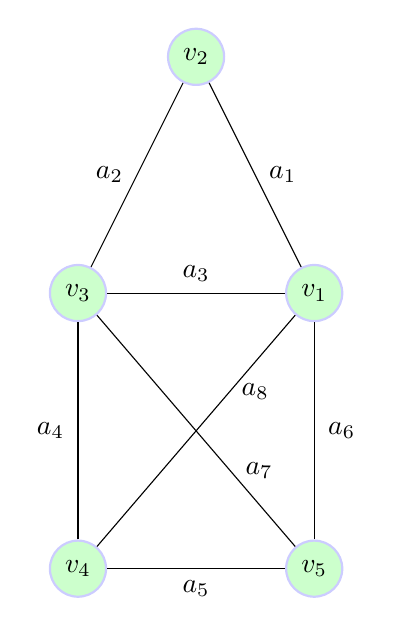
\begin{tikzpicture}{node distance=1.3cm,>=stealth',bend angle=45, auto}
  \tikzstyle{place}=[circle,thick,draw=blue!20,fill=green!20,minimum size=6mm]
  \tikzstyle{texto}=[]

  \begin{scope}

    \node [place] (c1) {$v_1$};

    \node [place] (c2) [above of=c1,xshift=-1.5cm,yshift=2cm] {$v_2$}
    edge [] node [xshift=.35cm] {$a_1$} (c1); 
    
    \node [place] (c3) [left of=c1, xshift=-2cm] {$v_3$}
    edge [] node [yshift=.25cm] {$a_3$} (c1) 
    edge [] node [xshift=-.35cm] {$a_2$} (c2);


    \node [place] (c4) [below of=c3,yshift=-2.5cm] {$v_4$}
    edge [] node [xshift=-.35cm] {$a_4$} (c3) 
    edge [] node [yshift=.5cm,xshift=.75cm] {$a_8$} (c1);

    \node [place] (c5) [below of=c1,yshift=-2.5cm] {$v_5$}
    edge [] node [yshift=-.25cm] {$a_5$} (c4)
    edge [] node [xshift=.35cm] {$a_6$} (c1)
    edge [] node [yshift=-.5cm,xshift=.8cm] {$a_7$} (c3);
\end{scope}  

\end{tikzpicture}
\end{minipage}%
\begin{minipage}{1cm}
\begin{center}
\[
 M =
 \begin{pmatrix}
  0 & 1 & 1 & 1 & 1 \\
  1 & 0 & 1 & 0 & 0 \\
  1 & 1 & 0 & 1 & 1 \\
  1 & 0 & 1 & 0 & 1 \\
  1 & 0 & 1 & 1 & 0 
 \end{pmatrix}
\]
\end{center}
\end{minipage}
\end{figure}%
\end{center}%
\begin{figure}[H]
\begin{center}
\caption{Grafo con su representación en matriz de adyacencia}%
\end{center}
\end{figure}

Con esta representación, es fácil ver si existe o no una arista entre dos nodos dados: buscar un valor en la matriz requiere un tiempo constante. Por otra parte, si deseamos examinar todos los nodos que estén conectados con algún nodo dado, tenemos que recorrer toda una fila completa de la matriz, en el caso de un grafo no dirigido, o bien tanto una fila completa como una columna completa en el caso de un grafo dirigido. Esto requiere un tiempo que está en $\Theta(V)$, el número de nodos que hay en el grafo, independientemente del número de aristas que entren o salgan de ese nodo particular. El espacio requerido para representar un grafo de esta manera es cuadrático con respecto al número de nodos.\\

La representación por matriz de adyacencia no es satisfactoria para la gran mayoría de grafos dispersos: necesitamos como mínimo para ello $V^2$ bits de almacenamiento y $V^2$ pasos sólo para la construcción de la matriz inicial representativa. En un grafo denso, donde el número de aristas (el número de 1 bit de la matriz) es proporcional a $V^2$, este coste puede ser aceptable, porque el tiempo proporcional a $V^2$ es el necesario para procesar las aristas sin importar la representación que se use en principio. En grafos dispersos, sin embargo, tan sólo la inicialización de la matriz podría ser el factor dominante en el tiempo de ejecución de un algoritmo. Por otra parte, tal vez ni siquiera habría suficiente espacio para la matriz de esa forma. Por ejemplo, podemos estar ante grafos con millones de vértices y decenas de millones de aristas, que sin embargo no tendrán que pagar el precio de reservar espacio en memoria para miles de millones de entradas con el valor 0 en la matriz de adyacencia.\\

Por otro lado, cuando es necesario procesar un grafo denso, las 0-entradas que representan ausencia de arista, incrementan nuestro espacio necesario sólo por un factor constante permitiéndonos determinar así, si cualquiera de las aristas está presente según la constante de tiempo. Si tenemos espacio disponible para almacenar una matriz de adyacencia y si $V^2$ es lo suficientemente pequeño como para ser representado en una cantidad insignificante de tiempo o para hacer uso de un algoritmo complejo que no requiera más de $V^2$ pasos para completarse, la representación mediante matriz de adyacencia puede ser el método de elección adecuado, sin importar lo denso que pueda ser el grafo.\\

\subsection{Matriz de incidencia}

La representación mediante matriz de incidencia de un grafo, es una matriz rectangular $v \times a$ de tantas filas como vértices $v = |V|$ tiene el grafo y tantas columnas como aristas $a = |A|$ hay. La entrada $(i,j)$ consiste en un 1 si el vértice $x_i$ es incidente con la arista $e_j$, siendo 0 en otro caso. Dado que cada arista incide en dos vértices (distintos), esta matriz verifica que cada columna contiene exactamente dos 1, siendo el resto de entradas 0. Toda matriz con esta propiedad es, de hecho, la matriz de incidencia de cierto grafo.

\begin{center}
\[
M = \bordermatrix{~ & a_1 & a_2 & a_3 & a_4 & a_5 & a_6 & a_7 & a_8 \cr
                  v_1 & 1 & 0 & 1 & 0 & 0 & 1 & 0 & 1 \cr
                  v_2 & 1 & 1 & 0 & 0 & 0 & 0 & 0 & 0 \cr
                  v_3 & 0 & 1 & 1 & 1 & 0 & 0 & 1 & 0 \cr
                  v_4 & 0 & 0 & 0 & 1 & 1 & 0 & 0 & 1 \cr
                  v_5 & 0 & 0 & 0 & 0 & 1 & 1 & 1 & 0 \cr}
\]
\end{center}
\begin{figure}[H]
\begin{center}
\caption{Matriz de incidencia del grafo de la Figura 2.9}
\end{center}
\end{figure}


\subsection{Listas de adyacencia}

La representación estándar preferida para representar grafos que no sean densos es la representación mediante listas de adyacencia, donde hacemos un seguimiento de todos los vértices conectados a cada vértice en una lista enlazada que está asociada con ese vértice. En la lista de adyacencia se asocia a cada nodo i una lista formada por sus vecinos, esto es, una lista formada por aquellos nodos j tales que existe una arista de i a j (en el caso de un grafo dirigido) o entre i y j (en el caso de un grafo no dirigido). Si el número de aristas del grafo es pequeño, esta representación utiliza menos espacio que la dada anteriormente. También puede que sea posible en este caso examinar todos los vecinos de un modo dado en menos de $V$ operaciones de análisis en el caso medio. Por otra parte, determinar si existe o no conexión directa entre dos nodos dados i y j nos obliga a recorrer la lista de vecinos del nodo i (y posiblemente también los del nodo j, en el caso de un grafo dirigido), lo cual es menos eficiente que buscar un valor booleano en una matriz.\\

\begin{center}%
\begin{figure}[H]%
\begin{minipage}[H]{1\columnwidth}%
\centering%
\begin{tikzpicture}{node distance=1.3cm,>=stealth',bend angle=45, auto}
    \matrix [matrix of nodes]
    {
      \node[minimum height=.85cm,draw,tokens=1,yshift=.135cm,label=left:\textcolor{black}{$0$}] (c1) {\ \ \ \ \ \ };&[1cm] \node[minimum height=.7375cm, minimum width=.75cm,draw,yshift=.135cm] (c2) {\ \ \ }; & \node[minimum height=.75cm, minimum width=.75cm,draw] (c3) {\ $6$\ };  &[1cm] \node[minimum height=.7375cm, minimum width=.75cm,draw,yshift=.135cm] (c4) {\ \ \ }; & \node[minimum height=.75cm, minimum width=.75cm,draw] (c5) {\ $5$\ }; & [1cm] \node[minimum height=.7375cm, minimum width=.75cm,draw,yshift=.135cm] (c6) {\ \ \ }; & \node[minimum height=.75cm, minimum width=.75cm,draw] (c7) {\ $1$\ }; & [1cm] \node[minimum height=.7375cm, minimum width=.75cm,draw,yshift=.135cm] (c8) {\ \ \ }; & \node[minimum height=.75cm, minimum width=.75cm,draw] (c9) {\ 2\ };\\
      \node[minimum height=.85cm,draw,tokens=1,yshift=.135cm,label=left:\textcolor{black}{$1$}] (d1) {\ \ \ \ \ \ };&[1cm] \node[minimum height=.7375cm, minimum width=.75cm,draw,yshift=.135cm] (d2) {\ \ \ }; & \node[minimum height=.75cm, minimum width=.75cm,draw] (d3) {\ $0$\ };   \\
      \node[minimum height=.85cm,draw,tokens=1,yshift=.135cm,label=left:\textcolor{black}{$2$}] (e1) {\ \ \ \ \ \ };&[1cm] \node[minimum height=.7375cm, minimum width=.75cm,draw,yshift=.135cm] (e2) {\ \ \ }; & \node[minimum height=.75cm, minimum width=.75cm,draw] (e3) {\ $0$\ };   \\
      \node[minimum height=.85cm,draw,tokens=1,yshift=.135cm,label=left:\textcolor{black}{$3$}] (f1) {\ \ \ \ \ \ }; &[1cm] \node[minimum height=.7375cm, minimum width=.75cm,draw,yshift=.135cm] (f2) {\ \ \ }; & \node[minimum height=.75cm, minimum width=.75cm,draw] (f3) {\ $5$ \ }; &[1cm] \node[minimum height=.7375cm, minimum width=.75cm,draw,yshift=.135cm] (f4) {\ \ \ }; & \node[minimum height=.75cm, minimum width=.75cm,draw] (f5) {\ $4$\ };  \\
      \node[minimum height=.85cm,draw,tokens=1,yshift=.135cm,label=left:\textcolor{black}{$4$}] (g1) {\ \ \ \ \ \ }; &[1cm] \node[minimum height=.7375cm, minimum width=.75cm,draw,yshift=.135cm] (g2) {\ \ \ }; & \node[minimum height=.75cm, minimum width=.75cm,draw] (g3) {\ $6$\ }; &[1cm] \node[minimum height=.7375cm, minimum width=.75cm,draw,yshift=.135cm] (g4) {\ \ \ }; & \node[minimum height=.75cm, minimum width=.75cm,draw] (g5) {\ $5$ \ }; &[1cm] \node[minimum height=.7375cm, minimum width=.75cm,draw,yshift=.135cm] (g6) {\ \ \ }; & \node[minimum height=.75cm, minimum width=.75cm,draw] (g7) {\ $3$ \ };  \\
      \node[minimum height=.85cm,draw,tokens=1,yshift=.135cm,label=left:\textcolor{black}{$5$}] (h1) {\ \ \ \ \ \ }; &[1cm] \node[minimum height=.7375cm, minimum width=.75cm,draw,yshift=.135cm] (h2) {\ \ \ }; & \node[minimum height=.75cm, minimum width=.75cm,draw] (h3) {\ $3$ \ }; &[1cm] \node[minimum height=.7375cm, minimum width=.75cm,draw,yshift=.135cm] (h4) {\ \ \ }; & \node[minimum height=.75cm, minimum width=.75cm,draw] (h5) {\ $0$ \ }; &[1cm] \node[minimum height=.7375cm, minimum width=.75cm,draw,yshift=.135cm] (h6) {\ \ \ }; & \node[minimum height=.75cm, minimum width=.75cm,draw] (h7) {\ $4$ \ };  \\
      \node[minimum height=.85cm,draw,tokens=1,yshift=.135cm,label=left:\textcolor{black}{$6$}] (i1) {\ \ \ \ \ \ }; &[1cm] \node[minimum height=.7375cm, minimum width=.75cm,draw,yshift=.135cm] (i2) {\ \ \ }; & \node[minimum height=.75cm, minimum width=.75cm,draw] (i3) {\ $0$\ }; &[1cm] \node[minimum height=.7375cm, minimum width=.75cm,draw,yshift=.135cm] (i4) {\ \ \ }; & \node[minimum height=.75cm, minimum width=.75cm,draw] (i5) {\ $4$\ };  \\
    };

    \draw (c1) to [post] (c2);
    \draw (c3) to [post] (c4);
    \draw (c5) to [post] (c6);
    \draw (c7) to [post] (c8);
    \draw (d1) to [post] (d2);
    \draw (e1) to [post] (e2);
    \draw (f1) to [post] (f2);
    \draw (f3) to [post] (f4);
    \draw (g1) to [post] (g2);
    \draw (g3) to [post] (g4);
    \draw (g5) to [post] (g6);
    \draw (h1) to [post] (h2);
    \draw (h3) to [post] (h4);
    \draw (h5) to [post] (h6);
    \draw (i1) to [post] (i2);
    \draw (i3) to [post] (i4);

\end{tikzpicture}
\caption{Listas de adyacencia}%
\end{minipage}%
\end{figure}%
\end{center}%

Para agregar una arista que conecte i e j, se añade j a la lista de adyacencia de i e i a la lista de adyacencia de j. De esta manera, podemos agregar nuevas aristas en tiempo constante, pero la cantidad total de espacio que utilizamos es proporcional al número de vértices más el número de aristas (en comparación con el número de vértices, que formarían un cuadrado en una matriz de adyacencia). Para los grafos no dirigidos, representaremos cada arista en dos lugares distintos: una arista que conecta con i e j se representa con nodos en ambas listas de adyacencia. \\

Con las listas de adyacencia, hay numerosas representaciones de un grafo dado incluso para una determinada numeración de vértices. No importa en qué orden aparezcan las aristas de las listas de adyacencia, ya que la estructura de la lista de adyacencia representará siempre al mismo grafo. Esta característica de las listas de adyacencia es importante para saber porque el orden en que las aristas aparecen en las listas afecta, a su vez, al orden en que las aristas son procesadas por los algoritmos. Es decir, la estructura de las listas de adyacencia determina como se comportará el grafo para el cálculo de un algoritmo sobre él. A pesar de que un algoritmo debe producir una solución correcta sin importar que las aristas estén ordenadas en las listas de adyacencia, se podría llegar a dicha solución por diferentes secuencias de procesamiento del algoritmo sobre diferentes ordenamientos. Si un algoritmo no necesita examinar todas las aristas del grafo para su cálculo, este efecto podría afectar al tiempo de desarrollo del algoritmo. Y, si hay más de una solución correcta, ordenamientos de entrada de aristas diferentes pueden llevar a resultados de salida diferentes.\\

\subsection{Principal ventaja de uso}

La principal ventaja de la representación de listas de adyacencia sobre la representación en matriz de adyacencia es que siempre se utiliza el espacio proporcional a $A + V$, frente a $V^2$ en la matriz de adyacencia. La principal desventaja es que la comprobación de la existencia de arista entre vértices puede llevar un tiempo proporcional a $V$, a diferencia del tiempo constante de la matriz de adyacencia. En estas características, en consecuencia, radica la diferencia entre el uso de listas de adyacencia enlazadas y vectores que representen el conjunto de vértices incidentes con los otros vértices del conjunto. \\

\section{Grados}
\subsection{Grado de un vértice}

\begin{fondo}
Llamaremos grado o valencia de un vértice al número de aristas que incidan en él.
\end{fondo}

Notaremos por $gr_G(v)$ al grado del vértice $v$ en el grafo $G$ y cuando no haya posibilidad de confusión notaremos, simplemente por $gr(v)$.\\

\underline{Algoritmo de comprobación Grado de un vértice}\\
\begin{Verbatim}[commandchars=\\\{\}]
\PY{c+cm}{/**}
\PY{c+cm}{ * Método observador}
\PY{c+cm}{ * @param vertice valor de tipo entero que se corresponde con el vértice}
\PY{c+cm}{ * o nodo del grafo.}
\PY{c+cm}{ * @param G matriz de adyacencia o de costes asociada al grafo.}
\PY{c+cm}{ * @return int: valor entero que se corresponde con la valencia del nodo.}
\PY{c+cm}{ * Número de valencia o grado de un vértice son las aristas }
\PY{c+cm}{ * incidentes en él que contenga.}
\PY{c+cm}{ */}

\PY{k+kd}{public} \PY{k+kt}{int} \PY{n+nf}{grado\PYZus{}vertice}\PY{o}{(}\PY{k+kt}{int} \PY{n}{vertice}\PY{o}{,} \PY{k+kt}{int} \PY{o}{[}\PY{o}{]}\PY{o}{[}\PY{o}{]} \PY{n}{G}\PY{o}{)}
\PY{o}{\PYZob{}}

    \PY{k+kt}{int} \PY{n}{grado}\PY{o}{=}\PY{l+m+mi}{0}\PY{o}{;}
    \PY{k+kt}{int} \PY{n}{tama\PYZus{}G} \PY{o}{=} \PY{n}{G}\PY{o}{.}\PY{n+na}{length}\PY{o}{;}

    \PY{k}{if}\PY{o}{(}\PY{n}{vertice} \PY{o}{<} \PY{l+m+mi}{0} \PY{o}{|}\PY{o}{|} \PY{n}{vertice} \PY{o}{>} \PY{n}{tama\PYZus{}G}\PY{o}{)}
	\PY{o}{\PYZob{}}
	    \PY{n}{System}\PY{o}{.}\PY{n+na}{out}\PY{o}{.}\PY{n+na}{println}\PY{o}{(}\PY{l+s}{"El vértice no esta en el grafo"}\PY{o}{)}\PY{o}{;}
	    \PY{k}{return} \PY{l+m+mi}{0}\PY{o}{;}
	\PY{o}{\PYZcb{}}

    \PY{k}{for}\PY{o}{(}\PY{k+kt}{int} \PY{n}{i}\PY{o}{=}\PY{l+m+mi}{0}\PY{o}{;} \PY{n}{i} \PY{o}{<} \PY{n}{tama\PYZus{}G}\PY{o}{;} \PY{o}{+}\PY{o}{+}\PY{n}{i}\PY{o}{)}
	\PY{o}{\PYZob{}}
	    \PY{k}{if}\PY{o}{(}\PY{n}{G}\PY{o}{[}\PY{n}{vertice}\PY{o}{]}\PY{o}{[}\PY{n}{i}\PY{o}{]} \PY{o}{!}\PY{o}{=} \PY{l+m+mi}{0}\PY{o}{)}
		\PY{n}{grado}\PY{o}{+}\PY{o}{+}\PY{o}{;}
	\PY{o}{\PYZcb{}}

    \PY{k}{return} \PY{n}{grado}\PY{o}{;}
\PY{o}{\PYZcb{}}
\end{Verbatim}


\subsection{Vértice aislado}

\begin{fondo}
Un vértice de grado cero se denomina aislado.
\end{fondo}

\subsection{Suma de los grados de un grafo}

\begin{fondo}
En cualquier grafo se verifica,
\begin{description}
\item[(a)] La suma de todos sus grados es igual al doble del número de sus aristas.
\item[(b)] El número de vértices de grado impar es par.
\end{description}
\end{fondo}

\figuratikz{1}{Grafo de ejemplo}
{
  \tikzstyle{place}=[circle,thick,draw=blue!20,fill=green!20,minimum size=6mm]
  \tikzstyle{texto}=[]

  \begin{scope}

    \node [place] (c1) {$v_4$};

    \node [place] (c2) [right of=c1,xshift=1.5cm,yshift=3cm] {$v_3$}
    edge [] (c1);

    \node [place] (c3) [right of=c1,xshift=1.5cm,yshift=-3cm] {$v_5$}
    edge [] (c1)
    edge [] (c2);

    \node [place] (c4) [right of=c2,xshift=3cm] {$v_2$}
    edge [] (c1)
    edge [] (c2)
    edge [] (c3);

    \node [place] (c5) [right of=c3,xshift=3cm] {$v_6$}
    edge [] (c1)
    edge [] (c2)
    edge [] (c3)
    edge [] (c4);

    \node [place] (c6) [above of=c5,yshift=2cm,xshift=2.75cm] {$v_1$}
    edge [] (c1)
    edge [] (c2)
    edge [] (c3)
    edge [] (c4)
    edge [] (c5);

\end{scope}  

}

Sea $G_1 = (V,A)$ siendo\\
\[ V = \{v_1,v_2,v_3,v_4,v_5,v_6\} \]
y\\
\[ A = \{v_1v_2,v_1v_3,v_1v_4,v_1v_5,v_1v_6,v_2v_3,v_2v_4,v_2v_5,v_2v_6,v_3v_4,v_3v_5,v_3v_6,v_4v_5,v_4v_6,v_5v_6\} \]
Entonces, $|A| = 15$ y $gr(v_i) = 5$, $i = 1,2,3,4,5,6$, luego
\[  \sum^{6}_{i=1}{gr(v_i) = 30 = 2 \cdot 15.5 = 2 |A|} \]
Por otra parte, todos los vértices son de grado impar, luego su número $(6)$ es par.\\

\subsection{Grado de entrada y de salida}

\begin{fondo}
Si $v$ es un vértice de un digrafo $D$, entonces su grado de entrada $gr_e(v)$ es el número de arcos en $D$ de la forma $uv$ y su grado de salida $gr_s(v)$ es el número de arcos en $D$ de la forma $vu$.
\end{fondo}

\section{Isomorfismo}

\subsection{Isomorfismo de grafos}

\begin{fondo}
Dos grafos $G_1 = (V_1,A_1)$ y $G_2 = (V_2,A_2)$ se dice que son isomorfos cuando existe una biyección entre los conjuntos de sus vértices que conserva la adyacencia. Si los grafos $G_1$ y $G_2$ son isomorfos, notaremos $G_1 \simeq G_2$.
\end{fondo}

Según la definición anterior,\\
\[ G_1 \simeq G_2 \iff \exists f\ : V_1 \rightarrow V_2\ : 
\left\{ 
  \begin{array}{l} 
    f\ \mbox{es biyectiva}  \\ 
    uv \in A_1 \iff f(u)(v) \in A_2; \forall u,v \in V_1
  \end{array} 
\right. \]

\figuratikz{1}{Tres grafos isomorfos entre sí}
{
  \tikzstyle{place}=[circle,thick,draw=blue!20,fill=green!20,minimum size=6mm]
  \tikzstyle{texto}=[]

  \begin{scope}

    \node [place] (c1) {$v_1$};

    \node [place] (c2) [right of=c1,xshift=.4cm] {$v_4$}
    edge [] (c1);

    \node [place] (c3) [right of=c2,yshift=1.2cm] {$v_2$}
    edge [] (c1)
    edge [] (c2);

    \node [place] (c4) [right of=c2,yshift=-1.2cm] {$v_3$}
    edge [] (c1)
    edge [] (c2)
    edge [] (c3);

    \node [place] (c5) [right of=c2,xshift=2cm] {$1$};

    \node [place] (c6) [right of=c5,xshift=1cm,yshift=1.5cm] {$2$}
    edge [] (c5);

    \node [place] (c7) [right of=c5,yshift=-1.5cm] {$4$}
    edge [] (c5)
    edge [] (c6);

    \node [place] (c8) [right of=c5,xshift=1.5cm,yshift=-.5cm] {$3$}
    edge [] (c5)
    edge [] (c6)
    edge [] (c7);

    \node [place] (c9) [right of=c8,xshift=1cm,yshift=.5cm] {$a$};
    
    \node [place] (c10) [right of=c9,xshift=1cm,yshift=1.5cm] {$b$}
    edge [] (c9);

    \node [place] (c11) [right of=c9,yshift=-1.5cm] {$d$}
    edge [] (c9);

    \node [place] (c12) [right of=c9,xshift=1.5cm,yshift=-.5cm] {$c$}
    edge [] (c9)
    edge [] (c10)
    edge [] (c11);

    \draw (c10) .. controls +(-150:2cm) and +(-25:-5cm) .. (c11);

\end{scope}  

}

\section{Subgrafos}

\subsection{Definición}

\begin{fondo}
Un subgrafo de un grafo $G = (V(G)),A(G))$ es un grafo $H = (V(H),A(H))$ tal que $V(H) \subseteq V(G)$ y $A(H) \subseteq A(G)$
\end{fondo}

\figuratikz{1}{Un grafo $G$ y tres de sus subgrafos}
{
  \tikzstyle{place}=[circle,thick,draw=blue!20,fill=green!20,minimum size=6mm]
  \tikzstyle{texto}=[]

  \begin{scope}

    \node [place] (c1) {$v_2$};

    \node [place] (c2) [right of=c1,xshift=1cm] {$v_1$}
    edge [] (c1);

    \node [place] (c3) [below of=c1,yshift=-1cm] {$v_3$}
    edge [] (c1)
    edge [] (c2);

    \node [place] (c4) [below of=c2,yshift=-1cm] {$v_4$}
    edge [] (c1)
    edge [] (c2)
    edge [] (c3);

    \node [texto] (t1) [below of=c3,yshift=.6cm,xshift=1.1cm] {$G$};

    \node [place] (c5) [right of=c2,xshift=.5cm] {$v_2$};

    \node [place] (c6) [right of=c5,xshift=1cm] {$v_1$}
    edge [] (c5);

    \node [place] (c7) [below of=c6,yshift=-1cm] {$v_4$}
    edge [] (c5)
    edge [] (c6);

    \node [texto] (t2) [below of=c7,yshift=.6cm,xshift=-1.2cm] {$H_1$};

    \node [place] (c8) [right of=c6,xshift=.5cm]{$v_2$};

    \node [place] (c9) [right of=c8,xshift=1cm] {$v_1$}
    edge [] (c8);

    \node [place] (c10) [below of=c8,yshift=-1cm] {$v_3$};

    \node [place] (c11) [below of=c9,yshift=-1cm] {$v_4$}
    edge [] (c8)
    edge [] (c9);

    \node [texto] (t3) [below of=c10,yshift=.6cm,xshift=1.1cm] {$H_2$};
    
    \node [place] (c12) [right of=c9,xshift=.5cm]{$v_2$};

    \node [texto] (c13) [right of=c12,xshift=1cm] {};

    \node [place] (c14) [below of=c12,yshift=-1cm] {$v_3$}
    edge [] (c12);

    \node [place] (c15) [below of=c13,yshift=-1cm] {$v_4$}
    edge [] (c14);

    \node [texto] (t4) [below of=c14,yshift=.6cm,xshift=1.1cm] {$H_3$};

\end{scope}  

}
\[G = \{v_1,v_2,v_3,v_4\},\{v_1v_2,v_1v_3,v_1v_4,v_2v_3,v_2v_4,v_3v_4\}\]
\[H_1 = \{v_1,v_2,v_4\},\{v_1v_2,v_1v_4,v_2v_4\}\]
\[H_2 = \{v_1,v_2,v_3,v_4\},\{v_1v_2,v_1v_4,v_2v_4\}\]
\[H_3 = \{v_2,v_3,v_4\},\{v_2v_3,v_3v_4\}\]
\subsection{Eliminación de aristas}

\begin{fondo}
Si $a$ es una arista del grafo $G$, entonces el subgrafo $G \setminus \{a\}$ es el grafo que se obtiene de $G$ eliminando la arista $a$.\\
En general, escribiremos $G \setminus \{a_1,a_2, \ldots, a_k\}$ para denominar al subgrafo que se obtiene de $G$ eliminando las aristas $a_1,a_2, \ldots, a_k$.
\end{fondo}

\subsection{Eliminación de vértices}

\begin{fondo}
Si $v$ es un vértice del grafo $G$, entonces el subgrafo $G \setminus \{v\}$ es el grafo que se obtiene de $G$ eliminando el vértice $v$.\\
En general, escribiremos $G \setminus \{v_1,v_2, \ldots, v_k\}$ para denominar al subgrafo que se obtiene de $G$ eliminando los vértices $v_1,v_2, \ldots, v_k$.
\end{fondo}

\section{Caminos y ciclos}

\subsection{Camino}

\begin{fondo}
Sea $G$ un grafo o un multigrafo. Un camino en $G$ es una sucesión donde se alternan vértices y aristas, comenzando y terminando con vértices y en el que cada arista es incidente con los dos vértices que la preceden y la siguen.
\end{fondo}

Un camino que une los vértices $v_1$ y $v_n$ sería:\\
\[v_1, v_1v_2, v_2, v_2v_3, \ldots, v_{n-1}, v_{n-1}v_n, v_n \]
Si se trata de un grafo (no un multigrafo) este camino también puede especificarse simplemente por la sucesión de sus vértices, $v_1, v_2, v_3, \ldots, v_{n-1}, v_n$ y lo representamos por:\\
\[ \gamma = \langle v_1, v_2, v_3, \ldots, v_{n-1}, v_n \rangle \]
A los vértices $v_1$ y $v_n$ se les denomina extremos del camino. Suele decirse también que el camino conecta $v_1$ con $v_n$ o que va de $v_1$ a $v_n$. La longitud del camino es el número $n-1$ de aristas que contiene.

Un camino es simple si en la sucesión de vértices no hay ninguno repetido.

\subsection{Ciclo}

\begin{fondo}
Sea $G$ un grafo o un multigrafo. Un ciclo en $G$ es un camino en el que sus extremos coinciden.\\

El ciclo será simple si no hay, además del primero y el último, ningún otro vértice repetido.
\end{fondo}

\figuratikz{1}{Caminos y Ciclos}
{
  \tikzstyle{place}=[circle,thick,draw=blue!20,fill=green!20,minimum size=6mm]
  \tikzstyle{texto}=[]

  \begin{scope}

    \node [place] (c1) {$v_5$};

    \node [place] (c2) [right of=c1,xshift=.5cm,yshift=3cm] {$v_4$};

    \node [place] (c3) [above of=c2,xshift=3cm] {$v_3$};

    \node [place] (c4) [right of=c1,xshift=3.5cm] {$v_6$};

    \node [place] (c5) [right of=c2,xshift=4.5cm] {$v_2$};

    \node [place] (c6) [right of=c4,xshift=3.5cm] {$v_1$};

    %\draw (c1) .. controls +(50:-2cm) and +(10:1cm) .. (c2);

    \draw (c1) .. controls +(-80:-2cm) and +(-100:2cm) .. (c2);
    \draw (c1) .. controls +(-10:1cm) and +(-10:-3cm) .. (c4);
    \draw (c2) .. controls +(10:1cm) and +(-10:-2cm) .. (c3);
    \draw (c2) .. controls +(-10:1cm) and +(-30:-1cm) .. (c4);
    \draw (c3) .. controls +(-60:2cm) and +(-70:-3cm) .. (c4);
    \draw (c3) .. controls +(-180:-1cm) and +(5:-1cm) .. (c5);
    \draw (c5) .. controls +(-150:2cm) and +(40:1cm) .. (c4);
    \draw (c5) .. controls +(-70:2cm) and +(150:1cm) .. (c6);

\end{scope}  

}

\quad $\gamma = \langle v_1,\ v_2,\ v_6,\ v_3,\ v_4,\ v_6,\ v_5 \rangle$ es un camino.\\

\quad $\gamma = \langle v_1,\ v_2,\ v_3,\ v_4 \rangle$ es un camino simple ya que no hay ningún vértice repetido.\\

\quad $\gamma = \langle v_1,\ v_2,\ v_6,\ v_5,\ v_4,\ v_6,\ v_2,\ v_1 \rangle$ es un ciclo.\\

\quad $\gamma = \langle v_2,\ v_3,\ v_4,\ v_5,\ v_6,\ v_2 \rangle$ es un ciclo simple ya que se repiten, únicamente, los \hspace*{.15in}{vértices primero y último.}\\


Un grafo acíclico no contiene ningún ciclo. Los árboles están conectados con los grafos no dirigidos acíclicos. Los árboles son los grafos más simples, y sus estructuras intrínsecamente recursivas, ya que la eliminación o corte de cualesquieras aristas deja como resultado dos pequeños árboles.

A los grafos dirigidos acíclicos se les llaman DAG. Estos surgen de forma natural en los problemas de horarios, donde una arista dirigida $(x,y)$ indica que la actividad de $x$ debe ocurrir antes que $y$. Una operación llamada \emph{ordenación topológica} ordena los vértices de un DAG según restricciones de precedencia en la ejecución o procesamiento de dichos elementos. La ordenación topológica es típicamente el primer paso para cualquier algoritmo sobre un DAG.

\begin{nota}
Se muestra una aproximación de comprobación de Aciclicidad para grafo dirigidos.\\
\end{nota}

\underline{Algoritmo de Comprobación de Aciclicidad}\\
\begin{Verbatim}[commandchars=\\\{\}]
\PY{c+cm}{/**}
\PY{c+cm}{ * Método observador. (para grafos dirigidos)}
\PY{c+cm}{ * Comprueba si un grafo dirigido es aciclico o no.}
\PY{c+cm}{ * @param G array multidimensional (matriz) que contiene la matriz}
\PY{c+cm}{ * de adyacencia del grafo G asociado.}
\PY{c+cm}{ * @return devuelve true o false (verdadero o falso) si se cumple}
\PY{c+cm}{ * que sea o no acíclico.}
\PY{c+cm}{ */}

\PY{k+kd}{public} \PY{k+kt}{boolean} \PY{n+nf}{AciclicoGD}\PY{o}{(}\PY{k+kt}{int} \PY{o}{[}\PY{o}{]}\PY{o}{[}\PY{o}{]} \PY{n}{G}\PY{o}{)}
\PY{o}{\PYZob{}}
	
    \PY{k+kt}{int} \PY{n}{tama\PYZus{}G} \PY{o}{=} \PY{n}{G}\PY{o}{.}\PY{n+na}{length}\PY{o}{;}
    \PY{k+kt}{int} \PY{n}{i}\PY{o}{;}
    \PY{k+kt}{boolean} \PY{n}{aciclico} \PY{o}{=} \PY{k+kc}{true}\PY{o}{;} 
    \PY{c+c1}{// El grafo es acíclico hasta que se demuestre lo contrario.}
    \PY{n}{visitados} \PY{o}{=} \PY{k}{new} \PY{k+kt}{boolean}\PY{o}{[}\PY{n}{tama\PYZus{}G}\PY{o}{]}\PY{o}{;}
    \PY{n}{ancestros} \PY{o}{=} \PY{k}{new} \PY{k+kt}{int}\PY{o}{[}\PY{n}{tama\PYZus{}G}\PY{o}{]}\PY{o}{;}
    \PY{c+c1}{// Para llevar la cuenta de los ancestros.}

    \PY{c+c1}{// Al comienzo no hay ningún vértice visitado.}
    \PY{n}{Arrays}\PY{o}{.}\PY{n+na}{fill}\PY{o}{(}\PY{n}{visitados}\PY{o}{,} \PY{k+kc}{false}\PY{o}{)}\PY{o}{;}

    \PY{c+cm}{/* Vamos iterando de componente en componente conexa}
\PY{c+cm}{       para sacar el árbol de expansión */}

    \PY{k}{for}\PY{o}{(}\PY{n}{i}\PY{o}{=}\PY{l+m+mi}{0}\PY{o}{;} \PY{n}{i} \PY{o}{<} \PY{n}{tama\PYZus{}G} \PY{o}{&}\PY{o}{&} \PY{n}{aciclico} \PY{o}{=}\PY{o}{=} \PY{k+kc}{true}\PY{o}{;} \PY{o}{+}\PY{o}{+}\PY{n}{i}\PY{o}{)}
	\PY{o}{\PYZob{}}
	    \PY{k}{if}\PY{o}{(}\PY{o}{!}\PY{n}{visitados}\PY{o}{[}\PY{n}{i}\PY{o}{]}\PY{o}{)}
		\PY{n}{aciclico} \PY{o}{=} \PY{n}{AciclicoGDRec}\PY{o}{(}\PY{n}{i}\PY{o}{,}\PY{n}{G}\PY{o}{,}\PY{l+m+mi}{0}\PY{o}{)}\PY{o}{;}
	\PY{o}{\PYZcb{}}
	
    \PY{k}{return} \PY{n}{aciclico}\PY{o}{;}
\PY{o}{\PYZcb{}}

\PY{c+cm}{/**}
\PY{c+cm}{ * Función privada de la clase que sirve para iterar sobre la estructura}
\PY{c+cm}{ * de aristas del grafo.}
\PY{c+cm}{ * @param vertice vértice inicial desde el que se realiza la búsqueda }
\PY{c+cm}{ * en el grafo.}
\PY{c+cm}{ * @param G array multidimensional (matriz) que contiene la matriz}
\PY{c+cm}{ * de adyacencia del grafo G asociado.}
\PY{c+cm}{ * @param num\PYZus{}ancestros número de vértices visitados anteriormente desde }
\PY{c+cm}{ * el vértice de partida.}
\PY{c+cm}{ * @return devuelve true o false (verdadero o falso) dependiendo de si }
\PY{c+cm}{ * encuentra un ciclo o no en la estructura.}
\PY{c+cm}{ */}

\PY{k+kd}{private} \PY{k+kt}{boolean} \PY{n+nf}{AciclicoGDRec}\PY{o}{(}\PY{k+kt}{int} \PY{n}{vertice}\PY{o}{,} \PY{k+kt}{int} \PY{o}{[}\PY{o}{]}\PY{o}{[}\PY{o}{]} \PY{n}{G}\PY{o}{,} \PY{k+kt}{int} \PY{n}{num\PYZus{}ancestros}\PY{o}{)} 
\PY{o}{\PYZob{}}
    \PY{k+kt}{int} \PY{n}{w}\PY{o}{=}\PY{l+m+mi}{0}\PY{o}{;}
    \PY{c+c1}{// Para movernos por los vértices adyacentes.}

    \PY{k+kt}{int} \PY{n}{i}\PY{o}{;}
    \PY{c+c1}{// Para movernos por los ancestros.}

    \PY{n}{visitados}\PY{o}{[}\PY{n}{vertice}\PY{o}{]} \PY{o}{=} \PY{k+kc}{true}\PY{o}{;}
    \PY{c+c1}{// Acabamos de visitar dicho vértice.}

    \PY{n}{ancestros}\PY{o}{[}\PY{n}{num\PYZus{}ancestros}\PY{o}{]} \PY{o}{=} \PY{n}{vertice}\PY{o}{;}
    \PY{c+c1}{// Guardamos el ancestro.}
	

    \PY{c+cm}{/* Ahora recorremos todos los vértices y miramos cuales son}
\PY{c+cm}{       adyacentes y de ellos los que no hemos visitado. Con estos}
\PY{c+cm}{       vértices seguimos la búsqueda en profundidad. */}

    \PY{k}{for}\PY{o}{(}\PY{n}{w}\PY{o}{=}\PY{l+m+mi}{0}\PY{o}{;} \PY{n}{w} \PY{o}{<} \PY{n}{G}\PY{o}{[}\PY{n}{vertice}\PY{o}{]}\PY{o}{[}\PY{n}{w}\PY{o}{]}\PY{o}{;} \PY{o}{+}\PY{o}{+}\PY{n}{w}\PY{o}{)}
	\PY{o}{\PYZob{}}
	    \PY{k}{if}\PY{o}{(}\PY{n}{G}\PY{o}{[}\PY{n}{vertice}\PY{o}{]}\PY{o}{[}\PY{n}{w}\PY{o}{]} \PY{o}{!}\PY{o}{=} \PY{l+m+mi}{0}\PY{o}{)}
		\PY{o}{\PYZob{}}
		    \PY{k}{if}\PY{o}{(}\PY{o}{!}\PY{n}{visitados}\PY{o}{[}\PY{n}{w}\PY{o}{]}\PY{o}{)}
			\PY{k}{return} \PY{o}{(}\PY{n}{AciclicoGDRec}\PY{o}{(}\PY{n}{w}\PY{o}{,}\PY{n}{G}\PY{o}{,}\PY{n}{num\PYZus{}ancestros}\PY{o}{+}\PY{o}{+}\PY{o}{)}\PY{o}{)}\PY{o}{;}
		    \PY{k}{else}
			\PY{o}{\PYZob{}}
			    \PY{c+c1}{// Si el vértice ya se ha visitado.}
			    \PY{k}{for}\PY{o}{(}\PY{n}{i}\PY{o}{=}\PY{l+m+mi}{0}\PY{o}{;} \PY{n}{i} \PY{o}{<}\PY{o}{=} \PY{n}{num\PYZus{}ancestros}\PY{o}{;} \PY{o}{+}\PY{o}{+}\PY{n}{i}\PY{o}{)}
				\PY{o}{\PYZob{}}
				    \PY{c+c1}{// Lo encontramos hay una arista.}
				    \PY{k}{if}\PY{o}{(}\PY{n}{ancestros}\PY{o}{[}\PY{n}{i}\PY{o}{]} \PY{o}{=}\PY{o}{=} \PY{n}{w}\PY{o}{)}
					\PY{k}{return} \PY{o}{(}\PY{k+kc}{false}\PY{o}{)}\PY{o}{;} \PY{c+c1}{//Hay un ciclo.}
					
				\PY{o}{\PYZcb{}}
			\PY{o}{\PYZcb{}}
		\PY{o}{\PYZcb{}}
	\PY{o}{\PYZcb{}}
	
    \PY{k}{return} \PY{o}{(}\PY{k+kc}{true}\PY{o}{)}\PY{o}{;} \PY{c+c1}{// Si llegamos aquí no se habrá encontrado ningún ciclo.}
\PY{o}{\PYZcb{}}
\end{Verbatim}


\section{Conexión en grafos}

Una de las propiedades más elementales de las que puede gozar cualquier grafo es que sea conexo.

\subsection{Vértices conectados}

\begin{fondo}
Dos vértices de un grafo se dice que están conectados cuando existe un camino entre ambos. Es decir,
\begin{center}$u$ y $v$ están conectados $\iff$ $\exists \mu = \langle u, v \rangle$ \end{center}
$\mu$ es un camino que une al vértice $u$ con el $v$.
\end{fondo}

\subsection{Grafos conexos}

\begin{fondo}
Un grafo se dice que es conexo si cada par de sus vértices están conectados. Es decir,
\begin{center} $G$ es conexo $\iff$ $\forall u, v$ : $\exists \mu = \langle u, v \rangle$ \end{center}
En caso contrario, diremos que $G$ es un grafo desconexo.
\end{fondo}

\figuratikz{1}{Ejemplos de grafos conexos}
{
  \tikzstyle{place}=[circle,thick,draw=blue!20,fill=green!20,minimum size=6mm]
  \tikzstyle{texto}=[]

  \begin{scope}

    \node [place] (c1) {$v_1$};

    \node [place] (c2) [right of=c1,xshift=1cm] {$v_2$}
    edge [] (c1);

    \node [place] (c3) [above of=c2,xshift=1cm] {$v_3$}
    edge [] (c2);

    \node [place] (c4) [right of=c3,yshift=-1cm,xshift=1cm] {$v_4$}
    edge [] (c3);

    \node [place] (c5) [below of=c3,xshift=.5cm] {$v_5$}
    edge [] (c4)
    edge [] (c3);

    \node [texto] (t1) [below of=c2,xshift=.7cm,yshift=.3cm] {Grafo conexo $G_1$};

    \node [place] (c6) [right of=c5,xshift=3cm] {$v_1$};

    \node [place] (c7) [right of=c6,xshift=1cm] {$v_2$}
    edge [] (c6);

    \node [place] (c8) [above of=c7,xshift=1cm] {$v_3$};

    \node [place] (c9) [right of=c8,yshift=-1cm,xshift=1cm] {$v_4$}
    edge [] (c8);

    \node [place] (c10) [below of=c8,xshift=.5cm] {$v_5$}
    edge [] (c9)
    edge [] (c8);

    \node [texto] (t2) [below of=c7,xshift=.7cm,yshift=.3cm] {Grafo desconexo $G_2$};


\end{scope}  

}

\subsection{Proposición}

\begin{fondo}
Dado un grafo, la relación ``estar conectado con'' definida en el conjunto de sus vértices es una relación de equivalencia.
\end{fondo}

\underline{Demostración}\\

Sea el grafo $G = (V,A)$ y definimos el conjunto $V$ de sus vértices la siguiente relación
\[ u {\cal{R}} v \iff u\ \mbox{está conectado con}\ v\]
Veamos que esta relación es de equivalencia.\\
\begin{description}
\item[(a)]\emph{Reflexividad}. Sea $u$ cualquiera de $V$. Entonces, el camino $\mu = \langle u, u \rangle$ conecta $u$ con \\ \hspace*{-.1in}{$u$, luego}
\[ \forall u \in V\ ; u {\cal{R}} u \]
\hspace*{-.1in}{es decir $\cal R$ es reflexiva.}
\item[(b)]\emph{Simetría}. Sea $u$ y $v$ dos elementos cualesquiera de $V$. Entonces,
\[ u {\cal{R}} v \iff \exists \mu = \langle u, v \rangle \Longrightarrow \exists \mu' = \langle u, v \rangle \iff v {\cal{R}} u \]
\hspace*{-.1in}{luego,}
\[ \forall u, v \in V ; u {\cal{R}} v \Longrightarrow v {\cal{R}} u \]
\hspace*{-.1in}{o sea, $\cal{R}$ es simétrica.}
\item[(c)]\emph{Transitividad}. Si $u,v$ y $w$ son tres vértices cualesquiera de $G$, entonces
\[
  \begin{array}{l}
    u {\cal{R}} v \iff \exists \mu_1 = \langle u, v \rangle \\
    v {\cal{R}} w \iff \exists \mu_2 = \langle v, w \rangle \\
  \end{array}
  \Biggl\} \Longrightarrow \exists \mu = \langle u, w \rangle \iff u {\cal{R}} w
\]
\hspace*{-.1in}{Bastaría, pues, con unir los caminos $\mu_1$ y $\mu_2$. Por lo tanto}
\[ \forall u, v, w ; u {\cal{R}} v \land v {\cal{R}} w \Longrightarrow u {\cal{R}} w \]
\hspace*{-.1in}{es decir, $\cal{R}$ es transitiva.}
\end{description}

\subsection{Componentes conexas de un grafo}

\begin{fondo}
Dado un grafo $G = (V,A)$, las clases de equivalencia en el conjunto de sus vértices, $V$, por la relación de equivalencia ``estar conectado con'' reciben el nombre de componentes conexas de $G$.
\end{fondo}

Obsérvese que de esta forma un grafo no conexo G puede ser ``partido'' por la relación anterior en subgrafos conexos que son las citadas componentes conexas de $G$.

\begin{ejem}
El conjunto de vértices del grafo $G_2$ de la figura 2.15 es
\[V = \{v_1, v_2, v_3, v_4, v_5 \} \]
y si consideramos en él la relación de equivalencia definida en la proposición anterior, las clases de equivalencia serán
\[ [v_1] = \{v_1, v_2\} = [v_2] \]
\[ [v_3] = \{v_3, v_4, v_5\} = [v_4] = [v_5] \]
Por lo tanto, el grafo $G_2$ tiene dos componentes conexas que son los subgrafos $H_1$ y $H_2$ cuyos conjuntos de vértices son $[v_1]$ y $[v_3]$, es decir,
\[ H_1 = (\{v_1, v_2\}, \{v_1v_2\}) \]
\[ H_2 = (\{v_3, v_4, v_5\}, \{v_3v_4, v_3v_5, v_4v_5\}) \]
\\
\end{ejem}

\begin{ejem}
Demostraremos que en un grafo conexo $G = (V,A)$ se verifica: $|V| - 1 \leq |A|$\\
\end{ejem}

\underline{Solución}

Utilizaremos la inducción sobre el número de vértices de $G$.

\emph{Paso básico.} Si $|V| = 1$, entonces $|A| = 0$, luego
\[ |V| - 1 = 1 - 1 = 0 = |A| \]

\emph{Paso inductivo.} Supongamos que la desigualdad es cierta para $|V| = p$ con $p > 1$ y veamos que también es cierta para $|V| = p + 1$.\\

En efecto, sea $u$ un vértice cualquier de $G$. Como el número de vértices, $p$, es mayor que 1, habrá otro vértice, $v$ en $G$ distinto de $u$ y, al ser $G$ conexo, deberá existir, al menos, un camino entre $u$ y $v$, luego $gr(v) \ge 1$.\\

\begin{itemize}
\item Si $gr(u) = 1$ y $a$ es la única arista que tiene a $u$ como extremo, entonces el grafo
\[(V \setminus \{u\}, A \setminus \{a\})\]
es conexo y tiene $p$ vértices. Por la hipótesis de inducción,\\
\[ |V \setminus \{u\}| -1 \leq |A \setminus \{a\}| \]
es decir,
\[ |V| - 2 \leq |A| -1 \]
de donde,
\[ |V| - 1 \leq |A| \]
\item Si $gr(u) > 1$, $\forall u \in V$, entonces por el teorema 2.9.4
\[ 2|V| \leq \mbox{Suma de los grados de los vértices de}\ G = 2|A| \]
o sea, $|V| \leq |A|$, de aquí que
\[ |V| - 1 < |A| \]
Por el \emph{primer principio de inducción matemática},
\[ |V| - 1 \leq |A| \]
\end{itemize}

\subsection{Puntos de corte}

\begin{fondo}
Dado un grafo conexo $G = (V,A)$, un vértice $u$ de $G$ se llama punto de corte cuando el subgrafo $G_u$ cuyos vértices son los de $V \setminus \{u\}$ y cuyas aristas son todas las de $A$ cuyos vértices están en $V \setminus \{u\}$ no es conexo.
\end{fondo}

Una consecuencia de esto es que uno de los conjuntos de corte produce exactamente dos componentes.\\

A veces es útil para indicar un conjunto límite fijado por la partición de los vértices que induce. Si $V$ denota al conjunto de vértices de $G$ y si $P$ es el subconjunto de vértices en una componente de $G$ inducida por el conjunto o punto de corte, entonces el límite del conjunto se puede especificar por $(P,\overline P)$ donde $\overline P = V - P$.\\

\begin{nota}
El algoritmo implementado verifica si existe algún punto de corte en el grafo. Hay otra versión que muestra dichos puntos de cortes del grafo.\\
\end{nota}

\underline{Algoritmo Comprobación Puntos de Corte}\\
\begin{Verbatim}[commandchars=\\\{\}]
\PY{c+cm}{/**}
\PY{c+cm}{ * Algoritmo de comprobación de vértices de corte - Método modificador.}
\PY{c+cm}{ * Muestra por la salida estándar los nodos de corte del grafo.}
\PY{c+cm}{ * @return boolean: representa un valor lógico que indica si se ha encontrado}
\PY{c+cm}{ * un punto de corte(true) o no(false) en el grafo.}
\PY{c+cm}{ * @exception Exception}
\PY{c+cm}{ */}

\PY{k+kd}{public} \PY{k+kt}{boolean} \PY{n+nf}{vertice\PYZus{}corte}\PY{o}{(}\PY{o}{)} \PY{k+kd}{throws} \PY{n}{Exception}
\PY{o}{\PYZob{}}
    \PY{n}{System}\PY{o}{.}\PY{n+na}{out}\PY{o}{.}\PY{n+na}{println}\PY{o}{(}\PY{l+s}{"Se procede a la búsqueda de vértice de corte"}\PY{o}{)}\PY{o}{;}
    \PY{n}{array\PYZus{}grados}\PY{o}{(}\PY{o}{)}\PY{o}{;}

    \PY{k+kt}{int} \PY{n}{tama\PYZus{}G} \PY{o}{=} \PY{k}{this}\PY{o}{.}\PY{n+na}{devolver\PYZus{}matriz}\PY{o}{(}\PY{o}{)}\PY{o}{.}\PY{n+na}{length}\PY{o}{;}
    \PY{k+kt}{int} \PY{n}{aux}\PY{o}{=}\PY{l+m+mi}{0}\PY{o}{;}
    \PY{k+kt}{boolean} \PY{n}{punto\PYZus{}corte}\PY{o}{=}\PY{k+kc}{true}\PY{o}{;}

    \PY{k}{for}\PY{o}{(}\PY{k+kt}{int} \PY{n}{i}\PY{o}{=}\PY{l+m+mi}{0}\PY{o}{;} \PY{n}{i} \PY{o}{<} \PY{n}{tama\PYZus{}G}\PY{o}{;} \PY{o}{+}\PY{o}{+}\PY{n}{i}\PY{o}{)}
	\PY{o}{\PYZob{}}
	    \PY{n}{aux} \PY{o}{=} \PY{n}{grados\PYZus{}interno}\PY{o}{.}\PY{n+na}{get}\PY{o}{(}\PY{n}{i}\PY{o}{)}\PY{o}{;}
	    \PY{k}{if}\PY{o}{(}\PY{k}{this}\PY{o}{.}\PY{n+na}{n\PYZus{}aristas}\PY{o}{(}\PY{o}{)} \PY{o}{-} \PY{n}{aux} \PY{o}{<} \PY{o}{(}\PY{k}{this}\PY{o}{.}\PY{n+na}{n\PYZus{}nodos}\PY{o}{(}\PY{o}{)} \PY{o}{-} \PY{l+m+mi}{1}\PY{o}{)}\PY{o}{)}
		\PY{n}{punto\PYZus{}corte} \PY{o}{=} \PY{k+kc}{false}\PY{o}{;}
	\PY{o}{\PYZcb{}}

    \PY{k}{return} \PY{n}{punto\PYZus{}corte}\PY{o}{;}
\PY{o}{\PYZcb{}}
\end{Verbatim}


\subsection{Puentes}

\begin{fondo}
Dado un grafo conexo $G = (V,A)$, a cualquier arista ``$a$'' de $G$ tal que el grafo $(V, A \setminus \{a\})$ no sea conexo, lo llamaremos puente.
\end{fondo}

\figuratikzno{1}{}{}
{
  \tikzstyle{place}=[circle,thick,draw=blue!20,fill=green!20,minimum size=6mm]
  \tikzstyle{texto}=[]

  \begin{scope}

    \node [place] (c1) {$v_6$};

    \node [place] (c2) [right of=c1,xshift=1cm,yshift=2.5cm] {$v_5$}
    edge [] (c1);

    \node [place] (c3) [right of=c1,xshift=1cm,yshift=-2.5cm] {$v_7$}
    edge [] (c1)
    edge [] (c2);

    \node [place] (c4) [right of=c2,xshift=2cm] {$v_4$}
    edge [] (c2);

    \node [place] (c5) [right of=c3,xshift=2cm] {$v_8$}
    edge [] (c4);

    \node [place] (c6) [right of=c1,xshift=6cm] {$v_3$}
    edge [] (c4)
    edge [] (c5);

    \node [place] (c7) [right of=c4,xshift=2.5cm] {$v_2$}
    edge [] (c6);

    \node [place] (c8) [right of=c5,xshift=2.5cm] {$v_9$}
    edge [] (c6);

    \node [place] (c9) [right of=c6,xshift=1.75cm] {$v_1$}
    edge [] (c7)
    edge [] (c8);

    \node [texto] (t1) [below of=c5,yshift=.2cm] {$G$};
\end{scope}  

}

Puntos de corte. Los vértices $v_3, v_4$ y $v_5$ ya que en la figura existen puntos que no pueden conectarse a través de ningún camino.\\

Puentes. El único puente que existe en el grafo propuesto es la arista $v_4v_5$ ya que en el grafo resultante existen vértices que no están conectados, es decir, no es conexo.\\
\begin{fondo}
Si $G = (V,A)$ es un grafo conexo y $a$ es una arista puente de $G$, entonces $(V,A \setminus \{a\})$ tiene exactamente dos componentes conexas.
\end{fondo}

\underline{Demostración}\\

Llamemos $v$ y $w$ a los vértices que son extremos de la arista $a$. Y dividamos los vértices de $G$ en dos clases:
\begin{enumerate}
\item El conjunto de vértices $V_1$, formado por aquellos para los que existe un camino que los conecta con $v$ \emph{sin usar} la arista $a$ (esto es, sin pasar por el vértice $w$). Entre estos está, por supuesto, el propio vértice $v$.
\item El conjunto de vértices $V_2$ de los vértices que \emph{necesariamente} han de usar la arista $a$ para conectarse a $v$. Entre ello está $w$.
\end{enumerate}

Que esto es una partición de los vértices de $G$ es obvio. Pero, además, la intersección de $V_1$ y $V_2$ es vacía: si un vértice $x \in V$ estuviera en $V_1$ y en $V_2$ a la vez, $a$ no sería arista puente, porque podríamos quitarla sin que se desconectara el grafo. Si ahora formamos el grafo $G = (V, A \setminus \{a\})$, sus dos componentes conexas son, precisamente, los vértices de $V_1$ (y sus aristas) y los vértices de $V_2$ (y sus aristas).\\

\underline{Algoritmo comprobación de Puentes}\\
\begin{Verbatim}[commandchars=\\\{\}]
\PY{c+cm}{/**}
\PY{c+cm}{ * Método modificador}
\PY{c+cm}{ * Método que halla las aristas de corte (puentes) de un grafo.}
\PY{c+cm}{ * @param G: matriz bidimensional de enteros que representa el grafo de}
\PY{c+cm}{ * trabajo actual.}
\PY{c+cm}{ */}

\PY{k+kd}{public} \PY{k+kt}{void} \PY{n+nf}{puentes}\PY{o}{(}\PY{k+kt}{int} \PY{o}{[}\PY{o}{]}\PY{o}{[}\PY{o}{]} \PY{n}{G}\PY{o}{)}
\PY{o}{\PYZob{}}
    \PY{k+kt}{int} \PY{n}{tama\PYZus{}G} \PY{o}{=} \PY{n}{G}\PY{o}{.}\PY{n+na}{length}\PY{o}{;}
    \PY{n}{hash\PYZus{}puentes} \PY{o}{=} \PY{k}{new} \PY{n}{HashMap}\PY{o}{<}\PY{n}{Integer}\PY{o}{,}\PY{n}{ArrayList}\PY{o}{<}\PY{n}{Integer}\PY{o}{>}\PY{o}{>}\PY{o}{(}\PY{o}{)}\PY{o}{;}
    \PY{n}{ArrayList}\PY{o}{<}\PY{n}{Integer}\PY{o}{>} \PY{n}{array\PYZus{}puentes}\PY{o}{;}
    \PY{n}{ArrayList}\PY{o}{<}\PY{n}{Arista}\PY{o}{>} \PY{n}{bridge} \PY{o}{=} \PY{k}{new} \PY{n}{ArrayList}\PY{o}{<}\PY{n}{Arista}\PY{o}{>}\PY{o}{(}\PY{o}{)}\PY{o}{;}
    \PY{n}{Arista} \PY{n}{I\PYZus{}J}\PY{o}{;}

    \PY{n}{grado\PYZus{}vector}\PY{o}{(}\PY{n}{G}\PY{o}{)}\PY{o}{;}
    \PY{k+kt}{boolean} \PY{n}{siguiente}\PY{o}{;}

    \PY{k}{for}\PY{o}{(}\PY{k+kt}{int} \PY{n}{i}\PY{o}{=}\PY{l+m+mi}{0}\PY{o}{;} \PY{n}{i} \PY{o}{<} \PY{n}{tama\PYZus{}G}\PY{o}{;} \PY{o}{+}\PY{o}{+}\PY{n}{i}\PY{o}{)}
	\PY{o}{\PYZob{}}
	    \PY{n}{array\PYZus{}puentes} \PY{o}{=} \PY{k}{new} \PY{n}{ArrayList}\PY{o}{<}\PY{n}{Integer}\PY{o}{>}\PY{o}{(}\PY{o}{)}\PY{o}{;}
		
	    \PY{k}{for}\PY{o}{(}\PY{k+kt}{int} \PY{n}{j}\PY{o}{=}\PY{l+m+mi}{0}\PY{o}{;} \PY{n}{j} \PY{o}{<} \PY{n}{tama\PYZus{}G}\PY{o}{;} \PY{o}{+}\PY{o}{+}\PY{n}{j}\PY{o}{)}
		\PY{o}{\PYZob{}}
		    \PY{k}{if}\PY{o}{(}\PY{n}{G}\PY{o}{[}\PY{n}{i}\PY{o}{]}\PY{o}{[}\PY{n}{j}\PY{o}{]} \PY{o}{!}\PY{o}{=} \PY{l+m+mi}{0}\PY{o}{)}
			\PY{n}{array\PYZus{}puentes}\PY{o}{.}\PY{n+na}{add}\PY{o}{(}\PY{n}{j}\PY{o}{)}\PY{o}{;}
		\PY{o}{\PYZcb{}}

	    \PY{n}{hash\PYZus{}puentes}\PY{o}{.}\PY{n+na}{put}\PY{o}{(}\PY{n}{i}\PY{o}{,}\PY{n}{array\PYZus{}puentes}\PY{o}{)}\PY{o}{;}

	\PY{o}{\PYZcb{}}
	
	
    \PY{k}{for}\PY{o}{(}\PY{k+kt}{int} \PY{n}{i}\PY{o}{=}\PY{l+m+mi}{0}\PY{o}{;} \PY{n}{i} \PY{o}{<} \PY{n}{tama\PYZus{}G}\PY{o}{;} \PY{o}{+}\PY{o}{+}\PY{n}{i}\PY{o}{)}
	\PY{k}{for}\PY{o}{(}\PY{k+kt}{int} \PY{n}{j}\PY{o}{=}\PY{l+m+mi}{0}\PY{o}{;} \PY{n}{j} \PY{o}{<} \PY{n}{hash\PYZus{}puentes}\PY{o}{.}\PY{n+na}{get}\PY{o}{(}\PY{n}{i}\PY{o}{)}\PY{o}{.}\PY{n+na}{size}\PY{o}{(}\PY{o}{)}\PY{o}{;} \PY{o}{+}\PY{o}{+}\PY{n}{j}\PY{o}{)}
	    \PY{o}{\PYZob{}}

		\PY{n}{I\PYZus{}J} \PY{o}{=} \PY{k}{new} \PY{n}{Arista}\PY{o}{(}\PY{o}{)}\PY{o}{;}
		\PY{n}{siguiente} \PY{o}{=} \PY{k+kc}{true}\PY{o}{;}

		\PY{k}{if}\PY{o}{(}\PY{n}{bridge}\PY{o}{.}\PY{n+na}{size}\PY{o}{(}\PY{o}{)} \PY{o}{!}\PY{o}{=} \PY{l+m+mi}{0}\PY{o}{)}
		    \PY{o}{\PYZob{}}
			\PY{k}{if}\PY{o}{(}\PY{n}{i} \PY{o}{=}\PY{o}{=} \PY{n}{bridge}\PY{o}{.}\PY{n+na}{get}\PY{o}{(}\PY{l+m+mi}{0}\PY{o}{)}\PY{o}{.}\PY{n+na}{v\PYZus{}destino}\PY{o}{(}\PY{o}{)} 
			   \PY{o}{&}\PY{o}{&} \PY{n}{hash\PYZus{}puentes}\PY{o}{.}\PY{n+na}{get}\PY{o}{(}\PY{n}{i}\PY{o}{)}\PY{o}{.}\PY{n+na}{get}\PY{o}{(}\PY{n}{j}\PY{o}{)} 
			   \PY{o}{=}\PY{o}{=} \PY{n}{bridge}\PY{o}{.}\PY{n+na}{get}\PY{o}{(}\PY{l+m+mi}{0}\PY{o}{)}\PY{o}{.}\PY{n+na}{v\PYZus{}origen}\PY{o}{(}\PY{o}{)}\PY{o}{)} 
			    \PY{o}{\PYZob{}}
				\PY{n}{siguiente} \PY{o}{=} \PY{k+kc}{false}\PY{o}{;}
				\PY{n}{bridge}\PY{o}{.}\PY{n+na}{remove}\PY{o}{(}\PY{l+m+mi}{0}\PY{o}{)}\PY{o}{;}
			    \PY{o}{\PYZcb{}}
				
		    \PY{o}{\PYZcb{}}

		\PY{k}{if}\PY{o}{(}\PY{n}{siguiente}\PY{o}{)}
		    \PY{k}{if}\PY{o}{(}\PY{n}{puentes\PYZus{}rec}\PY{o}{(}\PY{n}{i}\PY{o}{,}\PY{n}{hash\PYZus{}puentes}\PY{o}{.}\PY{n+na}{get}\PY{o}{(}\PY{n}{i}\PY{o}{)}\PY{o}{.}\PY{n+na}{get}\PY{o}{(}\PY{n}{j}\PY{o}{)}\PY{o}{,}\PY{n}{tama\PYZus{}G}\PY{o}{)}\PY{o}{)}
			\PY{o}{\PYZob{}}
			    \PY{n}{System}\PY{o}{.}\PY{n+na}{out}\PY{o}{.}\PY{n+na}{println}\PY{o}{(}\PY{l+s}{"Puente en: i:"}\PY{o}{+}\PY{n}{i}\PY{o}{+}\PY{l+s}{" j:"}
					       \PY{o}{+}\PY{n}{hash\PYZus{}puentes}\PY{o}{.}\PY{n+na}{get}\PY{o}{(}\PY{n}{i}\PY{o}{)}\PY{o}{.}\PY{n+na}{get}\PY{o}{(}\PY{n}{j}\PY{o}{)}\PY{o}{)}\PY{o}{;}
			    \PY{n}{I\PYZus{}J}\PY{o}{.}\PY{n+na}{v\PYZus{}origen}\PY{o}{(}\PY{n}{i}\PY{o}{)}\PY{o}{;}
			    \PY{n}{I\PYZus{}J}\PY{o}{.}\PY{n+na}{v\PYZus{}destino}\PY{o}{(}\PY{n}{hash\PYZus{}puentes}\PY{o}{.}\PY{n+na}{get}\PY{o}{(}\PY{n}{i}\PY{o}{)}\PY{o}{.}\PY{n+na}{get}\PY{o}{(}\PY{n}{j}\PY{o}{)}\PY{o}{)}\PY{o}{;}
			    \PY{n}{I\PYZus{}J}\PY{o}{.}\PY{n+na}{coste}\PY{o}{(}\PY{l+m+mi}{0}\PY{o}{)}\PY{o}{;}
			    \PY{n}{bridge}\PY{o}{.}\PY{n+na}{add}\PY{o}{(}\PY{n}{I\PYZus{}J}\PY{o}{)}\PY{o}{;}
			\PY{o}{\PYZcb{}}
	    \PY{o}{\PYZcb{}}	

\PY{o}{\PYZcb{}}

\PY{c+cm}{/**}
\PY{c+cm}{ * Método observador. (privado)}
\PY{c+cm}{ * Método recursivo que ayuda a la ejecución de la llamada principal de }
\PY{c+cm}{ * puentes. Comprueba si existe un puente para la arista de entrada como}
\PY{c+cm}{ * parámetro formal formada por sus vértices.}
\PY{c+cm}{ * @param u: valor entero que representa un extremo de la arista.}
\PY{c+cm}{ * @param v: valor entero que representa el otro extremo de la arista.}
\PY{c+cm}{ * @param tama\PYZus{}G: valor entero que representa el número de nodos del grafo.}
\PY{c+cm}{ * @return boolean: devolverá true o false dependiendo de si la arista}
\PY{c+cm}{ * es una arista de corte (puente) o no.}
\PY{c+cm}{ */}

\PY{k+kd}{private} \PY{k+kt}{boolean} \PY{n+nf}{puentes\PYZus{}rec}\PY{o}{(}\PY{k+kt}{int} \PY{n}{u}\PY{o}{,} \PY{k+kt}{int} \PY{n}{v}\PY{o}{,} \PY{k+kt}{int} \PY{n}{tama\PYZus{}G}\PY{o}{)}
\PY{o}{\PYZob{}}
    \PY{k+kt}{int} \PY{n}{pos\PYZus{}valencia}\PY{o}{=}\PY{l+m+mi}{0}\PY{o}{;}
    \PY{k+kt}{boolean} \PY{n}{camino}\PY{o}{=}\PY{k+kc}{false}\PY{o}{;}
    \PY{k+kt}{boolean} \PY{n}{fin}\PY{o}{=}\PY{k+kc}{false}\PY{o}{;}


    \PY{k+kt}{int} \PY{n}{i}\PY{o}{=}\PY{n}{u}\PY{o}{;}
    \PY{k+kt}{int} \PY{n}{ant\PYZus{}u}\PY{o}{=}\PY{n}{u}\PY{o}{;}
    \PY{k+kt}{int} \PY{n}{ant\PYZus{}v}\PY{o}{=}\PY{n}{v}\PY{o}{;} \PY{c+c1}{//Almacenamos los vértices origen.}

    \PY{n}{ArrayList}\PY{o}{<}\PY{n}{Integer}\PY{o}{>} \PY{n}{vertice\PYZus{}i} \PY{o}{=} \PY{k}{new} \PY{n}{ArrayList}\PY{o}{<}\PY{n}{Integer}\PY{o}{>}\PY{o}{(}\PY{o}{)}\PY{o}{;}
    \PY{n}{ArrayList}\PY{o}{<}\PY{n}{Integer}\PY{o}{>} \PY{n}{vertice\PYZus{}j} \PY{o}{=} \PY{k}{new} \PY{n}{ArrayList}\PY{o}{<}\PY{n}{Integer}\PY{o}{>}\PY{o}{(}\PY{o}{)}\PY{o}{;}

    \PY{k}{while}\PY{o}{(}\PY{o}{!}\PY{n}{fin}\PY{o}{)}
	\PY{o}{\PYZob{}}
	    \PY{c+cm}{/* Primero insertamos los nodos adyacentes de vertice\PYZus{}i (u)}
\PY{c+cm}{	       y luego hacemos lo mismo para los nodos adyacentes de}
\PY{c+cm}{	       vertice\PYZus{}j (v). Por ello cuando cambiemos los valores serán}
\PY{c+cm}{	       iteraciones pares (vertice\PYZus{}i) o impares (vertice\PYZus{}j).}
\PY{c+cm}{	    */}

	    \PY{k}{if}\PY{o}{(}\PY{n}{pos\PYZus{}valencia} \PY{o}{\PYZpc{}} \PY{l+m+mi}{2} \PY{o}{=}\PY{o}{=} \PY{l+m+mi}{0}\PY{o}{)}
		\PY{o}{\PYZob{}}

		    \PY{k}{if}\PY{o}{(}\PY{n}{vertice\PYZus{}i}\PY{o}{.}\PY{n+na}{size}\PY{o}{(}\PY{o}{)} \PY{o}{!}\PY{o}{=} \PY{l+m+mi}{0}\PY{o}{)}
			\PY{o}{\PYZob{}}
			    \PY{n}{ant\PYZus{}u} \PY{o}{=} \PY{n}{ant\PYZus{}v}\PY{o}{;}
			    \PY{n}{i} \PY{o}{=} \PY{n}{vertice\PYZus{}i}\PY{o}{.}\PY{n+na}{get}\PY{o}{(}\PY{l+m+mi}{0}\PY{o}{)}\PY{o}{;}
			    \PY{n}{vertice\PYZus{}i}\PY{o}{.}\PY{n+na}{remove}\PY{o}{(}\PY{l+m+mi}{0}\PY{o}{)}\PY{o}{;}


			    \PY{k}{for}\PY{o}{(}\PY{k+kt}{int} \PY{n}{j}\PY{o}{=}\PY{l+m+mi}{0}\PY{o}{;} \PY{n}{j} \PY{o}{<} \PY{n}{hash\PYZus{}puentes}\PY{o}{.}\PY{n+na}{get}\PY{o}{(}\PY{n}{i}\PY{o}{)}\PY{o}{.}\PY{n+na}{size}\PY{o}{(}\PY{o}{)}\PY{o}{;} \PY{o}{+}\PY{o}{+}\PY{n}{j}\PY{o}{)}
				\PY{o}{\PYZob{}}
				    \PY{c+cm}{/* En la primera estructura metemos }
\PY{c+cm}{				       los adyacentes del nodo u de la }
\PY{c+cm}{				       arista (u,v) */}

				    \PY{k}{if}\PY{o}{(}\PY{n}{hash\PYZus{}puentes}\PY{o}{.}\PY{n+na}{get}\PY{o}{(}\PY{n}{i}\PY{o}{)}\PY{o}{.}\PY{n+na}{get}\PY{o}{(}\PY{n}{j}\PY{o}{)} \PY{o}{!}\PY{o}{=} \PY{n}{ant\PYZus{}u}\PY{o}{)}
					\PY{n}{vertice\PYZus{}i}\PY{o}{.}\PY{n+na}{add}\PY{o}{(}\PY{n}{hash\PYZus{}puentes}\PY{o}{.}\PY{n+na}{get}\PY{o}{(}\PY{n}{i}\PY{o}{)}\PY{o}{.}\PY{n+na}{get}\PY{o}{(}\PY{n}{j}\PY{o}{)}\PY{o}{)}\PY{o}{;}
				\PY{o}{\PYZcb{}}
			\PY{o}{\PYZcb{}}
		    \PY{k}{else}\PY{o}{\PYZob{}}

			\PY{k}{if}\PY{o}{(}\PY{n}{hash\PYZus{}puentes}\PY{o}{.}\PY{n+na}{get}\PY{o}{(}\PY{n}{i}\PY{o}{)}\PY{o}{.}\PY{n+na}{size}\PY{o}{(}\PY{o}{)} \PY{o}{=}\PY{o}{=} \PY{l+m+mi}{1} 
			   \PY{o}{&}\PY{o}{&} \PY{n}{hash\PYZus{}puentes}\PY{o}{.}\PY{n+na}{get}\PY{o}{(}\PY{n}{i}\PY{o}{)}\PY{o}{.}\PY{n+na}{get}\PY{o}{(}\PY{l+m+mi}{0}\PY{o}{)} \PY{o}{=}\PY{o}{=} \PY{n}{v}\PY{o}{)}
			    \PY{o}{\PYZob{}}
				\PY{n}{fin} \PY{o}{=} \PY{k+kc}{true}\PY{o}{;}
				\PY{n}{camino} \PY{o}{=} \PY{k+kc}{true}\PY{o}{;}
			    \PY{o}{\PYZcb{}}

			\PY{k}{for}\PY{o}{(}\PY{k+kt}{int} \PY{n}{j}\PY{o}{=}\PY{l+m+mi}{0}\PY{o}{;} \PY{n}{j} \PY{o}{<} \PY{n}{hash\PYZus{}puentes}\PY{o}{.}\PY{n+na}{get}\PY{o}{(}\PY{n}{i}\PY{o}{)}\PY{o}{.}\PY{n+na}{size}\PY{o}{(}\PY{o}{)}\PY{o}{;} \PY{o}{+}\PY{o}{+}\PY{n}{j}\PY{o}{)}
			    \PY{o}{\PYZob{}}
				\PY{c+cm}{/* En la primera estructura metemos los }
\PY{c+cm}{				   adyacentes del nodo u de la arista (u,v) */}
	
				\PY{k}{if}\PY{o}{(}\PY{n}{hash\PYZus{}puentes}\PY{o}{.}\PY{n+na}{get}\PY{o}{(}\PY{n}{i}\PY{o}{)}\PY{o}{.}\PY{n+na}{get}\PY{o}{(}\PY{n}{j}\PY{o}{)} \PY{o}{!}\PY{o}{=} \PY{n}{v}\PY{o}{)}
				    \PY{n}{vertice\PYZus{}i}\PY{o}{.}\PY{n+na}{add}\PY{o}{(}\PY{n}{hash\PYZus{}puentes}\PY{o}{.}\PY{n+na}{get}\PY{o}{(}\PY{n}{i}\PY{o}{)}\PY{o}{.}\PY{n+na}{get}\PY{o}{(}\PY{n}{j}\PY{o}{)}\PY{o}{)}\PY{o}{;}
			    \PY{o}{\PYZcb{}}\PY{o}{\PYZcb{}}


		\PY{o}{\PYZcb{}}

	    \PY{k}{if}\PY{o}{(}\PY{n}{pos\PYZus{}valencia} \PY{o}{\PYZpc{}} \PY{l+m+mi}{2} \PY{o}{!}\PY{o}{=} \PY{l+m+mi}{0}\PY{o}{)}
		\PY{o}{\PYZob{}}
		    \PY{k}{if}\PY{o}{(}\PY{n}{vertice\PYZus{}j}\PY{o}{.}\PY{n+na}{size}\PY{o}{(}\PY{o}{)} \PY{o}{!}\PY{o}{=} \PY{l+m+mi}{0}\PY{o}{)}
			\PY{o}{\PYZob{}}
			    \PY{n}{ant\PYZus{}v} \PY{o}{=} \PY{n}{ant\PYZus{}u}\PY{o}{;}
			    \PY{n}{v} \PY{o}{=} \PY{n}{vertice\PYZus{}j}\PY{o}{.}\PY{n+na}{get}\PY{o}{(}\PY{l+m+mi}{0}\PY{o}{)}\PY{o}{;}
			    \PY{n}{vertice\PYZus{}j}\PY{o}{.}\PY{n+na}{remove}\PY{o}{(}\PY{l+m+mi}{0}\PY{o}{)}\PY{o}{;}
				
			    \PY{k}{for}\PY{o}{(}\PY{k+kt}{int} \PY{n}{j}\PY{o}{=}\PY{l+m+mi}{0}\PY{o}{;} \PY{n}{j} \PY{o}{<} \PY{n}{hash\PYZus{}puentes}\PY{o}{.}\PY{n+na}{get}\PY{o}{(}\PY{n}{v}\PY{o}{)}\PY{o}{.}\PY{n+na}{size}\PY{o}{(}\PY{o}{)}\PY{o}{;} \PY{o}{+}\PY{o}{+}\PY{n}{j}\PY{o}{)}
				\PY{o}{\PYZob{}}
				    \PY{c+cm}{/* En la segunda estructura metemos }
\PY{c+cm}{				       los adyacentes del nodo v de la }
\PY{c+cm}{				       arista (u,v) */}
		
				    \PY{k}{if}\PY{o}{(}\PY{n}{hash\PYZus{}puentes}\PY{o}{.}\PY{n+na}{get}\PY{o}{(}\PY{n}{v}\PY{o}{)}\PY{o}{.}\PY{n+na}{get}\PY{o}{(}\PY{n}{j}\PY{o}{)} \PY{o}{!}\PY{o}{=} \PY{n}{ant\PYZus{}v}\PY{o}{)}			    
					\PY{n}{vertice\PYZus{}j}\PY{o}{.}\PY{n+na}{add}\PY{o}{(}\PY{n}{hash\PYZus{}puentes}\PY{o}{.}\PY{n+na}{get}\PY{o}{(}\PY{n}{v}\PY{o}{)}\PY{o}{.}\PY{n+na}{get}\PY{o}{(}\PY{n}{j}\PY{o}{)}\PY{o}{)}\PY{o}{;}
					
				\PY{o}{\PYZcb{}}
				
			\PY{o}{\PYZcb{}}
		    \PY{k}{else}
			\PY{o}{\PYZob{}}


			    \PY{k}{if}\PY{o}{(}\PY{n}{hash\PYZus{}puentes}\PY{o}{.}\PY{n+na}{get}\PY{o}{(}\PY{n}{v}\PY{o}{)}\PY{o}{.}\PY{n+na}{size}\PY{o}{(}\PY{o}{)} \PY{o}{=}\PY{o}{=} \PY{l+m+mi}{1} 
			       \PY{o}{&}\PY{o}{&} \PY{n}{hash\PYZus{}puentes}\PY{o}{.}\PY{n+na}{get}\PY{o}{(}\PY{n}{v}\PY{o}{)}\PY{o}{.}\PY{n+na}{get}\PY{o}{(}\PY{l+m+mi}{0}\PY{o}{)} \PY{o}{=}\PY{o}{=} \PY{n}{u}\PY{o}{)}
				\PY{o}{\PYZob{}}
				    \PY{n}{fin} \PY{o}{=} \PY{k+kc}{true}\PY{o}{;}
				    \PY{n}{camino} \PY{o}{=} \PY{k+kc}{true}\PY{o}{;}
				\PY{o}{\PYZcb{}}

				    
			    \PY{k}{for}\PY{o}{(}\PY{k+kt}{int} \PY{n}{j}\PY{o}{=}\PY{l+m+mi}{0}\PY{o}{;} \PY{n}{j} \PY{o}{<} \PY{n}{hash\PYZus{}puentes}\PY{o}{.}\PY{n+na}{get}\PY{o}{(}\PY{n}{v}\PY{o}{)}\PY{o}{.}\PY{n+na}{size}\PY{o}{(}\PY{o}{)}\PY{o}{;} \PY{o}{+}\PY{o}{+}\PY{n}{j}\PY{o}{)}
				\PY{o}{\PYZob{}}
				    \PY{c+cm}{/* En la segunda estructura metemos }
\PY{c+cm}{				       los adyacentes del nodo}
\PY{c+cm}{				       v de la arista (u,v)*/}
					
				    \PY{k}{if}\PY{o}{(}\PY{n}{hash\PYZus{}puentes}\PY{o}{.}\PY{n+na}{get}\PY{o}{(}\PY{n}{v}\PY{o}{)}\PY{o}{.}\PY{n+na}{get}\PY{o}{(}\PY{n}{j}\PY{o}{)} \PY{o}{!}\PY{o}{=} \PY{n}{u}\PY{o}{)}			    
					\PY{n}{vertice\PYZus{}j}\PY{o}{.}\PY{n+na}{add}\PY{o}{(}\PY{n}{hash\PYZus{}puentes}\PY{o}{.}\PY{n+na}{get}\PY{o}{(}\PY{n}{v}\PY{o}{)}\PY{o}{.}\PY{n+na}{get}\PY{o}{(}\PY{n}{j}\PY{o}{)}\PY{o}{)}\PY{o}{;}
					
				\PY{o}{\PYZcb{}}
			\PY{o}{\PYZcb{}}
		\PY{o}{\PYZcb{}}
		
	    \PY{k}{for}\PY{o}{(}\PY{k+kt}{int} \PY{n}{j}\PY{o}{=}\PY{l+m+mi}{0}\PY{o}{;} \PY{n}{j} \PY{o}{<} \PY{n}{vertice\PYZus{}i}\PY{o}{.}\PY{n+na}{size}\PY{o}{(}\PY{o}{)} \PY{o}{&}\PY{o}{&} \PY{o}{!}\PY{n}{camino}\PY{o}{;} \PY{o}{+}\PY{o}{+}\PY{n}{j}\PY{o}{)}
		\PY{k}{for}\PY{o}{(}\PY{k+kt}{int} \PY{n}{k}\PY{o}{=}\PY{l+m+mi}{0}\PY{o}{;} \PY{n}{k} \PY{o}{<} \PY{n}{vertice\PYZus{}j}\PY{o}{.}\PY{n+na}{size}\PY{o}{(}\PY{o}{)} \PY{o}{&}\PY{o}{&} \PY{o}{!}\PY{n}{camino}\PY{o}{;} \PY{o}{+}\PY{o}{+}\PY{n}{k}\PY{o}{)}
		    \PY{o}{\PYZob{}}
		
			\PY{k}{if}\PY{o}{(}\PY{n}{vertice\PYZus{}i}\PY{o}{.}\PY{n+na}{get}\PY{o}{(}\PY{n}{j}\PY{o}{)} \PY{o}{=}\PY{o}{=} \PY{n}{vertice\PYZus{}j}\PY{o}{.}\PY{n+na}{get}\PY{o}{(}\PY{n}{k}\PY{o}{)}\PY{o}{)}
			    \PY{o}{\PYZob{}}
				\PY{c+cm}{/* Al llegar a este caso significa}
\PY{c+cm}{				   que se ha recorrido todo los nodos}
\PY{c+cm}{				   adyacentes posibles y no se ha hallado}
\PY{c+cm}{				   ningún camino auxiliar que conecte}
\PY{c+cm}{				   u y v. Por tanto (u,v) es una arista}
\PY{c+cm}{				   de corte.}
\PY{c+cm}{				*/}

				\PY{n}{camino} \PY{o}{=} \PY{k+kc}{false}\PY{o}{;}
				\PY{n}{fin} \PY{o}{=} \PY{k+kc}{true}\PY{o}{;}
			    \PY{o}{\PYZcb{}}
		    \PY{o}{\PYZcb{}}
	
	    \PY{n}{pos\PYZus{}valencia}\PY{o}{+}\PY{o}{+}\PY{o}{;}

	    \PY{k}{if}\PY{o}{(}\PY{n}{vertice\PYZus{}i}\PY{o}{.}\PY{n+na}{size}\PY{o}{(}\PY{o}{)} \PY{o}{=}\PY{o}{=} \PY{l+m+mi}{2}\PY{o}{)}
		\PY{k}{if}\PY{o}{(}\PY{n}{vertice\PYZus{}i}\PY{o}{.}\PY{n+na}{get}\PY{o}{(}\PY{l+m+mi}{0}\PY{o}{)} \PY{o}{=}\PY{o}{=} \PY{n}{vertice\PYZus{}i}\PY{o}{.}\PY{n+na}{get}\PY{o}{(}\PY{l+m+mi}{1}\PY{o}{)}\PY{o}{)}
		    \PY{o}{\PYZob{}}
			\PY{c+cm}{/* Al llegar a este caso significa}
\PY{c+cm}{			   que se ha encontrado un camino }
\PY{c+cm}{			   secundario para la arista (u,v),}
\PY{c+cm}{			   que conectaría los nodos u y v */}

			\PY{n}{fin} \PY{o}{=} \PY{k+kc}{true}\PY{o}{;}
			\PY{n}{camino} \PY{o}{=} \PY{k+kc}{true}\PY{o}{;}
		    \PY{o}{\PYZcb{}}

	    \PY{k}{if}\PY{o}{(}\PY{n}{vertice\PYZus{}j}\PY{o}{.}\PY{n+na}{size}\PY{o}{(}\PY{o}{)} \PY{o}{=}\PY{o}{=} \PY{l+m+mi}{2}\PY{o}{)}
		\PY{k}{if}\PY{o}{(}\PY{n}{vertice\PYZus{}j}\PY{o}{.}\PY{n+na}{get}\PY{o}{(}\PY{l+m+mi}{0}\PY{o}{)} \PY{o}{=}\PY{o}{=} \PY{n}{vertice\PYZus{}j}\PY{o}{.}\PY{n+na}{get}\PY{o}{(}\PY{l+m+mi}{1}\PY{o}{)}\PY{o}{)}
		    \PY{o}{\PYZob{}}
			\PY{c+cm}{/* Al llegar a este caso significa}
\PY{c+cm}{			   que se ha encontrado un camino }
\PY{c+cm}{			   secundario para la arista (u,v),}
\PY{c+cm}{			   que conectaría los nodos u y v */}

			\PY{n}{fin} \PY{o}{=} \PY{k+kc}{true}\PY{o}{;}
			\PY{n}{camino} \PY{o}{=} \PY{k+kc}{true}\PY{o}{;}
		    \PY{o}{\PYZcb{}}
	\PY{o}{\PYZcb{}}
    \PY{k}{return} \PY{n}{camino}\PY{o}{;}
		
\PY{o}{\PYZcb{}}
\end{Verbatim}



\section{Estructura de partición}

Un partición de un conjunto $C$ de elementos de un cierto tipo es un conjunto de subconjuntos disjuntos cuya unión es el conjunto total $C$.\\
Esta estructura se ha adaptado, en este caso, para representar particiones de elementos del tipo Arista cuyo representación interna es de la forma:
\[ Arista\ a\ =\ \langle x,y,z \rangle:
\left\{ 
\begin{array}{l}
x\ \mbox{el vértice origen}\\
y\ \mbox{el vértice destino}\\
z\ \mbox{el coste de la arista} 
\end{array}
\right. \]

Una relación de equivalencia sobre los elementos de un conjunto $C$ define una partición $C$ y, viceversa, cualquier partición de $C$ define una relación de equivalencia sobre sus elementos, de tal forma que cada miembro de la partición es una clase de equivalencia. Así pues, para cada subconjunto o clase podemos elegir cualquier elemento como representante canónico de todos sus miembros.\\

A continuación se da la especificación del TAD que representará la estructura de partición de nuestro sistema:\\

\underline{TAD Partición}\\
\begin{Verbatim}[commandchars=\\\{\}]
\PY{k+kd}{public} \PY{k+kd}{class} \PY{n+nc}{Particion}
\PY{o}{\PYZob{}}

    \PY{c+cm}{/**}
\PY{c+cm}{     * Atributos privados}
\PY{c+cm}{     */}

    \PY{c+cm}{/*}
\PY{c+cm}{      Array de enteros que contiene los padres}
\PY{c+cm}{      de las posiciones (nodos) del sistema.}
\PY{c+cm}{    */}

    \PY{k+kd}{private} \PY{k+kt}{int} \PY{o}{[}\PY{o}{]} \PY{n}{padre}\PY{o}{;}

    \PY{c+cm}{/*}
\PY{c+cm}{      Valor entero que cuyo contenido es}
\PY{c+cm}{      el número de nodos que posee el grafo.}
\PY{c+cm}{    */}

    \PY{k+kd}{private} \PY{k+kt}{int} \PY{n}{nEltos}\PY{o}{;}

    \PY{c+cm}{/**}
\PY{c+cm}{     * Constructor nulo.}
\PY{c+cm}{     */}

    \PY{k+kd}{public} \PY{n+nf}{Particion}\PY{o}{(}\PY{o}{)} \PY{o}{\PYZob{}}\PY{o}{\PYZcb{}}

    \PY{c+cm}{/**}
\PY{c+cm}{     * Constructor predeterminado.}
\PY{c+cm}{     * Se implementa un bosque de árboles (con control de altura). }
\PY{c+cm}{     * Compresión de caminos.}
\PY{c+cm}{     * @param n número de elementos de la partición que se crea}
\PY{c+cm}{     */}

    \PY{k+kd}{public} \PY{n+nf}{Particion}\PY{o}{(}\PY{k+kt}{int} \PY{n}{n}\PY{o}{)}
    \PY{o}{\PYZob{}}
	\PY{n}{padre} \PY{o}{=} \PY{k}{new} \PY{k+kt}{int}\PY{o}{[}\PY{n}{n}\PY{o}{]}\PY{o}{;}
	\PY{n}{nEltos} \PY{o}{=} \PY{n}{n}\PY{o}{;}

	\PY{n}{Arrays}\PY{o}{.}\PY{n+na}{fill}\PY{o}{(}\PY{n}{padre}\PY{o}{,}\PY{l+m+mi}{0}\PY{o}{,}\PY{n}{nEltos}\PY{o}{,}\PY{o}{-}\PY{l+m+mi}{1}\PY{o}{)}\PY{o}{;}
	\PY{c+c1}{//Creamos n árboles de altura 0 representada con -1}
    \PY{o}{\PYZcb{}}

    \PY{c+cm}{/**}
\PY{c+cm}{     * Método modificador.}
\PY{c+cm}{     * Une el subconjunto del elemento a y el del elemento b en uno }
\PY{c+cm}{     * de los subconjuntos arbitrariamente. La partición P queda }
\PY{c+cm}{     * con un miembro menos.}
\PY{c+cm}{     * @param a representante de la clase de partición (nodo).}
\PY{c+cm}{     * @param b representante de la clase de partición (nodo).}
\PY{c+cm}{     * @return void}
\PY{c+cm}{     */}
    
    \PY{k+kd}{public} \PY{k+kt}{void} \PY{n+nf}{Union}\PY{o}{(}\PY{k+kt}{int} \PY{n}{a}\PY{o}{,} \PY{k+kt}{int} \PY{n}{b}\PY{o}{)}
    \PY{o}{\PYZob{}}
	\PY{k}{if}\PY{o}{(}\PY{n}{padre}\PY{o}{[}\PY{n}{b}\PY{o}{]} \PY{o}{<} \PY{n}{padre}\PY{o}{[}\PY{n}{a}\PY{o}{]}\PY{o}{)}
	    \PY{n}{padre}\PY{o}{[}\PY{n}{a}\PY{o}{]} \PY{o}{=} \PY{n}{b}\PY{o}{;}
	\PY{k}{else}
	    \PY{o}{\PYZob{}}
	 	\PY{k}{if}\PY{o}{(}\PY{n}{padre}\PY{o}{[}\PY{n}{a}\PY{o}{]} \PY{o}{=}\PY{o}{=} \PY{n}{padre}\PY{o}{[}\PY{n}{b}\PY{o}{]}\PY{o}{)}
	 	    \PY{n}{padre}\PY{o}{[}\PY{n}{a}\PY{o}{]}\PY{o}{-}\PY{o}{-}\PY{o}{;}

	 	\PY{n}{padre}\PY{o}{[}\PY{n}{b}\PY{o}{]} \PY{o}{=} \PY{n}{a}\PY{o}{;}
	    \PY{o}{\PYZcb{}}
    \PY{o}{\PYZcb{}}

    \PY{c+cm}{/**}
\PY{c+cm}{     * Método observador.}
\PY{c+cm}{     * Devuelve el representante del subconjunto al que }
\PY{c+cm}{     * pertenece el elemento x.}
\PY{c+cm}{     * @param x elemento de la partición.}
\PY{c+cm}{     * @return devuelve el representante del subconjunto }
\PY{c+cm}{     * al que pertenece el elemento x.}
\PY{c+cm}{     */}

    \PY{k+kd}{public} \PY{k+kt}{int} \PY{n+nf}{Encontrar}\PY{o}{(}\PY{k+kt}{int} \PY{n}{x}\PY{o}{)}
    \PY{o}{\PYZob{}}
	\PY{k+kt}{int} \PY{n}{raiz}\PY{o}{,}\PY{n}{y}\PY{o}{;}

	\PY{n}{raiz} \PY{o}{=} \PY{n}{x}\PY{o}{;}

	\PY{k}{while}\PY{o}{(}\PY{n}{padre}\PY{o}{[}\PY{n}{raiz}\PY{o}{]} \PY{o}{>} \PY{o}{-}\PY{l+m+mi}{1}\PY{o}{)}
	    \PY{n}{raiz} \PY{o}{=} \PY{n}{padre}\PY{o}{[}\PY{n}{raiz}\PY{o}{]}\PY{o}{;}

	\PY{c+cm}{/* Los nodos del camino de x a raiz se hacen }
\PY{c+cm}{	   hijo de raiz. */}
	
	\PY{k}{while}\PY{o}{(}\PY{n}{padre}\PY{o}{[}\PY{n}{x}\PY{o}{]} \PY{o}{>}\PY{o}{=} \PY{n}{raiz}\PY{o}{)}
	    \PY{o}{\PYZob{}}
	 	\PY{n}{y} \PY{o}{=} \PY{n}{padre}\PY{o}{[}\PY{n}{x}\PY{o}{]}\PY{o}{;}
	 	\PY{n}{padre}\PY{o}{[}\PY{n}{x}\PY{o}{]} \PY{o}{=} \PY{n}{raiz}\PY{o}{;}
	 	\PY{n}{x} \PY{o}{=} \PY{n}{y}\PY{o}{;}
	    \PY{o}{\PYZcb{}}

	\PY{k}{return} \PY{n}{raiz}\PY{o}{;}
    \PY{o}{\PYZcb{}}

    
\PY{o}{\PYZcb{}}
\end{Verbatim}


La estructura de datos alternativa que se ha usado para la implementación de ciertas operaciones del TAD ha sido la de Bosque de Árboles. \\

La causa por la que operación \emph{Unión()} no se ejecuta en un tiempo constante es que para cada elemento se almacena el representante de su clase y esto obliga a modificar el representante de todos los elementos de uno de los conjuntos unidos. Podemos cambiar la estructura de datos para conseguir que la unión sea $O(1)$, pero a costa de empeorar el tiempo de ejecución de la operación \emph{Encontrar()}, ya que no existe una estructura de datos que permita ejecutar simultáneamente estas dos operaciones en un tiempo constante.\\

\vspace{-.3in}{\section{Disperso frente a denso}

Se define la densidad de un grafo como el promedio del grado de los vértices, o $2 A \setminus V$. Un grafo \emph{denso} es un grafo cuyo promedio de grado de vértices es proporcional a $V$; por otro lado un grafo disperso es un grafo cuyo complementario es denso. En otras palabras, consideramos que un grafo es denso si $A$ es proporcional a $V^2$ sino será disperso. Esta definición asintótica no es necesariamente significativa para un grafo en particular, pero la distinción es clara en general: Un grafo que cuenta con miles de vértices y miles de decenas de aristas es claramente disperso, y un grafo que tiene cientos de vértices y millones de aristas es claramente denso. Podríamos contemplar un grafo disperso con miles de millones de vértices, pero un grafo denso con miles de millones de vértices tendrá un numero abrumador de aristas. \\

Saber si un grafo es disperso o denso, es generalmente un factor clave en la selección de un algoritmo eficiente para procesar el grafo. Por ejemplo, para un problema en concreto, podríamos desarrollar un algoritmo que tomara alrededor de $V^2$ y otro que tomara alrededor de $A \lg A$ pasos. Estas fórmulas nos dicen que el segundo algoritmo sería mejor para grafos dispersos, mientras que el primero sería preferible para grafos densos. Por ejemplo, un grafo denso con millones de aristas podría tener sólo unos miles de vértices: en este caso $V^2$ y $A$ serían comparables en valor, y el algoritmo de $V^2$ pasos sería 20 veces más rápido que el algoritmo de $A \lg A$ pasos. Por otro lado, un grafo disperso con millones de aristas también tendría millones de vértices, por lo que el algoritmo de $A \lg A$ pasos podría ser millones de veces más rápido que el algoritmo de $V^2$ pasos. Podríamos hacer concesiones específicas sobre la base del análisis de estas fórmulas con más detalle, pero por lo general es suficiente en la práctica usar los términos disperso y denso de manera informal para ayudarnos a comprender las características fundamentales de rendimiento.\\}


\chapter{Algoritmos de grafos}
\label{chap:algoritmos}

\section{Caminos y ciclos de Euler}

En 1736, Leonhard Euler publicó un trabajo\footnote{Solutio problematis ad geometriam situs pertinentis (1741) (La solución a un problema relativo a la geometría de la posición).} en el cual resolvería el que ha venido a llamarse ``problema de los puentes de Königsberg''. La ciudad Königsberg (llamada Kaliningrado, durante la época soviética) estaba dividida por el río Pregel en cuatro zonas: las dos orillas (A y C), la isla llamada Kneiphof (B) y la parte comprendida entre las dos bifurcaciones del río. En aquel entonces había siete puentes comunicando las distintas zonas tal y como se observa en la figura. Parece ser que uno de los pasatiempos de los ciudadanos de Königsberg consistía en buscar un recorrido que travesase cada puente exactamente una vez. Se pensaba que tal paseo no era posible debido a los múltiples intentos fallidos pero que nadie había podido demostrar tal imposibilidad. Fue Euler quién demostró que la existencia de un tal recorrido requeriría, en general, que a lo sumo dos de las zonas estuvieran unidas con el resto mediante un número impar de puentes, cada una de ellas. Para probarlo, Euler reemplazó, en primer lugar, el mapa de la ciudad por un diagrama más simple, donde se incluye la información más relevante del problema, y, en segundo lugar, dio un razonamiento que sobrepasa el diagrama particular.\\

\vfill
\pagebreak

\figuratikz{1}{Problema de los puentes de Königsberg}
{
  \tikzstyle{place}=[circle,thick,draw=green!20,fill=blue!20,minimum size=5mm]
  \tikzstyle{texto}=[minimum size=5mm]

  \node [place] (c1) {$A$};

  \node [place] (c2) [right of=c1,xshift=2cm] {$B$}
  edge [bend right=20] node [above] {$2$} (c1)
  edge [bend left=20] node [below] {$3$} (c1);

  \node [place] (c3) [right of=c2,xshift=2cm] {$C$}
  edge [bend right=20] node [above] {$4$} (c2)
  edge [bend left=20] node [below] {$5$} (c2);

  \node [place] (c4) [above of=c2,yshift=4cm] {$D$}
  edge [bend right=30] node [above,yshift=.1cm,xshift=-.1cm] {$6$} (c1)
  edge [] node [left,xshift=-.1cm] {$1$} (c2)
  edge [bend left=30] node [above,yshift=.1cm,xshift=.1cm] {$7$} (c3);

}

Cabe mencionar la siguiente información:
\begin{itemize}
\item Euler no llegó a dibujar el diagrama de puntos y líneas que hoy conocemos como grafo (multigrafo) asociado al problema de los puentes de Königsberg.
\item Euler enunció, pero no demostró, que la condición necesaria dada por él también era suficiente. Su demostración se debe a Hierholzer (1873), quien al parecer desconocía el trabajo anterior de Euler. Hierholzer utiliza la expresión ``sistema de líneas entrelazadas'' para referirse a lo que hoy conocemos por grafo.
\end{itemize}

La principal aplicación fue la siguiente:
\begin{itemize}
\item El problema del cartero chino (Kwan Mei-Ko (1960)). Dicho problema se emplea para hallar la ruta óptima para un gps, etc. Además dicho problema tiene un algoritmo (algoritmo de Edmonds) de resolución en tiempo polinómico. En la base de dicho algoritmo se encuentra la observación de Goodman y Hedetniemi respecto a la equivalencia entre encontrar un recorrido de cartero de peso mínimo y la búsqueda de un conjunto de aristas de peso total mínimo cuya duplicación de lugar a un multigrafo Euleriano.
\end{itemize}

\subsection{Ciclo de Euler}

\begin{fondo}
Un ciclo de un grafo o multigrafo se dice de Euler si pasa todos los vértices recorriendo cada arista exactamente una vez.
\end{fondo}

\subsection{Grafo euleriano}

\begin{fondo}
Un grafo que admita un ciclo de Euler se denomina grafo Euleriano.
\end{fondo}

\subsection{Primer lema}

\begin{fondo}
Una condición necesaria para que un grafo o multigrafo sea Euleriano es que todos sus vértices sean de grado par.
\end{fondo}

\underline{Demostración}\\

En efecto, supongamos que $G$ es un grafo Euleriano, es decir, supongamos que existe un ciclo de Euler, $\gamma$, en $G$. Sea $v$ un vértice cualquiera de $G$. Veamos que tiene grado par.

\begin{itemize}
\item Si $v$ no es el primer vértice de $\gamma$, cada una de las veces que el ciclo pase por $v$ entrará y saldrá por dos aristas distintas de la vez anterior, luego contribuirá con 2 al grado de $v$.
\item Si $v$ es el primer vértice de $\gamma$, el ciclo $\gamma$ contribuye con 2 al grado de $v$ en cada una de las ``visitas'' que se realicen a $v$, salvo en la primera y en la última en la que añade 1 cada vez.
\end{itemize}

Por lo tanto, en cualquier caso, el grado de $v$ es par.\\

\textbf{Nota.}\\
\begin{center}%
\begin{figure}[H]%
\hspace*{-.2in}{\begin{minipage}[H]{.5\columnwidth}%
\centering%
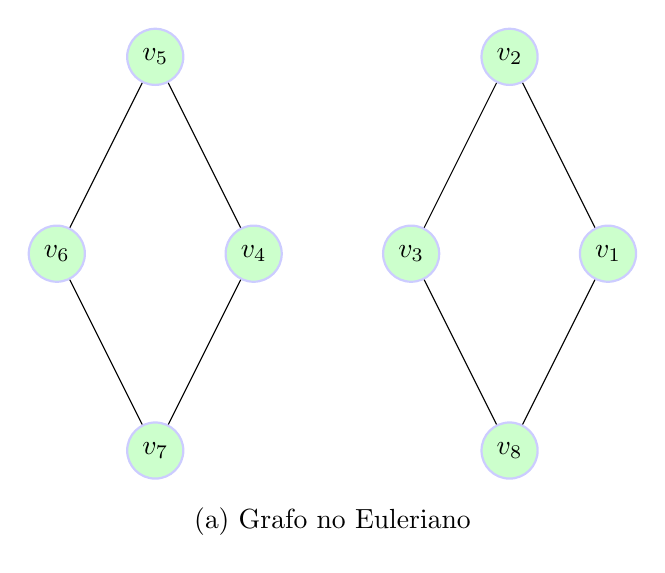
\begin{tikzpicture}{node distance=1.3cm,>=stealth',bend angle=45, auto}
  \tikzstyle{place}=[circle,thick,draw=blue!20,fill=green!20,minimum size=6mm]
  \tikzstyle{texto}=[]

  \begin{scope}

    \node [place] (c1) [xshift=-20cm]{$v_6$};

    \node [place] (c2) [right of=c1,xshift=.25cm,yshift=2.5cm] {$v_5$}
    edge [] (c1);

    \node [place] (c3) [right of=c1,xshift=.25cm,yshift=-2.5cm] {$v_7$}
    edge [] (c1);

    \node [place] (c4) [right of=c1,xshift=1.5cm] {$v_4$}
    edge [] (c2)
    edge [] (c3);

    \node [place] (c5) [right of=c4,xshift=1cm] {$v_3$};

    \node [place] (c6) [right of=c5,xshift=.25cm,yshift=2.5cm] {$v_2$}
    edge [] (c5);

    \node [place] (c7) [right of=c5,xshift=.25cm,yshift=-2.5cm] {$v_8$}
    edge [] (c5);

    \node [place] (c8) [right of=c5,xshift=1.5cm] {$v_1$}
    edge [] (c6)
    edge [] (c7);

    \node [texto] (p1) [below of=c7,yshift=.1cm,xshift=-2.25cm] {(a) Grafo no Euleriano};
  \end{scope}
\end{tikzpicture}
\end{minipage}}
\hspace*{.2in}{ \begin{minipage}{3cm}
\begin{center}
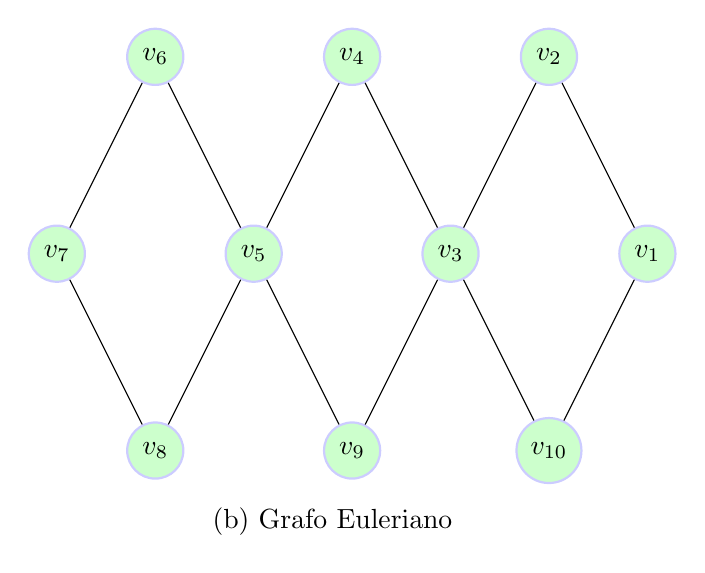
\begin{tikzpicture}{node distance=1.3cm,>=stealth',bend angle=45,auto}

  \tikzstyle{place}=[circle,thick,draw=blue!20,fill=green!20,minimum size=6mm]
  \tikzstyle{texto}=[]

  \begin{scope}


    \node [place] (t1) {$v_7$};

    \node [place] (t2) [right of=t1,xshift=.25cm,yshift=2.5cm] {$v_6$}
    edge [] (t1);

    \node [place] (t3) [right of=t1,xshift=.25cm,yshift=-2.5cm] {$v_8$}
    edge [] (t1);

    \node [place] (t4) [right of=t1,xshift=1.5cm] {$v_5$}
    edge [] (t2)
    edge [] (t3);

    \node [place] (t5) [right of=t4,xshift=1.5cm] {$v_3$};

    \node [place] (t6) [right of=t5,xshift=.25cm,yshift=2.5cm] {$v_2$}
    edge [] (t5);

    \node [place] (t7) [right of=t5,xshift=.25cm,yshift=-2.5cm] {$v_{10}$}
    edge [] (t5);

    \node [place] (t8) [right of=t5,xshift=1.5cm] {$v_1$}
    edge [] (t6)
    edge [] (t7);

    \node [place] (t9) [right of=t4,xshift=.25cm,yshift=2.5cm] {$v_4$}
    edge [] (t4)
    edge [] (t5);

    \node [place] (t10) [right of=t4,xshift=.25cm,yshift=-2.5cm] {$v_9$}
    edge [] (t4)
    edge [] (t5);

    \node [texto] (p1) [below of=t7,yshift=.1cm,xshift=-2.75cm] {(b) Grafo Euleriano};


\end{scope}  

\end{tikzpicture}

\end{center}
\end{minipage}}
\end{figure}
\end{center}

El grafo de la figura (a) nos muestra que la condición no es suficiente, es decir, existen grafos con todos los vértices de grado par y, sin embargo, no son eulerianos. Obsérvese que si \emph{conectamos} el grafo, entonces si es euleriano (apartado (b) de la figura). En efecto, el ciclo
\[ \gamma = \langle v_1, v_2, v_3, v_4, v_5, v_6, v_7, v_8, v_5, v_9, v_3, v_4, v_{10}, v_1 \rangle \]
es de Euler.\\

\begin{nota}
En el Primer Lema hemos visto que\\
\begin{center} Si $G$ es un Grafo Euleriano, entonces todos sus vértices son de grado par. \end{center}
de donde negando ambos miembros, y teniendo en cuenta la equivalencia lógica entre una proposición condicional y su contrarrecíproca, tendremos
\begin{center} Si existe algún vértice de grado impar, entonces $G$ no es Euleriano. \end{center}
es decir, si en un Grafo $G$ existe, al menos, un vértice de grado impar, entonces no es Euleriano.\\
\end{nota}

\subsection{Camino de Euler}

\begin{fondo}
Se dice que un camino de un grafo o multigrafo es de Euler si pasa por todos los vértices del mismo, recorriendo cada arista del mismo exactamente una vez.
\end{fondo}

Obsérvese que un \emph{camino de Euler} en un grafo $G$ puede entenderse también como una forma de dibujar el grafo sin levantar el lápiz del papel y sin pintar dos veces la misma arista.\\

\begin{nota}
El algoritmo implementado para el Camino de Euler comprueba la existencia de dicho camino o no. Hay otra versión que muestra en la salida estándar del sistema uno de los caminos posibles hallados.\\
\end{nota}

\underline{Camino de Euler}\\
\begin{Verbatim}[commandchars=\\\{\}]
\PY{c+cm}{/**}
\PY{c+cm}{ * Método observador (Euler dirigido)}
\PY{c+cm}{ * Método que llama al procedimiento general para la obtención del camino}
\PY{c+cm}{ * euleriano (si existe) del grafo euleriano (si lo es).}
\PY{c+cm}{ * @param G: matriz bidimensional de enteros cuyo contenido es el grafo}
\PY{c+cm}{ * de trabajo actual.}
\PY{c+cm}{ * @param v: valor entero que representa el nodo origen para el camino}
\PY{c+cm}{ * euleriano.}
\PY{c+cm}{ * @param w: valor entero que representa el nodo anterior procesado }
\PY{c+cm}{ * (en la primera llamada será el mismo nodo que v).}
\PY{c+cm}{ * @return boolean: devuelve true o fale si hay encontrado o no un }
\PY{c+cm}{ * camino euleriano para el grafo.}
\PY{c+cm}{ */}
    
\PY{k+kd}{public} \PY{k+kt}{boolean} \PY{n+nf}{camino\PYZus{}eulerGD}\PY{o}{(}\PY{k+kt}{int} \PY{o}{[}\PY{o}{]}\PY{o}{[}\PY{o}{]} \PY{n}{G}\PY{o}{,} \PY{k+kt}{int} \PY{n}{v}\PY{o}{,} \PY{k+kt}{int} \PY{n}{w}\PY{o}{)}
\PY{o}{\PYZob{}}
    \PY{n}{vert\PYZus{}orig\PYZus{}euler} \PY{o}{=} \PY{n}{w}\PY{o}{;}
    \PY{n}{algo\PYZus{}EulerGD}\PY{o}{(}\PY{n}{G}\PY{o}{,}\PY{n}{v}\PY{o}{,}\PY{n}{w}\PY{o}{)}\PY{o}{;}
	

    \PY{k}{return} \PY{n}{encontrado\PYZus{}euler}\PY{o}{;}
\PY{o}{\PYZcb{}}


\PY{c+cm}{/**}
\PY{c+cm}{ * Método modificador (Algoritmo Euler para grafos dirigidos)}
\PY{c+cm}{ * Un camino euleriano: un camino partiendo de un nodo origen que}
\PY{c+cm}{ * pase por todos los vértices (se pueden repetir) empleando todas}
\PY{c+cm}{ * las aristas posibles y regresando al nodo origen (ciclo).}
\PY{c+cm}{ * @param G: matriz bidimensional de enteros cuyo contenido es el grafo}
\PY{c+cm}{ * de trabajo actual.}
\PY{c+cm}{ * @param v: valor entero que representa el nodo origen para el camino}
\PY{c+cm}{ * euleriano.}
\PY{c+cm}{ * @param w: valor entero que representa el nodo anterior procesado }
\PY{c+cm}{ * (en la primera llamada será el mismo nodo que v).}
\PY{c+cm}{ */}

\PY{k+kd}{private} \PY{k+kt}{void} \PY{n+nf}{algo\PYZus{}EulerGD}\PY{o}{(}\PY{k+kt}{int} \PY{o}{[}\PY{o}{]}\PY{o}{[}\PY{o}{]} \PY{n}{G}\PY{o}{,} \PY{k+kt}{int} \PY{n}{v}\PY{o}{,} \PY{k+kt}{int} \PY{n}{w}\PY{o}{)}
\PY{o}{\PYZob{}}
    \PY{n}{grado\PYZus{}vector}\PY{o}{(}\PY{n}{G}\PY{o}{)}\PY{o}{;}
    \PY{k+kt}{int} \PY{n}{tama\PYZus{}G} \PY{o}{=} \PY{n}{G}\PY{o}{.}\PY{n+na}{length}\PY{o}{;}
    \PY{k+kt}{int} \PY{n}{t} \PY{o}{=} \PY{n}{grado\PYZus{}euler}\PY{o}{[}\PY{n}{v}\PY{o}{]} \PY{o}{+} \PY{n}{grado\PYZus{}euler}\PY{o}{[}\PY{n}{w}\PY{o}{]}\PY{o}{;}
    \PY{n}{dirigido\PYZus{}euler} \PY{o}{=} \PY{k+kc}{true}\PY{o}{;}

    \PY{n}{v\PYZus{}euler} \PY{o}{=} \PY{n}{v}\PY{o}{;}
    \PY{n}{pila\PYZus{}euler} \PY{o}{=} \PY{k}{new} \PY{n}{Stack}\PY{o}{<}\PY{n}{Integer}\PY{o}{>}\PY{o}{(}\PY{o}{)}\PY{o}{;}
    \PY{n}{hash\PYZus{}euler} \PY{o}{=} \PY{k}{new} \PY{n}{HashMap}\PY{o}{<}\PY{n}{Integer}\PY{o}{,}\PY{n}{ArrayList}\PY{o}{<}\PY{n}{Integer}\PY{o}{>}\PY{o}{>}\PY{o}{(}\PY{o}{)}\PY{o}{;}
    \PY{n}{ArrayList}\PY{o}{<}\PY{n}{Integer}\PY{o}{>} \PY{n}{adyacencias}\PY{o}{;}

    \PY{k}{for}\PY{o}{(}\PY{k+kt}{int} \PY{n}{i}\PY{o}{=}\PY{l+m+mi}{0}\PY{o}{;} \PY{n}{i} \PY{o}{<} \PY{n}{tama\PYZus{}G}\PY{o}{;} \PY{o}{+}\PY{o}{+}\PY{n}{i}\PY{o}{)}
	\PY{o}{\PYZob{}}
	    \PY{n}{adyacencias} \PY{o}{=} \PY{k}{new} \PY{n}{ArrayList}\PY{o}{<}\PY{n}{Integer}\PY{o}{>}\PY{o}{(}\PY{o}{)}\PY{o}{;}

	    \PY{k}{for}\PY{o}{(}\PY{k+kt}{int} \PY{n}{j}\PY{o}{=}\PY{l+m+mi}{0}\PY{o}{;} \PY{n}{j} \PY{o}{<} \PY{n}{tama\PYZus{}G}\PY{o}{;} \PY{o}{+}\PY{o}{+}\PY{n}{j}\PY{o}{)}
		\PY{o}{\PYZob{}}
		    \PY{k}{if}\PY{o}{(}\PY{n}{G}\PY{o}{[}\PY{n}{i}\PY{o}{]}\PY{o}{[}\PY{n}{j}\PY{o}{]} \PY{o}{!}\PY{o}{=} \PY{l+m+mi}{0}\PY{o}{)}
			\PY{o}{\PYZob{}}

			    \PY{n}{adyacencias}\PY{o}{.}\PY{n+na}{add}\PY{o}{(}\PY{n}{j}\PY{o}{)}\PY{o}{;}
			\PY{o}{\PYZcb{}}
		\PY{o}{\PYZcb{}}

	    \PY{n}{hash\PYZus{}euler}\PY{o}{.}\PY{n+na}{put}\PY{o}{(}\PY{n}{i}\PY{o}{,}\PY{n}{adyacencias}\PY{o}{)}\PY{o}{;}
	\PY{o}{\PYZcb{}}

    \PY{n}{encontrado\PYZus{}euler} \PY{o}{=} \PY{n}{entrada\PYZus{}salida\PYZus{}euler}\PY{o}{(}\PY{n}{G}\PY{o}{.}\PY{n+na}{length}\PY{o}{)}\PY{o}{;}

\PY{o}{\PYZcb{}}
\end{Verbatim}


\subsection{Segundo lema}

\begin{fondo}
Una condición necesaria para que un grafo o multigrafo admita un camino de Euler es que el número de vértices de grado impar sea 2 o ninguno.
\end{fondo}

\underline{Demostración}\\

Sea $G = (V,A)$ un grafo con un camino de Euler $\gamma = \langle u, u_1, u_2, \ldots, u_p, v \rangle$. \\
Tomamos un punto $w$ que no pertenezca a $V$ y sea $G' = (V',A')$ un grafo tal que
\[V' = V \cup \{w\} \]
\[ A' = A \cup \{uw, vw\} \]
es decir, el grafo obtenido añadiendo el nuevo punto como vértice al grafo original y las dos aristas adyacentes al mismo y a los extremos $u$ y $v$.\\
El ciclo
\[ \langle w, u, u_1, \ldots, u_p, v, w \rangle \]
es de Euler en $G'$, de aquí que $G'$ sea un grafo euleriano y aplicando el \emph{primer lema}, tengamos que todos sus vértices son de grado par.\\
Pues bien, si $x$ es cualquier vértice de $G$ distinto de $u$ y de $v$, entonces
\[ gr_G(x) = gr_{G'}(x) \]
luego el grado de $x$ en el grafo $G$ es par. Por otra parte,
\[ \begin{array}{l c}
  & gr_G(u) = gr_{G'}(u) - 1 \Longrightarrow gr_G(u)\ \mbox{es impar} \\
  \mbox{y} &\\
  & gr_G(v) = gr_{G'}(v) - 1 \Longrightarrow gr_G(v)\ \mbox{es impar}
\end{array} \]

luego los únicos dos vértices de grado impar son $u$ y $v$.\\

\begin{nota}
En el segundo lema, hemos visto que
\begin{quote}
\emph{``Si $G$ es un grafo con un camino de Euler, entonces el número de vértices de grado impar es 2 o ninguno''}
\end{quote}
Si ahora negamos ambos miembros, y tenemos en cuenta la equivalencia lógica entre una proposición condicional y su contrarrecíproca, tendremos
\begin{quote}
\emph{``Si el número de vértices de grado impar es distinto de 2, entonces $G$ no tiene ningún camino de Euler''}
\end{quote}
\end{nota}

\subsection{Tercer lema}

\begin{fondo}
Si $G$ es un grafo en el que todos sus vértices tienen grado par, entonces para cada par de vértices adyacentes de $G$, puede encontrarse un ciclo que contiene a la arista que forman ambos.
\end{fondo}

\underline{Demostración}\\
\\
Sean $u$ y $v$ dos vértices adyacentes de $G$ y sea $\gamma$ un camino que comienza en $u$ y continúa por la arista $uv$.\\
\\
Cada vez que $\gamma$ llega a un vértice $w$ distinto de $u$, continuamos el camino por una arista que no esté en $\gamma$, si $w$ es igual a $u$ damos por terminado el proceso. Dado que los grados de los vértices son pares por hipótesis, cada vez que el camino $\gamma$ pasa por un vértice utiliza dos aristas con un extremo en el mismo. Como el número de aristas y el de vértices es finito, el camino $\gamma$ acaba por volver a $u$ y $\gamma$ es, según la construcción hecha, un ciclo. \\


\section{Caminos y ciclos de Hamilton}

Se dice que el matemático irlandés William Hamilton (1805-1865) en el año 1857 inventó un juego que consistía en buscar un recorrido que diera la vuelta al mundo, representado por un dodecaedro, visitando cada ciudad, correspondiente a un vértice del dodecaedro, una sola vez. Solamente se podía desplazar de una ciudad a otra si los vértices correspondientes del dodecaedro estaban unidos por una arista.\\

El problema de decisión consistente en determinar si un grafo es hamiltoniano (contiene un ciclo que pasa una sola vez por cada vértice) es un problema de la clase NP-completo. \ref{sec:NP-section}

\subsection{Ciclo de Hamilton}

\begin{fondo}
Un ciclo simple en un grafo o multigrafo $G$ se dice que es de Hamilton, si contiene a todos los vértices de $G$.
\end{fondo}

\subsection{Grafo hamiltoniano}

\begin{fondo}
Un grafo o multigrafo que contenga un ciclo de Hamilton se denomina Hamiltoniano.
\end{fondo}

Para que un grafo sea Hamiltoniano deberá de cumplir las siguientes condiciones necesarias:\\
\begin{itemize}
\item Si un grafo $G = (V,A)$ es hamiltoniano entonces es conexo.
\item Si un grafo $G = (V,A)$ es hamiltoniano entonces $gr_G(V) \geq 2$.
\item Si un grafo $G = (V,A)$ es hamiltoniano entonces es conexo y no tiene vértices o puntos de corte.
\end{itemize}

Además deberá cumplir la siguiente condición suficiente:\\
\begin{itemize}
\item \underline{Teorema de Dirac}: Si un grafo $G = (V,A)$ de $n$ vértices (siendo $n \geq 3$) verifica que $gr_G(V) \geq n/2$ entonces es hamiltoniano.
\end{itemize}

\subsection{Camino de Hamilton}

\begin{fondo}
Un camino simple en un grafo o multigrafo $G$ que contenga a todos los vértices se denomina camino de Hamilton.
\end{fondo}

Para que un grafo posea un Camino Hamiltoniano deberá de cumplir las siguientes condiciones necesarias:\\
\begin{itemize}
\item Si un grafo $G = (V,A)$ admite un camino hamiltoniano entonces es conexo.
\item Si un grafo $G = (V,A)$ admite un camino hamiltoniano entonces no puede haber más de dos vértices con valencia no superior a 1.
\item Si un grafo $G = (V,A)$ admite un camino hamiltoniano entonces no puede tener un vértice de corte cuya eliminación de lugar a más de dos componentes conexas.
\end{itemize}

Además deberá cumplir la siguiente condición suficiente:\\
\begin{itemize}
\item Si un grafo $G = (V,A)$ de n vértices ($n \geq 3$) verifica que $gr_G(V) \geq (n-1)/2$ entonces admite un camino hamiltoniano.
\end{itemize}

\underline{Camino de Hamilton}\\
\begin{Verbatim}[commandchars=\\\{\}]
\PY{c+cm}{/**}
\PY{c+cm}{ * Método observador (Camino Hamiltoniano)}
\PY{c+cm}{ * Un grafo dirigido tendrá un camino Hamiltoniano }
\PY{c+cm}{ * (será grafo hamiltoniano) si existe un vértice que partiendo desde él }
\PY{c+cm}{ * se pase por cada vértice restante del grafo, una sola vez por nodo, y }
\PY{c+cm}{ * volviendo exactamente al nodo de partida.}
\PY{c+cm}{ * @param G: matriz bidimensional de enteros que representa al grafo}
\PY{c+cm}{ * de trabajo.}
\PY{c+cm}{ * @param v: valor entero que representa el nodo de partida para el }
\PY{c+cm}{ * camino.}
\PY{c+cm}{ * @param w: valor entero que representa el nodo anterior visitado.}
\PY{c+cm}{ */}

\PY{k+kd}{public} \PY{k+kt}{void} \PY{n+nf}{algo\PYZus{}Hamilton}\PY{o}{(}\PY{k+kt}{int} \PY{o}{[}\PY{o}{]}\PY{o}{[}\PY{o}{]} \PY{n}{G}\PY{o}{,} \PY{k+kt}{int} \PY{n}{v}\PY{o}{,} \PY{k+kt}{int} \PY{n}{w}\PY{o}{)}
\PY{o}{\PYZob{}}
    \PY{k+kt}{int} \PY{n}{tam\PYZus{}G} \PY{o}{=} \PY{n}{G}\PY{o}{.}\PY{n+na}{length}\PY{o}{;}
    \PY{n}{visitado\PYZus{}hamilton} \PY{o}{=} \PY{k}{new} \PY{k+kt}{boolean}\PY{o}{[}\PY{n}{tam\PYZus{}G}\PY{o}{]}\PY{o}{;}
    \PY{n}{Arrays}\PY{o}{.}\PY{n+na}{fill}\PY{o}{(}\PY{n}{visitado\PYZus{}hamilton}\PY{o}{,}\PY{k+kc}{false}\PY{o}{)}\PY{o}{;}
    \PY{n}{pila\PYZus{}hamilton} \PY{o}{=} \PY{k}{new} \PY{n}{Stack}\PY{o}{<}\PY{n}{Integer}\PY{o}{>}\PY{o}{(}\PY{o}{)}\PY{o}{;}
    \PY{n}{origen\PYZus{}hamilton} \PY{o}{=} \PY{n}{v}\PY{o}{;}

    \PY{k+kt}{boolean} \PY{n}{encontrado} \PY{o}{=} \PY{n}{algo\PYZus{}HamiltonRec}\PY{o}{(}\PY{n}{v}\PY{o}{,}\PY{n}{w}\PY{o}{,}\PY{n}{G}\PY{o}{,}\PY{n}{tam\PYZus{}G}\PY{o}{)}\PY{o}{;}

    \PY{k}{if}\PY{o}{(}\PY{n}{encontrado}\PY{o}{)}
	\PY{o}{\PYZob{}}
	    \PY{n}{Stack}\PY{o}{<}\PY{n}{Integer}\PY{o}{>} \PY{n}{salida\PYZus{}hamilton} \PY{o}{=} \PY{k}{new} \PY{n}{Stack}\PY{o}{<}\PY{n}{Integer}\PY{o}{>}\PY{o}{(}\PY{o}{)}\PY{o}{;}
		
	    \PY{k}{while}\PY{o}{(}\PY{o}{!}\PY{n}{pila\PYZus{}hamilton}\PY{o}{.}\PY{n+na}{empty}\PY{o}{(}\PY{o}{)}\PY{o}{)}
		\PY{o}{\PYZob{}}
		    \PY{n}{salida\PYZus{}hamilton}\PY{o}{.}\PY{n+na}{push}\PY{o}{(}\PY{n}{pila\PYZus{}hamilton}\PY{o}{.}\PY{n+na}{peek}\PY{o}{(}\PY{o}{)}\PY{o}{)}\PY{o}{;}
		    \PY{n}{pila\PYZus{}hamilton}\PY{o}{.}\PY{n+na}{pop}\PY{o}{(}\PY{o}{)}\PY{o}{;}
		\PY{o}{\PYZcb{}}

	    \PY{n}{System}\PY{o}{.}\PY{n+na}{out}\PY{o}{.}\PY{n+na}{print}\PY{o}{(}\PY{l+s}{"("}\PY{o}{)}\PY{o}{;}
	    \PY{k}{while}\PY{o}{(}\PY{o}{!}\PY{n}{salida\PYZus{}hamilton}\PY{o}{.}\PY{n+na}{empty}\PY{o}{(}\PY{o}{)}\PY{o}{)}
		\PY{o}{\PYZob{}}
		    \PY{n}{System}\PY{o}{.}\PY{n+na}{out}\PY{o}{.}\PY{n+na}{print}\PY{o}{(}\PY{l+s}{" "}\PY{o}{+}\PY{n}{salida\PYZus{}hamilton}\PY{o}{.}\PY{n+na}{peek}\PY{o}{(}\PY{o}{)}\PY{o}{)}\PY{o}{;}
		    \PY{n}{salida\PYZus{}hamilton}\PY{o}{.}\PY{n+na}{pop}\PY{o}{(}\PY{o}{)}\PY{o}{;}
		\PY{o}{\PYZcb{}}
	    \PY{n}{System}\PY{o}{.}\PY{n+na}{out}\PY{o}{.}\PY{n+na}{println}\PY{o}{(}\PY{l+s}{" )"}\PY{o}{)}\PY{o}{;}
	
	\PY{o}{\PYZcb{}}
    \PY{k}{else}
	\PY{n}{System}\PY{o}{.}\PY{n+na}{out}\PY{o}{.}\PY{n+na}{println}\PY{o}{(}\PY{l+s}{"No hay camino hamiltoniano para el grafo"}\PY{o}{)}\PY{o}{;}
\PY{o}{\PYZcb{}}

\PY{c+cm}{/**}
\PY{c+cm}{ * Método observador. (privado)}
\PY{c+cm}{ * Método que realiza el cálculo recursivo sobre los nodos necesarios}
\PY{c+cm}{ * del grafo.}
\PY{c+cm}{ * @param v: valor entero que representa el nodo actual. }
\PY{c+cm}{ * @param w: valor entero que representa el nodo anterior procesado.}
\PY{c+cm}{ * @param G: matriz bidimensional de enteros que representa el grafo de }
\PY{c+cm}{ * trabajo actual.}
\PY{c+cm}{ * @param d: valor entero que representa el número de nodos del grafo.}
\PY{c+cm}{ */}

\PY{k+kd}{private} \PY{k+kt}{boolean} \PY{n+nf}{algo\PYZus{}HamiltonRec}\PY{o}{(}\PY{k+kt}{int} \PY{n}{v}\PY{o}{,} \PY{k+kt}{int} \PY{n}{w}\PY{o}{,} \PY{k+kt}{int} \PY{o}{[}\PY{o}{]}\PY{o}{[}\PY{o}{]} \PY{n}{G}\PY{o}{,} \PY{k+kt}{int} \PY{n}{d}\PY{o}{)}
\PY{o}{\PYZob{}}
    \PY{k+kt}{int} \PY{n}{auxiliar} \PY{o}{=} \PY{l+m+mi}{0}\PY{o}{;}

    \PY{n}{visitado\PYZus{}hamilton}\PY{o}{[}\PY{n}{v}\PY{o}{]} \PY{o}{=} \PY{k+kc}{true}\PY{o}{;}
    \PY{n}{pila\PYZus{}hamilton}\PY{o}{.}\PY{n+na}{push}\PY{o}{(}\PY{n}{v}\PY{o}{)}\PY{o}{;} 
    \PY{c+c1}{//Tengo esta pila para luego rehacer el recorrido.}

    \PY{k}{for}\PY{o}{(}\PY{k+kt}{int} \PY{n}{j}\PY{o}{=}\PY{l+m+mi}{0}\PY{o}{;} \PY{n}{j} \PY{o}{<} \PY{n}{visitado\PYZus{}hamilton}\PY{o}{.}\PY{n+na}{length}\PY{o}{;} \PY{o}{+}\PY{o}{+}\PY{n}{j}\PY{o}{)}
	\PY{k}{if}\PY{o}{(}\PY{n}{visitado\PYZus{}hamilton}\PY{o}{[}\PY{n}{j}\PY{o}{]}\PY{o}{)}
	    \PY{n}{auxiliar}\PY{o}{+}\PY{o}{+}\PY{o}{;}

    \PY{k}{if}\PY{o}{(}\PY{n}{auxiliar} \PY{o}{=}\PY{o}{=} \PY{n}{visitado\PYZus{}hamilton}\PY{o}{.}\PY{n+na}{length}\PY{o}{)}
	\PY{k}{if}\PY{o}{(}\PY{n}{G}\PY{o}{[}\PY{n}{v}\PY{o}{]}\PY{o}{[}\PY{n}{origen\PYZus{}hamilton}\PY{o}{]} \PY{o}{=}\PY{o}{=} \PY{l+m+mi}{1} \PY{o}{&}\PY{o}{&} \PY{n}{d}\PY{o}{-}\PY{l+m+mi}{1} \PY{o}{=}\PY{o}{=} \PY{l+m+mi}{0}\PY{o}{)}
	    \PY{o}{\PYZob{}}
		\PY{n}{pila\PYZus{}hamilton}\PY{o}{.}\PY{n+na}{push}\PY{o}{(}\PY{n}{origen\PYZus{}hamilton}\PY{o}{)}\PY{o}{;}
		\PY{k}{return} \PY{k+kc}{true}\PY{o}{;}
	    \PY{o}{\PYZcb{}}



    \PY{k}{for}\PY{o}{(}\PY{k+kt}{int} \PY{n}{i} \PY{o}{=} \PY{l+m+mi}{0}\PY{o}{;} \PY{n}{i} \PY{o}{<} \PY{n}{G}\PY{o}{.}\PY{n+na}{length}\PY{o}{;} \PY{o}{+}\PY{o}{+}\PY{n}{i}\PY{o}{)}
	\PY{k}{if}\PY{o}{(}\PY{n}{G}\PY{o}{[}\PY{n}{v}\PY{o}{]}\PY{o}{[}\PY{n}{i}\PY{o}{]} \PY{o}{!}\PY{o}{=} \PY{l+m+mi}{0} \PY{o}{&}\PY{o}{&} \PY{o}{!}\PY{n}{visitado\PYZus{}hamilton}\PY{o}{[}\PY{n}{i}\PY{o}{]}\PY{o}{)}
	    \PY{k}{if}\PY{o}{(}\PY{n}{algo\PYZus{}HamiltonRec}\PY{o}{(}\PY{n}{i}\PY{o}{,}\PY{n}{v}\PY{o}{,}\PY{n}{G}\PY{o}{,}\PY{n}{d}\PY{o}{-}\PY{l+m+mi}{1}\PY{o}{)}\PY{o}{)}
		\PY{k}{return} \PY{k+kc}{true}\PY{o}{;}

    \PY{n}{pila\PYZus{}hamilton}\PY{o}{.}\PY{n+na}{pop}\PY{o}{(}\PY{o}{)}\PY{o}{;}
    \PY{n}{visitado\PYZus{}hamilton}\PY{o}{[}\PY{n}{v}\PY{o}{]} \PY{o}{=} \PY{k+kc}{false}\PY{o}{;}
    \PY{k}{return} \PY{k+kc}{false}\PY{o}{;}
\PY{o}{\PYZcb{}}
\end{Verbatim}


\begin{ejem}
El grafo de Peterson contiene un camino de Hamilton que comienza en cada uno de sus vértices. Este grafo es la base de la mayoría de los contraejemplos en las conjeturas sobre grafos de Hamilton.\\
\end{ejem}

\figuratikz{1}{Grafo de Peterson}
{
  \tikzstyle{place}=[circle,thick,draw=blue!20,fill=green!20,minimum size=4mm]
  \tikzstyle{texto}=[]

  \begin{scope}


    \node [place] (c1) {};

    \node [place] (c2) [right of=c1,xshift=1.5cm,yshift=2cm] {};

    \node [place] (c3) [right of=c1,xshift=4cm] {}
    edge [] (c1);

    \node [place] (c4) [right of=c1,yshift=-3.5cm,xshift=-.5cm] {}
    edge [] (c2)
    edge [] (c3);


    \node [place] (c5) [left of=c3,yshift=-3.5cm,xshift=.5cm] {}
    edge [] (c1)
    edge [] (c2);

    \node [place] (c6) [above of=c2,yshift=.5cm] {}
    edge [] (c2);

    \node [place] (c7) [below of=c4,yshift=-.2cm,xshift=-1.2cm] {}
    edge [] (c4);

    \node [place] (c8) [left of=c1,yshift=.5cm,xshift=-1.2cm] {}
    edge [] (c1)
    edge [] (c7)
    edge [] (c6);

    \node [place] (c9) [below of=c5,yshift=-.2cm,xshift=1.2cm] {}
    edge [] (c7)
    edge [] (c5);

    \node [place] (c10) [right of=c3,yshift=.5cm,xshift=1.2cm] {}
    edge [] (c6)
    edge [] (c9)
    edge [] (c3);

    
\end{scope}  

}

\section{Grafos ponderados}

\subsection{Caminos más cortos desde un vértice: Dijkstra}

El algoritmo de Dijkstra, aplicado a un (di)grafo ponderado con pesos no negativos (no funciona para pesos negativos, en cuyo caso hay que utilizar otro procedimiento llamada algoritmo (BELLMAN-FORD)[\ref{sec:bellman}], se fundamenta en algo evidente: si se pretende encontrar la distancia más corta desde un punto $A$ a otros puntos, y en un momento determinado se sabe la distancia más corta desde $A$ a un punto $D$, entonces se puede tratar de mejorar las distancias parciales conocidas desde $A$ a los vértices adyacentes a $D$ comparándolas con las distancias que se obtienen yendo desde $A$ a $D$ y desde $D$ a estos vértices, tal como ilustra la siguiente Figura.\\

\figuratikz{1}{Se cotejan las distancias desde el vértice base $D$}
{
  \tikzstyle{place}=[circle,thick,draw=blue!20,fill=green!20,minimum size=6mm]
  \tikzstyle{texto}=[]

  \begin{scope}


    \node [place] (c1) [label=left:$A$]{};

    \node [place] (c2) [right of=c1,yshift=1cm,xshift=.5cm] {}
    edge [dotted] (c1);

    \node [place] (c3) [right of=c2,yshift=2cm] {}
    edge [dotted] (c1);

    \node [place] (c4) [right of=c1,xshift=2cm,label=right:$D$] {}
    edge [densely dotted] (c1)
    edge [dashed] (c3)
    edge [dashed] (c2);

    \node [place]  (c5) [left of=c4,yshift=-1cm,xshift=-.5cm] {}
    edge [dashed] (c4)
    edge [densely dotted] (c1);

    \node [place]  (c6) [right of=c4,yshift=-1cm] {}
    edge [dashed] (c4);



\end{scope}  
}
La cristalización matemática de esta idea consiste en lo siguiente. Se define una función $l(x)$ que a cada vértice $x$ le asocie la distancia parcial conocida desde el vértice origen prefijado (llamémoslo $A$, por comodidad) hasta el propio vértice $x$. En cada etapa, cuando se haya determinado la distancia exacta de $A$ a un vértice $D$, el cual ejerce las labores de nueva base o pivote, se actualizan los valores $l(y)$ para vértices $y$ adyacentes a $D$ según la fórmula $l(y) =$ min$\{l(y),l(D)\ +\ peso(\{D,y\})\}$; de manera que si el camino desde $A$ hasta $D$ más la arista que va de $D$ a $y$ resulta más económico (esto es, más corto) que el que antes se conocía yendo desde $A$ hasta $y$ sin pasar por $D$ (distancia que marcaba el valor $l(y)$), se actualizaba el valor de $l(y)$ según el nuevo camino. A la hora de poder reconstruir los caminos que dan las distancias más cortas desde $A$, es necesario asimismo guardar la arista $\{D, y\}$ por la que se llega al vértice $y$.\\

En definitiva, el algoritmo de Dijkstra funciona así:\\
\begin{enumerate}
\item Se toma el vértice $A$ desde el que se van a hallar las distancias más cortas a los restantes vértices.
\item Se inicializan los valores $l(x)$ a infinito, para $x \neq A$, y $l(A) = 0$.
\item Se toma como primer vértice base (o pivote) a $A$, que será asimismo el vértice raíz del árbol recubridor que dará las distancias más cortas hasta $A$.
\item Ahora, utilizando $A$ como vértice base, se actualizan los valores $l(x)$ de aquellos vértices adyacentes a $A$ según la fórmula $l(x) =$ min$\{l(x),l(A)\ +\ peso(\{A,x\})\}$.
\item Se toma como nuevo vértice base uno de entre aquellos cuyas distancias a $A$ sea mínima, y se almacena la arista por la que se ha llegado a dicho vértice.
\item Sucesivamente, utilizando el vértice base $D$ correspondiente, se actualizan los valores $l(x)$ de aquellos vértices adyacentes a $D$ según la fórmula $l(x) =$ min $\{l(x),l(D)\ +\ peso(\{D,x\})\}$; de manera que se puede elegir al nuevo vértice base y la arista mediante la cual se ha llegado al mismo.
\item El proceso termina cuando ya se ha calculado las distancias más cortas a todos los vértices, requiriendo tantas etapas como vértices tiene el grafo menos 1.
\end{enumerate}

\figuratikz{1}{Un grafo dirigido ponderado y los pasos que realiza el algoritmo de Dijkstra en el grafo. En cada paso se colorean los nuevos vértices y las nuevas aristas procesadas.}
{
  \tikzstyle{place}=[circle,thick,draw=blue!20,fill=green!20,minimum size=5mm]
  \tikzstyle{texto}=[]
  \tikzstyle{process}=[circle,thick,draw=blue!20,fill=red!20,minimum size=5mm]

  \begin{scope}


    \node [place] (c1) {$v_5$};

    \node [process] (c2) [right of=c1,xshift=.5cm,yshift=2cm] {$v_1$}
    edge [post] node [above,xshift=-.2cm] {$1$} (c1);

    \node [place] (c3) [right of=c1,xshift=2cm] {$v_2$}
    edge [pre] node [above,xshift=.2cm] {$7$} (c2);

    \node [place] (c4) [below of=c1,xshift=.4cm,yshift=-.6cm] {$v_4$}
    edge [pre] node [below,yshift=.2cm,xshift=-.3cm] {$1$} (c1) 
    edge [pre] node [above,xshift=.3cm] {$6$} (c2)
    edge [post]  node [above] {$3$} (c3);

    \node [place] (c5) [below of=c3,xshift=-.4cm,yshift=-.6cm]  {$v_3$}
    edge [pre] node [above,xshift=-.3cm] {$4$} (c2)
    edge [post] node [below] {$5$} (c4)
    edge [post] node [below,yshift=.1cm,xshift=.3cm] {$2$} (c3) ;

    \node [process] (d1) [right of=c3,xshift=.2cm] {$v_5$};

    \node [process] (d2) [right of=d1,xshift=.5cm,yshift=2cm] {$v_1$}
    edge [red,post] node [above,xshift=-.2cm] {\textcolor{black}{$1$}} (d1);

    \node [place] (d3) [right of=d1,xshift=2cm] {$v_2$}
    edge [pre] node [above,xshift=.2cm] {$7$} (d2);

    \node [place] (d4) [below of=d1,xshift=.4cm,yshift=-.6cm] {$v_4$}
    edge [pre] node [below,yshift=.2cm,xshift=-.3cm] {$1$} (d1) 
    edge [pre] node [above,xshift=.3cm] {$6$} (d2)
    edge [post]  node [above] {$3$} (d3);

    \node [place] (d5) [below of=d3,xshift=-.4cm,yshift=-.6cm]  {$v_3$}
    edge [pre] node [above,xshift=-.3cm] {$4$} (d2)
    edge [post] node [below] {$5$} (d4)
    edge [post] node [below,yshift=.1cm,xshift=.3cm] {$2$} (d3) ;


    \node [process] (e1) [right of=d3,xshift=.2cm] {$v_5$};

    \node [process] (e2) [right of=e1,xshift=.5cm,yshift=2cm] {$v_1$}
    edge [red,post] node [above,xshift=-.2cm] {\textcolor{black}{$1$}} (e1);

    \node [place] (e3) [right of=e1,xshift=2cm] {$v_2$}
    edge [pre] node [above,xshift=.2cm] {$7$} (e2);

    \node [process] (e4) [below of=e1,xshift=.4cm,yshift=-.6cm] {$v_4$}
    edge [red,pre] node [below,yshift=.2cm,xshift=-.3cm] {\textcolor{black}{$1$}} (e1) 
    edge [pre] node [above,xshift=.3cm] {$6$} (e2)
    edge [post]  node [above] {$3$} (e3);

    \node [place] (e5) [below of=e3,xshift=-.4cm,yshift=-.6cm]  {$v_3$}
    edge [pre] node [above,xshift=-.3cm] {$4$} (e2)
    edge [post] node [below] {$5$} (e4)
    edge [post] node [below,yshift=.1cm,xshift=.3cm] {$2$} (e3) ;

    \node [process] (f1) [below of=c1,yshift=-3.5cm,xshift=2cm] {$v_5$};

    \node [process] (f2) [right of=f1,xshift=.5cm,yshift=2cm] {$v_1$}
    edge [red,post] node [above,xshift=-.2cm] {\textcolor{black}{$1$}} (f1);

    \node [place] (f3) [right of=f1,xshift=2cm] {$v_2$}
    edge [pre] node [above,xshift=.2cm] {$7$} (f2);

    \node [process] (f4) [below of=f1,xshift=.4cm,yshift=-.6cm] {$v_4$}
    edge [red,pre] node [below,yshift=.2cm,xshift=-.3cm] {\textcolor{black}{$1$}} (f1) 
    edge [pre] node [above,xshift=.3cm] {$6$} (f2)
    edge [post]  node [above] {$3$} (f3);

    \node [process] (f5) [below of=f3,xshift=-.4cm,yshift=-.6cm]  {$v_3$}
    edge [red,pre] node [above,xshift=-.3cm] {\textcolor{black}{$4$}} (f2)
    edge [post] node [below] {$5$} (f4)
    edge [post] node [below,yshift=.1cm,xshift=.3cm] {$2$} (f3) ;

    \node [process] (g1) [below of=d3,yshift=-3.5cm,xshift=-.8cm] {$v_5$};

    \node [process] (g2) [right of=g1,xshift=.5cm,yshift=2cm] {$v_1$}
    edge [red,post] node [above,xshift=-.2cm] {\textcolor{black}{$1$}} (g1);

    \node [process] (g3) [right of=g1,xshift=2cm] {$v_2$}
    edge [pre] node [above,xshift=.2cm] {$7$} (g2);

    \node [process] (g4) [below of=g1,xshift=.4cm,yshift=-.6cm] {$v_4$}
    edge [red,pre] node [below,yshift=.2cm,xshift=-.3cm] {\textcolor{black}{$1$}} (g1) 
    edge [pre] node [above,xshift=.3cm] {$6$} (g2)
    edge [red,post]  node [above] {\textcolor{black}{$3$}} (g3);

    \node [process] (g5) [below of=g3,xshift=-.4cm,yshift=-.6cm]  {$v_3$}
    edge [red,pre] node [above,xshift=-.3cm] {\textcolor{black}{$4$}} (g2)
    edge [post] node [below] {$5$} (g4)
    edge [post] node [below,yshift=.1cm,xshift=.3cm] {$2$} (g3) ;
    
\end{scope}  

}

\underline{Algoritmo de Dijkstra}\\
\begin{Verbatim}[commandchars=\\\{\}]
\PY{c+cm}{/**}
\PY{c+cm}{ * Método observador (Algoritmo de Dijkstra).}
\PY{c+cm}{ * Calcula los caminos de coste mínimo entre origen y }
\PY{c+cm}{ * todos los vértices del grafo G.}
\PY{c+cm}{ * @param origen vértice desde el que se realiza la computación.}
\PY{c+cm}{ * @param G matriz de costes asociada al grafo G.}
\PY{c+cm}{ * @return Un vector de tamaño G.length con estos costes }
\PY{c+cm}{ * mínimos (fila 0 de la matriz) y un vector de tamaño G.length }
\PY{c+cm}{ * tal que vector[i] es el último vértice del camino origen a i }
\PY{c+cm}{ * (fila 1 de la matriz).}
\PY{c+cm}{ * @exception Exception}
\PY{c+cm}{ */}

\PY{k+kd}{public} \PY{k+kt}{int}\PY{o}{[}\PY{o}{]}\PY{o}{[}\PY{o}{]} \PY{n+nf}{algo\PYZus{}Dijkstra}\PY{o}{(}\PY{k+kt}{int} \PY{n}{origen}\PY{o}{,} \PY{k+kt}{int} \PY{o}{[}\PY{o}{]}\PY{o}{[}\PY{o}{]} \PY{n}{G}\PY{o}{)} \PY{k+kd}{throws} \PY{n}{Exception}
\PY{o}{\PYZob{}}
    \PY{k+kt}{int} \PY{n}{tama\PYZus{}G}\PY{o}{=}\PY{n}{G}\PY{o}{.}\PY{n+na}{length}\PY{o}{;}

    \PY{c+cm}{/*}
\PY{c+cm}{      Voy a devolver como resultado de la función la variable definida }
\PY{c+cm}{      int [][] Costes\PYZus{}Vertices [2][G.length]. Donde la primera fila es }
\PY{c+cm}{      el vector de costes obtenido al aplicar Dijkstra y la segunda }
\PY{c+cm}{      fila es el vector obtenido del recorrido según se obtienen los }
\PY{c+cm}{      caminos mas cortos a partir del origen. }
\PY{c+cm}{    */}

    \PY{k+kt}{int} \PY{o}{[}\PY{o}{]}\PY{o}{[}\PY{o}{]} \PY{n}{Costes\PYZus{}Vertices} \PY{o}{=} \PY{k}{new} \PY{k+kt}{int}\PY{o}{[}\PY{l+m+mi}{2}\PY{o}{]}\PY{o}{[}\PY{n}{tama\PYZus{}G}\PY{o}{]}\PY{o}{;}

    \PY{k+kt}{boolean} \PY{o}{[}\PY{o}{]} \PY{n}{Visitado} \PY{o}{=} \PY{k}{new} \PY{k+kt}{boolean}\PY{o}{[}\PY{n}{tama\PYZus{}G}\PY{o}{]}\PY{o}{;}
    \PY{k+kt}{int} \PY{n}{i}\PY{o}{;}
    \PY{k+kt}{int} \PY{n}{v}\PY{o}{,}\PY{n}{w}\PY{o}{=}\PY{l+m+mi}{0}\PY{o}{;}
    \PY{k+kt}{int} \PY{n}{CosteMin}\PY{o}{,} \PY{n}{Owv}\PY{o}{;}
	
    \PY{c+cm}{/* Marcamos como visitado el origen. */}
    \PY{n}{Visitado}\PY{o}{[}\PY{n}{origen}\PY{o}{]} \PY{o}{=} \PY{k+kc}{true}\PY{o}{;}

    \PY{k}{for}\PY{o}{(}\PY{n}{v}\PY{o}{=}\PY{l+m+mi}{0}\PY{o}{;} \PY{n}{v} \PY{o}{<} \PY{n}{tama\PYZus{}G}\PY{o}{;} \PY{o}{+}\PY{o}{+}\PY{n}{v}\PY{o}{)}
	\PY{o}{\PYZob{}}
	    \PY{n}{Costes\PYZus{}Vertices}\PY{o}{[}\PY{l+m+mi}{0}\PY{o}{]}\PY{o}{[}\PY{n}{v}\PY{o}{]} \PY{o}{=} \PY{n}{G}\PY{o}{[}\PY{n}{origen}\PY{o}{]}\PY{o}{[}\PY{n}{v}\PY{o}{]}\PY{o}{;}

	    \PY{c+cm}{/*Asignamos todos los costes asociados partiendo desde}
\PY{c+cm}{	      el vertice origen. */}

	    \PY{n}{Costes\PYZus{}Vertices}\PY{o}{[}\PY{l+m+mi}{1}\PY{o}{]}\PY{o}{[}\PY{n}{v}\PY{o}{]} \PY{o}{=} \PY{n}{origen}\PY{o}{;}
	    \PY{c+c1}{//El vector tiene como elementos al vertice origen.}
	\PY{o}{\PYZcb{}}

    \PY{k}{for}\PY{o}{(}\PY{n}{i}\PY{o}{=}\PY{l+m+mi}{0}\PY{o}{;} \PY{n}{i} \PY{o}{<} \PY{n}{tama\PYZus{}G}\PY{o}{-}\PY{l+m+mi}{1}\PY{o}{;} \PY{o}{+}\PY{o}{+}\PY{n}{i}\PY{o}{)}
	\PY{o}{\PYZob{}}
	    \PY{c+cm}{/*Localizar vértice w no incluido en S con coste}
\PY{c+cm}{	      mínimo desde origen. */}
	    \PY{n}{CosteMin} \PY{o}{=} \PY{n}{Integer}\PY{o}{.}\PY{n+na}{MAX\PYZus{}VALUE}\PY{o}{;}

	    \PY{k}{for}\PY{o}{(}\PY{n}{v}\PY{o}{=}\PY{l+m+mi}{0}\PY{o}{;} \PY{n}{v} \PY{o}{<} \PY{n}{tama\PYZus{}G}\PY{o}{;}\PY{o}{+}\PY{o}{+}\PY{n}{v}\PY{o}{)}
		\PY{k}{if}\PY{o}{(}\PY{o}{!}\PY{n}{Visitado}\PY{o}{[}\PY{n}{v}\PY{o}{]} \PY{o}{&}\PY{o}{&} \PY{n}{Costes\PYZus{}Vertices}\PY{o}{[}\PY{l+m+mi}{0}\PY{o}{]}\PY{o}{[}\PY{n}{v}\PY{o}{]} \PY{o}{<} \PY{n}{CosteMin}\PY{o}{)}
		    \PY{o}{\PYZob{}}
			\PY{n}{CosteMin} \PY{o}{=} \PY{n}{Costes\PYZus{}Vertices}\PY{o}{[}\PY{l+m+mi}{0}\PY{o}{]}\PY{o}{[}\PY{n}{v}\PY{o}{]}\PY{o}{;}
			\PY{n}{w} \PY{o}{=} \PY{n}{v}\PY{o}{;}
		    \PY{o}{\PYZcb{}}

	    \PY{n}{Visitado}\PY{o}{[}\PY{n}{w}\PY{o}{]} \PY{o}{=} \PY{k+kc}{true}\PY{o}{;}

	    \PY{k}{for}\PY{o}{(}\PY{n}{v}\PY{o}{=}\PY{l+m+mi}{0}\PY{o}{;} \PY{n}{v} \PY{o}{<} \PY{n}{tama\PYZus{}G}\PY{o}{;}\PY{o}{+}\PY{o}{+}\PY{n}{v}\PY{o}{)}
		\PY{o}{\PYZob{}}
		    \PY{n}{Owv} \PY{o}{=} \PY{n}{Suma}\PY{o}{(}\PY{n}{Costes\PYZus{}Vertices}\PY{o}{[}\PY{l+m+mi}{0}\PY{o}{]}\PY{o}{[}\PY{n}{w}\PY{o}{]}\PY{o}{,}\PY{n}{G}\PY{o}{[}\PY{n}{w}\PY{o}{]}\PY{o}{[}\PY{n}{v}\PY{o}{]}\PY{o}{)}\PY{o}{;}

		    \PY{k}{if}\PY{o}{(}\PY{o}{!}\PY{n}{Visitado}\PY{o}{[}\PY{n}{v}\PY{o}{]} \PY{o}{&}\PY{o}{&} \PY{n}{Costes\PYZus{}Vertices}\PY{o}{[}\PY{l+m+mi}{0}\PY{o}{]}\PY{o}{[}\PY{n}{v}\PY{o}{]} \PY{o}{>} \PY{n}{Owv}\PY{o}{)}
			\PY{o}{\PYZob{}}
			    \PY{n}{Costes\PYZus{}Vertices}\PY{o}{[}\PY{l+m+mi}{0}\PY{o}{]}\PY{o}{[}\PY{n}{v}\PY{o}{]} \PY{o}{=} \PY{n}{Owv}\PY{o}{;}
			    \PY{n}{Costes\PYZus{}Vertices}\PY{o}{[}\PY{l+m+mi}{1}\PY{o}{]}\PY{o}{[}\PY{n}{v}\PY{o}{]} \PY{o}{=} \PY{n}{w}\PY{o}{;}
			\PY{o}{\PYZcb{}}
		\PY{o}{\PYZcb{}}
	\PY{o}{\PYZcb{}}

    \PY{k}{return} \PY{n}{Costes\PYZus{}Vertices}\PY{o}{;}
\PY{o}{\PYZcb{}}
\end{Verbatim}


\subsection{Caminos más cortos desde un vértice: Bellman-Ford}
\label{sec:bellman}

El algoritmo de Bellman-Ford resuelve el problema del camino más corto posible desde un vértice origen de un grafo en el caso general de que los pesos de las aristas puedan ser negativos. Dado un grafo ponderado y dirigido $G = (V,A)$ con un vértice origen $s$ y la función de coste o ponderación $w: A \rightarrow \mathbb{R}$, el algoritmo de Bellman-Ford devuelve un valor booleano que indica si existe o no un ciclo de coste negativo que fuera accesible desde el vértice origen. Si es que existe un ciclo, el algoritmo indica que no existe solución. Si no hay ciclo de este tipo, el algoritmo produce los caminos más cortos asociados a los pesos.\\

El algoritmo relaja las aristas que va procesando, disminuyendo progresivamente la estimación del peso del vértice a través de los caminos más cortos posibles desde $s$ a cada vértice $v \in V$ hasta que se logre el camino real de peso más corto. El algoritmo devuelve \textbf{true} si y sólo si el grafo no contiene ciclos de peso negativo que sean accesibles desde el vértice origen.\\

\vfill
\pagebreak

\figuratikz{1}{La ejecución del algoritmo de Bellman-Ford.}
{
  \tikzstyle{place}=[circle,thick,draw=blue!20,fill=green!20,minimum size=8mm]
  \tikzstyle{texto}=[]
  \tikzstyle{process}=[circle,thick,draw=blue!20,fill=red!20,minimum size=8mm]

  \begin{scope}


    \node [place] (c1) {$\infty$};

    \node [process] (c2) [right of=c1,xshift=.5cm,yshift=2cm] {$0$}
    edge [post] node [above,xshift=-.2cm] {$7$} (c1);

    \node [place] (c3) [right of=c1,xshift=2cm] {$\infty$}
    edge [pre] node [above,xshift=.2cm] {$6$} (c2)
    edge [post] node [above] {$8$} (c1);

    \node [place] (c4) [below of=c1,yshift=-.8cm] {$\infty$}
    edge [pre] node [below,xshift=-.2cm] {$9$} (c1)
    edge [pre] node [left,yshift=-.5cm] {$-4$} (c3)
    edge [post] node [above,yshift=.4cm,xshift=.5cm] {$2$} (c2);

    \node [place] (c5) [below of=c3,yshift=-.8cm]  {$\infty$}
    edge [pre] node [below] {$7$} (c4)
    edge [pre] node [left,yshift=.5cm] {$-3$} (c1)
    edge [pre,bend right] node [right] {$5$} (c3)
    edge [post,bend left] node [left] {$-2$} (c3);
 

    \node [process] (d1) [right of=c3,xshift=.5cm] {$7$};

    \node [place] (d2) [right of=d1,xshift=.5cm,yshift=2cm] {$0$}
    edge [post,red] node [above,xshift=-.2cm] {\textcolor{black}{$7$}} (d1);

    \node [process] (d3) [right of=d1,xshift=2cm] {$6$}
    edge [pre,red] node [above,xshift=.2cm] {\textcolor{black}{$6$}} (d2)
    edge [post] node [above] {$8$} (d1);

    \node [place] (d4) [below of=d1,yshift=-.8cm] {$\infty$}
    edge [pre] node [below,xshift=-.2cm] {$9$} (d1)
    edge [pre] node [left,yshift=-.5cm] {$-4$} (d3)
    edge [post] node [above,yshift=.4cm,xshift=.5cm] {$2$} (d2);

    \node [place] (d5) [below of=d3,yshift=-.8cm]  {$\infty$}
    edge [pre] node [below] {$7$} (d4)
    edge [pre] node [left,yshift=.5cm] {$-3$} (d1)
    edge [pre,bend right] node [right] {$5$} (d3)
    edge [post,bend left] node [left] {$-2$} (d3);


    \node [place] (e1) [right of=d3,xshift=.5cm] {$7$};

    \node [place] (e2) [right of=e1,xshift=.5cm,yshift=2cm] {$0$}
    edge [post,red] node [above,xshift=-.2cm] {\textcolor{black}{$7$}} (e1);

    \node [place] (e3) [right of=e1,xshift=2cm] {$6$}
    edge [pre,red] node [above,xshift=.2cm] {\textcolor{black}{$6$}} (e2)
    edge [post] node [above] {$8$} (e1);

    \node [process] (e4) [below of=e1,yshift=-.8cm] {$2$}
    edge [pre] node [below,xshift=-.2cm] {$9$} (e1)
    edge [pre,red] node [left,yshift=-.5cm] {\textcolor{black}{$-4$}} (e3)
    edge [post] node [above,yshift=.4cm,xshift=.5cm] {$2$} (e2);

    \node [process] (e5) [below of=e3,yshift=-.8cm]  {$4$}
    edge [pre] node [below] {$7$} (e4)
    edge [pre,red] node [left,yshift=.5cm] {\textcolor{black}{$-3$}} (e1)
    edge [pre,bend right] node [right] {$5$} (e3)
    edge [post,bend left] node [left] {\textcolor{black}{$-2$}} (e3);

    \node [place] (f1) [below of=c1,yshift=-5.5cm,xshift=2cm] {$7$};

    \node [place] (f2) [right of=f1,xshift=.5cm,yshift=2cm] {$0$}
    edge [post,red] node [above,xshift=-.2cm] {\textcolor{black}{$7$}} (f1);

    \node [process] (f3) [right of=f1,xshift=2cm] {$2$}
    edge [pre] node [above,xshift=.2cm] {$6$} (f2)
    edge [post] node [above] {$8$} (f1);

    \node [place] (f4) [below of=f1,yshift=-.8cm] {$2$}
    edge [pre] node [below,xshift=-.2cm] {$9$} (f1)
    edge [pre,red] node [left,yshift=-.5cm] {\textcolor{black}{$-4$}} (f3)
    edge [post] node [above,yshift=.4cm,xshift=.5cm] {$2$} (f2);

    \node [place] (f5) [below of=f3,yshift=-.8cm]  {$4$}
    edge [pre] node [below] {$7$} (f4)
    edge [pre,red] node [left,yshift=.5cm] {\textcolor{black}{$-3$}} (f1)
    edge [pre,bend right] node [right] {$5$} (f3)
    edge [post,bend left,red] node [left] {\textcolor{black}{$-2$}} (f3);


    \node [place] (g1) [below of=d3,yshift=-5.5cm,xshift=-.8cm] {$7$};

    \node [place] (g2) [right of=g1,xshift=.5cm,yshift=2cm] {$0$}
    edge [post,red] node [above,xshift=-.2cm] {\textcolor{black}{$7$}} (g1);

    \node [place] (g3) [right of=g1,xshift=2cm] {$2$}
    edge [pre] node [above,xshift=.2cm] {$6$} (g2)
    edge [post] node [above] {$8$} (g1);

    \node [process] (g4) [below of=g1,yshift=-.8cm] {$-2$}
    edge [pre] node [below,xshift=-.2cm] {$9$} (g1)
    edge [pre,red] node [left,yshift=-.5cm] {\textcolor{black}{$-4$}} (g3)
    edge [post] node [above,yshift=.4cm,xshift=.5cm] {$2$} (g2);

    \node [place] (g5) [below of=g3,yshift=-.8cm]  {$4$}
    edge [pre] node [below] {$7$} (g4)
    edge [pre,red] node [left,yshift=.5cm] {\textcolor{black}{$-3$}} (g1)
    edge [pre,bend right] node [right] {$5$} (g3)
    edge [post,bend left,red] node [left] {\textcolor{black}{$-2$}} (g3);

\end{scope}  

}

\underline{Algoritmo de Bellman-Ford}\\
\begin{Verbatim}[commandchars=\\\{\}]
\PY{c+cm}{/**}
\PY{c+cm}{ * Procedimiento de Bellman-Ford (llamada al algoritmo principal)}
\PY{c+cm}{ * @param G: matriz de costes del grafo conexo G.}
\PY{c+cm}{ * @param x: valor entero que representa el nodo origen.}
\PY{c+cm}{ * @return void}
\PY{c+cm}{ */}

\PY{k+kd}{public} \PY{k+kt}{void} \PY{n+nf}{Bellman\PYZus{}Ford} \PY{o}{(}\PY{k+kt}{int} \PY{o}{[}\PY{o}{]}\PY{o}{[}\PY{o}{]} \PY{n}{G}\PY{o}{,} \PY{k+kt}{int} \PY{n}{x}\PY{o}{)}
\PY{o}{\PYZob{}}
    \PY{n}{System}\PY{o}{.}\PY{n+na}{out}\PY{o}{.}\PY{n+na}{println}\PY{o}{(}\PY{l+s}{"BELLMAN-FORD"}\PY{o}{)}\PY{o}{;}

    \PY{k+kt}{int} \PY{n}{i}\PY{o}{;}
	
    \PY{k}{if}\PY{o}{(}\PY{n}{algo\PYZus{}Bellman\PYZus{}Ford}\PY{o}{(}\PY{n}{G}\PY{o}{,}\PY{n}{x}\PY{o}{)} \PY{o}{=}\PY{o}{=} \PY{k+kc}{true}\PY{o}{)}
	\PY{o}{\PYZob{}}
	    \PY{n}{System}\PY{o}{.}\PY{n+na}{out}\PY{o}{.}\PY{n+na}{println}\PY{o}{(}\PY{l+s}{"Camino de Bellman-Ford"}\PY{o}{)}\PY{o}{;}
	    \PY{k}{for}\PY{o}{(}\PY{n}{i}\PY{o}{=}\PY{l+m+mi}{0}\PY{o}{;} \PY{n}{i} \PY{o}{<} \PY{n}{vertices}\PY{o}{.}\PY{n+na}{size}\PY{o}{(}\PY{o}{)}\PY{o}{;} \PY{o}{+}\PY{o}{+}\PY{n}{i}\PY{o}{)}
		\PY{n}{System}\PY{o}{.}\PY{n+na}{out}\PY{o}{.}\PY{n+na}{println}\PY{o}{(}\PY{l+s}{"Arista:"}\PY{o}{+}\PY{n}{vertices}\PY{o}{.}\PY{n+na}{get}\PY{o}{(}\PY{n}{i}\PY{o}{)}\PY{o}{.}\PY{n+na}{toString}\PY{o}{(}\PY{o}{)}\PY{o}{)}\PY{o}{;}

	\PY{o}{\PYZcb{}}
	
\PY{o}{\PYZcb{}}


\PY{c+cm}{/**}
\PY{c+cm}{ * Método observador (Algoritmo de Bellman-Ford)}
\PY{c+cm}{ * Devuelve en un valor booelano que servirá para saber}
\PY{c+cm}{ * si el grafo tiene un camino posible a través de dicho}
\PY{c+cm}{ * algoritmo.}
\PY{c+cm}{ * @param G: matriz de costes del grafo conexo G.}
\PY{c+cm}{ * @param origen: valor entero que representa el vértice de partida}
\PY{c+cm}{ * para el algoritmo.}
\PY{c+cm}{ * @return devuelve un valor booleano que servirá para comprobar}
\PY{c+cm}{ * si se ha encontrado un posible ciclo de pesos negativos desde}
\PY{c+cm}{ * el vértice origen (true) o no (false).}
\PY{c+cm}{ */}

\PY{k+kd}{private} \PY{k+kt}{boolean} \PY{n+nf}{algo\PYZus{}Bellman\PYZus{}Ford}\PY{o}{(}\PY{k+kt}{int} \PY{o}{[}\PY{o}{]}\PY{o}{[}\PY{o}{]} \PY{n}{G}\PY{o}{,} \PY{k+kt}{int} \PY{n}{origen}\PY{o}{)}
\PY{o}{\PYZob{}}

    \PY{k+kt}{int} \PY{n}{i}\PY{o}{,}\PY{n}{j}\PY{o}{;}

    \PY{n}{ArrayList}\PY{o}{<}\PY{n}{Arista}\PY{o}{>} \PY{n}{edges} \PY{o}{=} \PY{k}{new} \PY{n}{ArrayList}\PY{o}{<}\PY{n}{Arista}\PY{o}{>}\PY{o}{(}\PY{o}{)}\PY{o}{;}
    \PY{n}{Arista} \PY{n}{edge} \PY{o}{=} \PY{k}{new} \PY{n}{Arista}\PY{o}{(}\PY{o}{)}\PY{o}{;}

    \PY{n}{vertices} \PY{o}{=} \PY{k}{new} \PY{n}{HashMap}\PY{o}{<}\PY{n}{Integer}\PY{o}{,}\PY{n}{Arista}\PY{o}{>}\PY{o}{(}\PY{o}{)}\PY{o}{;}

    \PY{c+cm}{/* Por defecto se colocará a 0}
\PY{c+cm}{       el valor del nodo o vértice}
\PY{c+cm}{       origen desde el que parte}
\PY{c+cm}{       el procesamiento del }
\PY{c+cm}{       algoritmo.}
\PY{c+cm}{    */}
	
    \PY{k}{for}\PY{o}{(}\PY{n}{i}\PY{o}{=}\PY{l+m+mi}{0}\PY{o}{;} \PY{n}{i} \PY{o}{<} \PY{n}{G}\PY{o}{.}\PY{n+na}{length}\PY{o}{;} \PY{o}{+}\PY{o}{+}\PY{n}{i}\PY{o}{)}
	\PY{o}{\PYZob{}}
	    \PY{n}{Arista} \PY{n}{a} \PY{o}{=} \PY{k}{new} \PY{n}{Arista}\PY{o}{(}\PY{o}{)}\PY{o}{;}
	    \PY{n}{a}\PY{o}{.}\PY{n+na}{coste}\PY{o}{(}\PY{l+m+mi}{1000}\PY{o}{)}\PY{o}{;} 
	    \PY{c+cm}{/*}
\PY{c+cm}{	      Representamos el coste del vértice}
\PY{c+cm}{	      usando el campo coste de la clase}
\PY{c+cm}{	      Arista.}
\PY{c+cm}{	    */}

	    \PY{k}{if}\PY{o}{(}\PY{n}{i} \PY{o}{=}\PY{o}{=} \PY{n}{origen}\PY{o}{)}
		\PY{o}{\PYZob{}}
		    \PY{n}{a}\PY{o}{.}\PY{n+na}{coste}\PY{o}{(}\PY{l+m+mi}{0}\PY{o}{)}\PY{o}{;}
		    \PY{n}{vertices}\PY{o}{.}\PY{n+na}{put}\PY{o}{(}\PY{n}{i}\PY{o}{,}\PY{n}{a}\PY{o}{)}\PY{o}{;}
		\PY{o}{\PYZcb{}}
	    \PY{k}{else}
		\PY{n}{vertices}\PY{o}{.}\PY{n+na}{put}\PY{o}{(}\PY{n}{i}\PY{o}{,}\PY{n}{a}\PY{o}{)}\PY{o}{;}
	\PY{o}{\PYZcb{}}

    \PY{k}{for}\PY{o}{(}\PY{n}{i}\PY{o}{=}\PY{l+m+mi}{0}\PY{o}{;} \PY{n}{i} \PY{o}{<} \PY{n}{G}\PY{o}{.}\PY{n+na}{length}\PY{o}{;} \PY{o}{+}\PY{o}{+}\PY{n}{i}\PY{o}{)}
	\PY{o}{\PYZob{}}
	    \PY{k}{for}\PY{o}{(}\PY{n}{j}\PY{o}{=}\PY{l+m+mi}{0}\PY{o}{;} \PY{n}{j} \PY{o}{<} \PY{n}{G}\PY{o}{.}\PY{n+na}{length}\PY{o}{;} \PY{o}{+}\PY{o}{+}\PY{n}{j}\PY{o}{)}
		\PY{o}{\PYZob{}}
		    \PY{k}{if}\PY{o}{(}\PY{n}{G}\PY{o}{[}\PY{n}{i}\PY{o}{]}\PY{o}{[}\PY{n}{j}\PY{o}{]} \PY{o}{!}\PY{o}{=} \PY{l+m+mi}{0} \PY{o}{&}\PY{o}{&} \PY{n}{G}\PY{o}{[}\PY{n}{i}\PY{o}{]}\PY{o}{[}\PY{n}{j}\PY{o}{]} \PY{o}{<} \PY{l+m+mi}{100}\PY{o}{)}
			\PY{o}{\PYZob{}}
			    \PY{n}{edge} \PY{o}{=} \PY{k}{new} \PY{n}{Arista}\PY{o}{(}\PY{o}{)}\PY{o}{;}
			    \PY{n}{edge}\PY{o}{.}\PY{n+na}{v\PYZus{}origen}\PY{o}{(}\PY{n}{i}\PY{o}{)}\PY{o}{;}
			    \PY{n}{edge}\PY{o}{.}\PY{n+na}{v\PYZus{}destino}\PY{o}{(}\PY{n}{j}\PY{o}{)}\PY{o}{;}
			    \PY{n}{edge}\PY{o}{.}\PY{n+na}{coste}\PY{o}{(}\PY{n}{G}\PY{o}{[}\PY{n}{i}\PY{o}{]}\PY{o}{[}\PY{n}{j}\PY{o}{]}\PY{o}{)}\PY{o}{;}
			    \PY{n}{edges}\PY{o}{.}\PY{n+na}{add}\PY{o}{(}\PY{n}{edge}\PY{o}{)}\PY{o}{;}
			\PY{o}{\PYZcb{}}
		\PY{o}{\PYZcb{}}
	\PY{o}{\PYZcb{}}

    \PY{k+kt}{int} \PY{n}{suma}\PY{o}{=}\PY{l+m+mi}{0}\PY{o}{;}
    \PY{k+kt}{int} \PY{n}{posicion}\PY{o}{=}\PY{l+m+mi}{0}\PY{o}{;}
    \PY{k+kt}{int} \PY{n}{pos\PYZus{}u}\PY{o}{=}\PY{l+m+mi}{0}\PY{o}{,}\PY{n}{pos\PYZus{}v}\PY{o}{=}\PY{l+m+mi}{0}\PY{o}{;}

    \PY{k}{for}\PY{o}{(}\PY{n}{i}\PY{o}{=}\PY{l+m+mi}{0}\PY{o}{;} \PY{n}{i} \PY{o}{<} \PY{n}{vertices}\PY{o}{.}\PY{n+na}{size}\PY{o}{(}\PY{o}{)}\PY{o}{;} \PY{o}{+}\PY{o}{+}\PY{n}{i}\PY{o}{)}
	\PY{o}{\PYZob{}}
	    \PY{k}{for}\PY{o}{(}\PY{n}{j}\PY{o}{=}\PY{l+m+mi}{0}\PY{o}{;} \PY{n}{j} \PY{o}{<} \PY{n}{edges}\PY{o}{.}\PY{n+na}{size}\PY{o}{(}\PY{o}{)}\PY{o}{;} \PY{o}{+}\PY{o}{+}\PY{n}{j}\PY{o}{)}
		\PY{o}{\PYZob{}}
			
		    \PY{n}{suma} \PY{o}{=} \PY{n}{vertices}\PY{o}{.}\PY{n+na}{get}\PY{o}{(}\PY{n}{edges}\PY{o}{.}\PY{n+na}{get}\PY{o}{(}\PY{n}{j}\PY{o}{)}\PY{o}{.}\PY{n+na}{v\PYZus{}origen}\PY{o}{(}\PY{o}{)}\PY{o}{)}\PY{o}{.}\PY{n+na}{coste}\PY{o}{(}\PY{o}{)} 
			\PY{o}{+} \PY{n}{edges}\PY{o}{.}\PY{n+na}{get}\PY{o}{(}\PY{n}{j}\PY{o}{)}\PY{o}{.}\PY{n+na}{coste}\PY{o}{(}\PY{o}{)}\PY{o}{;}
		    
		    \PY{k}{if}\PY{o}{(}\PY{n}{suma} 
		       \PY{o}{<} \PY{n}{vertices}\PY{o}{.}\PY{n+na}{get}\PY{o}{(}\PY{n}{edges}\PY{o}{.}\PY{n+na}{get}\PY{o}{(}\PY{n}{j}\PY{o}{)}\PY{o}{.}\PY{n+na}{v\PYZus{}destino}\PY{o}{(}\PY{o}{)}\PY{o}{)}\PY{o}{.}\PY{n+na}{coste}\PY{o}{(}\PY{o}{)}\PY{o}{)}
			\PY{o}{\PYZob{}}
			    \PY{c+cm}{/* }
\PY{c+cm}{			       Significa que el peso del vértice es mayor}
\PY{c+cm}{			       que el peso de la arista de llegada más}
\PY{c+cm}{			       el peso del vértice origen.}
\PY{c+cm}{			    */}

			    \PY{n}{pos\PYZus{}u} \PY{o}{=} \PY{n}{edges}\PY{o}{.}\PY{n+na}{get}\PY{o}{(}\PY{n}{j}\PY{o}{)}\PY{o}{.}\PY{n+na}{v\PYZus{}origen}\PY{o}{(}\PY{o}{)}\PY{o}{;}
			    \PY{n}{pos\PYZus{}v} \PY{o}{=} \PY{n}{edges}\PY{o}{.}\PY{n+na}{get}\PY{o}{(}\PY{n}{j}\PY{o}{)}\PY{o}{.}\PY{n+na}{v\PYZus{}destino}\PY{o}{(}\PY{o}{)}\PY{o}{;}
				
			    \PY{k}{if}\PY{o}{(}\PY{n}{pos\PYZus{}v} \PY{o}{!}\PY{o}{=} \PY{n}{origen}\PY{o}{)}
				\PY{o}{\PYZob{}}
				    \PY{n}{vertices}\PY{o}{.}\PY{n+na}{get}\PY{o}{(}\PY{n}{pos\PYZus{}v}\PY{o}{)}\PY{o}{.}\PY{n+na}{v\PYZus{}origen}\PY{o}{(}\PY{n}{pos\PYZus{}u}\PY{o}{)}\PY{o}{;}
				    \PY{n}{vertices}\PY{o}{.}\PY{n+na}{get}\PY{o}{(}\PY{n}{pos\PYZus{}v}\PY{o}{)}\PY{o}{.}\PY{n+na}{v\PYZus{}destino}\PY{o}{(}\PY{n}{pos\PYZus{}v}\PY{o}{)}\PY{o}{;}
				    \PY{n}{vertices}\PY{o}{.}\PY{n+na}{get}\PY{o}{(}\PY{n}{pos\PYZus{}v}\PY{o}{)}\PY{o}{.}\PY{n+na}{coste}\PY{o}{(}\PY{n}{suma}\PY{o}{)}\PY{o}{;}
				\PY{o}{\PYZcb{}}
			\PY{o}{\PYZcb{}}
			    
		\PY{o}{\PYZcb{}}
	\PY{o}{\PYZcb{}}

    \PY{k}{for}\PY{o}{(}\PY{n}{i}\PY{o}{=}\PY{l+m+mi}{0}\PY{o}{;} \PY{n}{i} \PY{o}{<} \PY{n}{edges}\PY{o}{.}\PY{n+na}{size}\PY{o}{(}\PY{o}{)}\PY{o}{;} \PY{o}{+}\PY{o}{+}\PY{n}{i}\PY{o}{)}
	\PY{o}{\PYZob{}}
	    \PY{n}{suma} \PY{o}{=} \PY{n}{vertices}\PY{o}{.}\PY{n+na}{get}\PY{o}{(}\PY{n}{edges}\PY{o}{.}\PY{n+na}{get}\PY{o}{(}\PY{n}{i}\PY{o}{)}\PY{o}{.}\PY{n+na}{v\PYZus{}origen}\PY{o}{(}\PY{o}{)}\PY{o}{)}\PY{o}{.}\PY{n+na}{coste}\PY{o}{(}\PY{o}{)} 
		\PY{o}{+} \PY{n}{vertices}\PY{o}{.}\PY{n+na}{get}\PY{o}{(}\PY{n}{edges}\PY{o}{.}\PY{n+na}{get}\PY{o}{(}\PY{n}{i}\PY{o}{)}\PY{o}{.}\PY{n+na}{v\PYZus{}destino}\PY{o}{(}\PY{o}{)}\PY{o}{)}\PY{o}{.}\PY{n+na}{coste}\PY{o}{(}\PY{o}{)}\PY{o}{;}

	    \PY{k}{if}\PY{o}{(}\PY{n}{vertices}\PY{o}{.}\PY{n+na}{get}\PY{o}{(}\PY{n}{edges}\PY{o}{.}\PY{n+na}{get}\PY{o}{(}\PY{n}{i}\PY{o}{)}\PY{o}{.}\PY{n+na}{v\PYZus{}destino}\PY{o}{(}\PY{o}{)}\PY{o}{)}\PY{o}{.}\PY{n+na}{coste}\PY{o}{(}\PY{o}{)} \PY{o}{<} \PY{n}{suma}\PY{o}{)}
		\PY{k}{return} \PY{k+kc}{true}\PY{o}{;}
	\PY{o}{\PYZcb{}}

    \PY{k}{return} \PY{k+kc}{false}\PY{o}{;}

\PY{o}{\PYZcb{}}
\end{Verbatim}


\subsection{Caminos más cortos: Floyd}

Supóngase que se tiene un grafo no dirigido $G = (V,A)$ en el cual cada arista tiene un peso no negativo. El problema es encontrar el camino de longitud más corta entre $v$ y $w$ para cada par ordenado de vértices $(v,w)$\\

Podría resolverse este problema por medio del algoritmo de Dijkstra, tomando por turno cada vértice como vértice origen, pero una forma más directa de solución es mediante el algoritmo creado por R. W. Floyd. Por conveniencia se supone que los vértices en $V$ están numerados en la forma $v_1, v_2, \ldots, v_n$. El algoritmo de Floyd usa una matriz $M$ de dimensión $V \times V$ en la que se calculan las longitudes de los caminos más cortos. Inicialmente se hace $M[i,j] = A(i,j)$, $\forall i \neq j$. Si no existe una arista que vaya de $i$ a $j$, se supone que $M[i,j] = \infty$.\\

Después, se realizarán $n$ iteraciones para la matriz $M$ para hallar los posibles caminos más cortos tomando como referencia todos los vértices entre si. Al final de la $k$-ésima iteración, $M[i,j]$ tendrá por valor la longitud más pequeña de cualquier camino que vaya desde el vértice $i$ hasta el vértice $j$ y que no pase por un vértice con número mayor que $k$. Esto es, $i$ y $j$, los vértices extremos del camino, pueden ser cualquier vértice, pero todo vértice intermedio debe ser menor o igual que $k$.\\

En la $k$-ésima iteración se aplica la siguiente fórmula para calcular $M$.

\[ M_k[i,j] = \mbox{min}
\left\{ 
  \begin{array}{l} 
    M_{k-1}[i,j]  \\ 
    M_{k-1}[i,k]\ +\ M_{k-1}[k,j]
  \end{array} 
\right. \]

\figuratikzno{1}{}{}
{
  \tikzstyle{place}=[circle,thick,draw=blue!20,fill=green!20,minimum size=5mm]
  \tikzstyle{texto}=[]
  \tikzstyle{process}=[circle,thick,draw=blue!20,fill=red!20,minimum size=5mm]

  \begin{scope}

    \node [place] (c1) {$i$};

    \node [place] (c2) [right of=c1, yshift=2cm,xshift=.25cm] {$k$};

    \node [place] (c3) [right of=c1, xshift=1.7cm] {$j$};

    \draw[blue,post,decorate,decoration={coil,aspect=0}] (c1) node [above,yshift=.7cm,xshift=-.5cm] {\textcolor{blue!70}{$M_{k-1}[i,k]$}} to (c2);
    \draw[blue,pre,decorate,decoration={coil,aspect=0}] (c3) node [above,yshift=.7cm,xshift=.5cm] {\textcolor{blue!70}{$M_{k-1}[k,j]$}}to (c2);
    \draw[blue,pre,decorate,decoration={coil,aspect=0}] (c3) node [below,yshift=-.3cm,xshift=-1.5cm] {\textcolor{blue!70}{$M_{k-1}[i,j]$}} to (c1);

\end{scope}
}

El subíndice $k$ denota el valor de la matriz $M$ después de la $k$-ésima iteración; no indica la existencia de $n$ matrices distintas. \\
Para obtener el valor de $M_K[i,j]$, se compara $M_{k-1}[i,j]$, que es el costo de ir de $i$ a $j$ sin pasar por $k$ o cualquier otro vértice con numeración mayor, con $M_{k-1}[i,k]\ +\ M_{k-1}[k,j]$, que es el costo de ir primero de $i$ a $k$ y después de $k$ a $j$, sin pasar a través de un vértice con un coste mayor que $k$. Si el paso del vértice $k$ produce un camino mas económico que el $M_{k-1}[i,j]$, se elige este costo para $M_{k}[i,j]$. Además como $M_k[i,k] = M_{k-1}[i,k]$ y $M_k[k,j] = M_{k-1}[k,j]$, ninguna entrada con cualquier subíndice igual a $k$ cambia durante la $k$-ésima iteración.\\

\underline{Algoritmo de Floyd}\\
\begin{Verbatim}[commandchars=\\\{\}]
\PY{c+cm}{/**}
\PY{c+cm}{ * Método observador (Algoritmo de Floyd).}
\PY{c+cm}{ * Calcula los caminos de coste mínimo entre cada par de vértices del grafo G.}
\PY{c+cm}{ * @param G matriz de costes asociada al grafo G.}
\PY{c+cm}{ * @param camino valor booleano que especifica si se quiere mostrar o }
\PY{c+cm}{ * no el camino asociado a la computación de Floyd.}
\PY{c+cm}{ * @return una matriz(int) de costes mínimos de tamaño NxN.}
\PY{c+cm}{ * @exception Exception}
\PY{c+cm}{ */}

\PY{k+kd}{public} \PY{k+kt}{int}\PY{o}{[}\PY{o}{]}\PY{o}{[}\PY{o}{]} \PY{n+nf}{algo\PYZus{}Floyd}\PY{o}{(}\PY{k+kt}{int} \PY{o}{[}\PY{o}{]}\PY{o}{[}\PY{o}{]} \PY{n}{G}\PY{o}{,} \PY{k+kt}{boolean} \PY{n}{camino}\PY{o}{)} \PY{k+kd}{throws} \PY{n}{Exception}
\PY{o}{\PYZob{}}
    \PY{k+kt}{int} \PY{n}{i}\PY{o}{,}\PY{n}{j}\PY{o}{,}\PY{n}{k}\PY{o}{;}
    \PY{k+kt}{int} \PY{n}{ikj}\PY{o}{;} 
    \PY{k+kt}{int} \PY{n}{tama\PYZus{}G} \PY{o}{=} \PY{n}{G}\PY{o}{.}\PY{n+na}{length}\PY{o}{;}
    \PY{k+kt}{int} \PY{o}{[}\PY{o}{]}\PY{o}{[}\PY{o}{]} \PY{n}{Costes} \PY{o}{=} \PY{k}{new} \PY{k+kt}{int}\PY{o}{[}\PY{n}{tama\PYZus{}G}\PY{o}{]}\PY{o}{[}\PY{n}{tama\PYZus{}G}\PY{o}{]}\PY{o}{;}
    \PY{k+kt}{int} \PY{o}{[}\PY{o}{]}\PY{o}{[}\PY{o}{]} \PY{n}{Vertices} \PY{o}{=} \PY{k}{new} \PY{k+kt}{int}\PY{o}{[}\PY{n}{tama\PYZus{}G}\PY{o}{]}\PY{o}{[}\PY{n}{tama\PYZus{}G}\PY{o}{]}\PY{o}{;}

    \PY{k}{for}\PY{o}{(}\PY{n}{i}\PY{o}{=}\PY{l+m+mi}{0}\PY{o}{;} \PY{n}{i} \PY{o}{<} \PY{n}{tama\PYZus{}G}\PY{o}{;} \PY{o}{+}\PY{o}{+}\PY{n}{i}\PY{o}{)}
	\PY{k}{for}\PY{o}{(}\PY{n}{j}\PY{o}{=}\PY{l+m+mi}{0}\PY{o}{;} \PY{n}{j} \PY{o}{<} \PY{n}{tama\PYZus{}G}\PY{o}{;} \PY{o}{+}\PY{o}{+}\PY{n}{j}\PY{o}{)}
	    \PY{o}{\PYZob{}}
		\PY{n}{Costes}\PY{o}{[}\PY{n}{i}\PY{o}{]}\PY{o}{[}\PY{n}{j}\PY{o}{]} \PY{o}{=} \PY{n}{G}\PY{o}{[}\PY{n}{i}\PY{o}{]}\PY{o}{[}\PY{n}{j}\PY{o}{]}\PY{o}{;}
		\PY{n}{Vertices}\PY{o}{[}\PY{n}{i}\PY{o}{]}\PY{o}{[}\PY{n}{j}\PY{o}{]} \PY{o}{=} \PY{o}{-}\PY{l+m+mi}{1}\PY{o}{;}
	    \PY{o}{\PYZcb{}}

    \PY{k}{for}\PY{o}{(}\PY{n}{i}\PY{o}{=}\PY{l+m+mi}{0}\PY{o}{;} \PY{n}{i} \PY{o}{<} \PY{n}{tama\PYZus{}G}\PY{o}{;} \PY{o}{+}\PY{o}{+}\PY{n}{i}\PY{o}{)}
	\PY{n}{Costes}\PY{o}{[}\PY{n}{i}\PY{o}{]}\PY{o}{[}\PY{n}{i}\PY{o}{]} \PY{o}{=} \PY{l+m+mi}{0}\PY{o}{;}

    \PY{k}{for}\PY{o}{(}\PY{n}{k}\PY{o}{=}\PY{l+m+mi}{0}\PY{o}{;} \PY{n}{k} \PY{o}{<} \PY{n}{tama\PYZus{}G}\PY{o}{;} \PY{o}{+}\PY{o}{+}\PY{n}{k}\PY{o}{)}
	\PY{k}{for}\PY{o}{(}\PY{n}{i}\PY{o}{=}\PY{l+m+mi}{0}\PY{o}{;} \PY{n}{i} \PY{o}{<} \PY{n}{tama\PYZus{}G}\PY{o}{;} \PY{o}{+}\PY{o}{+}\PY{n}{i}\PY{o}{)}
	    \PY{k}{for}\PY{o}{(}\PY{n}{j}\PY{o}{=}\PY{l+m+mi}{0}\PY{o}{;} \PY{n}{j} \PY{o}{<} \PY{n}{tama\PYZus{}G}\PY{o}{;} \PY{o}{+}\PY{o}{+}\PY{n}{j}\PY{o}{)}
		\PY{o}{\PYZob{}}
		    \PY{n}{ikj} \PY{o}{=} \PY{n}{Suma}\PY{o}{(}\PY{n}{Costes}\PY{o}{[}\PY{n}{i}\PY{o}{]}\PY{o}{[}\PY{n}{k}\PY{o}{]}\PY{o}{,}\PY{n}{Costes}\PY{o}{[}\PY{n}{k}\PY{o}{]}\PY{o}{[}\PY{n}{j}\PY{o}{]}\PY{o}{)}\PY{o}{;}
			
		    \PY{k}{if}\PY{o}{(}\PY{n}{Costes}\PY{o}{[}\PY{n}{i}\PY{o}{]}\PY{o}{[}\PY{n}{j}\PY{o}{]} \PY{o}{>} \PY{n}{ikj}\PY{o}{)}
			\PY{o}{\PYZob{}}
			    \PY{n}{Costes}\PY{o}{[}\PY{n}{i}\PY{o}{]}\PY{o}{[}\PY{n}{j}\PY{o}{]} \PY{o}{=} \PY{n}{ikj}\PY{o}{;}
			    \PY{n}{Vertices}\PY{o}{[}\PY{n}{i}\PY{o}{]}\PY{o}{[}\PY{n}{j}\PY{o}{]} \PY{o}{=} \PY{n}{k}\PY{o}{;}
			\PY{o}{\PYZcb{}}
		\PY{o}{\PYZcb{}}

    \PY{c+cm}{/* Si se selecciono camino se mostrará para el caso [0,2]. */}
    \PY{k}{if}\PY{o}{(}\PY{n}{camino}\PY{o}{)}
	\PY{n}{camino\PYZus{}Floyd}\PY{o}{(}\PY{l+m+mi}{0}\PY{o}{,}\PY{l+m+mi}{2}\PY{o}{,}\PY{n}{Vertices}\PY{o}{)}\PY{o}{;}

    \PY{k}{return} \PY{n}{Costes}\PY{o}{;}
\PY{o}{\PYZcb{}}
\end{Verbatim}


\subsection{Existencia de caminos: Warshall}

Supóngase que la matriz de costes $M$ es sólo la matriz de adyacencia para el grafo dirigido dado. Esto es, $M[i,j] = 1$ si hay un camino de longitud igual o mayor que 1 de $i$ a $j$, y 0 en otro caso. Al resultado del algoritmo de Warshall se le conoce a menudo como cierre transitivo de la matriz de adyacencia.\\

Demostremos como se calcula el cierre transitivo por inducción sobre $k$.\\

Después de la primera iteración del bucle, la matriz tiene un 1 en la fila $i$ y la columna $j$ si y sólo si existen los respectivos caminos $i-j$ o $i-0-j$. Esto nos lleva a la hipótesis inductiva siguiente: La iteración $k$-ésima del bucle establece el bit de la fila $i$ y la columna $j$ de la matriz a 1 si y sólo si existe un camino dirigido desde $i$ a $j$ en el grafo que no incluya ningún vértice con un índice (o coste) mayor que $k$ (excepto, posiblemente, los extremos $i$ y $j$). Como se acaba de argumentar, la condición es cierta cuando $k$ es 0, después de la primera iteración del bucle. Suponiendo que es cierto para la iteración $k$-ésima del bucle, hay un camino de $i$ a $j$ que no incluye ningún vértice con índices superiores a $k+1$ si y sólo si:
\begin{description}
\item[(i)] hay un camino de $i$ a $j$ que no incluye ningún vértice con índices mayores que $k$, en cuyo caso $M[i,j]$ se encuentra en una iteración anterior del camino (por la hipótesis inductiva); o 
\item[(ii)] hay un camino de de $i$ para $k+1$ y un camino de $k+1$ a $j$, ninguno de los cuales incluye cualquier otro vértice con índices (o costes) mayores que $k$ (excepto los extremos), en cuyo caso $M[i,k+1]$ y $M[k+1,j]$ se establecieron con anterioridad a 1 (por hipótesis), por lo que el bucle interno establece $M[i,j]$.
\end{description}

\underline{Algoritmo de Warshall}\\
\begin{Verbatim}[commandchars=\\\{\}]
\PY{c+cm}{/**}
\PY{c+cm}{ * Método observador (Algoritmo de Warshall).}
\PY{c+cm}{ * Determina si hay un camino entre cada par de vértices del grafo G.}
\PY{c+cm}{ * @param G matriz de adyacencia asociada al grafo G.}
\PY{c+cm}{ * @return una matriz entera de tamaño NxN, tal que matriz[i][j] == true(1)}
\PY{c+cm}{ * si existe al menos un camino entre el vértice i y el vértice j, }
\PY{c+cm}{ * y A[i][j] == false(0) si no existe ningún camino entre los }
\PY{c+cm}{ * vértices i y j.}
\PY{c+cm}{ * @exception Exception}
\PY{c+cm}{ */}

\PY{k+kd}{public} \PY{k+kt}{int} \PY{o}{[}\PY{o}{]}\PY{o}{[}\PY{o}{]} \PY{n}{algo\PYZus{}Warshall}\PY{o}{(}\PY{k+kt}{int} \PY{o}{[}\PY{o}{]}\PY{o}{[}\PY{o}{]} \PY{n}{G}\PY{o}{)} \PY{k+kd}{throws} \PY{n}{Exception}
\PY{o}{\PYZob{}}
    \PY{k+kt}{int} \PY{n}{i}\PY{o}{,}\PY{n}{j}\PY{o}{,}\PY{n}{k}\PY{o}{;}
    \PY{k+kt}{int} \PY{n}{tama\PYZus{}G} \PY{o}{=} \PY{n}{G}\PY{o}{.}\PY{n+na}{length}\PY{o}{;}
    \PY{k+kt}{int} \PY{o}{[}\PY{o}{]}\PY{o}{[}\PY{o}{]} \PY{n}{resultado} \PY{o}{=} \PY{k}{new} \PY{k+kt}{int}\PY{o}{[}\PY{n}{tama\PYZus{}G}\PY{o}{]}\PY{o}{[}\PY{n}{tama\PYZus{}G}\PY{o}{]}\PY{o}{;}


    \PY{c+cm}{/* Inicializar resultado con la matriz de adyacencia de G. */}

    \PY{k}{for}\PY{o}{(}\PY{n}{i}\PY{o}{=}\PY{l+m+mi}{0}\PY{o}{;} \PY{n}{i} \PY{o}{<} \PY{n}{tama\PYZus{}G}\PY{o}{;} \PY{o}{+}\PY{o}{+}\PY{n}{i}\PY{o}{)}
	\PY{k}{for}\PY{o}{(}\PY{n}{j}\PY{o}{=}\PY{l+m+mi}{0}\PY{o}{;} \PY{n}{j} \PY{o}{<} \PY{n}{tama\PYZus{}G}\PY{o}{;} \PY{o}{+}\PY{o}{+}\PY{n}{j}\PY{o}{)}
	    \PY{o}{\PYZob{}}
		\PY{k}{if}\PY{o}{(}\PY{n}{G}\PY{o}{[}\PY{n}{i}\PY{o}{]}\PY{o}{[}\PY{n}{j}\PY{o}{]} \PY{o}{=}\PY{o}{=} \PY{l+m+mi}{1}\PY{o}{)}
		    \PY{n}{resultado}\PY{o}{[}\PY{n}{i}\PY{o}{]}\PY{o}{[}\PY{n}{j}\PY{o}{]} \PY{o}{=} \PY{l+m+mi}{1}\PY{o}{;}
		\PY{k}{else}
		    \PY{n}{resultado}\PY{o}{[}\PY{n}{i}\PY{o}{]}\PY{o}{[}\PY{n}{j}\PY{o}{]} \PY{o}{=} \PY{l+m+mi}{0}\PY{o}{;}
	    \PY{o}{\PYZcb{}}

    \PY{c+cm}{/* Comprobamos camino entre cada par de vértices i, j a través}
\PY{c+cm}{       de cada vértice k. */}

    \PY{k}{for}\PY{o}{(}\PY{n}{k}\PY{o}{=}\PY{l+m+mi}{0}\PY{o}{;} \PY{n}{k} \PY{o}{<} \PY{n}{tama\PYZus{}G}\PY{o}{;} \PY{o}{+}\PY{o}{+}\PY{n}{k}\PY{o}{)}
	\PY{k}{for}\PY{o}{(}\PY{n}{i}\PY{o}{=}\PY{l+m+mi}{0}\PY{o}{;} \PY{n}{i} \PY{o}{<} \PY{n}{tama\PYZus{}G}\PY{o}{;} \PY{o}{+}\PY{o}{+}\PY{n}{i}\PY{o}{)}
	    \PY{k}{for}\PY{o}{(}\PY{n}{j}\PY{o}{=}\PY{l+m+mi}{0}\PY{o}{;} \PY{n}{j} \PY{o}{<} \PY{n}{tama\PYZus{}G}\PY{o}{;} \PY{o}{+}\PY{o}{+}\PY{n}{j}\PY{o}{)}
		\PY{k}{if}\PY{o}{(}\PY{n}{resultado}\PY{o}{[}\PY{n}{i}\PY{o}{]}\PY{o}{[}\PY{n}{j}\PY{o}{]} \PY{o}{!}\PY{o}{=} \PY{l+m+mi}{1}\PY{o}{)}
		    \PY{n}{resultado}\PY{o}{[}\PY{n}{i}\PY{o}{]}\PY{o}{[}\PY{n}{j}\PY{o}{]} \PY{o}{=} \PY{n}{resultado}\PY{o}{[}\PY{n}{i}\PY{o}{]}\PY{o}{[}\PY{n}{k}\PY{o}{]} \PY{o}{*} \PY{n}{resultado}\PY{o}{[}\PY{n}{k}\PY{o}{]}\PY{o}{[}\PY{n}{j}\PY{o}{]}\PY{o}{;}

    \PY{k}{return} \PY{n}{resultado}\PY{o}{;}
\PY{o}{\PYZcb{}}
\end{Verbatim}


\subsection{Árboles de expansión mínimos}

Sea $G = (V,A)$ un grafo conexo no dirigido en donde $V$ es el conjunto de nodos o vértices y $A$ es el conjunto de aristas. Cada arista posee una coste no negativo. El problema consiste en hallar un subconjunto $C$ de las aristas de $G$ tal que utilizando solamente las aristas de $C$, todos los vértices deben quedar conectados, y además la suma de las longitudes de las aristas de $C$ debe ser tan pequeña como sea posible. Dado que $C$ es conexo, debe existir al menos una solución. Si $C$ tiene aristas de coste 0, pueden existir varias soluciones cuyo coste total sea el mínimo, pero que tengan números distintos de aristas. En este caso, dadas dos soluciones de igual longitud total, preferimos la que contenga menos aristas. Incluso con esta condición el problema puede tener varias soluciones diferentes y de igual valor. El problema, entonces, consiste en hallar un subconjunto $C$ de las aristas cuyo coste total sea el menor posible.\\

Sea $G' = (V,C)$ el grafo parcial formado por los vértices de $G$ y las aristas de $C$, y supongamos que en $V$ hay $n$ vértices. Un grafo conexo con $n$ nodos debe tener al menos $n-1$ aristas, así que éste es el número mínimo de aristas que puede haber en $C$. Por otra parte, un grafo con $n$ nodos y más de $n-1$ aristas contiene al menos un ciclo. Por tanto, si $G'$ es conexo y $C$ tiene más de $n-1$ aristas, se puede eliminar al menos una arista sin desconectar $G'$, siempre y cuando seleccionemos una aristas que forme parte de un ciclo. Esto hará o bien que disminuya el coste total de las aristas de $C$, o bien que el coste total quede intacto (si hemos eliminado una arista de coste 0) a la vez que disminuye el número de aristas que hay en $C$. En ambos casos, la nueva solución es preferible a la anterior. Por tanto, un conjunto $C$ con $n$ o más aristas no puede ser óptimo. Se sigue que $C$ debe tener exactamente $n-1$ aristas, y como $G'$ es conexo, tiene que ser un árbol.\\

El grafo $G'$ se denomina Árbol de Expansión Mínimo para el grafo $G$. Este problema tiene muchas aplicaciones. Por ejemplo, supongamos que los nodos de $G$ representan ciudades, y sea el coste de una arista $a = ij$ el coste de tender una línea telefónica desde $i$ hasta $j$. Entonces un Árbol de Expansión Mínimo de $G$ se corresponde con la red más barata posible para dar servicio a todas las ciudades en cuestión, siempre y cuando sólo se puedan utilizar conexiones directas entre ciudades (en otras palabras, siempre y cuando no se permita establecer centrales telefónicas en el campo, entre las ciudades). Relajar esta condición es equivalente a permitir que se añadan vértices adicionales, auxiliares, a G para obtener soluciones más baratas.\\

\subsection{Árboles de expansión mínimo: Kruskal}

El conjunto de aristas $C$ está vacío inicialmente. A medida que progresa el algoritmo, se van añadiendo aristas a $C$. Mientras no haya encontrado una solución, el grafo parcial formado por los vértices de $G$ y las aristas de $C$ consta de varios componentes conexos. (Inicialmente, cuando $C$ está vacío, cada nodo de $G$ forma una componente conexa distinta trivial). Los elementos de $C$ que se incluyen en una componente conexa dada forman un Árbol de Expansión Mínimo para vértices de esta componente. Al final del algoritmo, sólo queda una componente conexa, así que $C$ es un Árbol de Expansión Mínimo para todos los vértices de $G$.\\

Para construir componentes conexas más y más grandes, examinamos las aristas de $G$ por orden creciente de costes. Si una arista une a dos vértices de componentes conexas distintas, se lo añadimos a $C$. En consecuencia, las dos componentes conexas forman ahora una única componente. En caso contrario, se rechaza la arista: une a dos vértices de la misma componente conexa, y por tanto no se puede añadir a $C$ sin formar un ciclo (porque las aristas de $C$ forman un árbol para cada componente). El algoritmo se detiene cuando sólo queda una componente conexa.\\

Para implementar el algoritmo, tenemos que manejar un cierto número de conjuntos, a saber, los vértices de cada componente conexa. Es preciso efectuar rápidamente dos operaciones: $Encontrar(x)$, que nos dice en qué componente conexa se encuentra el vértice $x$, y $Union(A,B)$, para fusionar dos componentes conexas. Por tanto, utilizamos estructuras de partición. Además de la nueva estructura auxiliar para el trabajo con las distintas componentes conexas que se pueden generar en la ejecución del algoritmo se ha introducido también un algoritmo de ordenación rápida (Quicksort), que para este caso servirá para ordenar las aristas de las distintas componentes de trabajo de menos a mayor coste por arista de sus respectivos conjuntos de aristas de la componente.\\

\underline{Algoritmo de Kruskal}\\
\begin{Verbatim}[commandchars=\\\{\}]
\PY{c+cm}{/**}
\PY{c+cm}{ * Método observador (Algoritmo de Kruskal)}
\PY{c+cm}{ * Devuelve en un ArrayList el conjunto de aristas que forman un árbol }
\PY{c+cm}{ * generador de coste mínimo de un grafo conexo G.}
\PY{c+cm}{ * @param G: matriz de costes del grafo conexo G.}
\PY{c+cm}{ * @param n: valor entero que representa el número de nodos del grafo.}
\PY{c+cm}{ * @param m: valor entero que representa el número de aristas del grafo.}
\PY{c+cm}{ * @return devuelve un ArrayList que será el conjunto de aristas que }
\PY{c+cm}{ * forman un árbol generador de coste mínimo de un grafo conexo G.}
\PY{c+cm}{ */}
 

\PY{k+kd}{public} \PY{n}{ArrayList} \PY{n+nf}{algo\PYZus{}Kruskal}\PY{o}{(}\PY{k+kt}{int} \PY{o}{[}\PY{o}{]}\PY{o}{[}\PY{o}{]} \PY{n}{G}\PY{o}{,} \PY{k+kt}{int} \PY{n}{n}\PY{o}{,} \PY{k+kt}{int} \PY{n}{m}\PY{o}{)}
\PY{o}{\PYZob{}}
    \PY{k+kt}{int} \PY{n}{i}\PY{o}{,}\PY{n}{j}\PY{o}{;} \PY{c+c1}{//Indices.}
    \PY{k+kt}{int} \PY{n}{p}\PY{o}{,}\PY{n}{q}\PY{o}{;} \PY{c+c1}{//Indices posición nodos.}
    \PY{k+kt}{int} \PY{n}{cont\PYZus{}aristas} \PY{o}{=} \PY{l+m+mi}{0}\PY{o}{;}
    \PY{k+kt}{int} \PY{n}{tama\PYZus{}G} \PY{o}{=} \PY{n}{G}\PY{o}{.}\PY{n+na}{length}\PY{o}{;}

    \PY{n}{Arista} \PY{n}{a}\PY{o}{;}
    \PY{n}{Particion} \PY{n}{part} \PY{o}{=} \PY{k}{new} \PY{n}{Particion}\PY{o}{(}\PY{n}{n}\PY{o}{)}\PY{o}{;}
    \PY{n}{vector\PYZus{}kruskal} \PY{o}{=} \PY{k}{new} \PY{n}{ArrayList}\PY{o}{<}\PY{n}{Arista}\PY{o}{>}\PY{o}{(}\PY{n}{m}\PY{o}{)}\PY{o}{;}
    \PY{n}{ArrayList}\PY{o}{<}\PY{n}{Arista}\PY{o}{>} \PY{n}{F} \PY{o}{=} \PY{k}{new} \PY{n}{ArrayList}\PY{o}{<}\PY{n}{Arista}\PY{o}{>}\PY{o}{(}\PY{n}{m}\PY{o}{)}\PY{o}{;}
    \PY{k+kt}{int} \PY{o}{[}\PY{o}{]}\PY{o}{[}\PY{o}{]} \PY{n}{aux} \PY{o}{=} \PY{k}{new} \PY{k+kt}{int} \PY{o}{[}\PY{n}{tama\PYZus{}G}\PY{o}{]}\PY{o}{[}\PY{n}{tama\PYZus{}G}\PY{o}{]}\PY{o}{;}

    \PY{k}{for}\PY{o}{(}\PY{n}{i}\PY{o}{=}\PY{l+m+mi}{0}\PY{o}{;} \PY{n}{i} \PY{o}{<} \PY{n}{tama\PYZus{}G}\PY{o}{;} \PY{o}{+}\PY{o}{+}\PY{n}{i}\PY{o}{)}
	\PY{k}{for}\PY{o}{(}\PY{n}{j}\PY{o}{=}\PY{l+m+mi}{0}\PY{o}{;} \PY{n}{j} \PY{o}{<} \PY{n}{tama\PYZus{}G}\PY{o}{;} \PY{o}{+}\PY{o}{+}\PY{n}{j}\PY{o}{)}
	    \PY{o}{\PYZob{}}
		\PY{c+cm}{/* 100 es el valor más grande posible}
\PY{c+cm}{		   aunque siempre se puede poner el rango}
\PY{c+cm}{		   máximo de un Integer */}

		\PY{k}{if}\PY{o}{(}\PY{n}{G}\PY{o}{[}\PY{n}{i}\PY{o}{]}\PY{o}{[}\PY{n}{j}\PY{o}{]} \PY{o}{!}\PY{o}{=} \PY{l+m+mi}{0} \PY{o}{&}\PY{o}{&} \PY{n}{G}\PY{o}{[}\PY{n}{i}\PY{o}{]}\PY{o}{[}\PY{n}{j}\PY{o}{]} \PY{o}{<} \PY{l+m+mi}{100}\PY{o}{)}
		    \PY{n}{aux}\PY{o}{[}\PY{n}{i}\PY{o}{]}\PY{o}{[}\PY{n}{j}\PY{o}{]} \PY{o}{=} \PY{n}{G}\PY{o}{[}\PY{n}{i}\PY{o}{]}\PY{o}{[}\PY{n}{j}\PY{o}{]}\PY{o}{;}
		\PY{k}{else}
		    \PY{n}{aux}\PY{o}{[}\PY{n}{i}\PY{o}{]}\PY{o}{[}\PY{n}{j}\PY{o}{]} \PY{o}{=} \PY{l+m+mi}{0}\PY{o}{;}
	    \PY{o}{\PYZcb{}}

    \PY{k}{for}\PY{o}{(}\PY{n}{i}\PY{o}{=}\PY{l+m+mi}{0}\PY{o}{;} \PY{n}{i} \PY{o}{<} \PY{n}{n}\PY{o}{;} \PY{o}{+}\PY{o}{+}\PY{n}{i}\PY{o}{)}
	\PY{o}{\PYZob{}}
	    \PY{k}{for}\PY{o}{(}\PY{n}{j}\PY{o}{=}\PY{l+m+mi}{0}\PY{o}{;} \PY{n}{j} \PY{o}{<} \PY{n}{n}\PY{o}{;} \PY{o}{+}\PY{o}{+}\PY{n}{j}\PY{o}{)}
		\PY{o}{\PYZob{}}
		    \PY{k}{if}\PY{o}{(}\PY{n}{aux}\PY{o}{[}\PY{n}{i}\PY{o}{]}\PY{o}{[}\PY{n}{j}\PY{o}{]} \PY{o}{!}\PY{o}{=} \PY{l+m+mi}{0}\PY{o}{)}
			\PY{o}{\PYZob{}}
			    \PY{n}{a} \PY{o}{=} \PY{k}{new} \PY{n}{Arista}\PY{o}{(}\PY{o}{)}\PY{o}{;}
			    \PY{n}{a}\PY{o}{.}\PY{n+na}{v\PYZus{}origen}\PY{o}{(}\PY{n}{i}\PY{o}{)}\PY{o}{;}
			    \PY{n}{a}\PY{o}{.}\PY{n+na}{v\PYZus{}destino}\PY{o}{(}\PY{n}{j}\PY{o}{)}\PY{o}{;}
			    \PY{n}{a}\PY{o}{.}\PY{n+na}{coste}\PY{o}{(}\PY{n}{G}\PY{o}{[}\PY{n}{i}\PY{o}{]}\PY{o}{[}\PY{n}{j}\PY{o}{]}\PY{o}{)}\PY{o}{;}
			    \PY{n}{vector\PYZus{}kruskal}\PY{o}{.}\PY{n+na}{add}\PY{o}{(}\PY{n}{cont\PYZus{}aristas}\PY{o}{,}\PY{n}{a}\PY{o}{)}\PY{o}{;}
			    \PY{n}{cont\PYZus{}aristas}\PY{o}{+}\PY{o}{+}\PY{o}{;}
				
			    \PY{c+c1}{//Eliminamos la arista del grafo no dirigido.}
			    \PY{n}{aux}\PY{o}{[}\PY{n}{i}\PY{o}{]}\PY{o}{[}\PY{n}{j}\PY{o}{]} \PY{o}{=} \PY{l+m+mi}{0}\PY{o}{;}
			    \PY{n}{aux}\PY{o}{[}\PY{n}{j}\PY{o}{]}\PY{o}{[}\PY{n}{i}\PY{o}{]} \PY{o}{=} \PY{l+m+mi}{0}\PY{o}{;}
			\PY{o}{\PYZcb{}}
		\PY{o}{\PYZcb{}}
	\PY{o}{\PYZcb{}}

    \PY{n}{Quicksort}\PY{o}{(}\PY{l+m+mi}{0}\PY{o}{,}\PY{n}{m}\PY{o}{-}\PY{l+m+mi}{1}\PY{o}{)}\PY{o}{;}
    \PY{c+cm}{/* Obtenemos el conjunto de aristas ordenadas de menor a mayor para }
\PY{c+cm}{       empezar a aplicar el principio del algoritmo de Kruskal */}


    \PY{n}{i}\PY{o}{=}\PY{l+m+mi}{0}\PY{o}{;}
    \PY{k+kt}{int} \PY{n}{ab}\PY{o}{=}\PY{l+m+mi}{0}\PY{o}{;}
    \PY{n}{Arista} \PY{n}{e}\PY{o}{;}
    \PY{k}{while}\PY{o}{(}\PY{n}{i} \PY{o}{<} \PY{n}{tama\PYZus{}G}\PY{o}{-}\PY{l+m+mi}{1}\PY{o}{)}
	\PY{o}{\PYZob{}}
	    \PY{n}{e} \PY{o}{=} \PY{k}{new} \PY{n}{Arista}\PY{o}{(}\PY{o}{)}\PY{o}{;}
	    \PY{n}{e}\PY{o}{.}\PY{n+na}{v\PYZus{}origen}\PY{o}{(}\PY{n}{vector\PYZus{}kruskal}\PY{o}{.}\PY{n+na}{get}\PY{o}{(}\PY{n}{ab}\PY{o}{)}\PY{o}{.}\PY{n+na}{v\PYZus{}origen}\PY{o}{(}\PY{o}{)}\PY{o}{)}\PY{o}{;}
	    \PY{n}{e}\PY{o}{.}\PY{n+na}{v\PYZus{}destino}\PY{o}{(}\PY{n}{vector\PYZus{}kruskal}\PY{o}{.}\PY{n+na}{get}\PY{o}{(}\PY{n}{ab}\PY{o}{)}\PY{o}{.}\PY{n+na}{v\PYZus{}destino}\PY{o}{(}\PY{o}{)}\PY{o}{)}\PY{o}{;}
	    \PY{n}{e}\PY{o}{.}\PY{n+na}{coste}\PY{o}{(}\PY{n}{vector\PYZus{}kruskal}\PY{o}{.}\PY{n+na}{get}\PY{o}{(}\PY{n}{ab}\PY{o}{)}\PY{o}{.}\PY{n+na}{coste}\PY{o}{(}\PY{o}{)}\PY{o}{)}\PY{o}{;}

	    \PY{n}{p} \PY{o}{=} \PY{n}{part}\PY{o}{.}\PY{n+na}{Encontrar}\PY{o}{(}\PY{n}{e}\PY{o}{.}\PY{n+na}{v\PYZus{}origen}\PY{o}{(}\PY{o}{)}\PY{o}{)}\PY{o}{;}
	    \PY{n}{q} \PY{o}{=} \PY{n}{part}\PY{o}{.}\PY{n+na}{Encontrar}\PY{o}{(}\PY{n}{e}\PY{o}{.}\PY{n+na}{v\PYZus{}destino}\PY{o}{(}\PY{o}{)}\PY{o}{)}\PY{o}{;}

	    \PY{k}{if}\PY{o}{(}\PY{n}{p} \PY{o}{!}\PY{o}{=} \PY{n}{q}\PY{o}{)}
		\PY{o}{\PYZob{}}
		    \PY{n}{part}\PY{o}{.}\PY{n+na}{Union}\PY{o}{(}\PY{n}{p}\PY{o}{,}\PY{n}{q}\PY{o}{)}\PY{o}{;}
		    \PY{c+c1}{// Incluir e en F.}
		    \PY{n}{F}\PY{o}{.}\PY{n+na}{add}\PY{o}{(}\PY{n}{i}\PY{o}{,}\PY{n}{e}\PY{o}{)}\PY{o}{;}
		    \PY{o}{+}\PY{o}{+}\PY{n}{i}\PY{o}{;}
		\PY{o}{\PYZcb{}}
	    \PY{o}{+}\PY{o}{+}\PY{n}{ab}\PY{o}{;}
	\PY{o}{\PYZcb{}}
		
    \PY{k}{return} \PY{n}{F}\PY{o}{;}
	
\PY{o}{\PYZcb{}}
\end{Verbatim}


\subsubsection{Algoritmo de Ordenación Rápida: Quicksort}

Quicksort es un método de divide y vencerás para el ordenamiento de ejemplares. Funciona mediante la partición de un array en dos partes, para a continuación ordenar las dos partes de manera independiente. Como se verá, la posición exacta de la partición depende del orden inicial de los elementos para la entrada de ejemplares. La clave del método es el proceso de partición, que reordena el array para realizar las siguientes tres condiciones:

\begin{itemize}
\item El elemento $vector\_kruskal[i]$ está en su lugar definitivo en el array para algunos $i$.
\item Ninguno de los elementos de $vector\_kruskal[l], \ldots, vector\_kruskal[i-1]$ es mayor que $vector\_kruskal[i]$.
\item Ninguno de los elementos de $vector\_kruskal[i+1], \ldots, vector\_kruskal[y]$ es menor que $vector\_kruskal[y]$.
\end{itemize}

Utilizaremos la siguiente estrategia general para la aplicación de la partición. En primer lugar, elegimos una forma arbitraria para el $vector\_kruskal[y]$ que será el \emph{elemento de división} - aquel que irá colocado en la última posición. A continuación, se recorre desde el extremo izquierdo del array hasta que encontramos un elemento mayor que el elemento de división, y luego recorremos desde el extremo derecho del array hasta que encontramos un ejemplar de valor menor que el elemento de división. Los dos elementos que se han encontrado en la primera iteración, estarán fuera de la partición original y por lo tanto habrá que intercambiar sus posiciones. Continuando de esta manera, nos aseguramos de que no hay elementos del array en la izquierda que sean mayores que el elemento de división, y de que no hay elementos del array en la derecha que sean menores que el elemento de división. \\

\begin{center}%
\begin{figure}[H]%
\begin{minipage}[H]{1\columnwidth}%
\centering%
\begin{tikzpicture}{node distance=1.3cm,>=stealth',bend angle=45, auto}
  \tikzstyle{place}=[circle,thick,draw=blue!20,fill=green!20,minimum size=5mm]
  \tikzstyle{texto}=[]
  \tikzstyle{process}=[circle,thick,draw=blue!20,fill=red!20,minimum size=5mm]

    \matrix [matrix of nodes]
    {
      \node[minimum height=.75cm,minimum width=4cm,draw] (d1) {menor o igual que $v$}; & \node[minimum height=.75cm,minimum width=1cm,draw] (d2) [right of=d1,xshift=-1.3cm]{\ \ \ \ }; & \node[minimum height=.75cm,minimum width=4cm,draw] (d3) [right of=d1,xshift=-2cm] {mayor o igual que $v$}; & \node[minimum height=.75cm,minimum width=1cm,draw] (d4) [right of=d3,xshift=-1.3cm]{\ \ $v$ \ \ }; \\
    };

\begin{scope}
  \node [texto] (t1) [below of=d1,xshift=-2cm] {$l$};
  \node [texto] (t2) [below of=d1,xshift=2cm] {$i$};
  \node [texto] (t3) [below of=d2,xshift=.5cm] {$j$};
  \node [texto] (t4) [below of=d4] {$y$};
\end{scope}

\draw[post] (t1) -- (-5,-.5);
\draw[post] (t2) -- (-1,-.5);
\draw[post] (t3) -- (0,-.5);
\draw[post] (t4) -- (4.5,-.5);

\end{tikzpicture}
\caption{Estructura de partición para Quicksort}%
\end{minipage}%
\end{figure}%
\end{center}%

En este caso, $v$ se referirá al valor del elemento de división (coste de la arista), $i$ representará el puntero que apunta a la zona izquierda del array, y $j$ para el puntero derecho. Como se indica en el diagrama, lo mejor es detener la exploración a la izquierda de los elementos mayores o iguales que el elemento de división y de igual forma con los elemento de la derecha que sean menores o iguales que el elemento de división, a pesar de que esta política pueda crear intercambios de elementos iguales al elemento de división. Cuando se crucen los punteros, todo lo que tenemos que hacer para completar el proceso de partición será el intercambio de $vector\_kruskal[y]$ con el elemento más a la izquierda de la parte derecha del array (el elemento apuntado por el puntero de la izquierda).\\

\figuratikz{1}{Particionamiento en Quicksort}
{
  \tikzstyle{place}=[circle,thick,draw=blue!20,fill=green!20,minimum size=5mm]
  \tikzstyle{texto}=[minimum size=5mm]
  \tikzstyle{process}=[circle,thick,draw=blue!20,fill=red!20,minimum size=5mm]

    \matrix [matrix of nodes]
    {
      \node[texto] (d1) {A S O R T I N G E X A M P L\ \ \ }; \\
      \node[texto] (d2) [below of=d1,yshift=1cm,xshift=-2.35cm] {A S};\\ 
    };


\draw  node[right of=d1,draw,circle,xshift=1.7cm] (r2) {E};
\draw  node[fill=gray!30,minimum height=.35cm,minimum width=4.7cm,draw,right of=d2,xshift=1.75cm] (d3) {};
\draw  node[fill=gray!30,minimum height=.35cm,minimum width=3.5cm,draw,below of=d3,xshift=-1.3cm,yshift=.5cm] (d4) {};
\draw  node[right of=d4,xshift=1.75cm] (d5) {A M P L E};
\draw  node[below of=d4,yshift=.5cm,xshift=-1.6cm] (d6) {A};
\draw  node[fill=gray!30,minimum height=.35cm,minimum width=2.75cm,draw,right of=d6,xshift=1cm] (d7) {};
\draw  node[right of=d6,xshift=-.65cm] (r1) {};
\draw  node[right of=d7,xshift=.6cm] (d8) {};
\draw  node[right of=d8,xshift=-.06cm] (d9) {M P L E};
\draw  node[fill=gray!30,minimum height=.35cm,minimum width=.6cm,draw,below of=d4,xshift=-1.4cm] (d10) {};
\draw  node[fill=gray!30,minimum height=.35cm,minimum width=4.25cm,draw,right of=d10,xshift=1.92cm] (d11) {};
\draw  node[right of=d10,xshift=-.45cm] (r3) {};
\draw  node[fill=gray!30,minimum height=.35cm,minimum width=2.8cm,draw,below of=d10,yshift=.5cm,xshift=1.1cm] (d12) {};
\draw  node[right of=d12,xshift=.81cm] (d13) {E X};
\draw  node[fill=gray!30,minimum height=.35cm,minimum width=1.75cm,draw,right of=d13,xshift=.25cm] (d14) {};
\draw  node[below of=d10] (d15) {A A};
\draw  node[fill=gray!30,minimum height=.35cm,minimum width=1.75cm,draw,right of=d15,xshift=.625cm] (d16) {};
\draw  node[right of=d15,xshift=-.45cm] (r4) {};
\draw  node[right of=d16,xshift=.1cm] (d17) {};
\draw  node[right of=d17,xshift=.3cm] (d18) {X S M P L E};
\draw  node[fill=gray!30,minimum height=.35cm,minimum width=1cm,draw,below of=d10,yshift=-.5cm,xshift=.2cm] (d19) {};
\draw  node[right of=d19,xshift=-.25cm] (d20) {};
\draw  node[fill=gray!30,minimum height=.35cm,minimum width=3.8cm,draw,right of=d20,xshift=1.2cm] (d21) {};
\draw  node[right of=d19,xshift=-.25cm,draw,circle] (a1) {R};
\draw  node[fill=gray!30,minimum height=.35cm,minimum width=.6cm,draw,below of=d19,yshift=.5cm,xshift=-.18cm] (d22) {};
\draw  node[right of=d22,xshift=.4cm] (d23) {E R T I N G};
\draw  node[fill=gray!30,minimum height=.35cm,minimum width=2.55cm,draw,right of=d23,xshift=1.35cm] (d24) {};
\draw  node[below of=d22,yshift=.5cm,xshift=.15cm] (d25) {A A E};
\draw  node[right of=d25,draw,circle,xshift=-.3cm] (r5) {E};
\draw  node[right of=r5,yshift=.5cm,yshift=-.5cm,xshift=1.25cm] (d26) {T I N G O X S M P L R};


\draw  node[right of=d6,draw,circle,xshift=-.65cm] (a2) {A};
\draw  node[right of=d7,xshift=.6cm,draw,circle] (a3) {S};
\draw  node[right of=d10,draw,circle,xshift=-.45cm] (a4) {O};
\draw  node[right of=d15,draw,circle,xshift=-.45cm] (a5) {E};
\draw  node[right of=d16,draw,circle,xshift=.1cm] (a6) {O};

}
\pagebreak
\underline{Algoritmo de Quicksort}\\
\begin{Verbatim}[commandchars=\\\{\}]
\PY{c+cm}{/**}
\PY{c+cm}{ * Método observador (Algoritmo de QuickSort - Ordenación Rápida)}
\PY{c+cm}{ * Supongamos que un elemento arbitrario p de los n índices o elementos }
\PY{c+cm}{ * que tenemos que ordenar. Quicksort separa los n-1 restantes elementos }
\PY{c+cm}{ * en dos montones: un primer montón inferior que contiene todos los }
\PY{c+cm}{ * elementos que aparecen antes de p en orden creciente (son menores que p)}
\PY{c+cm}{ * y otro montón superior que contiene todos los elementos que aparecen }
\PY{c+cm}{ * después de p en orden creciente (son mayores que p). }
\PY{c+cm}{ * Los montones inferior y superior denotan las posiciones de los }
\PY{c+cm}{ * elementos del vector, colocando un elemento central o pivote que }
\PY{c+cm}{ * diferencia ambos montones.}
\PY{c+cm}{ * @param x índice del primer elemento de la estructura.}
\PY{c+cm}{ * @param y índide del último elemento de la estructura.}
\PY{c+cm}{ * @return void}
\PY{c+cm}{ */}


\PY{k+kd}{private} \PY{k+kt}{void} \PY{n+nf}{Quicksort}\PY{o}{(}\PY{k+kt}{int} \PY{n}{x}\PY{o}{,} \PY{k+kt}{int} \PY{n}{y}\PY{o}{)}
\PY{o}{\PYZob{}}
    \PY{k}{if}\PY{o}{(}\PY{n}{y} \PY{o}{<}\PY{o}{=} \PY{n}{x}\PY{o}{)}
	\PY{k}{return}\PY{o}{;}

    \PY{k+kt}{int} \PY{n}{i} \PY{o}{=} \PY{n}{particion}\PY{o}{(}\PY{n}{x}\PY{o}{,}\PY{n}{y}\PY{o}{)}\PY{o}{;}

    \PY{n}{Quicksort}\PY{o}{(}\PY{n}{x}\PY{o}{,}\PY{n}{i}\PY{o}{-}\PY{l+m+mi}{1}\PY{o}{)}\PY{o}{;}
    \PY{n}{Quicksort}\PY{o}{(}\PY{n}{i}\PY{o}{+}\PY{l+m+mi}{1}\PY{o}{,}\PY{n}{y}\PY{o}{)}\PY{o}{;}
\PY{o}{\PYZcb{}}

\PY{c+cm}{/**}
\PY{c+cm}{ * Función auxiliar que busca el pivote de la estructura que pasemos.}
\PY{c+cm}{ * @param x: valor entero que representa la posición inicial de la }
\PY{c+cm}{ * estructura interna.}
\PY{c+cm}{ * @param y: valor entero que representa el numero de elementos total}
\PY{c+cm}{ * de la estructura. (Indice final de la estructura)}
\PY{c+cm}{ */}

\PY{k+kd}{private} \PY{k+kt}{int} \PY{n+nf}{particion} \PY{o}{(}\PY{k+kt}{int} \PY{n}{x}\PY{o}{,} \PY{k+kt}{int} \PY{n}{y}\PY{o}{)}
\PY{o}{\PYZob{}}
    \PY{k+kt}{int} \PY{n}{i} \PY{o}{=} \PY{n}{x}\PY{o}{-}\PY{l+m+mi}{1}\PY{o}{,} \PY{n}{j} \PY{o}{=} \PY{n}{y}\PY{o}{;}
    \PY{n}{Arista} \PY{n}{v} \PY{o}{=} \PY{k}{new} \PY{n}{Arista}\PY{o}{(}\PY{o}{)}\PY{o}{;}
    \PY{n}{v}\PY{o}{.}\PY{n+na}{v\PYZus{}origen}\PY{o}{(}\PY{n}{vector\PYZus{}kruskal}\PY{o}{.}\PY{n+na}{get}\PY{o}{(}\PY{n}{y}\PY{o}{)}\PY{o}{.}\PY{n+na}{v\PYZus{}origen}\PY{o}{(}\PY{o}{)}\PY{o}{)}\PY{o}{;}
    \PY{n}{v}\PY{o}{.}\PY{n+na}{v\PYZus{}destino}\PY{o}{(}\PY{n}{vector\PYZus{}kruskal}\PY{o}{.}\PY{n+na}{get}\PY{o}{(}\PY{n}{y}\PY{o}{)}\PY{o}{.}\PY{n+na}{v\PYZus{}destino}\PY{o}{(}\PY{o}{)}\PY{o}{)}\PY{o}{;}
    \PY{n}{v}\PY{o}{.}\PY{n+na}{coste}\PY{o}{(}\PY{n}{vector\PYZus{}kruskal}\PY{o}{.}\PY{n+na}{get}\PY{o}{(}\PY{n}{y}\PY{o}{)}\PY{o}{.}\PY{n+na}{coste}\PY{o}{(}\PY{o}{)}\PY{o}{)}\PY{o}{;}

    \PY{k}{for}\PY{o}{(}\PY{o}{;}\PY{o}{;}\PY{o}{)}
	\PY{o}{\PYZob{}}
	    \PY{k}{while}\PY{o}{(}\PY{n}{vector\PYZus{}kruskal}\PY{o}{.}\PY{n+na}{get}\PY{o}{(}\PY{o}{+}\PY{o}{+}\PY{n}{i}\PY{o}{)}\PY{o}{.}\PY{n+na}{coste}\PY{o}{(}\PY{o}{)} \PY{o}{<} \PY{n}{v}\PY{o}{.}\PY{n+na}{coste}\PY{o}{(}\PY{o}{)}\PY{o}{)}\PY{o}{;}

	    \PY{k}{while}\PY{o}{(}\PY{n}{v}\PY{o}{.}\PY{n+na}{coste}\PY{o}{(}\PY{o}{)} \PY{o}{<} \PY{n}{vector\PYZus{}kruskal}\PY{o}{.}\PY{n+na}{get}\PY{o}{(}\PY{o}{-}\PY{o}{-}\PY{n}{j}\PY{o}{)}\PY{o}{.}\PY{n+na}{coste}\PY{o}{(}\PY{o}{)}\PY{o}{)}
		\PY{k}{if}\PY{o}{(}\PY{n}{j} \PY{o}{=}\PY{o}{=} \PY{n}{x}\PY{o}{)}
		    \PY{k}{break}\PY{o}{;}

	    \PY{k}{if}\PY{o}{(}\PY{n}{i} \PY{o}{>}\PY{o}{=} \PY{n}{j}\PY{o}{)}
		\PY{k}{break}\PY{o}{;}

	    \PY{n}{cambio}\PY{o}{(}\PY{n}{i}\PY{o}{,}\PY{n}{j}\PY{o}{)}\PY{o}{;}
	\PY{o}{\PYZcb{}}

    \PY{n}{cambio}\PY{o}{(}\PY{n}{i}\PY{o}{,}\PY{n}{y}\PY{o}{)}\PY{o}{;}
    \PY{k}{return} \PY{n}{i}\PY{o}{;}
\PY{o}{\PYZcb{}}

\PY{c+cm}{/**}
\PY{c+cm}{ * Método modificador. (privado)}
\PY{c+cm}{ * El método intercambia los valores de las posiciones vertice\PYZus{}i y}
\PY{c+cm}{ * vertice\PYZus{}j de la estructura interna que almacena los nodos adyacentes}
\PY{c+cm}{ * por cada uno de los nodos del grafo de trabajo.}
\PY{c+cm}{ * @param vertice\PYZus{}i: valor entero que representa un vértice de la arista}
\PY{c+cm}{ * (u,v) (u)}
\PY{c+cm}{ * @param vertice\PYZus{}j: valor entero que representa el otro vértice de la }
\PY{c+cm}{ * arista (u,v) (v)}
\PY{c+cm}{ */}

\PY{k+kd}{private} \PY{k+kt}{void} \PY{n+nf}{cambio}\PY{o}{(}\PY{k+kt}{int} \PY{n}{vertice\PYZus{}i}\PY{o}{,} \PY{k+kt}{int} \PY{n}{vertice\PYZus{}j}\PY{o}{)}
\end{Verbatim}


\subsection{Árboles de expansión mínimo: Prim}

En el algoritmo de Kruskal, la función de selección escoge las aristas por orden creciente de costes, sin preocuparse demasiado por su conexión con las aristas seleccionadas anteriormente, salvo que se tiene cuidado para no formar nunca un ciclo. El resultado es un bosque de árboles que crece al azar, hasta que finalmente todas las componentes del bosque se fusionan en un único árbol. En el algoritmo de Prim, por otro parte, el Árbol de Expansión Mínimo crece de forma natural, comenzando por una raíz arbitraria. En cada fase se añade una nueva rama al árbol ya construido; el algoritmo se detiene cuando se han alcanzado todos los nodos.\\

Sea $B$ un conjunto de vértices, y sea $C$ un conjunto de aristas. Inicialmente, $B$ contiene un único vértice arbitrario, y $C$ está vacío. En cada paso, el algoritmo de Prim busca la arista más corta posible $\{u,v\}$ tal que $u \in B$ y $v \in V \setminus B$. Entonces añade $v$ a $B$ y $\{u,v\}$ a $C$. Se prosigue mientras $B \ne V$.\\

\underline{Algoritmo de Prim}\\
\begin{Verbatim}[commandchars=\\\{\}]
\PY{c+cm}{/**}
\PY{c+cm}{ * Método observador (Algoritmo de Prim).}
\PY{c+cm}{ * Devuelve en un vector el conjunto de aristas que forman un árbol}
\PY{c+cm}{ * generador de coste mínimo de un grafo conexo.}
\PY{c+cm}{ * @param G matriz de costes asociada al grafo G.}
\PY{c+cm}{ * @return devuelve un ArrayList con el conjunto de aristas que forman }
\PY{c+cm}{ * un árbol generador de coste mínimo del grafo conexo G.}
\PY{c+cm}{ * @exception Exception}
\PY{c+cm}{ */}

\PY{k+kd}{public} \PY{n}{ArrayList} \PY{n+nf}{algo\PYZus{}Prim}\PY{o}{(}\PY{k+kt}{int} \PY{o}{[}\PY{o}{]}\PY{o}{[}\PY{o}{]} \PY{n}{G}\PY{o}{)} \PY{k+kd}{throws} \PY{n}{Exception}
\PY{o}{\PYZob{}}
    \PY{k+kt}{int} \PY{n}{tama\PYZus{}G} \PY{o}{=} \PY{n}{G}\PY{o}{.}\PY{n+na}{length}\PY{o}{;}
    \PY{k+kt}{boolean} \PY{o}{[}\PY{o}{]} \PY{n}{U} \PY{o}{=} \PY{k}{new} \PY{k+kt}{boolean} \PY{o}{[}\PY{n}{tama\PYZus{}G}\PY{o}{]}\PY{o}{;}
	
    \PY{k+kt}{int} \PY{n}{j}\PY{o}{,}\PY{n}{k}\PY{o}{;} \PY{c+c1}{//Vértices.}
    \PY{k+kt}{int} \PY{n}{i}\PY{o}{,}\PY{n}{destino}\PY{o}{=}\PY{l+m+mi}{0}\PY{o}{;}
    \PY{k+kt}{int} \PY{n}{CosteMin}\PY{o}{;}
    \PY{n}{Arista} \PY{n}{a} \PY{o}{=} \PY{k}{new} \PY{n}{Arista}\PY{o}{(}\PY{o}{)}\PY{o}{;}

    \PY{n}{ArrayList}\PY{o}{<}\PY{n}{Arista}\PY{o}{>} \PY{n}{conj\PYZus{}aristas} 
	\PY{o}{=} \PY{k}{new} \PY{n}{ArrayList}\PY{o}{<}\PY{n}{Arista}\PY{o}{>}\PY{o}{(}\PY{n}{Collections}\PY{o}{.}\PY{n+na}{nCopies}\PY{o}{(}\PY{n}{tama\PYZus{}G}\PY{o}{-}\PY{l+m+mi}{1}\PY{o}{,}\PY{n}{a}\PY{o}{)}\PY{o}{)}\PY{o}{;}


    \PY{n}{U}\PY{o}{[}\PY{l+m+mi}{0}\PY{o}{]} \PY{o}{=} \PY{k+kc}{true}\PY{o}{;}
	

    \PY{c+cm}{/* Buscar una arista a = (u,v) de coste mínimo, tal que u está ya}
\PY{c+cm}{       en el conjunto U y v no está en U.}
\PY{c+cm}{       (a = [conj\PYZus{}aristas[0][x],conj\PYZus{}aristas[1][x]], siendo x <= N)}
\PY{c+cm}{    */}
    \PY{k}{for}\PY{o}{(}\PY{n}{i}\PY{o}{=}\PY{l+m+mi}{0}\PY{o}{;} \PY{n}{i} \PY{o}{<} \PY{n}{tama\PYZus{}G}\PY{o}{-}\PY{l+m+mi}{1}\PY{o}{;} \PY{o}{+}\PY{o}{+}\PY{n}{i}\PY{o}{)}
	\PY{o}{\PYZob{}}
	    \PY{n}{CosteMin} \PY{o}{=} \PY{n}{Integer}\PY{o}{.}\PY{n+na}{MAX\PYZus{}VALUE}\PY{o}{;}

	    \PY{k}{for}\PY{o}{(}\PY{n}{j}\PY{o}{=}\PY{l+m+mi}{0}\PY{o}{;} \PY{n}{j} \PY{o}{<} \PY{n}{tama\PYZus{}G}\PY{o}{;} \PY{o}{+}\PY{o}{+}\PY{n}{j}\PY{o}{)}
		\PY{k}{for}\PY{o}{(}\PY{n}{k}\PY{o}{=}\PY{l+m+mi}{0}\PY{o}{;} \PY{n}{k} \PY{o}{<} \PY{n}{tama\PYZus{}G}\PY{o}{;} \PY{o}{+}\PY{o}{+}\PY{n}{k}\PY{o}{)}
		    \PY{k}{if}\PY{o}{(}\PY{n}{U}\PY{o}{[}\PY{n}{j}\PY{o}{]} \PY{o}{&}\PY{o}{&} \PY{o}{!}\PY{n}{U}\PY{o}{[}\PY{n}{k}\PY{o}{]}\PY{o}{)}
			\PY{k}{if}\PY{o}{(}\PY{n}{G}\PY{o}{[}\PY{n}{j}\PY{o}{]}\PY{o}{[}\PY{n}{k}\PY{o}{]} \PY{o}{<}\PY{o}{=} \PY{n}{CosteMin}\PY{o}{)}
			    \PY{o}{\PYZob{}}
				\PY{n}{CosteMin} \PY{o}{=} \PY{n}{G}\PY{o}{[}\PY{n}{j}\PY{o}{]}\PY{o}{[}\PY{n}{k}\PY{o}{]}\PY{o}{;}
				\PY{n}{a} \PY{o}{=} \PY{k}{new} \PY{n}{Arista}\PY{o}{(}\PY{o}{)}\PY{o}{;}
				\PY{n}{a}\PY{o}{.}\PY{n+na}{v\PYZus{}origen}\PY{o}{(}\PY{n}{j}\PY{o}{)}\PY{o}{;} \PY{c+c1}{//Vértice origen.}
				\PY{n}{a}\PY{o}{.}\PY{n+na}{v\PYZus{}destino}\PY{o}{(}\PY{n}{k}\PY{o}{)}\PY{o}{;} \PY{c+c1}{//Vértice destino.}
			    \PY{o}{\PYZcb{}}

	    \PY{n}{conj\PYZus{}aristas}\PY{o}{.}\PY{n+na}{set}\PY{o}{(}\PY{n}{i}\PY{o}{,} \PY{n}{a}\PY{o}{)}\PY{o}{;}
	    \PY{n}{U}\PY{o}{[}\PY{n}{a}\PY{o}{.}\PY{n+na}{v\PYZus{}destino}\PY{o}{(}\PY{o}{)}\PY{o}{]} \PY{o}{=} \PY{k+kc}{true}\PY{o}{;}
	\PY{o}{\PYZcb{}}

    \PY{k}{return} \PY{n}{conj\PYZus{}aristas}\PY{o}{;}
\PY{o}{\PYZcb{}}
\end{Verbatim}



\section{Búsqueda en grafos}

A menudo para aprenden las propiedades estructurales de un grafo, se tienen que examinar todos sus vértices y aristas. La determinación de algunas propiedades simples de un grafo - por ejemplo el número de los grados de los vértices - es fácil si sólo examinamos cada arista (en cualquier orden establecido). Muchas propiedades de los grafos se establecen con sus recorridos o caminos, así que es natural hallar una forma para aprender dichas propiedades de enrutamiento desde un vértice hacia sus aristas y viceversa.\\

La Búsqueda en Grafos de esta manera es equivalente a una exploración de un laberinto. En concreto, las calles o pasadizos corresponden con las aristas del grafo y los puntos donde las calles se cruzan en el laberinto a los vértices del grafo. Cuando un programa cambia el valor de una variable desde el vértice $v$ al vértice $w$ a causa de una arista $vw$, lo vemos de una forma equivalente a que la persona en el laberinto se ha movido desde $v$ hasta $w$.\\

La Búsqueda en Profundidad (DFS) es un algoritmo clásico y versátil que se utiliza para resolver la conectividad y muchos otros problemas de procesamiento de grafos. Los algoritmos básicos admiten dos implementaciones simples: una de ellas es recursiva y la otra usa una estructura de tipo LIFO (una pila). Sustituyendo la pila con una estructura FIFO (una cola) se obtiene otro algoritmo clásico, la Búsqueda en Anchura (BFS), que se utiliza para resolver otros tipos de problemas de procesamiento de grafos en relación con los caminos más cortos.\\

\subsection{Búsqueda en profundidad (Depth-First Search)}

Sea $G = (V,A)$ un grafo no dirigido formado por todos aquellos vértices que deseamos visitar. Supongamos que de alguna manera es posible marcar un vértice para mostrar que ya ha sido visitado. \\

Para efectuar un recorrido en \emph{profundidad} del grafo, se selecciona cualquier vértice $v \in V$ como punto de partida. Se marca este vértice para mostrar que ya ha sido visitado. A continuación, si hay un nodo adyacente a $v$ que no haya sido visitado todavía, se toma este vértice como nuevo punto de partida y se invoca recursivamente al procedimiento de recorrido en profundidad. Al volver de la llamada recursiva, si hay otro vértice adyacente a $v$ que no haya sido visitado, se toma este vértice como punto de partida siguiente, se vuelve a llamar recursivamente al procedimiento, y así sucesivamente. Cuando están marcados todos los vértices adyacentes a $v$, el recorrido que comenzara en $v$ ha finalizado. Si queda algún vértice de $G$ que no haya sido visitado, tomamos cualesquiera de ellos como nuevo punto de partida, y volvemos a invocar el procedimiento. Se sigue así hasta que estén marcados todos los vértices de $G$.\\

El algoritmo se llama de búsqueda o recorrido en profundidad porque inicia tantas llamadas recursivas como sea posible antes de volver de una llamada. La recursión sólo se detiene cuando la exploración del grafo se ve bloqueada y no puede proseguir. En ese momento, la recursión ``retrocede'' para que sea posible estudiar posibilidades alternativas a niveles más elevados. Si el grafo corresponde a un juego, se puede pensar intuitivamente que esto es una búsqueda que explora el resultado de una estrategia particular con tantas jugadas anticipadas como sea posible, antes de explorar los alrededores para ver qué tácticas alternativas pudieran estar disponibles.\\

\begin{nota}
\textbf{Búsqueda en Profundidad para grafos dirigidos.} El algoritmo es esencialmente el mismo que para los grafos no dirigidos; la diferencia reside en la interpretación de la palabra ``adyacente''. En un grafo dirigido, el vértice $w$ es adyacente al vértice $v$ si existe la arista dirigida $(v,w)$. Si existe $(v,w)$ pero $(w,v)$ no existe, entonces $w$ es adyacente a $v$, pero $v$ no es adyacente a $w$.\\
\end{nota}

\underline{Algoritmo de Búsqueda en Profundidad}\\
\begin{Verbatim}[commandchars=\\\{\}]
\PY{c+cm}{/**}
\PY{c+cm}{ * Método observador}
\PY{c+cm}{ * Muestra por la salida estándar el recorrido en profundidad del grafo G.}
\PY{c+cm}{ * @param G matriz de adyacencia del grafo conexo.}
\PY{c+cm}{ */}

\PY{k+kd}{public} \PY{k+kt}{void} \PY{n+nf}{recorrido\PYZus{}profundidad}\PY{o}{(}\PY{k+kt}{int} \PY{o}{[}\PY{o}{]}\PY{o}{[}\PY{o}{]} \PY{n}{G}\PY{o}{)} 
\PY{o}{\PYZob{}}
    \PY{k+kt}{int} \PY{n}{tama\PYZus{}G} \PY{o}{=} \PY{n}{G}\PY{o}{.}\PY{n+na}{length}\PY{o}{;}
    \PY{n}{System}\PY{o}{.}\PY{n+na}{out}\PY{o}{.}\PY{n+na}{println}\PY{o}{(}\PY{l+s}{"Tamaño matriz:"}\PY{o}{+}\PY{n}{tama\PYZus{}G}\PY{o}{)}\PY{o}{;}
    \PY{n}{marcados} \PY{o}{=} \PY{k}{new} \PY{k+kt}{boolean}\PY{o}{[}\PY{n}{tama\PYZus{}G}\PY{o}{]}\PY{o}{;}
    \PY{k+kt}{int} \PY{o}{[}\PY{o}{]}\PY{o}{[}\PY{o}{]} \PY{n}{rec} \PY{o}{=} \PY{n}{G}\PY{o}{;}
    \PY{n}{rec\PYZus{}depth} \PY{o}{=} \PY{k}{new} \PY{n}{ArrayList}\PY{o}{<}\PY{n}{Integer}\PY{o}{>}\PY{o}{(}\PY{o}{)}\PY{o}{;}

    \PY{k+kt}{int} \PY{n}{i}\PY{o}{;}

    \PY{n}{System}\PY{o}{.}\PY{n+na}{out}\PY{o}{.}\PY{n+na}{println}\PY{o}{(}\PY{l+s}{"REC\PYZus{}PROFUNDIDAD"}\PY{o}{)}\PY{o}{;}
    \PY{k}{for}\PY{o}{(}\PY{n}{i}\PY{o}{=}\PY{l+m+mi}{0}\PY{o}{;} \PY{n}{i} \PY{o}{<} \PY{n}{tama\PYZus{}G}\PY{o}{;} \PY{o}{+}\PY{o}{+}\PY{n}{i}\PY{o}{)}
	\PY{k}{if}\PY{o}{(}\PY{o}{!}\PY{o}{(}\PY{n}{marcados}\PY{o}{[}\PY{n}{i}\PY{o}{]}\PY{o}{)}\PY{o}{)} \PY{c+c1}{//No visitado}
	    \PY{n}{recorrido\PYZus{}profundidadRec}\PY{o}{(}\PY{n}{i}\PY{o}{,}\PY{n}{rec}\PY{o}{)}\PY{o}{;}
    \PY{n}{System}\PY{o}{.}\PY{n+na}{out}\PY{o}{.}\PY{n+na}{println}\PY{o}{(}\PY{l+s}{""}\PY{o}{)}\PY{o}{;}
\PY{o}{\PYZcb{}}

\PY{c+cm}{/**}
\PY{c+cm}{ * Método observador privado (Llamada recursiva para el método }
\PY{c+cm}{ * recorrido\PYZus{}profundidad().}
\PY{c+cm}{ * Muestra por la salida estándar el recorrido en profundidad del grafo G.}
\PY{c+cm}{ * @param G matriz de adyacencia del grafo conexo.}
\PY{c+cm}{ * @param vertice: valor entero que representa un nodo del grafo.}
\PY{c+cm}{ */}

\PY{k+kd}{private} \PY{k+kt}{void} \PY{n+nf}{recorrido\PYZus{}profundidadRec}\PY{o}{(}\PY{k+kt}{int} \PY{n}{vertice}\PY{o}{,} \PY{k+kt}{int} \PY{o}{[}\PY{o}{]}\PY{o}{[}\PY{o}{]} \PY{n}{G}\PY{o}{)} 
\PY{o}{\PYZob{}}
    \PY{k+kt}{int} \PY{n}{w}\PY{o}{;}
    \PY{k+kt}{int} \PY{n}{tama\PYZus{}G} \PY{o}{=} \PY{n}{G}\PY{o}{.}\PY{n+na}{length}\PY{o}{;}
    \PY{k+kt}{int} \PY{o}{[}\PY{o}{]}\PY{o}{[}\PY{o}{]} \PY{n}{rec} \PY{o}{=} \PY{n}{G}\PY{o}{;}
    \PY{n}{marcados}\PY{o}{[}\PY{n}{vertice}\PY{o}{]} \PY{o}{=} \PY{k+kc}{true}\PY{o}{;}
    \PY{n}{System}\PY{o}{.}\PY{n+na}{out}\PY{o}{.}\PY{n+na}{print}\PY{o}{(}\PY{n}{vertice}\PY{o}{+}\PY{l+s}{" "}\PY{o}{)}\PY{o}{;} \PY{c+c1}{// Procesar vertice}
    \PY{n}{rec\PYZus{}depth}\PY{o}{.}\PY{n+na}{add}\PY{o}{(}\PY{n}{vertice}\PY{o}{)}\PY{o}{;}

    \PY{k}{for}\PY{o}{(}\PY{n}{w}\PY{o}{=}\PY{l+m+mi}{0}\PY{o}{;} \PY{n}{w} \PY{o}{<} \PY{n}{tama\PYZus{}G}\PY{o}{;} \PY{o}{+}\PY{o}{+}\PY{n}{w}\PY{o}{)}
	\PY{k}{if}\PY{o}{(}\PY{n}{rec}\PY{o}{[}\PY{n}{vertice}\PY{o}{]}\PY{o}{[}\PY{n}{w}\PY{o}{]} \PY{o}{=}\PY{o}{=} \PY{l+m+mi}{1} \PY{o}{&}\PY{o}{&} \PY{n}{marcados}\PY{o}{[}\PY{n}{w}\PY{o}{]} \PY{o}{=}\PY{o}{=} \PY{k+kc}{false}\PY{o}{)}
	    \PY{n}{recorrido\PYZus{}profundidadRec}\PY{o}{(}\PY{n}{w}\PY{o}{,}\PY{n}{rec}\PY{o}{)}\PY{o}{;}
\PY{o}{\PYZcb{}}
\end{Verbatim}



\begin{center}%
  \begin{figure}[H]%
    \hspace*{-.5in}{\begin{minipage}[H]{.05\columnwidth}%
      \centering
      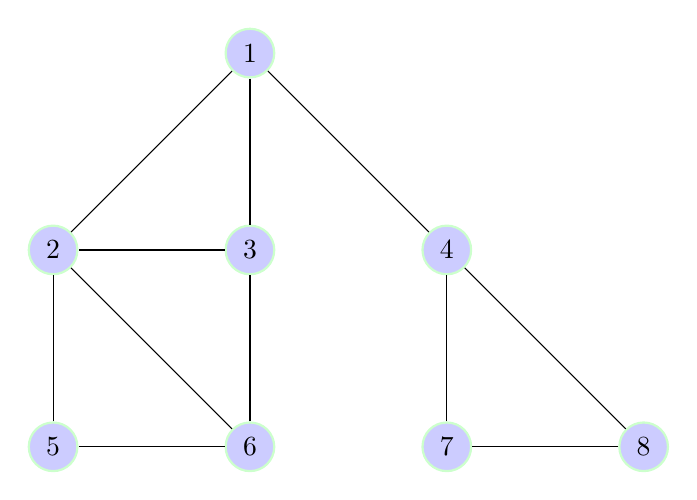
\begin{tikzpicture}{node distance=1.3cm,>=stealth',bend angle=45, auto}
        {

          \tikzstyle{place}=[circle,thick,draw=green!20,fill=blue!20,minimum size=6mm]
          \tikzstyle{texto}=[]
          \begin{scope}

            \node [place] (c1) {$2$};

            \node [place] (c2) [right of=c1,xshift=1.5cm] {$3$}
            edge [] (c1);

            \node [place] (c3) [above of=c2,yshift=1.5cm] {$1$}
            edge [] (c1)
            edge [] (c2);

            \node [place] (c4) [below of=c2,yshift=-1.5cm] {$6$}
            edge [] (c2)
            edge [] (c1);

            \node [place] (c5) [below of=c1,yshift=-1.5cm] {$5$}
            edge [] (c1)
            edge [] (c4);

            \node [place] (c6) [right of=c2,xshift=1.5cm] {$4$}
            edge [] (c3);

            \node [place] (c7) [below of=c6,yshift=-1.5cm] {$7$}
            edge [] (c6);

            \node [place] (c8) [right of=c7,xshift=1.5cm] {$8$}
            edge [] (c7)
            edge [] (c6);


          \end{scope}
        }
        \end{tikzpicture}
      \end{minipage}}
      \begin{center}
      \vspace{-2.5in}{\begin{minipage}{.05\columnwidth}%
        \centering%
        \begin{tikzpicture}{node distance=1.3cm,>=stealth',bend angle=45, auto}
          {

            \tikzstyle{place}=[circle,thick,draw=green!20,fill=blue!20,minimum size=6mm]
            \tikzstyle{texto}=[]
            \begin{scope}

              \node [place] (c1) [label=left:\textcolor{black}{$2$},label=right:\textcolor{black}{$1$}]{$2$};

              \node [texto] (c2) [right of=c1,xshift=1.5cm] {};

              \node [place] (c3) [above of=c2,yshift=1.5cm,label=right:\textcolor{black}{$1$},label=left:\textcolor{black}{$1$}] {$1$}
              edge [post] (c1);

              \node [place] (c4) [below of=c1,yshift=-.5cm,label=right:\textcolor{black}{$1$},label=left:\textcolor{black}{$3$}] {$3$}
              edge [pre] (c1)
              edge [bend right,dashed] (c3) ;

              \node [place] (c5) [below of=c4,yshift=-.5cm,label=right:\textcolor{black}{$2$},label=left:\textcolor{black}{$4$}] {$6$}
              edge [pre] (c4)
              edge [bend left=60,dashed] (c1) ;

              \node [place] (c6) [right of=c2,xshift=1.5cm,label=right:\textcolor{black}{$6$},label=left:\textcolor{black}{$6$}] {$4$}
              edge [pre] (c3);

              \node [place] (c7) [below of=c6,yshift=-.5cm,label=right:\textcolor{black}{$6$},label=left:\textcolor{black}{$7$}] {$7$}
              edge [pre] (c6);

              \node [place] (c8) [below of=c5,yshift=-.5cm,label=right:\textcolor{black}{$2$},label=left:\textcolor{black}{$5$}] {$5$}
              edge [pre] (c5)
              edge [bend left=65,dashed] (c1) ;

              \node [place] (c9) [below of=c7,yshift=-.5cm,label=right:\textcolor{black}{$6$},label=left:\textcolor{black}{$8$}] {$8$}
              edge [pre] (c7)
              edge [bend right=60,dashed] (c6) ;
            \end{scope}
          }
        \end{tikzpicture}
      \end{minipage}}
    \end{center}
  \end{figure}%
\end{center}%
\begin{figure}[H]
\caption{Un grafo no dirigido y su árbol de recorrido en profundidad.}
\end{figure}


\subsection{Búsqueda en anchura (Breadth-First Search)}

Cuando un recorrido en profundidad llega a un vértice $v$, intenta a continuación visitar algún vecino de $v$, después algún vecino del vecino, y así sucesivamente. Cuando un recorrido en anchura llega a algún vértice $v$, por otra parte, primero visita todos los vecinos de $v$. Sólo examina vértices más alejados después de haber hecho esto. A diferencia del recorrido en profundidad, el recorrido en anchura no es naturalmente recursivo.\\

Supongamos que queremos encontrar un camino más corto entre dos vértices específicos de un grafo - un camino que conecte a los vértices con la peculiaridad de que no exista otro camino con esos vértices y menos aristas. El método clásico para llevar a cabo esta tarea, llamado Búsqueda en Anchura (Breadth-First search), es también la base de numerosos algoritmos para el procesamiento de grafos. La Búsqueda en Profundidad nos ofrece poca ayuda en la resolución de este problema, ya que el orden en el que navega a través del grafo no tiene relación con el objetivo de encontrar los caminos más cortos. Por el contrario, la Búsqueda en Anchura se basa en este cometido. Para encontrar un camino más corto desde $v$ hasta $w$, que comenzará en $v$ hasta $w$ comprobando entre todos los vértices que podemos llegar siguiendo una de las aristas, luego de comprobar todos los vértices que se pueden recorrer de esos extremos y así sucesivamente.\\

Cuando llegamos a un punto de la búsqueda en el grafo en donde tenemos que atravesar más de una arista, se elige una y almacenamos las demás sin procesar para un análisis posterior. En la Búsqueda en Profundidad, se suele utilizar la inserción de elementos en una pila (que es gestionada por una función o estructura auxiliar a la función de búsqueda recursiva) para este propósito. Usando la regla LIFO que caracteriza a las pilas para explorar pasadizos o pasajes que estén muy próximos en un laberinto: Para ello elegimos, de las caminos que aún no hayan sido revisados, aquella que sea la más recientemente visitada. En la Búsqueda por Anchura, se explorarán los vértices según su ponderación o coste desde el punto de partida del camino o análisis. Para un laberinto, hacer esta búsqueda en este orden puede requerir un equipo entero de búsqueda; pero dentro de un programa de ordenador es más fácil de solucionar. Simplemente utilizaremos una estructura de tipo FIFO (cola) en lugar de una LIFO (pila).\\

\vfill
\pagebreak
\figuratikz{1}{Un árbol de búsqueda en anchura. Los nodos son numerados en el orden en que serán procesados por el algoritmo. El hijo de un nodo se visita de izquierda a derecha.}
{
  \tikzstyle{place}=[circle,thick,draw=green!20,fill=blue!20,minimum size=6mm]
  \tikzstyle{texto}=[]

  \begin{scope}

    \node [place] (c1) {$2$};

    \node [texto] (c2) [right of=c1,xshift=2.5cm] {};

    \node [place] (c3) [above of=c2,yshift=1.5cm] {$1$}
    edge [] (c1);

    \node [place] (c4) [below of=c1,yshift=-.5cm] {$6$}
    edge [] (c1);

    \node [place] (c6) [right of=c2,xshift=2.5cm] {$4$}
    edge [] (c3);

    \node [place] (c7) [below of=c6,yshift=-.5cm] {$11$}
    edge [] (c6);

    \node [place] (c10) [below of=c3,yshift=-1.5cm] {$3$}
    edge [] (c3);

    \node [place] (c11) [below of=c10,xshift=-.75cm,yshift=-.5cm] {$8$}
    edge [] (c10);

    \node [place] (c12) [below of=c10,xshift=.75cm,yshift=-.5cm] {$9$}
    edge [] (c10);

    \node [place] (c13) [left of=c4,xshift=-.25cm] {$5$}
    edge [] (c1);

    \node [place] (c14) [right of=c4,xshift=.25cm] {$7$}
    edge [] (c1);

    \node [place] (c15) [below of=c4,xshift=-.75cm,yshift=-.5cm] {$13$}
    edge [] (c4);

    \node [place] (c16) [below of=c4,xshift=.75cm,yshift=-.5cm] {$14$}
    edge [] (c4);

    \node [place] (c17) [below of=c7,xshift=-.75cm,yshift=-.5cm] {$15$}
    edge [] (c7);

    \node [place] (c17) [below of=c7,xshift=.75cm,yshift=-.5cm] {$16$}
    edge [] (c7);

  \end{scope}

}

\underline{Algoritmo de Búsqueda en Anchura}\\
\begin{Verbatim}[commandchars=\\\{\}]
\PY{c+cm}{/**}
\PY{c+cm}{ * Método observador.}
\PY{c+cm}{ * Muestra por la salida estándar el recorrido en anchura del grafo G.}
\PY{c+cm}{ * @param G matriz de adyacencia del grafo conexo.}
\PY{c+cm}{ */}

\PY{k+kd}{public} \PY{k+kt}{void} \PY{n+nf}{recorrido\PYZus{}anchura}\PY{o}{(}\PY{k+kt}{int} \PY{o}{[}\PY{o}{]}\PY{o}{[}\PY{o}{]} \PY{n}{G}\PY{o}{)} 
\PY{o}{\PYZob{}}
    \PY{k+kt}{int} \PY{n}{tama\PYZus{}G} \PY{o}{=} \PY{n}{G}\PY{o}{.}\PY{n+na}{length}\PY{o}{;}

    \PY{k+kt}{boolean} \PY{o}{[}\PY{o}{]} \PY{n}{marcas} \PY{o}{=} \PY{k}{new} \PY{k+kt}{boolean} \PY{o}{[}\PY{n}{tama\PYZus{}G}\PY{o}{]}\PY{o}{;}
    \PY{k+kt}{int} \PY{n}{i}\PY{o}{,}\PY{n}{v}\PY{o}{,}\PY{n}{w}\PY{o}{;} \PY{c+c1}{//Vértices.}

    \PY{n}{LinkedList}\PY{o}{<}\PY{n}{Integer}\PY{o}{>} \PY{n}{Cola} \PY{o}{=} \PY{k}{new} \PY{n}{LinkedList}\PY{o}{(}\PY{o}{)}\PY{o}{;}
    \PY{n}{rec\PYZus{}breadth} \PY{o}{=} \PY{k}{new} \PY{n}{ArrayList}\PY{o}{<}\PY{n}{Integer}\PY{o}{>}\PY{o}{(}\PY{o}{)}\PY{o}{;}

    \PY{n}{Arrays}\PY{o}{.}\PY{n+na}{fill}\PY{o}{(}\PY{n}{marcas}\PY{o}{,}\PY{l+m+mi}{0}\PY{o}{,}\PY{n}{tama\PYZus{}G}\PY{o}{,}\PY{k+kc}{false}\PY{o}{)}\PY{o}{;}
    \PY{n}{System}\PY{o}{.}\PY{n+na}{out}\PY{o}{.}\PY{n+na}{println}\PY{o}{(}\PY{l+s}{"REC\PYZus{}ANCHURA"}\PY{o}{)}\PY{o}{;}
    \PY{k}{for}\PY{o}{(}\PY{n}{i}\PY{o}{=}\PY{l+m+mi}{0}\PY{o}{;} \PY{n}{i} \PY{o}{<} \PY{n}{tama\PYZus{}G}\PY{o}{;} \PY{o}{+}\PY{o}{+}\PY{n}{i}\PY{o}{)}
	\PY{k}{if}\PY{o}{(}\PY{o}{!}\PY{n}{marcas}\PY{o}{[}\PY{n}{i}\PY{o}{]}\PY{o}{)} \PY{c+c1}{//NO visitado}
	    \PY{o}{\PYZob{}}
		\PY{n}{Cola}\PY{o}{.}\PY{n+na}{add}\PY{o}{(}\PY{n}{i}\PY{o}{)}\PY{o}{;} \PY{c+c1}{//Frente de la Cola}
		    
		\PY{k}{do}\PY{o}{\PYZob{}}
		    \PY{n}{v} \PY{o}{=} \PY{n}{Cola}\PY{o}{.}\PY{n+na}{getFirst}\PY{o}{(}\PY{o}{)}\PY{o}{;}
		    \PY{n}{Cola}\PY{o}{.}\PY{n+na}{removeFirst}\PY{o}{(}\PY{o}{)}\PY{o}{;} \PY{c+c1}{//Eliminamos el elemento.}
		    \PY{k}{if}\PY{o}{(}\PY{o}{!}\PY{n}{marcas}\PY{o}{[}\PY{n}{v}\PY{o}{]}\PY{o}{)} \PY{c+c1}{//NO visitado.}
			\PY{o}{\PYZob{}}
			    \PY{c+cm}{/* Marcar y procesar. */}
			    \PY{n}{marcas}\PY{o}{[}\PY{n}{v}\PY{o}{]} \PY{o}{=} \PY{k+kc}{true}\PY{o}{;} \PY{c+c1}{//Visitado.}
			    \PY{n}{System}\PY{o}{.}\PY{n+na}{out}\PY{o}{.}\PY{n+na}{print}\PY{o}{(}\PY{n}{v}\PY{o}{+}\PY{l+s}{" "}\PY{o}{)}\PY{o}{;}
			    \PY{n}{rec\PYZus{}breadth}\PY{o}{.}\PY{n+na}{add}\PY{o}{(}\PY{n}{v}\PY{o}{)}\PY{o}{;}
				
			    \PY{c+cm}{/* Encolar los adyacentes no visitados. */}

			    \PY{k}{for}\PY{o}{(}\PY{n}{w}\PY{o}{=}\PY{l+m+mi}{0}\PY{o}{;} \PY{n}{w} \PY{o}{<} \PY{n}{tama\PYZus{}G}\PY{o}{;} \PY{o}{+}\PY{o}{+}\PY{n}{w}\PY{o}{)}
				\PY{k}{if}\PY{o}{(}\PY{n}{G}\PY{o}{[}\PY{n}{v}\PY{o}{]}\PY{o}{[}\PY{n}{w}\PY{o}{]} \PY{o}{=}\PY{o}{=} \PY{l+m+mi}{1} \PY{o}{&}\PY{o}{&} \PY{n}{marcas}\PY{o}{[}\PY{n}{w}\PY{o}{]} \PY{o}{=}\PY{o}{=} \PY{k+kc}{false}\PY{o}{)}
				    \PY{n}{Cola}\PY{o}{.}\PY{n+na}{add}\PY{o}{(}\PY{n}{w}\PY{o}{)}\PY{o}{;}
			\PY{o}{\PYZcb{}}
		\PY{o}{\PYZcb{}}\PY{k}{while}\PY{o}{(}\PY{o}{!}\PY{o}{(}\PY{n}{Cola}\PY{o}{.}\PY{n+na}{isEmpty}\PY{o}{(}\PY{o}{)}\PY{o}{)}\PY{o}{)}\PY{o}{;}
	    \PY{o}{\PYZcb{}}
    \PY{n}{System}\PY{o}{.}\PY{n+na}{out}\PY{o}{.}\PY{n+na}{println}\PY{o}{(}\PY{l+s}{""}\PY{o}{)}\PY{o}{;}
\PY{o}{\PYZcb{}}
\end{Verbatim}


\section{Coloración}

En ocasiones, un problema se puede modelar distribuyendo los vértices o las aristas de un cierto grafo en paquetes distintos, de manera que vértices (o aristas, en su caso) de un mismo paquete no sean adyacentes (respectivamente, incidentes). Si se da un mismo color a los elementos de un mismo paquete, y se emplean colores distintos para cada paquete, se obtiene lo que se da en llamar un vértice (arista) coloración. La idea es encontrar el menor número de paquetes (esto es, colores), para distribuir los elementos (vértices o aristas, según sea el caso).\\

Un planteamiento general que se ajusta a esta circunstancia es el llamado \emph{problema de incompatibilidades}, que consta de ciertos elementos (modelados por los vértices de un grafo) y relaciones de incompatibilidad entre ellos (las cuales determinan las aristas del grafo). El grafo resultante se denomina \emph{grafo de incompatibilidades}. El distribuir los elementos en el menor número de agrupaciones posible de forma que elementos incompatibles no compartan una misma agrupación, se traduce al instante en conseguir una vértice coloración (i.e.\footnote{Del Latín i.e. ``id est'' Significado: ``Esto es'', ``Es decir''} una asignación de colores a los vértices de manera que vértices adyacentes tengan colores distintos).\\

Como ejemplo, se puede considerar el problema de diseñar un calendario a doble vuelta para una competición deportiva en forma de liguilla de $n$ equipos, en la que todos se han de enfrentar con todos dos veces. Este problema admite una primera simplificación, en la que basta diseñar un calendario a una sola vuelta, para reproducirlo en la segunda vuelta cambiando los papeles de los equipos que juegan como locales y como visitantes.\\

Si se modela el problema como el grafo $G$ cuyos vértices son los $n$ equipos y las aristas entre ellos representan los partidos, evidentemente se tiene que $G = K_n$, grafo completo de $n$ vértices. Organizar el calendario se traduce en repartir los partidos (aristas) en jornadas (colores), de manera que un mismo equipo (vértice) no juegue más de una vez en cada jornada (no aparezca como extremo en más de una arista). En definitiva, se trata de colorear las aristas de $K_n$ utilizando el menor número de colores, de manera que aristas con el mismo color representan partidos que se pueden jugar en la misma jornada.\\

Este problema admite ser modelado de otra forma: considérese el grafo $H$ cuyos vértices son los partidos a jugar, y cuyas aristas relacionan partidos incompatibles, en tanto en cuanto implican a un mismo equipo. Resolver el problema consiste ahora en encontrar una vértice coloración de $H$.\\

\subsection{Vértice coloraciones}

\begin{fondo}
Se denomina vértice coloración de un grafo $G = (V,A)$ a una asignación $c: V \rightarrow \mathbb{N}$ que asocie a cada vértice $x_i$ un color $c_i \in \mathbb{N}$, de manera que a vértices adyacentes correspondan colores distintos: si $\{x_i,x_j\} \in A$ entonces $c_i \ne c_j$. Si la coloración consta de una paleta de $k$ colores, entonces se habla simplemente de $k$-coloración.
\end{fondo}

Dado un grafo $G = (V,A)$, siempre existe un valor umbral $k$ para el cual $G$ admite una vértice coloración con una paleta de $k$ colores, pero no una $(k-1)$-coloración. Es decir, $k$ es el menor número de colores con los que se puede obtener una vértice coloración de $G$. Este valor se conoce como \emph{número cromático} de $G$, y se denota en la forma $\chi (G) = k$.\\

Determinar cuál es el número cromático de un grafo es en general un problema de una envergadura considerable: \textbf{no hay} un procedimiento que dé una respuesta en tiempo razonable, para un grafo genérico dado.\\

Ni que decir tiene que el número cromático de un grafo no conexo consiste en el mayor de entre los números cromáticos de sus componentes conexas, razón por la cual nos centraremos en el estudio de coloraciones sobres grafos conexos.\\

Con normalidad, se tiende a acotar el número cromático tanto inferior como superiormente, $s \leq \chi (G) \leq t$, de manera que progresivamente se afinan estas cotas hasta llevarlas a coincidir, $s = \chi (G) = t$, momento en el cual queda completamente determinado $\chi (G)$.\\

Sin mucho esfuerzo, es fácil asegurar de entrada que $1 \leq \chi (G) \leq v$ para grafos $G$ de $v$ vértices. Más aún, $\chi (G) = 1$ sólo en el caso de grafos $G$ vacíos, mientras que $\chi (G) = v$ en un grafo de $v$ vértices sólo si $G = K_v$.\\

El \textbf{teorema de Brooks} perfila un poco más la cota superior para $\chi (G)$ en grafos conexos, en función de la valencia (grado) máxima:
\[ \Delta =\ \mbox{max}_{x \in V}\ gr_G(x):
\left\{ 
\begin{array}{l}
\chi (K_n) = n = \Delta + 1\ \mbox{y}\ \chi (C_{2n + 1}) = 3 = \Delta + 1 \\
\mbox{En otro caso,}\ \chi (G) \leq \Delta
\end{array}
\right. \]

No obstante, esta cota puede ser bastante rudimentaria (piénsese en un grafo estrella $S_m$ de $m$ puntas, con $m = 1000$ por ejemplo: se tiene que $\chi (S_m) = 2$, mientras que $\Delta = m = 1000$).\\

Para obtener cotas inferiores, es frecuente buscar subgrafos $H \subseteq G$ de los cuales se conozca $\chi (H)$, toda vez que $\chi (H) \leq \chi (G)$ para cualquier $H \subseteq G$.\\

Para obtener cotas superiores, se suele realizar coloraciones concretas, de manera que $\chi (G)$ siempre es menor o igual que el número de colores utilizados.\\

A la hora de realizar coloraciones, es útil el llamado \emph{algoritmo voraz}, el cual, progresando sobre una ordenación prefijada de los vértices, procede a colorearlos asignando a cada vértice el primer color libre (i.e. el primer color no utilizado en los vértices a él adyacentes previamente coloreados).\\

Aunque este algoritmo no tiene por qué devolver el número cromático de $G$, con normalidad devuelve un número razonablemente pequeño de colores. No obstante, siempre se puede aplicar varias veces el algoritmo a ordenaciones distintas de los vértices, para ver si eventualmente el número de colores desciende. Una aplicación exhaustiva del algoritmo a las $V!$ ordenaciones posibles en un grafo de $V$ vértices resolvería efectivamente el problema; la ``única'' dificultad estriba en que $V!$ aplicaciones del algoritmo resultan ya impracticables cuando $V$ no es siquiera demasiado grande (nótese que $8! = 40320$).\\

\underline{Algoritmo de Vértice Coloración (Número Cromático)}\\
\begin{Verbatim}[commandchars=\\\{\}]
\PY{c+cm}{/**}
\PY{c+cm}{ * Método observador (Número cromático del grafo)}
\PY{c+cm}{ * @param G: matriz bidimensional de enteros que representa al grafo de}
\PY{c+cm}{ * trabajo actual.}
\PY{c+cm}{ * @return int que es el número cromático del grafo.}
\PY{c+cm}{ */}

\PY{k+kd}{public} \PY{k+kt}{int} \PY{n+nf}{k\PYZus{}colores}\PY{o}{(}\PY{k+kt}{int} \PY{o}{[}\PY{o}{]}\PY{o}{[}\PY{o}{]} \PY{n}{G}\PY{o}{)}
\PY{o}{\PYZob{}}
    \PY{k+kt}{int} \PY{n}{tama\PYZus{}G} \PY{o}{=} \PY{n}{G}\PY{o}{.}\PY{n+na}{length}\PY{o}{;}
    \PY{k+kt}{int} \PY{n}{elto}\PY{o}{=}\PY{l+m+mi}{0}\PY{o}{,} \PY{n}{original}\PY{o}{=}\PY{l+m+mi}{0}\PY{o}{;}
    \PY{k+kt}{int} \PY{o}{[}\PY{o}{]} \PY{n}{color} \PY{o}{=} \PY{k}{new} \PY{k+kt}{int} \PY{o}{[}\PY{n}{tama\PYZus{}G}\PY{o}{]}\PY{o}{;}
    \PY{n}{Arrays}\PY{o}{.}\PY{n+na}{fill}\PY{o}{(}\PY{n}{color}\PY{o}{,}\PY{l+m+mi}{0}\PY{o}{)}\PY{o}{;} \PY{c+c1}{//Rellenamos con el color vacío todo el vector.}
    \PY{k+kt}{int} \PY{n}{i}\PY{o}{;}
    \PY{k+kt}{boolean} \PY{n}{salto}\PY{o}{=}\PY{k+kc}{false}\PY{o}{;}


    \PY{n}{HashMap}\PY{o}{<}\PY{n}{Integer}\PY{o}{,}\PY{n}{ArrayList}\PY{o}{<}\PY{n}{Integer}\PY{o}{>}\PY{o}{>}  \PY{n}{v\PYZus{}ady} 
	\PY{o}{=} \PY{k}{new} \PY{n}{HashMap}\PY{o}{<}\PY{n}{Integer}\PY{o}{,}\PY{n}{ArrayList}\PY{o}{<}\PY{n}{Integer}\PY{o}{>}\PY{o}{>}\PY{o}{(}\PY{o}{)}\PY{o}{;}
    \PY{n}{ArrayList}\PY{o}{<}\PY{n}{Integer}\PY{o}{>} \PY{n}{ady}\PY{o}{;}


    \PY{k}{for}\PY{o}{(}\PY{n}{i}\PY{o}{=}\PY{l+m+mi}{0}\PY{o}{;} \PY{n}{i} \PY{o}{<} \PY{n}{tama\PYZus{}G}\PY{o}{;} \PY{o}{+}\PY{o}{+}\PY{n}{i}\PY{o}{)}
	\PY{o}{\PYZob{}}
	    \PY{n}{ady} \PY{o}{=} \PY{k}{new} \PY{n}{ArrayList}\PY{o}{<}\PY{n}{Integer}\PY{o}{>}\PY{o}{(}\PY{o}{)}\PY{o}{;}

	    \PY{k}{for}\PY{o}{(}\PY{k+kt}{int} \PY{n}{j}\PY{o}{=}\PY{l+m+mi}{0}\PY{o}{;} \PY{n}{j} \PY{o}{<} \PY{n}{tama\PYZus{}G}\PY{o}{;} \PY{o}{+}\PY{o}{+}\PY{n}{j}\PY{o}{)}
		\PY{o}{\PYZob{}}
		    \PY{k}{if}\PY{o}{(}\PY{n}{G}\PY{o}{[}\PY{n}{i}\PY{o}{]}\PY{o}{[}\PY{n}{j}\PY{o}{]} \PY{o}{!}\PY{o}{=} \PY{l+m+mi}{0}\PY{o}{)}
			\PY{o}{\PYZob{}}
			    \PY{n}{ady}\PY{o}{.}\PY{n+na}{add}\PY{o}{(}\PY{n}{j}\PY{o}{)}\PY{o}{;}
			\PY{o}{\PYZcb{}}
		\PY{o}{\PYZcb{}}

	    \PY{n}{v\PYZus{}ady}\PY{o}{.}\PY{n+na}{put}\PY{o}{(}\PY{n}{i}\PY{o}{,}\PY{n}{ady}\PY{o}{)}\PY{o}{;}
	\PY{o}{\PYZcb{}}

    \PY{n}{i}\PY{o}{=}\PY{l+m+mi}{0}\PY{o}{;}
    \PY{k+kt}{int} \PY{n}{z}\PY{o}{=}\PY{l+m+mi}{0}\PY{o}{;}
    \PY{k}{while}\PY{o}{(}\PY{n}{i} \PY{o}{<} \PY{n}{tama\PYZus{}G}\PY{o}{)}
	\PY{o}{\PYZob{}}
	    \PY{n}{z} \PY{o}{=} \PY{n}{rec\PYZus{}depth}\PY{o}{.}\PY{n+na}{get}\PY{o}{(}\PY{n}{i}\PY{o}{)}\PY{o}{;}
	    \PY{n}{color}\PY{o}{[}\PY{n}{z}\PY{o}{]} \PY{o}{+}\PY{o}{=} \PY{l+m+mi}{1}\PY{o}{;}
	    \PY{n}{original} \PY{o}{=} \PY{n}{color}\PY{o}{[}\PY{n}{z}\PY{o}{]}\PY{o}{;}

	    \PY{k}{for}\PY{o}{(}\PY{k+kt}{int} \PY{n}{j}\PY{o}{=}\PY{l+m+mi}{0}\PY{o}{;} \PY{n}{j} \PY{o}{<} \PY{n}{v\PYZus{}ady}\PY{o}{.}\PY{n+na}{get}\PY{o}{(}\PY{n}{z}\PY{o}{)}\PY{o}{.}\PY{n+na}{size}\PY{o}{(}\PY{o}{)} \PY{o}{&}\PY{o}{&} \PY{o}{!}\PY{n}{salto}\PY{o}{;} \PY{o}{+}\PY{o}{+}\PY{n}{j}\PY{o}{)}
		\PY{o}{\PYZob{}}
		    \PY{n}{elto} \PY{o}{=} \PY{n}{v\PYZus{}ady}\PY{o}{.}\PY{n+na}{get}\PY{o}{(}\PY{n}{z}\PY{o}{)}\PY{o}{.}\PY{n+na}{get}\PY{o}{(}\PY{n}{j}\PY{o}{)}\PY{o}{;}
		    \PY{k}{if}\PY{o}{(}\PY{n}{color}\PY{o}{[}\PY{n}{elto}\PY{o}{]} \PY{o}{=}\PY{o}{=} \PY{n}{color}\PY{o}{[}\PY{n}{z}\PY{o}{]}\PY{o}{)}
			\PY{o}{\PYZob{}}
			    \PY{n}{color}\PY{o}{[}\PY{n}{z}\PY{o}{]} \PY{o}{+}\PY{o}{=} \PY{l+m+mi}{1}\PY{o}{;}
			    \PY{n}{salto} \PY{o}{=} \PY{k+kc}{true}\PY{o}{;}
			\PY{o}{\PYZcb{}}
		\PY{o}{\PYZcb{}}

       
	    \PY{k}{if}\PY{o}{(}\PY{n}{original} \PY{o}{=}\PY{o}{=} \PY{n}{color}\PY{o}{[}\PY{n}{z}\PY{o}{]}\PY{o}{)}
		\PY{n}{i}\PY{o}{+}\PY{o}{+}\PY{o}{;}
	    \PY{k}{else}
		\PY{n}{i}\PY{o}{=}\PY{l+m+mi}{0}\PY{o}{;}
	\PY{o}{\PYZcb{}} 

    \PY{n}{elto} \PY{o}{=} \PY{n}{color}\PY{o}{[}\PY{l+m+mi}{0}\PY{o}{]}\PY{o}{;}
	
    \PY{k}{for}\PY{o}{(}\PY{n}{i}\PY{o}{=}\PY{l+m+mi}{0}\PY{o}{;} \PY{n}{i} \PY{o}{<} \PY{n}{tama\PYZus{}G}\PY{o}{;} \PY{o}{+}\PY{o}{+}\PY{n}{i}\PY{o}{)}
	\PY{k}{if}\PY{o}{(}\PY{n}{color}\PY{o}{[}\PY{n}{i}\PY{o}{]} \PY{o}{>} \PY{n}{elto}\PY{o}{)}
	    \PY{n}{elto} \PY{o}{=} \PY{n}{color}\PY{o}{[}\PY{n}{i}\PY{o}{]}\PY{o}{;}

    \PY{k}{return} \PY{n}{elto}\PY{o}{;}

	
\PY{o}{\PYZcb{}}
\end{Verbatim}


\section{Ordenación topológica}

La Ordenación Topológica es la operación más importante en los grafos acíclicos dirigidos (DAG). Este ordena los vértices en una línea de tal manera que todas las aristas dirigidas vayan de izquierda a derecha. Tal ordenamiento no puede existir si el grafo contiene un ciclo dirigido.\\

Cada DAG tiene al menos una ordenación topológica. La importancia de la ordenación topológica es que ordena procesando cada vértice antes de cualquier sucesor que tenga. Supongamos que las aristas representan restricciones de prioridad, de modo que la arista $(x,y)$ significa que el trabajo o proceso $x$ debe hacerse antes del proceso $y$. Entonces, cualquier ordenación topológica define un programa de forma lícita. De hecho, puede haber muchas ordenaciones para un mismo DAG dado.\\

\figuratikz{1}{Un DAG con un solo orden topológico $(G,A,B,C,F,E,D)$}
{
  \tikzstyle{place}=[circle,thick,draw=green!20,fill=blue!20,minimum size=4mm]

  \begin{scope}

    \node [place] (c1) [label=left:\textcolor{black}{$A$}] {};

    \node [place] (c2) [below of=c1,yshift=-1cm,label=left:\textcolor{black}{$G$}] {}
    edge [post] (c1);

    \node [place] (c3) [right of=c1,xshift=.5cm,yshift=.5cm,label=above:\textcolor{black}{$B$}] {}
    edge [pre] (c1);

    \node [place] (c4) [below of=c3,yshift=-.2cm,xshift=.4cm,label=below:\textcolor{black}{$C$}] {}
    edge [pre] (c3)
    edge [pre] (c1);

    \node [place] (c5) [right of=c2,xshift=3cm,label=right:\textcolor{black}{$F$}] {}
    edge [pre] (c2)
    edge [pre] (c4);

    \node [place] (c6) [right of=c4,xshift=1cm,yshift=.3cm,label=right:\textcolor{black}{$E$}] {}
    edge [pre] (c4)
    edge [pre] (c5);

    \node [place] (c7) [right of=c6,xshift=.4cm,yshift=.8cm,label=above:\textcolor{black}{$D$}] {}
    edge [pre] (c3)
    edge [pre] (c6);


  \end{scope}

}

Pero las aplicaciones son más variadas. Supongamos que buscamos el camino más corto (o largo) desde $x$ a $y$ en un DAG. Ningún vértice aparece después de $y$ en el orden topológico que puede contribuir a cualquiera de estos caminos, porque no habrá forma de volver a $y$. Podríamos procesar de forma correcta todos los vértices desde la izquierda a la derecha en el orden topológico, considerando el impacto de sus aristas exteriores, y sabiendo que se han analizado todo antes de que se necesite en otra operación. El orden topológico resulta muy útil para prácticamente cualquier problema algorítmico en grafos dirigidos.\\

El orden topológico puede realizarse de una manera eficiente usando la búsqueda en profundidad. Un grafo dirigido es un DAG si y sólo si no hay aristas de retroceso en él. Etiquetando los vértices en el orden inverso al que fueron procesados se encuentra una ordenación topológica de un DAG. ¿Porqué? Considere que sucede con cada arista dirigida $\{x,y\}$ cuando nos encontramos explorando el vértice $x$:\\

\begin{itemize}
\item Si no se ha pasado por $y$ aún, entonces comenzaremos una búsqueda en profundidad en $y$ antes de que podamos continuar con $x$. Por lo tanto, $y$ es marcado como "procesado" antes que $x$ lo sea, y $x$ aparece antes que $y$ en la ordenación topológica, como debería ser.
\item Si se ha pasado por $y$ pero no se ha marcado como "procesado", entonces $\{x,y\}$ es una arista de retroceso, lo cual no estaría permitido en un DAG.
\item Si $y$ se ha procesado, entonces habrá sido etiquetado antes que $x$. De tal forma que, $x$ aparece antes que $y$ en el orden topológico, como debería ser
\end{itemize}

\underline{Algoritmo de Ordenación Topológica}\\
\begin{Verbatim}[commandchars=\\\{\}]
\PY{c+cm}{/**}
\PY{c+cm}{ * Método modificador }
\PY{c+cm}{ * Realiza la ordenación topológica del grafo de trabajo y la muestra}
\PY{c+cm}{ * por el flujo de salida estándar.}
\PY{c+cm}{ * @param G: matriz bidimensional de enteros cuyo contenido es el grafo}
\PY{c+cm}{ * de trabajo actual.}
\PY{c+cm}{ */}

\PY{k+kd}{public} \PY{k+kt}{void} \PY{n+nf}{ordenacion\PYZus{}topologica}\PY{o}{(}\PY{k+kt}{int} \PY{o}{[}\PY{o}{]}\PY{o}{[}\PY{o}{]} \PY{n}{G}\PY{o}{)}
\PY{o}{\PYZob{}}
    \PY{n}{System}\PY{o}{.}\PY{n+na}{out}\PY{o}{.}\PY{n+na}{println}\PY{o}{(}\PY{l+s}{"ORDENACION TOPOLOGICA"}\PY{o}{)}\PY{o}{;}
	
    \PY{k+kt}{int} \PY{n}{tama\PYZus{}G} \PY{o}{=} \PY{n}{G}\PY{o}{.}\PY{n+na}{length}\PY{o}{;}
    \PY{n}{vertice\PYZus{}visitado} \PY{o}{=} \PY{k}{new} \PY{k+kt}{boolean} \PY{o}{[}\PY{n}{tama\PYZus{}G}\PY{o}{]}\PY{o}{;}
    \PY{n}{pila} \PY{o}{=} \PY{k}{new} \PY{n}{Stack}\PY{o}{<}\PY{n}{Integer}\PY{o}{>}\PY{o}{(}\PY{o}{)}\PY{o}{;}

    \PY{k}{for}\PY{o}{(}\PY{k+kt}{int} \PY{n}{i}\PY{o}{=}\PY{l+m+mi}{0}\PY{o}{;} \PY{n}{i} \PY{o}{<} \PY{n}{tama\PYZus{}G}\PY{o}{;} \PY{o}{+}\PY{o}{+}\PY{n}{i}\PY{o}{)}
	\PY{n}{vertice\PYZus{}visitado}\PY{o}{[}\PY{n}{i}\PY{o}{]} \PY{o}{=} \PY{k+kc}{true}\PY{o}{;}

    \PY{k}{for}\PY{o}{(}\PY{k+kt}{int} \PY{n}{i}\PY{o}{=}\PY{l+m+mi}{0}\PY{o}{;} \PY{n}{i} \PY{o}{<} \PY{n}{tama\PYZus{}G}\PY{o}{;} \PY{o}{+}\PY{o}{+}\PY{n}{i}\PY{o}{)}
	\PY{k}{if}\PY{o}{(}\PY{n}{vertice\PYZus{}visitado}\PY{o}{[}\PY{n}{i}\PY{o}{]}\PY{o}{)}
	    \PY{n}{topolog\PYZus{}rec}\PY{o}{(}\PY{n}{i}\PY{o}{,}\PY{n}{G}\PY{o}{)}\PY{o}{;}

    \PY{n}{Stack}\PY{o}{<}\PY{n}{Integer}\PY{o}{>} \PY{n}{salida} \PY{o}{=} \PY{k}{new} \PY{n}{Stack}\PY{o}{<}\PY{n}{Integer}\PY{o}{>}\PY{o}{(}\PY{o}{)}\PY{o}{;}

    \PY{k}{while}\PY{o}{(}\PY{o}{!}\PY{n}{pila}\PY{o}{.}\PY{n+na}{empty}\PY{o}{(}\PY{o}{)}\PY{o}{)}
	\PY{o}{\PYZob{}}
	    \PY{n}{salida}\PY{o}{.}\PY{n+na}{push}\PY{o}{(}\PY{n}{pila}\PY{o}{.}\PY{n+na}{peek}\PY{o}{(}\PY{o}{)}\PY{o}{)}\PY{o}{;}
	    \PY{n}{pila}\PY{o}{.}\PY{n+na}{pop}\PY{o}{(}\PY{o}{)}\PY{o}{;}
	\PY{o}{\PYZcb{}}

    \PY{n}{System}\PY{o}{.}\PY{n+na}{out}\PY{o}{.}\PY{n+na}{print}\PY{o}{(}\PY{l+s}{"("}\PY{o}{)}\PY{o}{;}
    \PY{k}{while}\PY{o}{(}\PY{o}{!}\PY{n}{salida}\PY{o}{.}\PY{n+na}{empty}\PY{o}{(}\PY{o}{)}\PY{o}{)}
	\PY{o}{\PYZob{}}
	    \PY{n}{System}\PY{o}{.}\PY{n+na}{out}\PY{o}{.}\PY{n+na}{print}\PY{o}{(}\PY{l+s}{" "}\PY{o}{+}\PY{n}{salida}\PY{o}{.}\PY{n+na}{peek}\PY{o}{(}\PY{o}{)}\PY{o}{)}\PY{o}{;}
	    \PY{n}{salida}\PY{o}{.}\PY{n+na}{pop}\PY{o}{(}\PY{o}{)}\PY{o}{;}
	\PY{o}{\PYZcb{}}
    \PY{n}{System}\PY{o}{.}\PY{n+na}{out}\PY{o}{.}\PY{n+na}{println}\PY{o}{(}\PY{l+s}{" )"}\PY{o}{)}\PY{o}{;}
\PY{o}{\PYZcb{}}

\PY{c+cm}{/**}
\PY{c+cm}{ * Método observador. (privado)}
\PY{c+cm}{ * Es la función auxiliar que ayuda a procesar el orden topológico}
\PY{c+cm}{ * para el grafo actual.}
\PY{c+cm}{ * @param G: matriz bidimensional de enteros cuyo contenido es el grafo}
\PY{c+cm}{ * de trabajo actual.}
\PY{c+cm}{ * @param vertice: valor entero que representa un nodo del grafo G.}
\PY{c+cm}{ */}

\PY{k+kd}{private} \PY{k+kt}{void} \PY{n+nf}{topolog\PYZus{}rec}\PY{o}{(}\PY{k+kt}{int} \PY{n}{vertice}\PY{o}{,} \PY{k+kt}{int} \PY{o}{[}\PY{o}{]}\PY{o}{[}\PY{o}{]} \PY{n}{G}\PY{o}{)}
\PY{o}{\PYZob{}}
    \PY{n}{vertice\PYZus{}visitado}\PY{o}{[}\PY{n}{vertice}\PY{o}{]} \PY{o}{=} \PY{k+kc}{false}\PY{o}{;}
    \PY{k+kt}{int} \PY{n}{tama\PYZus{}G} \PY{o}{=} \PY{n}{G}\PY{o}{.}\PY{n+na}{length}\PY{o}{;}

    \PY{k}{for}\PY{o}{(}\PY{k+kt}{int} \PY{n}{i}\PY{o}{=}\PY{l+m+mi}{0}\PY{o}{;} \PY{n}{i} \PY{o}{<} \PY{n}{tama\PYZus{}G}\PY{o}{;} \PY{o}{+}\PY{o}{+}\PY{n}{i}\PY{o}{)}
	\PY{k}{if}\PY{o}{(}\PY{n}{G}\PY{o}{[}\PY{n}{i}\PY{o}{]}\PY{o}{[}\PY{n}{vertice}\PY{o}{]} \PY{o}{!}\PY{o}{=} \PY{l+m+mi}{0}\PY{o}{)}
	    \PY{k}{if}\PY{o}{(}\PY{n}{vertice\PYZus{}visitado}\PY{o}{[}\PY{n}{i}\PY{o}{]}\PY{o}{)}
		\PY{n}{topolog\PYZus{}rec}\PY{o}{(}\PY{n}{i}\PY{o}{,}\PY{n}{G}\PY{o}{)}\PY{o}{;}

    \PY{n}{pila}\PY{o}{.}\PY{n+na}{push}\PY{o}{(}\PY{n}{vertice}\PY{o}{)}\PY{o}{;}
\PY{o}{\PYZcb{}}
\end{Verbatim}



\chapter{La complejidad algorítmica}
\label{chap:notacion-asintotica}

Cuando tenemos que resolver un problema, es posible que estén disponibles varios algoritmos adecuados. Evidentemente, desearíamos seleccionar el mejor. Esto plantea la pregunta de cómo decidir entre varios algoritmos cuál es preferible. Si solamente tenemos que resolver uno o dos casos pequeños de un problema más bien sencillo, quizá no nos importe demasiado qué algoritmo utilizaremos: en este caso podríamos decidirnos a seleccionar sencillamente el que sea más fácil de programar, o uno para el cual ya exista un programa, sin preocuparnos por sus propiedades teóricas. Sin embargo, si tenemos que resolver muchos casos, o si el problema es difícil, quizá tengamos que seleccionar de forma más cuidadosa.\\

El enfoque \emph{empírico} (o a posteriori) para seleccionar un algoritmo consiste en programar las técnicas competidoras e ir probándolas en distintos casos con ayuda de una computadora. El enfoque \emph{teórico} (a priori) que es el que casi siempre se toma como referencia, consiste en determinar matemáticamente la cantidad de recursos necesarios para cada uno de los algoritmos \emph{como función del tamaño de los casos considerados}. Los recursos que más nos interesan son el tiempo de computación y el espacio de almacenamiento, siendo el primero normalmente el más importante. \\

El \emph{tamaño} de un ejemplar se corresponde formalmente con el número de \emph{bits} que se necesitan para representar el ejemplar en una computadora, utilizando algún esquema de codificación precisamente definido y razonablemente compacto. Sin embargo, para hacer más claros nuestros análisis, lo normal será que seamos menos formales, y utilizaremos la palabra ``tamaño'' para indicar cualquier entero que mida de alguna forma el número de componentes de un ejemplar. Por ejemplo, cuando estamos hablando acerca de ordenaciones, mediremos normalmente el tamaño de un ejemplar por el número de items que hay que ordenar ignorando el hecho consistente en que cada uno de estos items ocuparía más de un bit para representarlo en una computadora. De manera similar, cuando hablemos acerca de grafos, mediremos normalmente el tamaño de un ejemplar por el número de nodos o de aristas (o de ambos) implicados. Apartándonos un poco de esta regla general, sin embargo, cuando hablemos acerca de problemas que impliquen enteros, daremos algunas veces la eficiencia de nuestros algoritmos en términos del \emph{valor} del ejemplar que estemos considerando, en lugar de considerar su tamaño (que sería el número de bits \emph{bits} necesarios para representar en binario este valor).\\

La ventaja de la aproximación teórica es que no depende ni de la computadora que se esté utilizando, ni del lenguaje de programación, ni siquiera de las habilidades del programador. Se ahorra tanto el tiempo que se habría invertido innecesariamente para programar un algoritmo ineficiente, como el tiempo de máquina que se habría desperdiciado comprobándolo. Lo que es más significativo, se nos permite estudiar la eficiencia del algoritmo cuando se utiliza en casos de todos los tamaños. Esto no suele suceder con la aproximación empírica, en la cual las consideraciones prácticas podrían obligarnos a comprobar los algoritmos sólo en un pequeño número de ejemplares arbitrariamente seleccionados y de tamaño moderado. Dado que suele suceder que los algoritmos recién descubiertos empiezan a comportarse mejor que sus predecesores sólo cuando ambos se utilizan en ejemplares grandes, este último punto resulta especialmente importante. \\

Si deseamos medir la cantidad de espacio que utiliza un algoritmo en función del tamaño de los ejemplares, está a nuestra disposición una unidad natural, a saber, el \emph{bit}. Independientemente de la máquina que se esté utilizando, la noción de un \emph{bit} de almacenamiento está bien definida. Si, por otra parte, tal como suele suceder, deseamos medir la eficiencia de un algoritmo, en términos del tiempo que se necesita para llegar a una respuesta, entonces no existe una opción tan evidente. Está claro que no se puede pensar en expresar esta eficiencia, digamos, en segundos, puesto que no se dispone de una computadora estándar a la cual se pudieran referir todas las medidas (existe una computadora estándar, pero es un modelo teórico: la maquina de Turing).\\

Una respuesta a este problema es la que viene dada por el \emph{principio de invariancia}, que afirma que dos implementaciones distintas de un mismo algoritmo no diferirán en su eficiencia en más de alguna constante multiplicativa. Si esta constante fuera, por ejemplo, cinco, entonces sabemos que si la primera implementación requiere un segundo para resolver casos de un cierto tamaño, entonces la segunda implementación (quizá en una máquina distinta, o escrita en un lenguaje de programación distinto) no requerirá más de 5 segundos para resolver los mismos casos. Para ser más exactos, si dos implementaciones del mismo algoritmo necesitan $t_1(n)$ y $t_2(n)$ segundos, respectivamente, para resolver un caso de tamaño $n$, entonces siempre existen constantes positivas $c$ y $d$ tales que $t_1(n) \leq ct_2(n)$ y $t_2(n) \leq dt_1(n)$ siempre que $n$ sea lo suficientemente grande. En otras palabras, el tiempo de ejecución de cualquiera de las implementaciones está acotado por un múltiplo constante del tiempo de ejecución de la otra; la decisión de a qué implementación llamaremos primera, y a cuál llamaremos segunda, es irrelevante. La condición de que $n$ sea suficientemente grande no es realmente necesaria, según la \textbf{regla del umbral}:\\

\begin{fondo}
Una función $t_n$ pertenece al orden de $f(n):\ O(f(n))$
\begin{itemize}
\item cuando está acotada superiormente por $f(n)$ para valores de $n$ suficientemente grandes y
\item haciendo abstracción de posibles constantes multiplicativas
\end{itemize}
\begin{center}
\[O(f(n)) = \Bigl\{ t: \mathbb{N} \rightarrow \mathbb{R}^{\geq 0} \Bigl| \exists\ c \in \mathbb{R}^{+} , \exists n_{0} \in \mathbb{N} \Bigl| \forall n \geq n_{0} : t(n) \leq c \cdot f(n) \Bigl\} \]
\end{center}

\end{fondo}

Sin embargo, al incluirla suele ser posible hallar constantes más pequeñas $c$ y $d$ que las que se hallarían en caso contrario. Esto resulta útil si estamos intentando calcular buenas cotas acerca del tiempo de ejecución de una implementación cuando conocemos el tiempo de ejecución de la otra.\\

Volviendo a la cuestión de la unidad que se debe utilizar para expresar la eficiencia teórica de un algoritmo, el principio de invariancia nos permite decidir que no va a existir tal unidad. En su lugar, expresaremos solamente el tiempo requerido por el algoritmo salvo una constante multiplicativa. Diremos que un algoritmo para algún problema requiere un tiempo del orden de $t(n)$ para una función dada $t$, si existe una constante positiva $c$ y una implementación del algoritmo capaz de resolver todos los casos de tamaño $n$ en un tiempo que no sea superior a $ct(n)$ segundos. \\

El uso de segundos en esta definición es evidentemente arbitrario: sólo se necesita modificar la constante para acotar el tiempo por $at(n)$ años o por $bt(n)$ microsegundos. Por el principio de invariancia, si cualquier implementación del algoritmo tiene la propiedad requerida, entonces también la tienen todas las demás, aunque la constante multiplicativa pueda cambiar de una implementación a otra.\\

\section{Notación asintótica}

Esta notación se denomina ``asintótica'' porque trata acerca del comportamiento de funciones en el límite, esto es, para valores suficientemente grandes de su parámetro. En consecuencia, los argumentos basados en la notación asintótica pueden no llegar a tener un valor práctico cuando el parámetro adopta valores ``de la vida real''. Sin embargo, en las enseñanzas de la notación asintótica suelen tener una relevancia significativa. Esto se debe a que, un algoritmo que sea superior asintóticamente suele ser (aunque no siempre) preferible incluso en casos de tamaño moderado.\\

\subsection{La $O$ mayúscula}

Sea $t: \mathbb{N} \rightarrow \mathbb{R}^{\geq 0}$ una función arbitraria de los números naturales en los números reales no negativos, tal como $t(n) = 5n^2 + \frac{100}{3}n + 2$. Se suele pensar que $n$ representa el tamaño del ejemplar sobre el cual es preciso que se aplique un algoritmo dado, y en $t(n)$ como representante de la cantidad de un recurso dado que se invierte en ese ejemplar por una implementación particular de este algoritmo. Por ejemplo, podría ser que la implementación invirtiera $t(n)$ microsegundos en el ejemplar peor en un caso de tamaño $n$, o quizá $t(n)$ represente la cantidad de espacio. Tal como se ha visto, la función $t(n)$ puede muy bien depender de la implementación más que depender únicamente del algoritmo. Recuerde sin embargo el principio de invariancia, que dice que la \emph{razón} de los tiempos de ejecución de dos implementaciones diferentes del mismo algoritmo siempre está acotada por encima y por debajo mediante constantes predeterminadas. (Las constantes pueden depender de las implementaciones pero no del tamaño del ejemplar).\\

Considérese ahora una función $f: \\mathbb{N} \rightarrow \mathbb{R}^{\geq 0}$ tal como $f(n) = n^2$. Diremos que $t(n)$ está en el \emph{orden de f(n)} si $t(n)$ está acotada superiormente por un múltiplo real positivo de $f(n)$ para todo $n$ suficientemente grande. Matemáticamente, esto significa que existe una constante real y positiva $c$ y un entero umbral $n_0$ tal que $t(n) \leq cf(n)$, siempre que $n \geq n_0$.\\

Por ejemplo, considérese las funciones $f(n)$ y $t(n)$ definidas anteriormente. Está claro que tanto $n \leq n^2$ como $1 \leq n^2$, siempre que $n \geq 1$. Por tanto, siempre y cuando $n \geq 1$:

\begin{center}
\[ t(n) = 5n^2 + \frac{100}{3}n + 2 \]
\[ \geq 5n^2 + \frac{100}{3}n^2 + 2n^2 \]
\[ = 40n^2 = 40 f(n) \]
\end{center}

Tomando $c = 40$ (o cualquier valor mayor) y $n_0 = 1$, concluiremos por tanto que $t(n)$ es del orden de $f(n)$ por cuanto $t(n) \leq cf(n)$ siempre que $n \geq n_0$. Por tanto es conveniente disponer de un símbolo matemático para representar \emph{el orden de}. Una vez más sea $f: \mathbb{N} \rightarrow \mathbb{R}^{\geq 0}$ una función arbitraria de los números naturales en los reales no negativos. Le indicará mediante $O(f(n))$ - que se lee ``$O$ de $f(n)$'' - \emph{el conjunto} de todas las funciones $t: \mathbb{N} \rightarrow \mathbb{R}^{\geq 0}$ tales que $t(n) \leq cf(n)$ para todo $n \geq n_0$ para una constante positiva real $c$ y para un umbral entero $n_0$. En otras palabras:
\begin{center}
\[ O(f(n)) = \big\{ t: \mathbb{N} \rightarrow \mathbb{R}^{\geq 0} \big| \exists c \in \mathbb{R}^+\ \exists n_0 \in \mathbb{N}\ \forall n \geq n_0\ [t(n) \leq cf(n)] \big\} \]\\
\end{center}

\begin{nota}
A partir de ahora la notación del término $O(f(n))$ será $O(f)$ empleada en otros libros o referencias para facilitar su uso al lector. Igualmente la notación para la función $f(n)$ se sustituirá con la notación simple de $f$ siempre que no haya confusión.\\
\end{nota}

La notación $O(f)$, denota al conjunto de las funciones de $t$ que crecen a lo más tan rápido como $f$, es decir, las funciones $t$ tales que, mediante una \emph{constante multiplicativa}, $f$ llega a ser en algún momento una cota superior para $t$. Así pues la correspondencia con la definición es intuitiva: el cuantificador existencial sobre $c$ formaliza la expresión \emph{constantes multiplicativas}, y $n_0$ indica a partir de qué punto $f$ es realmente una cota superior para $t$.\\

A modo de ejemplo, aplicando la definición puede comprobarse que para $f(n) = n^2$ y $t(n) = n$ se tiene que $t \in O(f))$ pero sin embargo $f \notin O(t)$. Para $f(n) = 3n^2$ y $t(n) = 100n^2$ se tiene que $t \in O(f)$ y $f \in O(t)$.\\

La notación $O(f)$ tiene las siguientes propiedades, cualesquiera que sean las funciones $f,t$ y $g$.\\
\begin{enumerate}
\item \emph{Invariancia multiplicativa}. Para toda constante $c \in \mathbb{R}^+$,
\[ t \in O(f) \iff c \cdot t \in O(f) \]
Se demuestra por simple aplicación de la definición.
\item \emph{Reflexividad}. $f \in O(f)$. Basta comprobar la definición.
\item \emph{Transitividad}. Si $g \in O(t)$ y $t \in O(f)$ entonces $g \in O(f)$. Se demuestra mediante sencillas manipulaciones aritméticas.
\item \emph{Criterio de caracterización}. $t \in O(f) \iff O(t) \subseteq O(f)$. Se deduce fácilmente de las dos anteriores.
\item \emph{Regla de la suma para $O$}. $O(f+t) = O(max(f,t))$, donde denotamos $f+t$ la función que sobre el argumento $n$ vale $f(n)+t(n)$, y $max(f,t)$ la función sobre la que el argumento $n$ vale el máximo de $\{f(n),t(n)\}$. Frecuentemente esta regla se aplica así: si $t_1 \in O(f_1)$ y $t_2 \in O(f_2)$, entonces $t_1 + t_2 \in O(max(f_1,f_2))$.
\item \emph{Regla del producto para $O$}. Si $t_1 \in O(f_1)$ y $t_2 \in O(f_2)$, entonces $t_1 \cdot t_2 \in O(f_1 \cdot f_2)$, donde denotamos $f \cdot t$ la función que sobre el argumento $n$ vale $f(n) \cdot t(n)$.
\item \emph{Invariancia aditiva}. Para toda constante $c \in \mathbb{R}^{+}$,
\[ t \in O(f) \iff c + t \in O(f) \]
En consecuencia inmediata de la regla de la suma.
\end{enumerate}

\subsection{Formas de crecimiento frecuentes}

La escala a la cual clasificaremos el uso de recursos de los algoritmos consiste en una serie de funciones elegidas entre las que es posible definir por operaciones aritméticas, logaritmos y exponenciales. A lo largo de esta sección, y salvo indicación explícita de lo contrario, la base de todos los logaritmos es 2 (si bien en la mayoría de los casos la independencia de factores constantes da lugar a que la base del algoritmo sea indiferente).\\
Las más importantes formas de crecimiento asintótico son las siguientes:\\
\begin{itemize}
\item Constante: $O(1)$. El coste de aplicación de un algoritmo con complejidad constante puede ser acotado independientemente de la talla del problema.
\[ O(1) = O(c), \forall c \in \mathbb{R}^+, c > 0 \]
\item Logarítmico: $O(\log n)$
\item Lineal: $O(n)$
\item Quasilineal: $O(n \cdot \log n)$
\item Cuadrático: $O(n^2)$
\item Cúbico: $O(n^3)$
\item Polinómico: $O(n^k)$ con $k$ fijo.
\item Exponencial: $O(k^n)$ con $k > 1$ y fijo.
\item Complejidad $n!$: $O(n!)$
\end{itemize}

La jerarquía de órdenes de complejidad es importante comentarla más profundamente.\\
La siguiente figura muestra el aspecto de las funciones representativas de dichos órdenes. A simple vista no se aprecian quizás las implicaciones prácticas de dicha figura. Para ilustrar mejor las diferencias, supongamos que tenemos diferentes algoritmos para un problema dado con tiempos tales que su menor cota superior en el peor caso está respectivamente en los órdenes $O(\log n)$, $O(n)$, $O(n \cdot \log n)$, $O(n^2)$, $O(n^3)$ y $O(2^n)$.\\

Supongamos que para un tamaño del problema $n = 100$, todos ellos tardarán un tiempo $t = 1$ hora en ejecutarse con un ordenador y lenguaje determinados. Estudiaremos dos casos diferentes: por un lado, estudiaremos el tiempo necesario para resolver un problema de un tamaño dado y de un tamaño dos y diez veces mayor (n=100, n=200 y n=1000); por otro lado duplicaremos y multiplicaremos por 10 el tiempo disponible ($t=1$ hora, $t=2$ horas y $t=10$ horas) (sería equivalente a mantener el tiempo y duplicar y multiplicar por 10 la velocidad del ordenador) y calcularemos el tamaño del mayor problema que es posible tratar en dicho tiempo con cada algoritmo.\\

\begin{center}%
\begin{figure}[H]%
\begin{minipage}[H]{1\columnwidth}%
\centering%
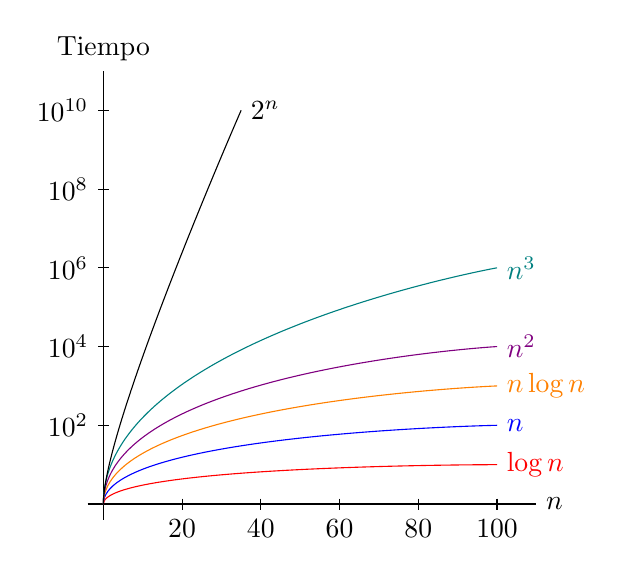
\begin{tikzpicture}

  \draw[] (-0.2,0) -- (5.5,0) node[right] {$n$};
  \draw[] (0,-0.2) -- (0,5.5) node[above] {Tiempo};

  \foreach \x/\xtext in {1/20, 2/40, 3/60, 4/80, 5/100}
  \draw[shift={(\x,0)}] (0pt,2pt) -- (0pt,-2pt) node[below] {$\xtext$};

  \foreach \y/\ytext in {1/10^2, 2/10^4, 3/10^6, 4/10^8, 5/10^{10}}
  \draw[shift={(0,\y)}] (2pt,0pt) -- (-2pt,0pt) node[left] {$\ytext$};

  \draw[red] (0,0)   .. controls +(up:.5cm) and +(left:0cm) .. (5,.5) node [right] {$\log n$};
  \draw[blue] (0,0)   .. controls +(up:.9cm) and +(left:0cm) .. (5,1) node [right] {$n$};
  \draw[orange] (0,0)   .. controls +(up:1.3cm) and +(left:0cm) .. (5,1.5) node [right] {$n \log n$};
  \draw[violet] (0,0)   .. controls +(up:1.7cm) and +(left:0cm) .. (5,2) node [right] {$n^2$};
  \draw[teal] (0,0)   .. controls +(up:2.1cm) and +(left:0cm) .. (5,3) node [right] {$n^3$};
  \draw[] (0,0)   .. controls +(up:1cm) and +(left:0cm) .. (1.75,5) node [right] {$2^n$};

\end{tikzpicture}
\caption{Representación gráfica de las tasas de crecimiento más frecuentes.}%
\end{minipage}%
\end{figure}%
\end{center}%


El resultado queda reflejado en las siguientes tablas:
\begin{table}[H]
\begin{center}
\begin{tabular}{|c|c|c|c|}
\hline
$t(n)$ & $n=100$ & $n=200$ & $n=1000$ \\
\hline
$k_1\ \log n$ & $1$ h. & $1,15$ h. & $1,5$ h. \\
\hline
$k_2 n$ & $1$ h. & $2$ h. & $10$ h. \\
\hline
$k_3\ n \log n$ & $1$ h. & $2,30$ h. & $15$ h. \\
\hline
$k_4 n^2$ & $1$ h. & $4$ h. & $100$ h. \\
\hline
$k_5 n^3$ & $1$ h. & $8$ h. & $1000$ h. \\
\hline
$k_6 2^n$ & $1$ h. & $1,27\ \cdot\ 10^{30}$ h. & $8,45\ \cdot\ 10^{270}$ h. \\
\hline
\end{tabular}
\caption{Efecto de duplicar y multiplicar por diez el tamaño del problema}
\end{center}
\end{table}



\begin{table}[H]
\begin{center}
\begin{tabular}{|c|c|c|c|}
\hline
$t(n)$ & Tiempo=1h. & Tiempo=2h. & Tiempo=10h. \\
\hline
$k_1\ \log n$ & $n=100$  & $n=10.000$ & $n=10^{20}$ \\
\hline
$k_2 n$ & $n=100$  & $n=200$ & $n=1000$ \\
\hline
$k_3\ n \log n$ & $n=100$ & $n=178$ & $n=703$ \\
\hline
$k_4 n^2$ & $n=100$ & $n=141$ & $n=316$ \\
\hline
$k_5 n^3$ & $n=100$ & $n=126$ & $n=215$ \\
\hline
$k_6 2^n$ & $n=100$ & $n=101$ & $n=103$ \\
\hline
\end{tabular}
\caption{Efecto de duplicar y multiplicar por diez el tamaño del problema}
\end{center}
\end{table}

Los que se comportan de un modo más acorde con las expectativas de un usuario no informático son los de complejidad \emph{lineal} y $O(n \log n)$: al duplicar y multiplicar por diez el tamaño del problema aproximadamente se duplica y se multiplica por diez el tiempo empleado, y al duplicar y multiplicar por diez el tiempo disponible, el tamaño que es posible tratar también se duplica y multiplica por diez.\\

El algoritmo de complejidad \emph{logarítmica} tiene un comportamiento excepcionalmente bueno: doblar y multiplicar por diez el tamaño del problema solo aumenta moderadamente el tiempo de ejecución ($15\%$ y $50\%$, respectivamente), mientras que doblar y multiplicar por diez el tiempo disponible permite tratar problemas enormes ($100$ y $10^{18}$ veces mayores que el problema original).\\

Los órdenes $O(n^2)$ y $O(n^3)$ tienen un comportamiento claramente inferior al lineal. Se observa que un incremento del $100\%$ en el tiempo disponible sólo consigue incrementos respectivamente del $41\%$ y del $26\%$ en el tamaño del problema, incluso al multiplicar por 10 el tiempo disponible solo permite resolver problemas 3,16 y 2,15 veces mayores respectivamente. En general podemos decir que dado un algoritmo de orden $O(n^a)$, multiplicar el tiempo disponible (o la velocidad del computador) por un factor $k$ multiplica el tamaño del problema que es posible tratar por un factor $\varphi^k$. Estos cálculos llevan a la conclusión de que no es posible tratar problemas demasiado grandes con algoritmos que presenten estas tasas de crecimiento.\\

No obstante, los algoritmos cuyas tasas de crecimiento están acotadas superiormente por $n^a$ (para cualquier $a$) se dicen, en conjunto, de complejidad polinomial, y los problemas que resuelven se llaman \textbf{tratables}.\\

La situación es muy distinta para los problemas de complejidad exponencial o mayor, que se llaman \textbf{intratables}. Se llaman así los problemas cuyos mejores algoritmos conocidos tiene tiempos en $O(2^n)$. Un algoritmo de tiempo de ejecución exponencial permite tratar problemas muy pequeños, independientemente de la velocidad del ordenador; observando las tablas vemos que multiplicar el tiempo apenas afecta al tamaño del problema que podemos resolver, y multiplicar el tamaño del problema conduce, en este ejemplo, a tiempos de ejecución del orden de varios billones (como mínimo) de veces la edad del universo.\\

Estas consideraciones nos llevan a la conclusión de que es una buena inversión dedicar tiempo a encontrar algoritmos con mejores tasas de crecimiento. Por ejemplo, pasar un algoritmo de $O(n^2)$ a otro de $O(n \log n)$ es una gran mejora, y lo mismo podríamos decir si se encontrara un algoritmo de $O(\log n)$ para problemas que se resolvían en $O(n)$.\\

En sentido contrario, invertir tiempo en ahorrar ésta o aquella variable en un programa, o en mejorar algún caso particular, no cambia generalmente la tasa de crecimiento del algoritmo, sino tan sólo disminuye ligeramente la constante multiplicativa. Además suele oscurecer su comprensión, por tanto no es una inversión rentable e incluso puede llegar a ser contraproducente. \\

\subsection{Indecibilidad}

El propósito de esta sección es proporcionar una introducción informal, basada en el lenguaje de programación C, para mostrar un problema específico que los computadores no pueden resolver. El problema concreto que vamos a examinar tiene por objeto detectar si lo primero que imprime un programa C es \emph{hola, mundo}. Aunque podría imaginarse que la simulación del programa nos permitiría descubrir lo que hace, en realidad tenemos que enfrentarnos con programas que tardan un tiempo inimaginable largo para producir alguna respuesta. Este problema (no saber cuándo ocurre algo, si es que llega ha producirse) es la causa última de nuestra incapacidad para descubrir lo que hace un programa. Sin embargo, es bastante difícil demostrar formalmente que no existe ningún programa capaz de realizar una cierta tarea preestablecida, y es necesario desarrollar algún mecanismo para ello.

\subsubsection{Programas que imprimen ``hola, mundo''}

En el siguiente fragmento de código se presenta el primer programa en C que encuentran los estudiantes que leen el ya clásico libro de Kernighan y Ritchie\footnote{B.W. Kernighan y D.M. Ritchie, \emph{The C Programming Language}, 1978, Prentice-Hall, Englewood Cliffs, NJ.}. Es bastante fácil descubrir que este programa imprime \emph{hola, mundo} y termina. El programa es tan simple que se ha convertido en una práctica habitual introducir los lenguajes de programación cómo se escribe un programa que imprima \emph{hola, mundo} en dichos lenguajes. \\

\begin{Verbatim}[commandchars=\\\{\}]
\PY{c+cp}{\PYZsh{}}\PY{c+cp}{include<stdio.h>}

\PY{k+kt}{int} \PY{n+nf}{main}\PY{p}{(}\PY{p}{)}
\PY{p}{\PYZob{}}
  \PY{n}{printf}\PY{p}{(}\PY{l+s}{"}\PY{l+s}{hola, mundo}\PY{l+s+se}{\PYZbs{}n}\PY{l+s}{"}\PY{p}{)}\PY{p}{;}

  \PY{k}{return} \PY{l+m+mi}{0}\PY{p}{;}
\PY{p}{\PYZcb{}}
\end{Verbatim}


Sin embargo, existen otros programas que también imprimen \emph{hola, mundo} a pesar de que lo que hacen no es ni mucho menos evidente. El siguiente fragmento de código presenta otro programa que quizá imprima \emph{hola, mundo}. Este programa toma una entrada $n$ y busca soluciones enteras positivas de la ecuación $x^n + y^n = z^n$. Si encuentra una solución, imprime \emph{hola, mundo}. Si nunca encuentra enteros $x, y$ y $z$ que satisfagan la ecuación, entonces continúa buscando para siempre, y nunca imprime \emph{hola, mundo}.\\

Para comprender qué hace el programa, digamos primero que $exp$ es una función auxiliar para calcular potencias. El programa principal tiene que buscar las tuplas $(x,y,z)$ en un orden tal que estemos seguros de encontrar, finalmente, todas las tuplas de enteros positivos. Para organizar la búsqueda de forma apropiada, se utiliza una cuarta variable, \emph{total}, cuyo valor inicial es 3, y que, en el bucle while, va incrementándose en una unidad, tomando siempre valores enteros finitos. Dentro del bucle while, \emph{total} se divide en tres números enteros positivos, $x, y,$ y $z$, haciendo primero que $x$ varíe desde 1 hasta \emph{total-2}, y, dentro del bucle for, haciendo que $y$ varíe desde 1 hasta una unidad menos de lo que queda de \emph{total} después de haberle restado el valor actual de $x$. A $z$ se le asigna la cantidad restante, que debe estar entre 1 y \emph{total-2}.\\

\underline{El último teorema de Fermat expresado como un programa hola-mundo}
\begin{Verbatim}[commandchars=\\\{\}]
\PY{c+cp}{\PYZsh{}}\PY{c+cp}{include <stdlib.h>}
\PY{c+cp}{\PYZsh{}}\PY{c+cp}{include <stdio.h>}

\PY{k+kt}{int} \PY{n+nf}{exp}\PY{p}{(}\PY{k+kt}{int} \PY{n}{i}\PY{p}{,} \PY{k+kt}{int} \PY{n}{n}\PY{p}{)}
\PY{c+cm}{/* calcula i a la potencia n */}
\PY{p}{\PYZob{}}
  \PY{k+kt}{int} \PY{n}{ans}\PY{p}{,} \PY{n}{j}\PY{p}{;}
  \PY{n}{ans} \PY{o}{=} \PY{l+m+mi}{1}\PY{p}{;}
  \PY{k}{for} \PY{p}{(}\PY{n}{j}\PY{o}{=}\PY{l+m+mi}{1}\PY{p}{;} \PY{n}{j} \PY{o}{<}\PY{o}{=} \PY{n}{n}\PY{p}{;} \PY{n}{j}\PY{o}{+}\PY{o}{+}\PY{p}{)} \PY{n}{ans} \PY{o}{*}\PY{o}{=} \PY{n}{i}\PY{p}{;}
  \PY{k}{return}\PY{p}{(}\PY{n}{ans}\PY{p}{)}\PY{p}{;}
\PY{p}{\PYZcb{}}

\PY{k+kt}{int} \PY{n+nf}{main}\PY{p}{(}\PY{p}{)}
\PY{p}{\PYZob{}}
  \PY{k+kt}{int} \PY{n}{n}\PY{p}{,} \PY{n}{total}\PY{p}{,} \PY{n}{x}\PY{p}{,} \PY{n}{y}\PY{p}{,} \PY{n}{z}\PY{p}{;}
  \PY{n}{scanf}\PY{p}{(}\PY{l+s}{"}\PY{l+s}{\PYZpc{}d}\PY{l+s}{"}\PY{p}{,}\PY{o}{&}\PY{n}{n}\PY{p}{)}\PY{p}{;}
  \PY{n}{total} \PY{o}{=} \PY{l+m+mi}{3}\PY{p}{;}
  \PY{k}{while}\PY{p}{(}\PY{l+m+mi}{1}\PY{p}{)}\PY{p}{\PYZob{}}
    \PY{k}{for}\PY{p}{(}\PY{n}{x}\PY{o}{=}\PY{l+m+mi}{1}\PY{p}{;} \PY{n}{x} \PY{o}{<}\PY{o}{=} \PY{n}{total} \PY{o}{-} \PY{l+m+mi}{2}\PY{p}{;} \PY{n}{x}\PY{o}{+}\PY{o}{+}\PY{p}{)}
      \PY{k}{for}\PY{p}{(}\PY{n}{y}\PY{o}{=}\PY{l+m+mi}{1}\PY{p}{;} \PY{n}{y} \PY{o}{<}\PY{o}{=} \PY{n}{total} \PY{o}{-}\PY{n}{x} \PY{o}{-}\PY{l+m+mi}{1}\PY{p}{;} \PY{n}{y}\PY{o}{+}\PY{o}{+}\PY{p}{)}
	\PY{p}{\PYZob{}}
	  \PY{n}{z} \PY{o}{=} \PY{n}{total} \PY{o}{-} \PY{n}{x} \PY{o}{-} \PY{n}{y}\PY{p}{;}
	  \PY{k}{if}\PY{p}{(}\PY{n}{exp}\PY{p}{(}\PY{n}{x}\PY{p}{,}\PY{n}{n}\PY{p}{)} \PY{o}{+} \PY{n}{exp}\PY{p}{(}\PY{n}{y}\PY{p}{,}\PY{n}{n}\PY{p}{)} \PY{o}{=}\PY{o}{=} \PY{n}{exp}\PY{p}{(}\PY{n}{z}\PY{p}{,}\PY{n}{n}\PY{p}{)}\PY{p}{)}
	    \PY{n}{printf}\PY{p}{(}\PY{l+s}{"}\PY{l+s}{hola, mundo}\PY{l+s+se}{\PYZbs{}n}\PY{l+s}{"}\PY{p}{)}\PY{p}{;}
	\PY{p}{\PYZcb{}}
    \PY{n}{total}\PY{o}{+}\PY{o}{+}\PY{p}{;}
  \PY{p}{\PYZcb{}}
\PY{p}{\PYZcb{}}
\end{Verbatim}


En el bucle más interno, se comprueba si la tupla $(x,y,z)$ verifica la ecuación $x^n + y^n = z^n$. Si es así, el programa imprime \emph{hola, mundo}, y si no, no imprime nada.\\

Si el valor de $n$ leído por el programa es 2, entonces acabará encontrando combinaciones de enteros tales como $total = 12, x = 3, y = 4$ y $z = 5$, para las cuales $x^n + y^n = z^n$. De modo que, teniendo 2 como entrada, \emph{sí} imprime \emph{hola, mundo}.\\

Sin embargo, para cualquier entero $n > 2$, el programa nunca encontrará una tupla de enteros positivos que satisfaga $x^n + y^n = z^n$ y, por tanto, nunca llegará a imprimir \emph{hola, mundo}. Lo curioso del caso es que hasta hace pocos años no se sabía si este programa imprimiría o no \emph{hola, mundo} para algunos número enteros $n$ grandes. La afirmación de que no lo haría, esto es, de que no existen soluciones enteras para la ecuación $x^n y^n = z^n$ si $n > 2$, fue realizada por Fermat hace 300 años, pero no pudo demostrarse hasta hace bastante poco. Esta proposición recibe a menudo el nombre de ``último teorema de Fermat''.\\

Definamos así el \emph{problema hola-mundo}: determinar si un programa C dado, con una cierta entrada, imprime en primer lugar los 11 caracteres de \emph{hola, mundo}. \\

Parece probable que, si a los matemáticos les llevó 300 años resolver una pregunta acerca de un único programa de 22 líneas, entonces debe ser realmente difícil decidir el problema general de si un programa dado, con una cierta entrada, imprime o no \emph{hola, mundo}. De hecho, cualquiera de los problemas que los matemáticos todavía no han podido resolver puede plantearse como una pregunta de la forma ``¿este programa, con esta entrada, imprime \emph{hola, mundo}?''. Así que sería realmente extraordinario que fuéramos capaces de escribir un programa que pudiera examinar cualquier programa $P$ y cualquier entrada $I$ para $P$ y decir si $P$, al ejecutarlo con $I$ como entrada, imprimirá \emph{hola, mundo}. Dicha demostración de que tales programas no existen queda fuera de este contexto de estudio.\\

\subsubsection{Por qué tienen que existir problemas indecidibles}

Aunque es delicado demostrar que un problema específico, como el ``problema hola-mundo'' que acabamos de examinar, es indecidible, es bastante sencillo comprender por qué casi todos los problemas han de ser indecidibles para los sistemas relacionados con la programación. Recordemos que un ``problema'' en realidad se ha definido como una pregunta acerca de si cierta cadena forma parte de un lenguaje. El número de lenguajes diferentes con cualquier alfabeto de más de un símbolo no es numerable; esto es, no hay forma de asignar números enteros a los lenguajes de manera que cada lenguaje tenga asignado un número entero y cada número entero corresponda a un lenguaje. \\

Por otra parte, los programas \emph{son} numerables, por se cadenas finitas construidas con un alfabeto finito (normalmente, un subconjunto del alfabeto ASCII). Es decir, es posible ordenarlos de acuerdo con su longitud, por orden alfabético. Por tanto, podemos hablar del primer programa, el segundo programa y, en general, del $i$-ésimo para cualquier entero $i$.\\

Como consecuencia, sabemos que existen infinitos programas menos que problemas. Si eligiéramos un lenguaje al azar, casi seguro que correspondería a un problema indecidible. La única razón por la que la mayoría de los problemas \emph{parece} que son decidibles es porque los problemas elegidos al azar rara vez tienen interés. Más bien, tendemos a considerar problemas bastante sencillos y bien estructurados, y estos problemas que nos interesan, y que pueden enunciarse clara y brevemente, es posible encontrar muchos indecidibles; el problema hola-mundo es uno de ellos.\\

\vspace{-.25in}{
\subsection{La máquina de Turing}

La teoría de los problemas indecidibles no solo tiene por objeto establecer la existencia de dichos problemas (una idea emocionante por sí sola desde el punto de vista intelectual), sino proporcionar a los programadores una guía sobre lo que se puede llevar a cabo o no llevar a cabo mediante la programación. Para los programadores y diseñadores de sistemas, estos problemas, llamados ``problemas intratables'', tienden a presentar más dificultades que los problemas indecidibles. La razón para ello es que, mientras que suele ser obvio que los problemas indecidibles efectivamente lo son y, en la práctica, raramente se intentan resolver, los problemas intratables aparecen continuamente. Además, a menudo dan lugar a pequeñas modificaciones de los requisitos o a soluciones heurísticas. Por tanto, los diseñadores tienen que enfrentarse frecuentemente al hecho de tener que decidir si un problema es o no intratable, y qué hacer si lo es.\\}

Hacen falta herramientas que nos permitan determinar la indecidibilidad  o intratabilidad de los problemas de cada día. La tecnología que se introdujo en la sección anterior es útil para las cuestiones que se plantean acerca de los programas, pero no se puede trasladar fácilmente a problemas de otros dominios no relacionados. Por ejemplo, podríamos tener grandes dificultades para reducir el problema hola-mundo a la cuestión de si una gramática es ambigua.\\

En consecuencia, necesitamos reconstruir la teoría de la indecibilidad, no ya basándonos en programas escritos en C o cualquier otro lenguaje de programación, sino en un modelo muy simple de computador, denominado máquina de Turing. Este dispositivo es esencialmente un autómata finito que dispone de una cinta de longitud infinita sobre la que puede leer y escribir datos. Una de las ventajas de la máquina de Turing sobre los programas, como mecanismo de representación de lo que se puede computar, es que la máquina de Turing es suficientemente sencilla como para que su configuración pueda representarse con precisión, utilizando una notación simple del estilo de las configuraciones de los autómatas a pila. En cambio, aunque los programas en C tiene un estado, que depende de todas las variables, sea cual sea la secuencia de llamadas a las función que se realice, la notación que hay que utilizar para describirlo es demasiado compleja como para permitirnos realizar demostraciones formales comprensibles.\\

Utilizando la notación de la máquina de Turing, probaremos que son indecidibles ciertos problemas que, aparentemente, no tienen relación con la programación.\\

\subsubsection{El intento de decidir todas las cuestiones matemáticas}

A finales del siglo XIX, el matemático D. Hilbert se preguntó si era posible encontrar un algoritmo para determinar la verdad o falsedad de cualquier posición matemática. En particular, se preguntaba si existiría un modo de determinar si cualquier fórmula del cálculo de predicados de primer orden, aplicada a enteros, es verdadera. Dado que el cálculo de predicados de primer orden sobre los enteros es suficientemente potente como para expresar frases como ``esta gramática es ambigua'', o ``este programa imprime \emph{hola, mundo}'', si Hilbert hubiera tenido éxito, existirían algoritmos para dichos problemas, que ahora sabemos que no existen.\\

Sin embargo, en 1931, K. Gödel publicó su famoso teorema de la incompletitud. Gödel construyó una fórmula del cálculo de predicados aplicado a enteros que afirmaba que la propia fórmula no podía ser probada, ni refutada, dentro del cálculo de predicados. \\

El cálculo de predicados no era la única idea que tenían los matemáticos para ``cualquier computación posible''. De hecho, el cálculo de predicados, al ser declarativo más que computacional, entraba en competencia con una variedad de notaciones, incluidas las ``funciones recursivas parciales'' (una notación parecida a un lenguaje de programación) y otras notaciones similares. En 1936, A.M. Turing propuso la máquina que lleva su nombre como modelo de ``cualquier computación posible''. Este modelo se parece más a un computador que a un programa, aunque los verdaderos computadores electrónicos, o incluso los electromecánicos, tardaron varios años en llegar. \\

Lo curioso del caso es que todas las propuestas serias sobre modelos de computación tienen el mismo potencial, es decir, computan exactamente las mismas funciones y reconocen los mismos lenguajes. La suposición no demostrada de que cualquier forma general de computación nos permitirá calcular únicamente las funciones recursivas parciales (o, lo que es lo mismo, lo que las máquinas de Turing o los computadores modernos pueden calcular) se conoce como \emph{hipótesis de Church}(en honor al lógico A. Church) o \emph{tesis de Church-Turing}.\\

\subsection{Notación para la máquina de Turing}

Podemos imaginarnos una máquina de Turing como la que se ha presentado en la siguiente figura. La máquina consta de una \emph{unidad de control}, que puede estar en cualquier estado tomado de un conjunto finito. Hay una cinta dividida en cuadrados o \emph{casillas}, y cada casilla puede contener un símbolo, tomado de otro conjunto finito.\\

\figuratikz{1}{Una máquina de Turing.}
{
  \tikzstyle{texto}=[]
  
  \draw (1,1) +(-.5,-.5) rectangle ++(.5,.5);
  \draw (1,1) node{$\cdots$};

  \draw (2,1) +(-.5,-.5) rectangle ++(.5,.5);
  \draw (2,1) node{$B$};

  \draw (3,1) +(-.5,-.5) rectangle ++(.5,.5);
  \draw (3,1) node{$B$};

  \draw (4,1) +(-.5,-.5) rectangle ++(.5,.5);
  \draw (4,1) node{$X_1$};

  \draw (5,1) +(-.5,-.5) rectangle ++(.5,.5);
  \draw (5,1) node{$X_2$};

  \draw (6,1) +(-.5,-.5) rectangle ++(2.5,.5);

  \draw (9,1) +(-.5,-.5) rectangle ++(.5,.5);
  \draw (9,1) node (d1) {$X_i$};

  \draw (10,1) +(-.5,-.5) rectangle ++(1.5,.5);

  \draw (12,1) +(-.5,-.5) rectangle ++(.5,.5);
  \draw (12,1) node{$X_n$};

  \draw (13,1) +(-.5,-.5) rectangle ++(.5,.5);
  \draw (13,1) node{$B$};

  \draw (14,1) +(-.5,-.5) rectangle ++(.5,.5);
  \draw (14,1) node{$B$};

  \draw (15,1) +(-.5,-.5) rectangle ++(.5,.5);
  \draw (15,1) node{$\cdots$};

  \draw[ultra thick,white] (16,1) +(0,-.5) rectangle ++(-.5,.5);
  \draw[ultra thick,white] (0,1) +(0,-.5) rectangle ++(.5,.5);

  \draw (8,3) +(0,0) rectangle ++(2,2);

  \node [texto] (t1) [above of=d1,yshift=2cm] {de};
  \node [texto] (t2) [above of=t1,yshift=-.5cm] {Unidad};
  \node [texto] (t3) [below of=t1,yshift=.5cm] {Control};

  \draw[post] (8.75,3)   .. controls +(50:-2cm) and +(-100:-1cm) .. (9,1.5);

}

Inicialmente, se sitúa en la cinta de \emph{entrada}, que es una cadena de símbolos de longitud finita, elegidos del \emph{alfabeto de entrada}. El resto de las casillas de la cinta, que se extiende infinitamente hacia la derecha y hacia la izquierda, contiene, inicialmente,  un símbolo denominado \emph{espacio en blanco}. El espacio en blanco es un \emph{símbolo de cinta}, pero no un símbolo de entrada, y puede haber también otros símbolos de cinta además de los símbolos de entrada y del espacio en blanco.\\

Existe una \emph{cabeza} de la cinta que siempre está situada sobre una de las casillas de la cinta. Se dice que la máquina de Turing está \emph{señalando} dicha casilla. Al principio, la cabeza de la cinta se encuentra en la casilla de la entrada situada más a la izquierda.\\

Un \emph{movimiento} de la máquina de Turing es una función del estado de la unidad de control y del símbolo de la cinta al que señala la cabeza. En un movimiento, la máquina de Turing:
\begin{enumerate}
\item Cambiará de estado. Opcionalmente, el siguiente estado puede ser el mismo que el actual.
\item Escribirá un símbolo de cinta en la casilla señalada por la cabeza. Este símbolo de cinta sustituye al símbolo que estuviera anteriormente en la casilla.
\item Moverá la cabeza de la cinta hacia la izquierda o hacia la derecha. En nuestro formalismo, se exige que haya un movimiento, y no se permite que la cabeza permanezca en el mismo lugar. Esta limitación no restringe lo que una máquina de Turing puede computar, dado que cualquier secuencia de movimientos con la cabeza estacionaria podría condensarse, junto con el movimiento siguiente de la cabeza, en un único cambio de estado, un nuevo símbolo de cinta y un movimiento hacia la izquierda o hacia la derecha.
\end{enumerate}

La notación formal que se suele emplear para una máquina de Turing (MT) es similar a la utilizada para los autómatas finitos o para los autómatas a pila. Una MT se describe mediante la séptupla

\[ M = (Q, \Sigma, \Gamma, \delta, q_0, B, F) \]

cuyas componentes tienen el siguiente significado:\\
\begin{description}
\item[$Q$]: El conjunto finito de \emph{estados} de la unidad de control.
\item[$\Sigma$]: El conjunto finito de \emph{símbolos de entrada}.
\item[$\Gamma$]: El conjunto completo de \emph{símbolos de cinta}; $\Sigma$ siempre es un subconjunto de $\Gamma$.
\item[$\delta$]: \quad La \emph{función de transición}. Los argumentos de $\delta(q,X)$ son un estado $q$ y un símbolo de cinta $X$. El valor de $\delta(q,X)$, si está definido, es una tupla $(p,Y,S)$, donde:
  \begin{enumerate}
  \item $p$ es el estado siguiente de $Q$.
  \item $Y$ es el símbolo de $\Gamma$, que se escribe en la casilla señalada por la cabeza de la cinta y que se sustituye al símbolo que se encontraba en dicha casilla, sea cual fuere.
  \item $S$ es un \emph{sentido}, $I$ o $D$ (``izquierda'' o ``derecha'', respectivamente), que nos indica el sentido en el que se mueve la cabeza.
  \end{enumerate}
\item[$q_o$]: El estado \emph{inicial} (uno de los elementos de $Q$) en el cual se encuentra inicialmente la unidad de control.
\item[$B$]: El símbolo de \emph{espacio en blanco}. Este símbolo forma parte de $\Gamma$ pero no de $\Sigma$; es decir, no es un símbolo de entrada. El espacio en blanco aparece inicialmente en todas las casillas de la cinta, excepto en aquéllas que contienen los símbolos de la entrada.
\item[$F$]: El conjunto de estados \emph{finales} o de aceptación, que constituye un subconjunto de $Q$.
\end{description}

\subsection{Intratabilidad}

El diccionario define \emph{intratable} como "difícil de tratar o de trabajar". Esto significa que un problema en informática es intratable si un ordenador tiene dificultades para resolverlo. Esta definición es demasiado vaga para ser de mucha utilidad para nosotros. Para hacer más concreta la idea, definiremos de manera informal el concepto de algoritmo de tiempo polinómico:\\
\begin{fondo}
Un algoritmo de tiempo polinomial es aquel algoritmo cuya complejidad asintótica para el peor caso es acotado superiormente por una función polinómica de su tamaño de entrada. Es decir, si $n$ es el tamaño de la entrada, existirá un polinomio $p(n)$ tal que
\[ W(n) \in O(p(n)) \].
siendo W(n) la complejidad en el peor caso del algoritmo.
\end{fondo}

En informática, un problema se llama intratable si no es posible resolverlo con un algoritmo de tiempo polinómico. Destacamos que la intratabilidad es una propiedad del problema: esto no es una propiedad de cualquier algoritmo para este problema. Para que un problema sea intratable, no debe de haber ningún algoritmo de tiempo polinómico capaz de resolverlo. La obtención de un tiempo no polinómico para un problema no significa que este sea intratable.\\

En las secciones anteriores hemos visto que los algoritmos de tiempo polinomial suelen ser mucho mejor que los algoritmos que no lo son. Podemos crear ejemplo extremos en los que un algoritmo de tiempo no polinómico es mejor que un algoritmo de tiempo polinómico para tamaños de entrada prácticos. Por ejemplo, si $n = 1.000.000$,\\
\[ 2^{0.00001n} = 1024\ \mbox{mientras}\ n^{10} = 10^{60} \]

Además, muchos algoritmos donde sus complejidades en el peor caso no son polinómicas tienen eficientes tiempos de funcionamiento en muchos casos reales. Este es el caso de muchas técnicas de backtracking y de búsqueda en árboles. Por lo tanto, nuestra definición de intratable sólo es una buena indicación de la dificultad real. En cualquier caso, un problema al que se le ha encontrado un algoritmo de tiempo polinómico podría ser más difícil de manejar, por lo que a los tamaños de ejemplares de entrada prácticos, que para el caso en el que no hayamos podido encontrar tal algoritmo. \\

Hay tres categorías generales de los problemas en cuanto a dificultad se refiere:
\begin{enumerate}
\item Problemas para los cuales se ha encontrado un algoritmo de tiempo polinómico.
\item Problemas que se han demostrado que son intratables.
\item Problemas en los que no se ha demostrado que no sea intratable, pero para los que tampoco se ha encontrado un algoritmo de tiempo polinómico.
\end{enumerate}

Además, es un fenómeno sorprendente que la mayoría de los problemas en informática parecen encuadrarse en las categoría 1ª y 3ª.\\

\subsubsection{Tres categorías de problemas}

A continuación se discuten las tres categorías en las que los problemas se pueden agrupar en cuanto a dificultad se refiere.\\

$\bullet$ \textbf{Problemas para los cuales se ha encontrado un algoritmo de tiempo polinómico.}\\

Cualquier problema en el que hayamos encontrado un algoritmo de tiempo polinómico se sitúa en esta primera categoría. Hemos encontrado algoritmos de ordenación del orden de $O(n \lg n)$, un algoritmo de búsqueda en un vector ordenado del orden de $O(\lg n)$, un algoritmo para la multiplicación de matrices del orden de $O(n^{2.38})$, etc. Dado que $n$ es una medida de la cantidad de datos de entrada para dichos algoritmos, todos ellos serán pues de tiempo polinómico. Hay otros problemas para los cuales hemos desarrollado algoritmos de tiempo polinómico, pero existen algoritmos de fuerza bruta para los cuales resulta obvio que no sean de tiempo polinómico, incluyendo los problemas de caminos más cortos, el problema de la búsqueda binaria en un árbol, y el problema del árbol de expansión mínimo.\\

$\bullet$ \textbf{Problemas que se han demostrado que son intratables.}\\

Hay dos tipos de problemas en esta categoría. El primer tipo son los problemas que requieren una cantidad no polinómica de resultados. Recordemos de la sección 3.2 el problema de la determinación de todos los caminos o circuitos de Hamilton. Si había una arista desde cada vértice hasta todos los demás vértices, entonces podrían existir $(n - 1)!$ circuitos. Para resolver el problema, un algoritmo podría tener una salida para todos los caminos, lo que significaría que nuestro caso no es razonable. El problema de los caminos o circuitos hamiltonianos que requiere de un solo camino claro no es un problema de este tipo. Aunque es importante reconocer este tipo de intratabilidad, problemas como estos normalmente no presentan dificultad alguna. Por lo general es fácil reconocer que se requiera una cantidad no polinómica de resultados, y una vez que los reconocemos, nos damos cuenta de que simplemente estamos pidiendo más información de lo que teníamos posibilidad de uso. Es decir, el problema no es del todo realista.\\

El segundo tipo de estos problemas se presenta cuando nuestras necesidades son razonables (es decir, cuando no estamos pidiendo una cantidad no polinómica de resultados) y podemos demostrar que el problema no puede resolverse en tiempo polinomial. Por extraño que parezca, hemos encontrado varios problemas de este tipo. Los primeros fueron \emph{problemas indecidibles}. Estos problemas se llaman "indecidibles", ya que se puede probar que los algoritmos que los resuelven no pueden existir. El más conocido de ellos es el problema de la parada. En este problema se toma como entrada cualquier algoritmo y cualquier entrada de dicho algoritmo, y se comprueba si se detiene o no la ejecución de dicho algoritmo aplicando la entrada de datos pertinente. En 1936, Alan Turing demostró que este problema es indecidible. En 1953, A. Grzegorczyk desarrolló un problema decidible que fue intratable. Sin embargo, estos problemas fueron "artificialmente" construidos para tener ciertas propiedades. En la década de 1970, algunos de los problemas naturales de decisión decidible demostraron ser intratables. La salida de un problema de decisión es un simple "sí" o "no" como respuesta. Por lo tanto, la cantidad de resultados posibles es razonable. Uno de los más conocidos de estos problemas es el de la aritmética de Presburger, que fue demostrado como intratable por Fischer y Rabin en 1974. Este problema, junto con la prueba de dificultad, se puede encontrar Hopcroft y Ullman (1979).\\

Todos los problemas que hasta la fecha se hayan demostrado como intratables también han sido demostrado que no pertenecen al conjunto NP. Sin embargo, la mayoría de los problemas que aparecen intratables han resultado pertenecer al conjunto NP.

$\bullet$ \textbf{Problemas en los que no se ha demostrado que no sea intratable, pero para los que tampoco se ha encontrado un algoritmo de tiempo polinómico.}

Esta categoría incluye cualquier problema para el que no se ha encontrado un algoritmo de tiempo polinómico, pero todavía nadie ha demostrado que este tipo de algoritmos no sean posibles. Como ya hemos comentado, hay muchos de esos problemas. Por ejemplo, si tenemos en cuenta que los problemas deban tener una solución, el problema de la mochila 0-1, el problema del viajero, el problema de la suma de subconjuntos, el problema de m-coloreado para un $m \geq 3$, el problema de los caminos hamiltonianos, y el problema de la inferencia abductiva en una red bayesiana todos deben entran en esta categoría. Hemos encontrado algoritmos de ramificación, algoritmos de backtracking, y otros algoritmos para estos problemas que son más eficientes en muchos casos grandes. Es decir, hay un polinomio en $n$ que limita el número de veces que la operación básica se ejecuta cuando los casos que se toman de un subconjunto restringido. Sin embargo, no existe tal polinomio para el conjunto de todos los casos. Para demostrar esto, sólo tenemos que encontrar una secuencia infinita de casos para los que un no polinomio en $n$ limite el número de veces que se realiza la operación básica.\\

\section{NP-completitud}\label{sec:NP-section}

En la vida real existen muchos problemas prácticos para los cuales no se conoce ningún algoritmo eficiente, pero cuya dificultad intrínseca no ha conseguido demostrar nadie. Entre estos se cuentan problemas tan conocidos como el del viajante de comercio, el coloreado óptimo de grafos, el problema de la mochila, los ciclos hamiltonianos, la programación entera, la búsqueda del camino simple más largo de un grafo, y la satisfacción de una fórmula booleana. ¿Hay que culpar a la algorítmica o a la complejidad? Quizá existan realmente algoritmos eficientes para estos problemas. Después de todo, las ciencias de la computación son relativamente recientes: es claro que quedan por descubrir nuevas técnicas algorítmicas.\\

En esta sección presentamos un resultado notable: un algoritmo eficiente para resolver cualquier de los problemas enumerados en el párrafo anterior proporcionaría automáticamente algoritmos eficientes para todos ellos. No sabemos si estos problemas son fáciles o difíciles de resolver, pero ciertamente sabemos que todos ellos son de complejidad parecida. La importancia práctica de estos problemas ha asegurado que cada uno de ellos por separado haya sido objeto de esfuerzos sostenidos para hallar un método de solución eficiente. Por esta razón, la creencia de que no existen tales algoritmos se encuentra ampliamente difundida. Si se tiene que resolver un problema, y uno puede demostrar que es computacionalmente equivalente a uno de los mencionados anteriormente, es posible tomar esto como evidencia convincente - pero no como demostración - de que el problema es difícil en el caso peor. \\

En el núcleo de esta teoría yace la idea de que puede haber problemas que sean realmente difíciles de resolver, pero para los cuales se puede verificar eficientemente la validez de cualquier supuesta solución. Consideremos el \emph{problema del ciclo hamiltoniano} como ejemplo. Dado un grafo no dirigido $G = (V,A)$, el problema consiste en hallar un camino que comience en algún nodo, visite cada nodo exactamente una vez, y vuelva al nodo de partida. Decimos que un grafo es hamiltoniano si existe uno de estos ciclos. Se cree que el problema es difícil. Sin embargo, es obviamente fácil verificar si una cierta sucesión de nodos define un ciclo hamiltoniano. Otro ejemplo es la factorización. Dado un número compuesto, puede ser difícil hallar un divisor no trivial, pero es sencillo verificar la validez de cualquier supuesto divisor. Quizá parezca evidente que para muchos problemas resulta realmente más sencillo verificar la validez de una supuesta condición que encontrar una solución partiendo de cero. El mayor desconcierto de la moderna teoría de la complejidad computacional es que no sabemos demostrar esto.\\

\section{Las clases P y NP}

Antes de seguir adelante, nos servirá de ayuda definir lo que entendemos por un algoritmo eficiente. ¿Significa esto que requiere un tiempo que está en $O(n \log n)$? ¿En $O(n^2)$ ¿En $O(n^{2,81})$? Todo depende del problema que hay que resolver. Un algoritmo de ordenación que requiere un tiempo en $O(n^2)$ es ineficiente, mientras que un algoritmo de multiplicación matricial que requiera un tiempo en $O(n^2 \log n)$ sería un descubrimiento asombroso. Por tanto, podemos sentir la tentación de decir que un algoritmo posible para resolver nuestro problema. Sin embargo, esta definición sería imprecisa y resultaría difícil trabajar con ella, y en algunos casos ``el mejor algoritmo posible'' ni siquiera existe. Además, existen problemas para los cuales hasta el mejor algoritmo posible requiere una cantidad de tiempo exorbitante, incluso para casos pequeños. ¿No sería razonable admitir que estos problemas son inherentemente intratables, en lugar de afirmar que unos algoritmos inteligentes son eficientes aunque resulten demasiado lentos para utilizarlos en la práctica?\\

Para nuestros propósitos actuales, responderemos a esta pregunta estipulando que un algoritmo es \emph{eficiente} si existe un polinomio $p(n)$ tal que el algoritmo puede resolver cualquier caso de tamaño $n$ en un tiempo que está en $O(p(n))$. Diremos que estos algoritmos son de \emph{tiempo polinómico}. Los algoritmos de tiempo exponencial se vuelven rápidamente inútiles en la práctica, mientras que en general un algoritmo de tiempo polinómico nos permite resolver casos mucho mayores.\\

Esta noción de eficiencia no debe de tomarse ligeramente. Dados dos algoritmos que requieran un tiempo en $O(n^{\lg \lg n})$ y en $O(n^{10})$ respectivamente, el primero es ineficiente según nuestra definición porque no es de tiempo polinómico. Sin embargo, vencerá al algoritmo de tiempo polinómico en todos los casos de tamaño menor que $10^{300}$, suponiendo que las constantes ocultas sean parecidas. De hecho, no es razonable afirmar que un algoritmo que requiera un tiempo en $O(n^{10})$ sea eficiente en la práctica. Sin embargo, decretar que es eficiente mientras que $O(n^4)$ no lo es, por ejemplo, sería excesivamente arbitrario. Además, incluso un algoritmo de tiempo lineal puede no ser utilizable en la práctica si la constante multiplicativa oculta es demasiado grande, mientras que un algoritmo que requiera un tiempo exponencial en el caso peor puede resultar sumamente rápido en la mayoría de los casos. Sin embargo, existen ventajas técnicas significativas cuando se considera la clase de todos los algoritmos de tiempo polinómico. En particular, todos los modelos razonables de computación determinista con un solo procesador se pueden simular entre sí con una pérdida de velocidad que es, como mucho, polinómica. Por tanto, la noción de computabilidad en tiempo polinómica es robusta: no depende del modelo que se prefiera, a no ser que se utilicen modelos posiblemente más potentes como las computadoras probabilistas o cuánticas. Además, el hecho de que las sumas, productos y composiciones de polinomios sean a su vez polinomios resultará útil.\\

\begin{fondo}
P es la clase de problemas de decisión que se pueden resolver mediante un algoritmo de tiempo polinómico.
\end{fondo}

La teoría de la NP-completitud estudia la noción de propiedades \emph{verificables} polinómicamente. Intuitivamente, un problema de decisión $X$ es verificable eficientemente si un ser omnisciente pudiera producir una evidencia convincente de que $x \in X$ sin más contacto con el mencionado ser. Sin embargo, si $x \in X$, no deberíamos quedar falsamente convencidos de que $x \in X$ independientemente de lo que nos diga el ser. Considere como ejemplo el problema consistente en decidir si un grafo es hamiltoniano. Aun cuando se cree que este problema es difícil, es verificable eficientemente: si el ser nos muestra un ciclo hamiltoniano, es sencillo verificar si es o no correcto. Por otra parte, nada de lo que nos muestre el ser - con la posible excepción de una metralleta - podrá convencernos de que el grafo es hamiltoniano si no lo es realmente.\\

Considere un problema de decisión $X$. Sea $Q$ un conjunto, arbitrario por el momento, al que llamaremos \emph{espacio de prueba} para $X$. Un \emph{sistema de prueba} para $X$ es un conjunto de $F$ parejas $\langle x, q \rangle$. Para todo $x \in X$, tiene que existir al menos un $q \in Q$ tal que $\langle x, y \rangle \in F$; por otra parte, cuando $x \notin X$, no debe de existir ninguno de estos $q$. Por tanto, basta que el ser nos muestre algún $q \in Q$ tal que $\langle x, q \rangle \in F$ para convencernos de que $x \in X$. Al ver este $q$ quedaremos convencidos de que $x$ es un caso-si (es decidible), dado que si $x$ fuera un caso-no (no decidible), no existiría ningún $q$ para los casos-si porque siempre existen por definición. Formalmente, $F$ es un subconjunto de $X \times Q$ tal que
\[ (\forall x \in X)(\exists q \in Q)[\langle x, q \rangle \in F] \]
Todo $q$ tal que $\langle x, q \rangle \in F$ se denomina \emph{prueba} o bien \emph{certificado} de que $x \in X$. No hemos especificado explícitamente en la definición formal anterior que
\[ (\forall x \notin X)(\forall q \in Q)[\langle x, q \rangle \notin F] \]
porque está implícito en el requisito de que $F$ tiene que ser un subconjunto de $X \times Q$.\\
Por ejemplo, si $X$ es el conjunto de todos los grafos hamiltonianos, podemos tomar como $Q$ el conjunto de sucesiones de nodos del grafo, y definimos $\langle G, s \rangle \in F$ si y solo si la sucesión de nodos $s$ especifica un ciclo hamiltoniano en el grafo $G$.\\
Otro ejemplo más: si $X$ es el conjunto de todos los números compuestos, podemos tomar $Q = \mathbb{N}$ como espacio de pruebas y
\[ F = \Bigl\{\langle n, q \rangle \Bigl| 1 < q < n\ \mbox{y}\ q\ \mbox{divide a}\ n \Bigl\} \]
como sistema el de pruebas. Este sistema de prueba no es único. Otra posibilidad podría ser
\[ F' = \Bigl\{\langle n, q \rangle \Bigl| 1 < q < n\ \mbox{y mcd}(q,n) \notin 1 \Bigl\} \]
La clase NP corresponde a los problemas de decisión que tienen un sistema de prueba \emph{eficiente}, lo cual significa que todo caso-si (es decidible) debe poseer al menos un certificado \emph{sucinto}, cuya validez pueda ser verificada rápidamente.\\

\begin{fondo}
\label{eq:def} 
NP es la clase de problemas de decisión que admiten un sistema de pruebas $F \subseteq X \times Q$ tal que existe un polinomio $p(n)$ y un algoritmo de tiempo polinómico $A$ tal que
\begin{itemize}
\item Para todo $x \in X$ existe un $q \in Q$ tal que $\langle x, q \rangle \in F$ y además el tamaño de $q$ es como máximo $p(n)$, donde $n$ es el tamaño de $x$.
\item Para todos los pares $\langle x, q \rangle$, el algoritmo $A$ puede verificar si $\langle x, q \rangle$ pertenece o no a $F$. En otras palabras, $F \in P$.
\end{itemize}
\end{fondo}

Los dos ejemplos anteriores encajan en esta definición. Un ciclo hamiltoniano en un grafo, si existe, requiere menos espacio para describirlo que el grafo, y se puede verificar en un tiempo lineal si una sucesión de nodos forma un ciclo hamiltoniano. De forma similar, todo factor no trivial de un número compuesto es menor que ese número, y basta una sola división para verificar su validez. Por tanto, estos dos problemas están en NP.\\

Antes de seguir adelante, hay que hacer una advertencia seria: quizá se sienta tentado a pensar que las letras NP quieren decir ``no polinómico''. ¡No es así! Esto sería una tontería porque (1) todo problema que se pueda resolver en un tiempo polinómico está automáticamente en NP (siguiente teorema) y (2) no conocemos la forma de demostrar la existencia de algún problema en NP que no se pueda resolver en tiempo polinómico, aunque conjeturamos que existen. De hecho, NP quiere decir \textbf{tiempo polinómico no determinista}.\\

Otro posible asunto problemático es que la definición de NP es asimétrica: requerimos la existencia de certificados sucintos para todos los casos-si (es decidible), pero no existe ese requisito para los casos-no (no decidible). Aun cuando el conjunto de todos los grafos hamiltonianos está claramente en NP, no existe tal evidencia para el conjunto de todos los grafos \emph{no} hamiltonianos. De hecho, ¿qué clase de evidencia sucinta podría convencernos eficientemente de que un grafo \emph{no} es hamiltoniano cuando lo es? Se conjetura que en general no puede existir tal evidencia, y por tanto que el conjunto de todos los grafos no hamiltonianos no está en NP.

\begin{fondo}
Teorema: $P \subseteq NP$
\end{fondo}

\underline{Demostración}\\
Intuitivamente, este resultado se debe a que no necesitamos ayuda de un ser omnisciente cuando podemos manejar por nosotros mismos el problema de decisión. Formalmente, consideremos un problema de decisión arbitrario $X \in P$. Sea $Q = \{0\}$ un espacio de pruebas trivial. Definimos
\[ F = \Bigl\{ \langle x, 0 \rangle \Bigl| x \in X \Bigl\} \]
Claramente, todo caso-si admite un ``certificado'' sucinto, a saber, 0, y los caos-no carecen por completo de certificados. Además, basta verificar que $x \in X$ para establecer que $\langle x, q \rangle \in F$. Esto se puede hacer en tiempo polinómico precisamente porque hemos supuesto que $X \in P$.\\
La cuestión fundamental que sigue abierta es si la inclusión de conjuntos del Teorema anterior es o no propia. ¿Es posible que P = NP? Si tal cosa ocurriese, toda propiedad que pudiera verificarse en tiempo polinómico dado un certificado,  podría decidirse también en tiempo polinómico partiendo de cero. Aunque esto parece imposible, nadie ha sido capaz de zanjar esta cuestión. En el resto de la sección analizaremos las consecuencias de la \emph{conjetura}
\[ P \neq NP \]
Para esto, necesitamos una noción de reducción que nos permita comparar la dificultad intrínseca de los problemas NP y descubrir que hay problemas en NP que son tan difíciles como cualquier otro problema de NP. Tales problemas, que se denominan \emph{NP-completos}, se pueden resolver en tiempo polinómico si y solo si todos los demás problemas de NP se pueden resolver también en tiempo polinómico, lo cual equivale a decir que $P = NP$. Por tanto, con la conjetura $P \neq NP$, sabemos que los problemas NP-completos no se pueden resolver en tiempo polinómico.\\

\subsection{Reducciones polinómicas}

\begin{fondo}
Sean \textbf{A} y \textbf{B} dos problemas. Diremos que \textbf{A} es polinómicamente Turing reducible a \textbf{B} si existe un algoritmo para resolver \textbf{A} en un tiempo que sería polinómico si pudiéramos resolver casos arbitrarios del problema \textbf{B} con coste unitario. Esto se denota \textbf{A} $\bf{\leq} _{T}^p$ \textbf{B}. Cuando \textbf{A} $\bf{\leq} _{T}^p$ \textbf{B} y \textbf{B} $\bf{\leq} _{T}^p$ \textbf{A} son ciertos ambos, decimos que \textbf{A} y \textbf{B} son polinómicamente Turing equivalentes y escribimos \textbf{B} $\bf{\equiv} _{T}^p$ \textbf{A}.
\end{fondo}

En otras palabras, el algoritmo para resolver el problema \textbf{A} puede utilizar como le plazca un algoritmo imaginario que puede resolver el problema \textbf{B} con coste unitario. Este algoritmo imaginario se denomina a veces \emph{oráculo}. Como en el caso lineal, la demostración por reducción suele adoptar la forma de un algoritmo explícito para resolver un problema mediante llamadas a un algoritmo arbitrario para el otro problema. Una vez más, esto se podría utilizar para enseñar a alguien que sepa resolver uno de los problemas mediante llamadas a un algoritmo arbitrario para el otro problema. Una vez más, esto se podría utilizar para enseñar a alguien que sepa resolver uno de los problemas a resolver el otro. Y también de nuevo, las reducciones polinómicas son transitivas: si \textbf{A} $\bf{\leq} _{T}^p$ \textbf{B} y \textbf{B} $\bf{\leq} _{T}^p$ \textbf{C}, entonces \textbf{A} $\bf{\leq} _{T}^p$ \textbf{C}. A diferencia de las reducciones lineales, sin embargo, permitimos que el primer algoritmo requiera una cantidad polinómica de tiempo, contando las llamadas al segundo algoritmo como de coste unitario, y llamar al segundo algoritmo un número polinómico de veces para casos arbitrarios de tamaño polinómico respecto al tamaño del ejemplar original.\\

Consideremos dos problemas \textbf{A} y \textbf{B} tales que \textbf{A} $\bf{\leq}_{T}^p$ \textbf{B}. Sea $p(n)$ un polinomio tal que el algoritmo de reducción para el problema \textbf{A} nunca requiere la resolución de más de $p(n)$ casos del problema \textbf{B} cuando se resuelve un caso de tamaño $n$, y tal que ninguno de esos casos es de tamaño mayor que $p(n)$. Este polinomio tiene que existir, porque en caso contrario el algoritmo de reducción requeriría un tiempo mayor que el polinómico, incluso contando las llamadas al algoritmo \textbf{B} con un coste unitario. Suponga ahora que existe un algoritmo \emph{SolucionarB} que es capaz de resolver el problema \textbf{B} en un tiempo que está en $O(t(n))$ para alguna función $t(n)$ asintóticamente no decreciente. Ahora podemos ejecutar el algoritmo de reducción para resolver el problema \textbf{A}, llamando a \emph{SolucionarB} cuando sea necesario. Todo el tiempo que se invierta dentro de \emph{SolucionarB} estará en $O(p(n)t(p(n)))$ puesto que no serán necesarias más de $p(n)$ llamadas aplicadas a casos de tamaño $p(n)$ como máximo. Por tanto, el problema \textbf{A} se puede resolver en un tiempo que está en $O(p(n)t(p(n)) + q(n))$, donde $q(n)$ es un polinomio que tiene en cuenta el tiempo requerido por el algoritmo de reducción fuera de las llamadas a \emph{SolucionarB}. Considere ahora lo que sucede si $t(n)$ es un polinomio. En este caso, $p(n)t(p(n)) + q(n)$ es también un polinomio porque las sumas, productos y composiciones de polinomios son polinomios. Por tanto, tenemos el siguiente teorema fundamental.

\begin{fondo}
Teorema: Considerados dos problemas \textbf{A} y \textbf{B}. Si \textbf{A} $\bf{\leq} _{T}^p$ \textbf{B} y si \textbf{B} se puede resolver en tiempo polinómico, entonces \textbf{A} también se puede resolver en tiempo polinómico.
\end{fondo}

\subsection{Problemas NP-completos}

Tal como hemos visto, la pregunta fundamental en lo que concierne a las clases P y NP es si la inclusión $P \subseteq NP$ es o no estricta. ¿Existe algún problema que admita un sistema de pruebas eficiente pero tal que sea inherentemente difícil de descubrir certificados en el caso peor? Nuestra intuición y experiencia, nos llevan a creer que en general es más difícil descubrir una demostración que verificarla: de no ser así, el progreso en matemáticas sería mucho más rápido. Esta intuición se traduce en la conjetura de que $P \neq NP$. Quienes trabajan en la teoría de la complejidad sufren una notable frustración al no poder confirmar ni rechazar esta conjetura.\\

Por otra parte, uno de los grandes éxitos de esta teoría es la demostración de que existe un elevado número de problemas prácticos en NP tales que si cualquiera de ellos estuviera en P entonces todo NP sería igual a P. La evidencia que apoya la conjetura de que $P \neq NP$ presta entonces credibilidad al punto de vista de que ninguno de estos problemas se puede resolver mediante un algoritmo de tiempo polinómico en el caso peor. Estos problemas se denominan NP-completos. Para ser NP-completo, un problema de decisión tiene que pertenecer a NP y tiene que ser posible reducir polinómicamente cualquier otro problema de NP a ese problema.\\

\begin{fondo}
Un problema de decisión $X$ es $NP$-completo si
\begin{itemize}
\item $X \in NP$, y
\item $Y \bf{\leq} _{T}^p X$ para todo problema $Y \in NP$.
\end{itemize}
\end{fondo}

Todo esto está muy bien cuando el proceso está en marcha, puesto que cuantos más problemas haya en el grupo, más probable es que podamos encontrar uno que se pueda reducir sin demasiada dificultad a algún problema nuevo. Lo difícil, por supuesto, es poner en marcha el sistema. ¿Qué podríamos hacer al principio, cuando el conjunto de problemas es vacío, para demostrar por vez primera que algún problema en particular es NP-completo? Este es el \emph{tour de force} que Steven Cook y Leonid Levin consiguieron realizar independientemente al principio de los años 70, abriendo camino para toda la teoría de la NP-completitud.

\begin{fondo}
Una fórmula booleana es satisfactoria si existe al menos una forma de asignar valores a sus variables de tal modo que resulte ser verdadera. Denotaremos mediante \textbf{SAT} el problema de decidir, dada una fórmula booleana, si es o no satisfactoria.
\end{fondo}

Por ejemplo, $(p \lor q) \Longrightarrow (p \land q)$ es satisfactoria porque da lugar a ser \emph{verdadero} si asignamos el valor \emph{verdadero} tanto a $p$ como a $q$. Esta fórmula es viable a pesar de que existen otras asignaciones de valor para las variables que la hacen falsa, como $p = verdadero$ y $q = falso$. Por otra parte, $(\neg p) \land (p \lor q) \land (\neg q)$ no es viable porque sigue siendo \emph{falsa} independientemente de los valores que asignemos a $p$ y a $q$. \\

En principio, es posible decidir si una fórmula booleana es satisfactoria calculando su valor para todas las posibles asignaciones de sus variables booleanas. Sin embargo, esto no es práctico cuando el número $n$ de variables booleanas implicadas es elevado, porque hay $2^n$ asignaciones posibles. No se conoce ningún algoritmo eficiente para resolver este problema. Por otra parte, toda asignación que supuestamente satisfaga una fórmula booleana es a la vez sucinta y fácil de verificar, lo cual muestra que $\bf{SAT} \in \bf{NP}$.\\

Consideremos ahora un caso especial de fórmulas booleanas.\\

\begin{fondo}
Un literal es o bien una variable Booleana o bien su negación. Una cláusula es o bien un literal o bien una disyunción de literales. Una fórmula Booleana está en la forma normal conjuntiva (CNF) si es una cláusula o una conjunción de cláusulas. Está en la forma k-\textbf{CNF} para algún entero positivo $k$ si está formada por cláusulas, cada una de las cuales contiene como máximo $k$ literales.
\end{fondo}

Por sencillez de notación, es frecuente representar la disyunción (o) en esas fórmulas mediante el signo ``+'', y la conjunción (y) por simple yuxtaposición de los operandos, como si fuera una multiplicación aritmética; la negación suele denotarse mediante una barra horizontal sobre la variable afectada.\\

Consideremos, por ejemplo, las fórmulas siguientes
\[ (p + \overline{q} + r)(\overline{p} + q + r)q\overline{r}\]
\[ (p + qr)(\overline{p} + q(q + r)) \]
\[ (p \Longrightarrow q) \iff (\overline{p} + q) \]

La primera fórmula consta de cuatro cláusulas. Está en 3-\textbf{CNF}, y por tanto en \textbf{CNF} pero no en 2-\textbf{CNF}. La segunda fórmula no está en \textbf{CNF} puesto que ni $(p + qr)$ ni $(\overline{p} + q(q + r))$ son cláusulas. La tercera fórmula tampoco esta en \textbf{CNF}, puesto que contiene operadores distintos de la conjunción, disyunción y negación.\\

\begin{fondo}
\textbf{SAT-CNF} es la restricción del problema \textbf{SAT} a fórmulas Booleanas en \textbf{CNF}. Para todo $k$ positivo, \textbf{SAT}-$k$-\textbf{CNF} es la restricción de \textbf{SAT-CNF} a fórmulas Booleanas en $k$-\textbf{CNF}.
\end{fondo}

Claramente, esos problemas están en NP. Se conoce un algoritmo eficiente para resolver \textbf{SAT}-2-\textbf{CNF}, pero incluso \textbf{SAT}-3-\textbf{CNF} es intratable en nuestro estado actual de conocimientos.\\

La relevancia de las fórmulas booleanas en el contexto de los problemas NP-completos surge de su capacidad para simular algoritmos. Considere un problema arbitrario de decisión que se pueda resolver mediante un algoritmo $A$ de tiempo polinómico. Supongamos que el tamaño de los casos se mide en bits. A todo entero $n$ le corresponde una fórmula booleana $\Psi_n (A)$ en \textbf{CNF} que se puede obtener eficientemente. Esta fórmula contiene un elevado número de variables, entre las cuales $x_1, x_2, \ldots, x_n$ corresponde de forma natural a los bits de casos de tamaño $n$ para $A$.\\

La demostración de que esta fórmula booleana existe y se puede construir eficientemente supone dificultades técnicas que van más allá del alcance de este estudio. Nos contentamos con mencionar que la fórmula $\Psi_n (A)$ contiene entre otras cosas una variable booleana distinta $b_{it}$ para cada bit $i$ de almacenamiento que pueda necesitar emplear el algoritmo $A$ para resolver un caso de tamaño $n$, y para cada unidad de tiempo $t$ que requiera este cálculo.\\

Consideremos ahora cualquier problema arbitrario $Y \in NP$ cuyo espacio de prueba y cuyo sistema eficiente de prueba son $Q$ y $F$ respectivamente. Supongamos sin pérdida de generalidad que existe un polinomio $p(n)$ tal que para todo $y \in Y$ existe un certificado $q \in Q$ cuya longitud es exactamente $p(n)$, donde $n$ es la longitud de $y$. Suponiendo que podamos resolver casos de \textbf{SAT-CNF} con un coste unitario, deseamos decidir eficientemente si $y \in Y$ para cualquier caso dado $y$. Para esto, considere el algoritmo $A_y$, cuyo propósito específico es verificar si su entrada es un certificado de que $y \in Y$. En otras palabras, $A_y (q)$ devuelve \emph{verdadero} si y solo si $\langle y, q \rangle \in F$. Esto se puede hacer eficientemente por la hipótesis de que el sistema de prueba $F$ es eficiente. Por definición, la fórmula booleana $\Psi_{p(n)}(A_y)$ es satisfactoria si y solo si existe un $q$ de longitud $p(n)$ tal que $A_y$ admite la entrada $q$. Por definición del sistema de pruebas, esto es equivalente a decir que $y \in Y$. Por tanto, basta decidir si es o no viable $\Psi_{p(n)}(A_y)$ para saber si $y$ pertenece o no a $Y$. Esto muestra la forma de reducir un caso arbitrario del problema $Y$ a la viabilidad de una fórmula booleana en \textbf{CNF}, y por tanto $Y \bf{\leq} _{T}^p$ \textbf{SAT-CNF}. Concluimos que $Y \bf{\leq} _{T}^p$ \textbf{SAT-CNF} para todo problema $Y$ perteneciente a NP. Al recordar que \textbf{SAT-CNF} está a su vez en NP, obtenemos el siguiente teorema fundamental.

\begin{fondo}
Teorema de Cook: \textbf{SAT-CNF} es NP-completo.
\end{fondo}

\subsection{Algunas demostraciones para NP-completitud}

Acabamos de ver que \textbf{SAT-CNF} es NP-completo. Sea $Z$ algún otro problema de decisión en NP. Para demostrar que $Z$ es también NP-completo, el teorema anterior resulta aplicable, y solo necesitamos demostrar que \textbf{SAT-CNF} $\leq _{T}^p Z$. Hay que tener especial cuidado de que la demostración inversa no es igual: el problema del que ya sabe que es NP-completo es el que debemos de reducir al nuevo problema, y no al revés.

\begin{fondo}
\textbf{SAT} es NP-completo.
\end{fondo}

\underline{Demostración}\\

Ya sabemos que \textbf{SAT} está en NP. Dado que \textbf{SAT-CNF} es el único problema del que sabemos que es NP-completo hasta el momento, tenemos que demostrar que \textbf{SAT-CNF} $\leq _{T}^p$ \textbf{SAT} para aplicar el teorema anterior. Esto es inmediato, por cuanto las fórmulas booleanas en \textbf{CNF} son un caso especial de las fórmulas booleanas generales, y es fácil decidir, dada una fórmula booleana, si está o no en \textbf{CNF}. Por tanto, todo algoritmo capaz de resolver \textbf{SAT} eficientemente puede utilizarse directamente para resolver \textbf{SAT-CNF}.\\

\begin{fondo}
\textbf{SAT-3-CNF} es NP-completo.
\end{fondo}

\underline{Demostración}\\

Ya sabemos que \textbf{SAT-3-CNF} está en NP. Como ya conocemos dos problemas distintos que son NP-completos, tenemos la opción de demostrar o bien que \textbf{SAT-CNF} $\leq _{T}^p$ \textbf{SAT-3-CNF} o bien que \textbf{SAT} $\leq _{T}^p$ \textbf{SAT-3-CNF}. Vamos a demostrar lo primero, procediendo por reducción muchos a uno: demostramos que \textbf{SAT-CNF} $\leq _{T}^p$ \textbf{SAT-3-CNF}. Consideremos una fórmula booleana arbitraria $\Psi$ que sea viable. Tenemos que construir eficientemente una fórmula $\xi = f(\Psi)$ en \textbf{3-CNF} que sea viable si y solo si $\Psi$ es viable. Consideremos primero el caso en que $Y$ contiene una sola cláusula, que es una disyunción de $k$ literales.\\

\begin{itemize} 
\item Si $k \leq 3$, sea $\xi = \Psi$, que ya está en \textbf{3-CNF}.
\item Si $k = 4$, sean $\alpha_1, \alpha_2, \alpha_3,$ y $\alpha_4$ literales tales que $\Psi$ es $\alpha_1 + \alpha_2 + \alpha_3 + \alpha_4$. Sea $u$ una nueva variable booleana. Se toma
\[ \xi = (\alpha_1 + \alpha_2 + u)(\overline{u} + \alpha_3 + \alpha_4) \]
\end{itemize}

Hay que prestar especial atención que si al menos uno de los $\alpha_i$ es \emph{verdadero}, entonces $\Psi$ es \emph{verdadero}, y es posible seleccionar un valor de verdad para $u$ tal que $\xi$ también sea \emph{verdadero}. A la inversa, si todos los $\alpha_i$ son \emph{falsos}, entonces $\Psi$ es \emph{falso} y $\xi$ es \emph{falso} sea cual fuere el valor de verdad seleccionado para $u$.

\begin{itemize}
\item Más generalmente, si $k \geq 4$, sean $\alpha_1, \alpha_2, \ldots, l_k$ los literales tales que es $\Psi = \alpha_1 + \alpha_2 + \ldots + \alpha_k$. Sean $u_1, u_2, \ldots, u_{k-3}$, nuevas variables booleanas. Se toma
\[ \xi = (\alpha_1 + \alpha_2 + u_1)(\overline{u}_1 + \alpha_3 + u_2) \cdots (\overline{u}_{k-3} + \alpha_{k-1} + \alpha_k) \]
\end{itemize}

Una vez más, dados unos valores cualesquiera de verdad para los $\alpha_i$, $\Psi$ es \emph{verdadero} si y solo si $\xi$ es viable con una selección adecuada de asignaciones para los $u_i$.\\
Si la fórmula $\Psi$ consta de varias cláusulas, cada una de ellas se trata independientemente - empleando distintas variables $u$ para cada cláusula - y se forma la conjunción de todas las expresiones en \textbf{3-CNF} obtenidas así. Por ejemplo, si
\[ \Psi = (p + \overline{q} + r + s)(\overline{r} + s)(\overline{p} + s + \overline{x} + v + \overline{w}) \]
entonces obtenemos
\[ \xi = (p + \overline{q} + u_1)(\overline{u}_1 + r + s)(\overline{r} + s)(\overline{p} + s + u_2)(\overline{u}_2 + \overline{x} + u_3)(\overline{u}_3 + v + w) \]
Dado que cada cláusula se ``traduce'' con un conjunto diferente de variables $u$, y dado que la única manera de satisfacer $Y$ es satisfacer todas y cada una de sus cláusulas con una misma asignación de verdad para las variables booleanas, toda asignación satisfactoria para $\Psi$ da lugar a una para $\xi$, y viceversa. En otras palabras, $Y$ es viable si y solo si $\xi$ lo es también. Pero $x$ esta en \textbf{3-CNF}. Esto muestra la forma de transformar eficientemente una fórmula \textbf{CNF} arbitraria en una en \textbf{3-CNF} de tal manera que su viabilidad se mantenga. Por tanto, \textbf{SAT-CNF} $\leq _{T}^p$ \textbf{SAT-3-CNF}, lo cual completa la demostración de que \textbf{SAT-3-CNF} es NP-completo.\\

\begin{fondo}
Sea $G$ un grafo no dirigido, y sea $n$ un entero. Un coloreado de $G$ es una asignación de colores a los nodos de $G$ de tal manera que dos nodos cualesquiera que estén conectados por una arista sean siempre de diferentes colores. Si no utiliza más de $k$ colores diferentes, entonces es un \emph{coloreado} $k$. El menor $k$ tal que existe un coloreado $k$ del grafo se llama \emph{número cromático} del grafo, y cualquier coloreado $k$ de estos será un \emph{coloreado óptimo}.
\end{fondo}
\begin{itemize}
\item 3COL: Dado un grafo $G$, ¿se puede colorear $G$ con 3 colores?
\end{itemize}

\begin{fondo}
3COL es NP-completo.
\end{fondo}

\underline{Demostración}\\

Hay que justificar la existencia de un algoritmo capaz de construir a partir de cualquier grafo un fórmula lógica en forma normal conjuntiva (\textbf{CNF}) que exprese si el grafo es \textbf{3COL}. Para demostrar que la reducción se realiza en tiempo polinómico hay que comprobar que el tiempo que se emplea en la transformación está acotado por un polinomio en el tamaño de la entrada.\\

Para cada vértice $i$ del grafo se definen tres variables booleanas $R_i, V_i$ y $A_i$, que indican si el vértice puede ser coloreado con un determinado color, por ejemplo, rojo, verde y azul, respectivamente (aunque los colores concretos son irrelevantes).\\

A continuación se expresan las restricciones respecto a los colores mediante cláusulas de una fórmula lógica en \textbf{CNF}. Cada cláusula es una disyunción lógica de literales. La fórmula es la conjunción lógica de todas las cláusulas.\\

\begin{itemize}
\item Cada vértice ha de poseer un único color.\\
$C_1 = R_i \lor V_i \lor A_i$ (es rojo, verde, azul o una mezcla de ellos)\\
$C_2 = \neg R_i \lor \neg V_i$ (no es rojo y verde a la vez)\\
$C_3 = \neg R_i \lor \neg A_i$ (no es rojo y azul a la vez)\\
$C_4 = \neg V_i \lor \neg A_i$ (no es verde y azul a la vez)\\
\item Cada arista ha de poseer extremos de distintos colores.\\
$C_5 = \neg R_i \lor \neg R_j$ (no es rojo en ambos extremos)\\
$C_6 = \neg V_i \lor \neg V_j$ (no es verde en ambos extremos)\\
$C_7 = \neg A_i \lor \neg A_j$ (no es azul en ambos extremos)
\end{itemize}

Para cada  uno de los $n$ vértices se necesitan cuatro cláusulas y nueve literales. Para cada arista se necesitan otras tres cláusulas y seis literales. En un grafo de $n$ vértices, el número $a$ de aristas está acotado:
\[ 0 \leq a \leq {n\choose 2} = \frac{n(n-1)}{2} \]
y, por lo tanto, el número de cláusulas, $c$, y literales, $l$, también:
\[c = 4n + 3a \quad 4n \leq c \leq 4n + \frac{3}{2} n(n-1) \quad c \in O(n^2) \]
\[l = 9n + 6a \quad 9n \leq l \leq 9n + 3n(n-1) \quad l \in O(n^2) \]

La fórmula ocupa espacio polinómico y puede construirse en tiempo polinómico generando secuencialmente las cláusulas requeridas por cada vértice y arista. Dado el grafo que se puede construir eficientemente comenzando desde cualquier fórmula booleana $\Psi$ en \textbf{3-CNF}, concluimos que \textbf{SAT-3-CNF} $\leq _{T}^p$ \textbf{3COL} y por tanto que \textbf{3COL} es NP-completo.\\

\subsection{Problemas NP-difíciles}

No es necesario demostrar que un problema pertenece a NP para ofrecer evidencias de que no es posible resolverlo eficientemente. Diremos que un problema $X$ es de \emph{NP-difícil} si existe un problema NP-completo $Y$ que se pueda reducir Turing polinómicamente a él: $Y \leq _{T}^p X$. Por definición de reducciones polinómicas, todo algoritmo de tiempo polinómico para $X$ daría lugar a uno para $Y$. Dado que $Y$ es NP-completo, esto implicaría que $P = NP$, en contra de la creencias actuales. Por tanto, ningún problema NP-difícil se puede resolver en tiempo polinómico en caso peor, suponiendo que $P \neq NP$.\\

\subsection{Algoritmos no deterministas}

La clase NP se definió originalmente de forma bastante distinta, aun cuando las definiciones sean equivalentes. La definición clásica usa la noción de algoritmos no deterministas. Como se comentó anteriormente, el nombre NP surgió de esta otra definición: representa la clase de problemas que se pueden resolver mediante un algoritmo No determinista en un tiempo Polinómico.\\
Aun cuando se pueden definir algoritmos no deterministas con respecto a problemas generales, una vez más nos concentraremos por sencillez en los problemas de decisión. En este contexto, los algoritmos no deterministas finalizan su ejecución con admitir o rechazar, dos instrucciones especiales que se explican más adelante, o bien pueden quedar en un bucle infinito. Además los algoritmos no deterministas pueden utilizar una instrucción especial
\[ \mbox{\textbf{seleccionar}}\ n\ \mbox{\textbf{entre}}\ i\ \mbox{\textbf{y}}\ j \]
cuyo efecto es asignar a $n$ algún valor entero entre $i$ y $j$, ambos inclusive. El valor real que se le asigne a $n$ no queda especificado por el algoritmo, ni está sujeto a las leyes de la probabilidad. Por tanto, los algoritmos no deterministas no deben de confundirse con los algoritmos probabilistas.\\
El efecto del algoritmo está determinado por la existencia o inexistencia de sucesiones de elecciones no deterministas que dan lugar a una instrucción \textbf{admitir}. \emph{No} nos es concierne la forma en estas sucesiones pudieran determinarse eficientemente, ni tampoco la forma en que pudiera determinarse su inexistencia. Por esta razón, los algoritmos no deterministas son únicamente una abstracción matemática que no se puede utilizar directamente en la práctica: nunca programaremos uno de estos algoritmos con la esperanza de poder ejecutarlo eficientemente en una computadora real. En particular, carecería de sentido sustituir las instrucciones \textbf{seleccionar} por selecciones probabilísticas tales como ``\emph{n $\leftarrow$ uniforme(i..j)}'' porque en general la probabilidad de éxito sería infinitesimal. Por tanto, no nos preocupa el hecho consistente en que, como veremos, los algoritmos no deterministas pueden resolver problemas NP-completos en un tiempo polinómico.

\begin{fondo}
Un \emph{cómputo admisible} del algoritmo es una sucesión de selecciones no deterministas que dan lugar a  una instrucción \emph{\textbf{admitir}}. El algoritmo \emph{admite} la entrada $x$ si posee al menos un cómputo admisible cuando se aplica a $x$; en caso contrario diremos que \emph{rechaza} la entrada. El algoritmo \emph{resuelve} el problema de decisión $X$ si admite todos los $x \in X$ y rechaza todos los $x \notin X$.\\
El \emph{tiempo} que requiere un algoritmo no determinista al aplicarlo a un caso que acepte se define como el tiempo más corto posible que puede ser requerido por un cómputo admisible del algoritmo, aplicado a este caso; el tiempo correspondiente a casos rechazados no está definido. Un algoritmo no determinista \emph{corre en tiempo polinómico} si el tiempo que requiere en los casos admitidos está acotado por algún polinomio en el tamaño del ejemplar.\\
\end{fondo}

Observe que un algoritmo no determinista admite la entrada $x$ aun cuando solo tenga un cómputo admisible frente a muchos cómputos que lleven al rechazo. Además también que no hay límite del tiempo que puede estar en funcionamiento un algoritmo no determinista en el tiempo polinómico si se toman ``malas'' decisiones no deterministas, o si se aplica a un caso rechazado; el algoritmo incluso puede caer en un bucle infinito en estos casos. Un cómputo puede ser arbitrariamente largo incluso en un caso admitido, siempre y cuando ese caso también admita un cómputo acotado polinómicamente.\\

Consideremos un problema arbitrario $X \in NP$ y sean $Q$ y $F$ su espacio de pruebas y su sistema de pruebas eficiente, respectivamente. Supongamos por sencillez que Q es el conjunto de todas las cadenas binarias. La relevancia de los algoritmos no deterministas es que, dado cualquier $x$, pueden seleccionar de forma no determinista un $q \in Q$ tal que $\langle x, q \rangle \in F$, siempre y cuando exista ese $q$. Este que se puede seleccionar bit por bit, de acuerdo con una sucesión de elecciones binarias no deterministas. En cierto sentido, el algoritmo emplea su potencia no determinista para estimar un certificado de que $x \in X$ si es que existe alguno. Una vez estimado $q$, el algoritmo establece de forma determinista si $\langle x, q \rangle$ pertenece o no a $F$ y, de ser así, lo admite. Este algoritmo no determinista admite todos los casos-si (es decidible), porque hay al menos una secuencia de opciones binarias no deterministas que llega a un certificado correcto, dando lugar a un cómputo admisible. Por otra parte, no se pueden admitir los casos-no (no es decidible), porque $\langle x , q \rangle \notin F$ independientemente del $q$ seleccionado cuando $x \notin X$. Además, este algoritmo no determinista funciona en un tiempo polinómico porque está garantizada la existencia de un certificado sucinto, y porque la comprobación de que $\langle x, q \rangle \in F$ se puede llevar a cabo en un tiempo polinómico por definición de NP.\\

Según esta discusión, vemos que la definición \ref{eq:def} de NP es equivalente a decir que NP es la clase de problemas de decisión que se resuelven en tiempo polinómico mediante algoritmos no deterministas. Una vez más, esta fue la definición original de la que NP tomó su nombre.\\

\figuratikz{1}{Relación entre las clases P y NP}
{
  \tikzstyle{texto}=[]

  \begin{scope}

    \node [texto] (c1) [] {};

    \node (a1) [below of=c1,inner sep=0pt,minimum width=3cm, minimum height=5cm,thick,draw,ellipse] {$NP$};

    \node [minimum size=.75cm,thick,draw,circle] (c2) [left of=c1,xshift=.5cm,yshift=.3cm] {};

    \node [texto] (t1) [above of=c2,yshift=1cm,xshift=-.5cm] {Problemas NP-completos};
    \draw[post,thick] (t1)   .. controls +(50:-2cm) and +(-100:-1cm) .. (c2);

    \node [minimum size=1.5cm,thick,draw,circle] (c3) [below of=a1,yshift=-.3cm] {$P$};

  \end{scope}

}



\chapter{Conclusiones}
\label{chap:conclusiones}

Durante la realización de la aplicación \emph{Graphvisualx: Suite informática de Teoría Algorítmica de Grafos} como trabajo de fin de carrera, he conseguido profundizar mi conocimiento sobre este mundo matemático y sus posibilidades de aplicaciones en la vida cotidiana cuya utilización va más allá de lo que cabría pensar. Además he profundizado en el conocimientos sobre la complejidad algorítmica y sus problemas importantes como son la indecibilidad [\ref{sec:indecibilidad}] y la intratabilidad [\ref{sec:intratabilidad}]. También he aprendido a manejar un nuevo lenguaje de programación, en este caso Java, dado que en la titulación hay muy pocas asignaturas en las cuales se imparta porque se sustituye por el lenguaje C y C++ en su mayoría. Dicho hecho ha ocasionado más de un retraso a la hora de realizar las implementaciones de los algoritmos y estructuras de datos, debido a la falta de práctica con este lenguaje como se comenta anteriormente.\\

Una vez terminado este proyecto se espera haber cumplido con los objetivos propuestos:
\begin{itemize}
\item Se mostrará en una primera instancia la representación del grafo una vez se haya introducido los valores asociados para las aristas o vértices.

\item Una vez seleccionado el algoritmo de procesamiento o la operación pertinente se mostrará el grafo origen y el resultado de la operación en la misma ventana para resaltar los cambios efectuados por el procesamiento del algoritmo.

\item Habrá un listado con los algoritmos más reseñables de la historia sobre teoría de grafos, así como una breve descripción de ellos y un ejemplo desarrollando la resolución que se dio para solventarlos. 

\end{itemize}

Ha sido un largo y tedioso trabajo durante los últimos 10 meses que será liberado de forma oficial bajo licencia libre una vez presentado el proyecto ante un tribunal para su evaluación. Este hito supondrá la culminación de esta primera etapa de proyecto, a partir de la cuál podrá ser leído y trabajado por aquel que lo considere interesante. La siguiente etapa sería la de revisión, mejora y ampliación del contenido.\\

\section{Expectativas de futuro}

El producto obtenido de este proyecto de fin de carrera es un producto final. Por su naturaleza está ideado en principio para la trata y uso de los posibles algoritmos implementados en un principio, dado que no se facilita ningún soporte directo para la implementación de un mayor contenido algorítmico debido a ausencia del mismo o recientes descubrimientos de nuevas teorías algorítmicas.\\

Se podrían implementar algoritmos de teoría de grafos sobre redes de comunicaciones o relaciones de ontología de la web que dado a la falta de conocimientos en la materia se han obviado para una posible actualización futura.\\



\chapter{Organización temporal}
\label{chap:org.temporal}

Para la elaboración de este proyecto de fin de carrera me ha sido necesario estudiar de nuevo el funcionamiento de muchos algoritmos sobre grafos que, previamente estudiados durante la titulación, había obviado en ciertos matices que habían que aclara para acometer con precisión una implementación fina y eficiente.\\ Además, la falta de práctica con el lenguaje de programación Java también ha puesto de su parte para la demora de muchos puntos del proyecto.\\

\begin{itemize}
\item Tarea 1:\\

  \begin{enumerate}
  \item Análisis de un software para diagramado de grafos. Descartado por no generar nada más que el fichero gráfico. Se escoge como método de representación en memoria la matriz de adyacencia. Se proyecta el desarrollo de una clase Grafo.java, y adicionalmente otra clase Usa\_Grafo.java que lleven la ejecución principal del programa.
  \item Desarrollo de la clase que dé soporte a los grafos.
    \begin{itemize}
    \item Constructores: nulo y estándar.
    \item Observadores: número de aristas, de nodos, ponderación a nivel de nodos y aristas.
    \item Modificadores: nuevo nodo, nuevas aristas y nueva componente conexa.
    \end{itemize}
  \item Se analiza si los métodos de cálculo sobre grafos formarán de la clase o serán externos.
  \item Comienzo del aprendizaje de NetBeans. Se intenta lograr una primera aproximación a la interfaz de edición de grafos, con generación del soporte en memoria (clase Grafo) por debajo. Que contenga al menos una superficie de dibujo y una botonera para edición/borrado de nodos y aristas. Incluir también un menú básico.
  \end{enumerate}

\item Tarea 2:\\

Desarrollo de la clase que dé soporte a los grafos y sus posteriores métodos.\\

En un primer lugar los métodos de calculo sobre grafos se desarrollarán para la estructura interna del grafo. Aunque no se descarta que posteriormente se cambie dichos métodos a externos. Se podrían colocar externos para facilitar la ocultación de datos para la declaración y definición de tipos grafos, y no tener que preocuparnos de como se accede a los campos internos de la estructura de datos (sea una matriz de adyacencia o de costes). \\

Selecciono una matriz de costes para comprobar los datos internos ya que una matriz de adyacencia podría ser pobre para representar unos valores o duplas tipo vértice y aristas ponderadas asociadas.\\

\item Tarea 3:\\

  Se da formato a la memoria del proyecto con sus partes principales identificables a saber:
  \begin{enumerate}
  \item Previo.
  \item Introducción.
  \item Conceptos básicos.
  \item Algoritmos de Grafos.
  \item Algoritmos Clásicos.
  \item Organización-temporal.
  \item Pruebas.
  \item Conclusiones.
  \item Bibliografía.
  \item GNU Documentation Free License.
  \end{enumerate}

Se continúa desarrollando la codificación para el grafo en el fichero Grafo.java. Primeros problemas con la forma de trabajar con la matriz interna ya que supondría un coste muy elevado el estar constantemente haciendo 2 bucles para inserción y/o eliminación y búsqueda de vértices/nodos y de aristas.\\

\item Tarea 4:\\
Codificación final del fichero Grafo.java. Comenzando edición del fichero Usa\_grafo que implementará objetos del tipo Grafo y que servirá para una primera toma de contacto con la estructura de datos del grafo y sus métodos implementados.\\

Se consigue una propuesta en lenguaje de programación para la comprobación de si un grafo es conexo o no. \\

\item Tarea 5:\\
Compilación de los ficheros Grafo.java y Usa\_grafo.java y depuración de errores encontrados, restituyendo variables erróneas o añadiendo métodos correctos para las clases contenedoras y tipos primitivos.\\

Dudas con respecto a la posible asignación o creación de un ArrayList de tipo boolean y de un Set de tipo int (entero).\\

\item Tarea 6:\\
He tenido problemas con el redimensionamiento de los Arraylist en memoria ya que cuando asignaba los vértices con sus correspondientes aristas me almacenaba para un vértice de mas que no utilizaba y por ello tuve que realizar nuevas modificaciones en el código fuente desarrollado hasta la fecha en Grafo.java y Usa\_grafo.java. He solucionado el problema modificando, en el método nueva\_arista, el método para el ArrayList add por set que establece el elemento en la posición especificada y si hay otro elemento lo re-escribe en la misma posición de memoria.

\begin{Verbatim}[commandchars=\\\{\}]
\PY{n}{rep\PYZus{}grafo}\PY{o}{.}\PY{n+na}{get}\PY{o}{(}\PY{n}{vertice\PYZus{}i}\PY{o}{)}\PY{o}{.}\PY{n+na}{add}\PY{o}{(}\PY{n}{vertice\PYZus{}j}\PY{o}{,}\PY{n}{peso}\PY{o}{)}\PY{o}{;}
\end{Verbatim}


por

\begin{Verbatim}[commandchars=\\\{\}]
\PY{n}{rep\PYZus{}grafo}\PY{o}{.}\PY{n+na}{get}\PY{o}{(}\PY{n}{vertice\PYZus{}i}\PY{o}{)}\PY{o}{.}\PY{n+na}{set}\PY{o}{(}\PY{n}{vertice\PYZus{}j}\PY{o}{,}\PY{n}{peso}\PY{o}{)}\PY{o}{;}
\end{Verbatim}


Quedando así solucionado el problema, además de que así puede insertar las aristas siguiendo la numeración o etiquetado de los nodos o vértices del nodo, es decir, [vertice\_i,vertice\_j] = peso. p.ejemplo: [0,1] = 4. Siendo 0 incidente sobre 1.\\

También se consigue solucionar el problema de la creación de un ArrayList de boolean y de un Set de int. Consistía en declarar su tipo como Boolean e Integer respectivamente. No sé el porqué de dicho problema pero esta relacionado con la clase Integer y supongo que con la clase Boolean.\\

Se comentan los nuevo métodos explicando los parámetros formales, los tipos de retorno en el caso que haya y la funcionalidad del método.\\

\item Tarea 7:\\
\begin{enumerate}
\item La clase Grafo ha sido diseñada a nivel de métodos o constructores y de métodos básicos. Hay problemas con determinados métodos. Se ha tenido en cuenta el paso a una matriz de adyacencia desde una representación basa en HashMap.. El diseño actual supone de forma obligatoria que existe una función de coste asociada a las aristas. Esto es demasiado restrictivo y no permite computar sobre grafos sin función de coste.
\item Se dispone de un método aritmético para verificar la conexión de un determinado grafo. Es necesario verificar que ese resultado es matemáticamente consistente.
\item Con el método de adición de nuevas componente, hay dificultades. Se sugiere utilizar como representación intermedia la matricial para facilitar la operación.-
\item Se decide incorporar los métodos de cálculo fuera de la clase que implementa al grafo.
\end{enumerate}

Nuevas líneas de trabajo a desarrollar:
\begin{itemize}
\item Comenzar a implantar algoritmos de computación sobre grafos.
\item Comenzar a aprender NetBeans.
\end{itemize}

Hay un método llamada Arrays.deepToString("colocamos la variable matriz") que transforma a tipo String cualquier tipo de array multidimensional, sea de la dimensión que sea, pero el formato no es el deseado. Aún así no se descarta su utilización para posteriores comprobaciones de una matriz o devolución por salida estándar.\\

He descubierto un nuevo método de la clase Collections, en concreto, Collections.nCopies(). El cual para un tamaño del tipo (en este caso un tamaño ArrayList.size()) y para un elemento del tipo que sea (para definir el ArrayList lo hago al valor nulo 0) copia dicho elemento en todas las posiciones del ArrayList o Collections que se trate.\\
nCopies(int n, T o): Returns an immutable list consisting of n copies of the specified object.\\

Cambiamos la implementación del método es\_conexo por la fórmula matemática que comprueba si es o no conexa una componente a través de sus aristas (cardinal) y sus vértices (cardinal).\\

Siguen existiendo problemas con el método nueva\_componente ya que hay que redimensionar el tamaño de las columnas para toda la estructura anterior y añadir los nuevos nodos y aristas de la nueva componente. Se emplea la conversión a tipo Array multidimensional para facilitar la vida al programador.\\

Vuelve a ocurrir lo de la memoria dinámica con java. Tengo que re-definir la variable matriz\_devuelta para que los valores del ArrayList se actualicen en la nueva pasada.\\

\begin{Verbatim}[commandchars=\\\{\}]
\PY{n}{ArrayList}\PY{o}{<}\PY{n}{Integer}\PY{o}{>} \PY{n}{matriz\PYZus{}devuelta} 
    \PY{o}{=} \PY{k}{new} \PY{n}{ArrayList}\PY{o}{<}\PY{n}{Integer}\PY{o}{>}\PY{o}{(}\PY{n}{Collections}\PY{o}{.}\PY{n+na}{nCopies}\PY{o}{(}\PY{n}{tama\PYZus{}g}\PY{o}{+}\PY{n}{ultimo\PYZus{}indice}\PY{o}{,}\PY{l+m+mi}{0}\PY{o}{)}\PY{o}{)}\PY{o}{;}
\end{Verbatim}


Uso la variable ultimo\_indice para insertar las posiciones de las nuevas aristas de la componente en la estructura principal. Para ello hemos de saber que la dimensión de la estructura principal es desde 0-size() (rep\_grafo) y que para la nueva componente será de size()-size()+n siendo n el número de nodos que tenga la nueva componente. El valor de size() original se guarda en ultimo\_indice para evitar que se modifique cuando se amplíe la dimensión de la estructura.\\

Se consigue que todos los métodos realizados hasta la fecha compilen y ejecuten sin ningún tipo de error. Faltar por añadir la sobrecarga de la clase Grafo para Grafos no ponderados y falta añadir una nueva clase Envoltorio que cree la independencia del TAD sobre su implementación. Principio fundamental de la ocultación de datos y forma de facilitar la vida al programador.\\

\item Tarea 8:\\
Añado una nueva clase llamada Envoltorio que contendrá la estructura interna de la representación del grafo. Redefinimos la codificación de Grafo.java para adaptarla a la nueva clase y añadimos un nuevo método privado llamado "private Envoltorio devolver\_estruc\_interna()".\\

Dicho método devolverá la estructura interna que emplea la clase Grafo para trabajar con los objetos de Envoltorio, en este caso para el atributo privado declarado dentro de la clase Grafo. Con el principio de ocultación private el método solo será accesible desde dentro de la clase, o sólo podrá invocarse el método desde otro método de la clase.\\

Se compilan y ejecutan todos los fichero con la nueva codificación y no hay ningún problema.\\

Se define una primera aproximación del algoritmo de Dijkstra en java. Para poder mostrar en un momento posterior al computo del algoritmo se emplea una estructura de datos en formato array multidimensional en donde la fila 0 se hayan los costes asociados al cálculo de Dijkstra y en la fila 1 se encuentran los caminos mínimos, desde un origen, obtenidos en la computación anterior.\\

Se haya un problema con el algoritmo de Floyd, ya que si queremos mostrar el camino recorrido por el algoritmo para sus distintos vértices tenemos que realizar dicha traza al finalizar el algoritmo justo antes de la devolución del tipo especifico de la función.\\

\item Tarea 9:\\
Añadiendo más funcionales a los métodos de la clase Algoritmos. Se añade los siguientes métodos:

\begin{Verbatim}[commandchars=\\\{\}]
\PY{k+kd}{public} \PY{k+kt}{int}\PY{o}{[}\PY{o}{]} \PY{n+nf}{recorrido\PYZus{}profundidad}\PY{o}{(}\PY{o}{)}
\PY{k+kd}{public} \PY{k+kt}{int}\PY{o}{[}\PY{o}{]} \PY{n+nf}{recorrido\PYZus{}anchura}\PY{o}{(}\PY{o}{)}
\PY{k+kd}{public} \PY{k+kt}{boolean} \PY{n+nf}{AciclicoGD}\PY{o}{(}\PY{k+kt}{int} \PY{o}{[}\PY{o}{]}\PY{o}{[}\PY{o}{]} \PY{n}{G}\PY{o}{)}
\PY{k+kd}{static} \PY{k+kt}{boolean} \PY{n+nf}{AciclicoGDRec}\PY{o}{(}\PY{k+kt}{int} \PY{n}{vertice}\PY{o}{,} \PY{k+kt}{int} \PY{o}{[}\PY{o}{]}\PY{o}{[}\PY{o}{]} \PY{n}{G}\PY{o}{,} \PY{k+kt}{int} \PY{n}{num\PYZus{}ancestros}\PY{o}{)}
\PY{k+kd}{private} \PY{k+kt}{boolean} \PY{n+nf}{AciclicoGND}\PY{o}{(}\PY{o}{)} 
\PY{k+kd}{static} \PY{k+kt}{boolean} \PY{n+nf}{AciclicoGNDRec}\PY{o}{(}\PY{o}{)}
\end{Verbatim}


He encontrado un problema muy importante en java que no sabía y es que no tiene paso por referencia entre funciones o cualquier tipo de operación sobre la que trabajemos, además de que no se pueden especificar tipos específicos para cualquier tipo de variable. Los nuevos tipos se han de definir como clases enteras para poder trabajar con ellas. El problema del paso por copia de todos los objetos conlleva que para simular dicho paso por referencia hay que declarar esa variable como un atributo privado de la clase en el método (privado) que solo será accesible por un objeto de esa clase y sólo de esa clase. No se podrá exportar fuera de ella a no ser que sea a través de un método observador que nos permita trabajar con él o con algún dato asociado.\\

\item Tarea 10:\\
Si empleamos los métodos o algoritmos de acíclico hemos de tener en cuenta una cosa; solo podemos usar uno de los 2 una sola vez por cada uno de ellos ya que cada método principal inicializa el atributo privado de la clase cada vez para su propio método recursivo.\\

Se termina de definir los métodos o funciones para comprobar si el grafo de entrada tiene ciclos en su estructura o no. Se comentan los prototipos de las funciones disponibles hasta el momento para la clase Algoritmos.\\

Al compilar el fichero me dice que para los prototipos declarados como static no se puede acceder a atributos privados de la clase contenedora, por lo que he tenido de declarar dichos métodos como private.\\

Al compilar el fichero se depuran algunos errores y se prosigue.\\

Para el método de recorrido en profundidad sucede lo mismo que para otros algoritmos ya que hay que pasar un vector o variable por referencia y como se permite tendremos que crear un nuevo atributo privado de la clase que sólo sea accesible desde dentro de ella y para el método en concreto que sea necesario.\\

He descubierto que para emplear la estructura de datos cola tengo que emplear la clase LinkedList. Una cola es un contenedor "first-in, first-out" FIFO (el primero en entrar es el primero en salir). Es decir, se introducen los elementos por un extremo y se sacan por el otro. Por tanto, los elementos se extraerán en el mismo orden en que fueron introducidos. LinkedList tiene métodos para soportar el comportamiento de una cola, que pueden usarse en una clase Cola.\\

He implementado el método recorrido\_anchura empleando la clase LinkedList que implementa una cola. Dicha cola nos servirá para ir almacenando, en un orden correcto, los vértices visitados para ir procesándolos según sea.\\

IMPORTANTE: Hay que hacer algo para que los costes de los algoritmos sean en valor absoluto ya que para valores negativos debería ser ya que provocaría un error al encontrar el menor valor posible de todos los del rango positivo, vamos que el negativo sería con diferencia el menor de todos.\\

\item Tarea 11:\\
Se buscan posibles soluciones para la implementación del algoritmo de Kruskal sin emplear una partición de conjuntos del grafo. Pero todos las referencias indican que esa representación es la más adecuada para trabajar con las componentes del grafo. Además se encuentra el problema de que hay demasiado tipos que deben definirse como clases o estructuras nuevas independientes de los tipos primitivos del lenguaje java en este caso.\\

\item Tarea 12:\\
Se decide implementar la clase partición después de hacer una traza sobre un ejemplo aleatorio y realizar un adaptación al lenguaje de programación.\\

Se implementa la clase Arista que contendrá los atributos privados; origen, destino y coste para cada par de arista correspondiente. Se implementa el método interno de la clase Algoritmo QuickSort que será dicho conocido algoritmo adaptado al lenguaje java. Se define un nuevo atributo privado de la clase Algoritmo que se llamará Arist y será un ArrayList de elementos <Arista>.\\

Cambiando tipo de acceso del método Quicksort de static a private.\\

Se han compilado todos los ficheros existentes ``.java'' (Grafo,Usa\_grafo,Algoritmos,\\Envoltorio,Partición,Arista). 
Se depuran fallos en tiempo de compilación.\\

Como tenemos una nueva clase llamada Arista, podemos cambiar la forma de trabajo con los algoritmos. Usaremos ArrayList cuya eficiencia puede resultar mejor que para arrays de 2 dimensiones, además de las operaciones que nos aporta este tipo de contenedor respecto a un array simple.\\

Hacemos cambios en el método algo\_Prim que tendrá como parámetro de devolución un ArrayList<Arista> en sustitución de la técnica anterior que simulaba una arista con dos filas de una matriz.

\begin{Verbatim}[commandchars=\\\{\}]
\PY{c+cm}{/**}
\PY{c+cm}{ * Método observador (Algoritmo de Prim)}
\PY{c+cm}{ * Devuelve en un vector el conjunto de aristas que forman un árbol}
\PY{c+cm}{ * generador de coste mínimo de un grafo conexo.}
\PY{c+cm}{ * @param G matriz de costes asociada al grafo G}
\PY{c+cm}{ * @return una matriz booleana de tamaño 2xN que sera el conjunto de }
\PY{c+cm}{ * aristas que forman un árbol generador de coste mínimo del grafo }
\PY{c+cm}{ * de entrada (matriz). La fila 0 tendra el vértice origen y la }
\PY{c+cm}{ * fila 1 correlativa contendrá el vértice destino (formando así }
\PY{c+cm}{ * pares de elementos)}
\PY{c+cm}{ * @exception Exception}
\PY{c+cm}{ */}
\end{Verbatim}


A esto

\begin{Verbatim}[commandchars=\\\{\}]
\PY{c+cm}{/**}
\PY{c+cm}{ * Método observador (Algoritmo de Prim)}
\PY{c+cm}{ * Devuelve en un vector el conjunto de aristas que forman un árbol}
\PY{c+cm}{ * generador de coste minimo de un grafo conexo.}
\PY{c+cm}{ * @param G matriz de costes asociada al grafo G}
\PY{c+cm}{ * @return devuelve un ArrayList con el conjunto de aristas que }
\PY{c+cm}{ * forman un árbol generador de coste mínimo del grafo conexo G.}
\PY{c+cm}{ * @exception Exception}
\PY{c+cm}{ */}
\end{Verbatim}


Se compilan los nuevos cambios. No se produce ningún error.\\

Se documentan las clases o ficheros nuevos (Partición,Arista,Envoltorio,Algoritmos) para los métodos que sean necesarios.\\

Primera prueba sobre los algoritmo empleando la clase Grafo.\\

\item Tarea 13:\\
Se crear nuevos métodos en la clase Grafo para el uso de los algoritmos de la clase Algoritmos.\\

Hay que modificar la estructura de los métodos de la clase Envoltorio para que asigne valores mayores que cero (infinito) en las matrices de costes para que se pueda operar con los algoritmos sobre grafos. Para ello se añade en los constructores la línea "Collections.fill(lista,100)" siendo 100 el valor infinito o de mayor coste posible.\\

También hay que modificar los métodos de inserción de nuevo nodo o nueva componente para que realice la misma operación.\\

Método \_nodo\_nuevo\_ añado 100 en esta línea.\\

\begin{Verbatim}[commandchars=\\\{\}]
\PY{n}{rep\PYZus{}grafo}\PY{o}{.}\PY{n+na}{get}\PY{o}{(}\PY{n}{o}\PY{o}{)}\PY{o}{.}\PY{n+na}{add}\PY{o}{(}\PY{n}{vertices\PYZus{}grafo}\PY{o}{.}\PY{n+na}{size}\PY{o}{(}\PY{o}{)}\PY{o}{-}\PY{l+m+mi}{1}\PY{o}{,}\PY{l+m+mi}{100}\PY{o}{)}\PY{o}{;}
\PY{n}{Collections}\PY{o}{.}\PY{n+na}{fill}\PY{o}{(}\PY{n}{vertices\PYZus{}grafo}\PY{o}{,}\PY{l+m+mi}{100}\PY{o}{)}\PY{o}{;}
\end{Verbatim}


Método \_componente\_nueva\_ añado 100 en esta línea.\\

\begin{Verbatim}[commandchars=\\\{\}]
\PY{n}{rep\PYZus{}grafo}\PY{o}{.}\PY{n+na}{get}\PY{o}{(}\PY{n}{o}\PY{o}{)}\PY{o}{.}\PY{n+na}{add}\PY{o}{(}\PY{n}{ultimo\PYZus{}indice}\PY{o}{+}\PY{n}{i}\PY{o}{,}\PY{l+m+mi}{100}\PY{o}{)}\PY{o}{;}
\PY{n}{ArrayList}\PY{o}{<}\PY{n}{Integer}\PY{o}{>} \PY{n}{matriz\PYZus{}devuelta}\PY{o}{.}\PY{o}{.}\PY{o}{.}\PY{o}{.}\PY{o}{.}\PY{o}{.}\PY{o}{(}\PY{n}{tama\PYZus{}g}\PY{o}{+}\PY{n}{ultimo\PYZus{}indice}\PY{o}{,}\PY{l+m+mi}{100}\PY{o}{)}\PY{o}{;}
\end{Verbatim}


Se modifican correctamente las estructura internas con ese nuevo valor máximo.\\

Método Envoltorio(int n).\\

\begin{Verbatim}[commandchars=\\\{\}]
\PY{n}{Collections}\PY{o}{.}\PY{n+na}{fill}\PY{o}{(}\PY{n}{lista}\PY{o}{,}\PY{l+m+mi}{100}\PY{o}{)}\PY{o}{;}
\PY{n}{vertices\PYZus{}grafo}\PY{o}{.}\PY{n+na}{add}\PY{o}{(}\PY{l+m+mi}{100}\PY{o}{)}\PY{o}{;}
\end{Verbatim}


El problema que había es que para el algoritmo de Dijkstra, al pasar la matriz de costes del grafo a la matriz de costes interna se iteraba sobre n-1 y no sobre n quedando la posición (v==3) con el valor 0 haciendo que el resultado no fuera válido. Se soluciona el problema. \\

\begin{Verbatim}[commandchars=\\\{\}]
\PY{k}{for}\PY{o}{(}\PY{n}{v}\PY{o}{=}\PY{l+m+mi}{0}\PY{o}{;} \PY{n}{v} \PY{o}{<} \PY{n}{tama\PYZus{}G}\PY{o}{;} \PY{o}{+}\PY{o}{+}\PY{n}{v}\PY{o}{)}
    \PY{o}{\PYZob{}}
	\PY{n}{Costes\PYZus{}Vertices}\PY{o}{[}\PY{l+m+mi}{0}\PY{o}{]}\PY{o}{[}\PY{n}{v}\PY{o}{]} \PY{o}{=} \PY{n}{G}\PY{o}{[}\PY{n}{origen}\PY{o}{]}\PY{o}{[}\PY{n}{v}\PY{o}{]}\PY{o}{;}

	\PY{c+c1}{//Asignamos todos los costes asociados partiendo desde}
	\PY{c+c1}{//el vertice origen}
	\PY{n}{Costes\PYZus{}Vertices}\PY{o}{[}\PY{l+m+mi}{1}\PY{o}{]}\PY{o}{[}\PY{n}{v}\PY{o}{]} \PY{o}{=} \PY{n}{origen}\PY{o}{;}
	\PY{c+c1}{//El vector tiene como elementos al vertice origen}
    \PY{o}{\PYZcb{}}
\end{Verbatim}


en vez de\\

\begin{Verbatim}[commandchars=\\\{\}]
\PY{k}{for}\PY{o}{(}\PY{n}{v}\PY{o}{=}\PY{l+m+mi}{0}\PY{o}{;} \PY{n}{v} \PY{o}{<} \PY{n}{tama\PYZus{}G}\PY{o}{-}\PY{l+m+mi}{1}\PY{o}{;} \PY{o}{+}\PY{o}{+}\PY{n}{v}\PY{o}{)}
    \PY{o}{.}\PY{o}{.}\PY{o}{.}\PY{o}{.}
\end{Verbatim}


Modifico el método\_aristas\_numero() de la clase Envoltorio en la línea\\

\begin{Verbatim}[commandchars=\\\{\}]
 \PY{k}{if}\PY{o}{(}\PY{n}{rep\PYZus{}grafo}\PY{o}{.}\PY{n+na}{get}\PY{o}{(}\PY{n}{o}\PY{o}{)}\PY{o}{.}\PY{n+na}{get}\PY{o}{(}\PY{n}{i}\PY{o}{)} \PY{o}{>} \PY{l+m+mi}{0} \PY{o}{&}\PY{o}{&} \PY{n}{o} \PY{o}{!}\PY{o}{=} \PY{n}{i}\PY{o}{)}	
\end{Verbatim}


a \\

\begin{Verbatim}[commandchars=\\\{\}]
 \PY{k}{if}\PY{o}{(}\PY{n}{rep\PYZus{}grafo}\PY{o}{.}\PY{n+na}{get}\PY{o}{(}\PY{n}{o}\PY{o}{)}\PY{o}{.}\PY{n+na}{get}\PY{o}{(}\PY{n}{i}\PY{o}{)} \PY{o}{>} \PY{l+m+mi}{0} 
    \PY{o}{&}\PY{o}{&} \PY{n}{o} \PY{o}{!}\PY{o}{=} \PY{n}{i} \PY{o}{&}\PY{o}{&} \PY{n}{rep\PYZus{}grafo}\PY{o}{.}\PY{n+na}{get}\PY{o}{(}\PY{n}{o}\PY{o}{)}\PY{o}{.}\PY{n+na}{get}\PY{o}{(}\PY{n}{i}\PY{o}{)} \PY{o}{<} \PY{l+m+mi}{100}\PY{o}{)}
\end{Verbatim}


Dado que ahora existe una cifra máximo para los costes y si el valor esta comprendido entres esos valores es que existe arista.\\

Redefino el método Algoritmo de Warshall para trabajar con una matriz de enteros en vez de una matriz booleana, ya que con enteros es más fácil su representación en el flujo de salida estándar.\\

Me defino un método privado nuevo para la clase Grafo llamado void mostrar\_matriz\_pantalla(), que servirá para mostrar por el flujo de salida el contenido del grafo en formato matriz.\\

Hay otro problema al definir los métodos de inserción de nodo y componente con un valor infinito, véase 100. Para una matriz de adyacencia no es posible este procedimiento, por lo que se modifica nuevamente la cabecera y la estructura interna de los métodos:\\

\begin{Verbatim}[commandchars=\\\{\}]
\PY{k+kd}{public} \PY{k+kt}{void} \PY{n+nf}{\PYZus{}nodo\PYZus{}nuevo\PYZus{}}\PY{o}{(}\PY{k+kt}{int} \PY{n}{x}\PY{o}{,} \PY{k+kt}{int} \PY{n}{y}\PY{o}{)}\PY{o}{;}

\PY{k+kd}{public} \PY{k+kt}{void} \PY{n+nf}{\PYZus{}componente\PYZus{}nueva\PYZus{}}\PY{o}{(}\PY{n}{Envoltorio} \PY{n}{g}\PY{o}{)}\PY{o}{;}
\end{Verbatim}


a\\

\begin{Verbatim}[commandchars=\\\{\}]
\PY{k+kd}{public} \PY{k+kt}{void} \PY{n+nf}{\PYZus{}nodo\PYZus{}nuevo\PYZus{}}\PY{o}{(}\PY{k+kt}{int} \PY{n}{x}\PY{o}{,} \PY{k+kt}{int} \PY{n}{y}\PY{o}{,} \PY{k+kt}{int} \PY{n}{infinito}\PY{o}{)}\PY{o}{;}

\PY{k+kd}{public} \PY{k+kt}{void} \PY{n+nf}{\PYZus{}componente\PYZus{}nueva\PYZus{}}\PY{o}{(}\PY{n}{Envoltorio} \PY{n}{g}\PY{o}{,} \PY{k+kt}{int} \PY{n}{infinito}\PY{o}{)}\PY{o}{;}
\end{Verbatim}


infinito: valor entero que especifica si el contenido de la matriz es para una matriz de adyacencia o de costes (adyacente->infinito==0, !adyacente->infinito==100).\\

Hemos de añadir también una variable o algún mecanismo de control para saber si el grafo es dirigido o no dirigido. Para ello modifico la cabecera de los constructores del Grafo y añado sentencias condicionadas por ello en las inserciones de arista para que se añadan en ambas direcciones o no.\\

También hay que modificar la cabecera del método \_arista\_nueva\_ de la clase Envoltorio por lo sucedido en la anterior línea.\\

\begin{Verbatim}[commandchars=\\\{\}]
\PY{k+kd}{public} \PY{k+kt}{void} \PY{n+nf}{\PYZus{}arista\PYZus{}nueva\PYZus{}} \PY{o}{(}\PY{k+kt}{int} \PY{n}{v\PYZus{}i}\PY{o}{,} \PY{k+kt}{int} \PY{n}{v\PYZus{}j}\PY{o}{,} \PY{k+kt}{int} \PY{n}{x}\PY{o}{,} \PY{k+kt}{boolean} \PY{n}{diri}\PY{o}{)}
\PY{o}{\PYZob{}}

    \PY{k}{if}\PY{o}{(}\PY{n}{v\PYZus{}i} \PY{o}{<} \PY{n}{num\PYZus{}nodos\PYZus{}} \PY{o}{|}\PY{o}{|} \PY{n}{v\PYZus{}j} \PY{o}{<} \PY{n}{num\PYZus{}nodos\PYZus{}}\PY{o}{)}
	\PY{o}{\PYZob{}}
	    \PY{k}{if}\PY{o}{(}\PY{n}{v\PYZus{}i} \PY{o}{!}\PY{o}{=} \PY{n}{v\PYZus{}j}\PY{o}{)}
		\PY{o}{\PYZob{}}
		    \PY{n}{rep\PYZus{}grafo}\PY{o}{.}\PY{n+na}{get}\PY{o}{(}\PY{n}{v\PYZus{}i}\PY{o}{)}\PY{o}{.}\PY{n+na}{set}\PY{o}{(}\PY{n}{v\PYZus{}j}\PY{o}{,}\PY{n}{x}\PY{o}{)}\PY{o}{;}
		    \PY{k}{if}\PY{o}{(}\PY{n}{diri}\PY{o}{)}
			\PY{n}{rep\PYZus{}grafo}\PY{o}{.}\PY{n+na}{get}\PY{o}{(}\PY{n}{v\PYZus{}j}\PY{o}{)}\PY{o}{.}\PY{n+na}{set}\PY{o}{(}\PY{n}{v\PYZus{}i}\PY{o}{,}\PY{n}{x}\PY{o}{)}\PY{o}{;}
			
		\PY{o}{\PYZcb{}}
	    \PY{k}{else}
		\PY{o}{\PYZob{}}
		    \PY{k}{if}\PY{o}{(}\PY{n}{adyacente}\PY{o}{)}
			\PY{o}{\PYZob{}}
			    \PY{n}{rep\PYZus{}grafo}\PY{o}{.}\PY{n+na}{get}\PY{o}{(}\PY{n}{v\PYZus{}i}\PY{o}{)}\PY{o}{.}\PY{n+na}{set}\PY{o}{(}\PY{n}{v\PYZus{}j}\PY{o}{,}\PY{l+m+mi}{1}\PY{o}{)}\PY{o}{;}
			    \PY{k}{if}\PY{o}{(}\PY{n}{diri}\PY{o}{)}
				\PY{n}{rep\PYZus{}grafo}\PY{o}{.}\PY{n+na}{get}\PY{o}{(}\PY{n}{v\PYZus{}j}\PY{o}{)}\PY{o}{.}\PY{n+na}{set}\PY{o}{(}\PY{n}{v\PYZus{}i}\PY{o}{,}\PY{l+m+mi}{1}\PY{o}{)}\PY{o}{;}
			\PY{o}{\PYZcb{}}
		\PY{o}{\PYZcb{}}
		    
	\PY{o}{\PYZcb{}}
    \PY{k}{else}
	\PY{n}{System}\PY{o}{.}\PY{n+na}{out}\PY{o}{.}\PY{n+na}{println}\PY{o}{(}\PY{l+s}{"No existe el nodo: Lanzar exepcion"}\PY{o}{)}\PY{o}{;}
       
\PY{o}{\PYZcb{}}
\end{Verbatim}


Hay un problema con el algoritmo de Prim ya que procesa adecuadamente los nodos y sus respectivos conjuntos de aristas, pero a la hora de almacenarlos en el ArrayList no lo hace correctamente y machaca el último conjunto de nodos posibles.
Solución a este problema: muy simple, java y su genial controlador de memoria dinámica reasignaba el valor una y otra vez al ArrayList por cada modificación del (Arista) ``a'' anterior en la sentencia condicional if(G[j][k] <= CosteMin). Con lo que en cada llamada a esta sentencia se tiene que crear un nuevo objeto de la clase Arista, sea ``a'', y volver a almacenar los nuevos datos.\\

\item Tarea 14:\\
Se intenta hacer funcionar el algoritmo de Kruskal sin éxito. \\
Misteriosamente no puedo añadir una nueva componente de tipo adyacente a un grafo anterior del mismo tipo.\\
Hay que documentar los nuevo métodos creados.\\
Se obtiene un ejemplo para todos los tipos de métodos posibles. \\
Funcionan correctamente:
\begin{itemize}
\item Floyd
\item Dijkstra
\item Prim
\item Conexo
\item Aciclico
\item rec\_anchura
\item rec\_profundidad
\end{itemize}

\item Tarea 15:\\

Añadir más algoritmos a la estructura de datos:\\

\begin{itemize}
\item Ciclo Hamiltoniano.
\item Comprobar si un grafo es completo o no.
\item Teorema de los 4 colores.
\item Coloreado de grafos.
\item Comprobar si un grafo es plano o no.
\item Intentar orden topológico.
\item Intentar teorema de Kuratowski.
\item Representar el problema de los puentes de Königsberg.
\end{itemize}

Empleo el método clone de la clase ArrayList para clonar o copiar un contenido en otro ArrayList; La verdad no resulta muy útil para mi problema y se descarta de momento.\\

Soluciono el error de comprobación de si un grafo es dirigido o no ya que el valor del condicional estaba colocado en orden inverso al que se pretendía,es decir, había que poner if(!dirigido) para que funcione correctamente.\\

Volvemos a verificar que funciona los grafos dirigidos y no dirigidos para la creación.\\

Parece que la función nuevo nodo no funciona adecuadamente. Y el motivo era que en rep\_grafo.get(o)..... estaba con el índice puesto en vertices\_size() que era incorrecto, había que poner rep\_grafo.get(o).add(aux,infinito);\\

\begin{Verbatim}[commandchars=\\\{\}]
\PY{k}{for}\PY{o}{(}\PY{k+kt}{int} \PY{n}{aux}\PY{o}{=}\PY{l+m+mi}{0}\PY{o}{;} \PY{n}{aux} \PY{o}{<} \PY{n}{rep\PYZus{}grafo}\PY{o}{.}\PY{n+na}{size}\PY{o}{(}\PY{o}{)}\PY{o}{-}\PY{l+m+mi}{1} \PY{o}{&}\PY{o}{&} \PY{n}{it}\PY{o}{.}\PY{n+na}{hasNext}\PY{o}{(}\PY{o}{)}\PY{o}{;} \PY{o}{+}\PY{o}{+}\PY{n}{aux}\PY{o}{)}
    \PY{o}{\PYZob{}}
	\PY{n}{Object} \PY{n}{o} \PY{o}{=} \PY{n}{it}\PY{o}{.}\PY{n+na}{next}\PY{o}{(}\PY{o}{)}\PY{o}{;}
	\PY{n}{rep\PYZus{}grafo}\PY{o}{.}\PY{n+na}{get}\PY{o}{(}\PY{n}{o}\PY{o}{)}\PY{o}{.}\PY{n+na}{add}\PY{o}{(}\PY{n}{aux}\PY{o}{,}\PY{n}{infinito}\PY{o}{)}\PY{o}{;}
    \PY{o}{\PYZcb{}}
\end{Verbatim}


Misteriosamente nueva\_componente hace lo que hace nuevo\_nodo y mejor..en fin. Tendré que modificar de nuevo nuevo\_nodo desde la clase Envoltorio.\\

\item Tarea 16:\\

Intento cambiar la definición del método de la clase Envoltorio \_nodo\_nuevo\_ porque parece que no realiza la inserción correctamente.\\

He sobrecargado la función nuevo\_nodo en la clase Grafo para que no tengamos que pasar obligatoriamente un peso para el nodo, pero si obligatoriamente su componente a la que pertenece.\\

El error que daba en devolver matriz supuestamente era porque reservaba para el tamaño de vertices\_grafo que era menor que el de rep\_grafo. solución: doy el tamaño de rep\_grafo para la matriz. Pero ahora asigno las nuevas columnas a la matriz con ceros en vez de con infinitos.\\

Solucionado el problema de que cuando añadimos un nuevo nodo el índice sea mayor que el tamaño de la estructura a la que se accede. Solución: int tama\_g = rep\_grafo.size()+1; en el método \_nodo\_nuevo(int x, int y, int componente). El tema esta en el +1 ese para que tenga un elemento de más que en c podría ser como el caracter de fin de cadena. \\

Ahora parece que va todo bien, como la seda (pero no he probado los algoritmos sobre las estructuras).\\

Añado un nuevo método a la clase Grafo(privado) es\_adyacencia para comprobar si la matriz del grafo es de adyacencia o no y así poder trabajar con dicha propiedad adecuadamente. Modificamos el método nueva componente de la clase Grafo para que compruebe si las dos grafos son de costes o de adyacencia para evitar que se pueda copiar contenidos de costes en una de adyacencia y viceversa.\\

Modifico el algoritmo de Quicksort según una adaptación del lenguaje C de una referencia bibliográfica. Añado un método más llamado posición que nos dará el pivote de la estructura interna.\\ 

\item Tarea 17:\\
Se prueba para ejemplos de los apuntes de grafos sobre recorrido profundidad y anchura. Ambos funcionan correctamente.\\


\item Tarea 18:\\
He modificado los métodos Kruskal, QuickSort y posicion para averiguar porque da problemas al realizar la computación para dicho algoritmo.

En posicion he quitado el = del menor de esta linea:

\begin{Verbatim}[commandchars=\\\{\}]
\PY{k}{for}\PY{o}{(}\PY{n}{i} \PY{o}{=} \PY{n}{x}\PY{o}{+}\PY{l+m+mi}{1}\PY{o}{;} \PY{n}{i} \PY{o}{<} \PY{n}{y}\PY{o}{;} \PY{o}{+}\PY{o}{+}\PY{n}{i}\PY{o}{)}
\end{Verbatim}


En kruskal he modificado estas lineas:

\begin{Verbatim}[commandchars=\\\{\}]
\PY{n}{Arist}\PY{o}{.}\PY{n+na}{add}\PY{o}{(}\PY{n}{a}\PY{o}{,}\PY{n}{aux}\PY{o}{)}\PY{o}{;}	
\PY{n}{QuickSort}\PY{o}{(}\PY{l+m+mi}{0}\PY{o}{,}\PY{n}{a}\PY{o}{)}\PY{o}{;}
\end{Verbatim}


\item Tarea 19:\\
Para la comprobación del numero de aristas tener en cuenta que para un grafo no dirigido la arista (u,v) = (v,u) así que se considera como una sola arista, y me parece que yo hago que sean 2 independientes. Comprobar al sumar arista si ya existe conexión para los vértices de las que se compone la arista.\\

Intento una aproximación a un algoritmo de coloreado de grafos descrito en el libro Neapolitan. No se obtiene ningún resultado.\\

\item Tarea 20:\\
Se prosigue con la busqueda de una solución para el coloreado de grafos. Añado el método grado de un vértice en la clase Algoritmos.\\

\item Tarea 21:\\
Traza para el algoritmo de Euler implementado en la clase Algoritmos. He implementado el método recorrido\_euleriano para la clase Algoritmos. Se prueba su compilación de la clase con las nuevas modificaciones. Se añaden funcione estáticas a la clase: par, combinar\_arraylist.\\

Se compila la clase Algoritmos con los nuevos cambios y no produce ningún error reseñable. Se verifica si el resultado cumple con lo esperado.\\

\item Tarea 22:\\
Se consigue una primera aproximación para el grafo euleriano. Recorrido (0,1,2,0). Se deja por imposible alguna aproximación por el día de hoy para este método (se ha probado para un grafo no dirigido).\\

Se prueba el método de Euler para un grafo dirigido.\\

Se intenta una primera aproximación para el grafo hamiltoniano.\\

\item Tarea 23:\\
 
Grafos Hamiltonianos:\\

Dado un grafo G = (V,A), se llama camino hamiltoniano a todo camino simple que contenga a todos los vértices del grafo.\\

Dado un grafo G= (V,A), se llama ciclo hamiltoniano a todo ciclo (camino simple cerrado) que contenga a todos los vértices del grafo.\\

Un grafo G = (V,A) que admite un ciclo hamiltoniano se llama grafo hamiltoniano.\\

Condiciones necesarias de grafo hamiltoniano:
\begin{itemize}
\item Si un grafo G = (V,A) es hamiltoniano entonces es conexo.
\item Si un grafo G = (V,A) es hamiltoniano entonces Grado(G) >= 2
\item Si un grafo G = (V,A) es hamiltoniano entonces es conexo y no tiene vértices de corte.
\end{itemize}

Condición suficiente de grafo hamiltoniano:
\begin{itemize}
\item Teorema de Dirac: Si un grafo G = (V,A) de n vértices (siendo n>=3) verifica que Grado(G) >= n/2 entonces es hamiltoniano.
\end{itemize}

Condiciones necesarias para la existencia de camino hamiltoniano:
\begin{itemize}
\item Si un grafo G = (V,A) admite un camino hamiltoniano entonces es conexo.
\item Si un grafo G = (V,A) admite un camino hamiltoniano entonces no puede haber más de dos vértices con valencia no superior a 1. (Esta propiedad )
\item Si un grafo G = (V,A) admite un camino hamiltoniano entonces no puede tener un vértice de corte cuya eliminación de lugar a más de dos componentes conexas.
\item Si un grafo G = (V,A) admite un camino hamiltoniano entonces no puede tener un vértice de corte cuya eliminación de lugar a más de dos componentes conexas.
\end{itemize}

Condición suficiente de existencia de camino hamiltoniano:
\begin{itemize}
\item Si un grafo hamiltoniano G = (V,A) de n vértices (n>=3) verifica que Grado(G) >= (n-1)/2 entonces admite un camino hamiltoniano.
\end{itemize}

He añadido un método nuevo que se llama grado\_nodo(int vertice) y grado\_nodo() en la clase Grafo para hacer luego la llamada al método público interno de la clase Algoritmos. También he definido una función privada a la clase Grafo que mostrará por la salida estándar el vértice correspondiente con su grado.\\

He añadido un método nuevo que se llama es\_completo() en la clase Envoltorio, que dirá si un grafo es o no completo según la fórmula $\frac{n*n-1}{2} = |A|$. Por supuesto se añade un método observador a la clase Grafo que es la que utilizaría dicho método.\\

\item Tarea 24:\\
He definido un nuevo método de la clase Algoritmos y Grafo que realiza la búsqueda del orden topológico del grafo asociado como parámetro de entrada. Según diversos ejemplos funciona como se esperaba.\\

\item Tarea 25:\\
Se consulta bibliografía de algoritmos implementados en C++ para agilizar los tiempos de desarrollo de los algoritmos en java. Se intenta una primera adaptación de lo descrito en la referencia bibliográfica (Algorithms in C++ (third edition))\\

He probado el algoritmo de Hamilton pero parece no funcionar bien. Seguir probando.\\

He añadido un método más a la clase Algoritmo que se llama grado\_vector en donde se almacenará en un vector los grados de cada vértice del grafo para su utilización en posteriores funciones.\\

\item Tarea 26:\\
Ahora paso a diseñar otra aproximación de Euler encontrada en la referencia bibliográfica.\\

Me percato de que estos algoritmos utilizan una lista de adyacencia por cada vértice con los vértices adyacentes posibles y los no posibles son descartados. Así que sería conveniente buscar una adaptación o hacer lo mismo que dicho algoritmo. Se hace en Hamilton y Euler.\\

\item Tarea 27:\\
Nuevo problema: A la hora de insertar más de 15 nodos (es esa cifra exacta), empieza a hacer cosas raras al mostrar por pantalla. He puesto el valor máximo al que supuestamente debería llegar (100 nodos) y me llevo la sorpresa de que no reserva memoria para 0-99 no; reserva para 0-101 es decir 2 elementos más por que si. Se intenta averiguar si se debe a la inserción en la clase Envoltorio o en la devolución de la matriz por pantalla o de la clase Envoltorio por pantalla igualmente.\\

Nuevo problema: Parece ser que el método keySet() es el causante del problema con las posiciones del hashmap así que decido cambiar este método y sustituir lo pertinente con un bucle para un parámetro Integer x=0 que será como en los casos anteriores el Object o al que voy asignando el iterador del contenedor.\\

Realizo un cambio en el método de Euler para hallar un camino Euleriano según la referencia bibliográfica.\\

\begin{Verbatim}[commandchars=\\\{\}]
\PY{c+cm}{/**}
\PY{c+cm}{ * Leemos el grafo G conexo con todos los vertices pares}
\PY{c+cm}{ * C = \PYZob{}v\PYZcb{}, siendo v un vertice cualquiera de G}
\PY{c+cm}{ * Mientras que en G queden aristas}
\PY{c+cm}{ * - Sea v un vertice de C, no aislado en G.}
\PY{c+cm}{ * - Sea D un ciclo empezando en v.}
\PY{c+cm}{ * - Eliminar de G las aristas de D}
\PY{c+cm}{ * - Sustituir en C el vertice v por el ciclo D}
\PY{c+cm}{ * Retorna C}
\PY{c+cm}{ * }
\PY{c+cm}{ */}
    
\PY{k+kd}{public} \PY{k+kt}{void} \PY{n+nf}{circuito\PYZus{}euleriano}\PY{o}{(}\PY{k+kt}{int} \PY{o}{[}\PY{o}{]}\PY{o}{[}\PY{o}{]} \PY{n}{G}\PY{o}{)}
\PY{o}{\PYZob{}}
    \PY{c+c1}{//Sera euleriano si todos sus vertices son de grado par}
	
    \PY{k+kt}{int} \PY{n}{tama\PYZus{}G} \PY{o}{=} \PY{n}{G}\PY{o}{.}\PY{n+na}{length}\PY{o}{;}
    \PY{k+kt}{int} \PY{n}{num\PYZus{}vertices} \PY{o}{=} \PY{l+m+mi}{0}\PY{o}{;}
    \PY{k+kt}{boolean} \PY{n}{salir}\PY{o}{=}\PY{k+kc}{false}\PY{o}{;}
    \PY{k+kt}{int} \PY{n}{elto\PYZus{}actual}\PY{o}{=}\PY{l+m+mi}{0}\PY{o}{;}
    \PY{n}{euler\PYZus{}matriz} \PY{o}{=} \PY{k}{new} \PY{k+kt}{int}\PY{o}{[}\PY{n}{tama\PYZus{}G}\PY{o}{]}\PY{o}{[}\PY{n}{tama\PYZus{}G}\PY{o}{]}\PY{o}{;}
    \PY{n}{vertices\PYZus{}euler} \PY{o}{=} \PY{k}{new} \PY{n}{ArrayList}\PY{o}{<}\PY{n}{Integer}\PY{o}{>}\PY{o}{(}\PY{o}{)}\PY{o}{;}
    \PY{n}{no\PYZus{}aristas} \PY{o}{=} \PY{k}{new} \PY{k+kt}{boolean}\PY{o}{[}\PY{n}{tama\PYZus{}G}\PY{o}{]}\PY{o}{;}
    \PY{n}{Arrays}\PY{o}{.}\PY{n+na}{fill}\PY{o}{(}\PY{n}{no\PYZus{}aristas}\PY{o}{,}\PY{k+kc}{true}\PY{o}{)}\PY{o}{;}
	
    \PY{k}{for}\PY{o}{(}\PY{k+kt}{int} \PY{n}{i}\PY{o}{=}\PY{l+m+mi}{0}\PY{o}{;} \PY{n}{i} \PY{o}{<} \PY{n}{tama\PYZus{}G}\PY{o}{;} \PY{o}{+}\PY{o}{+}\PY{n}{i}\PY{o}{)}
	\PY{o}{\PYZob{}}
	    \PY{k}{if}\PY{o}{(}\PY{n}{par}\PY{o}{(}\PY{n}{grado\PYZus{}vertice}\PY{o}{(}\PY{n}{i}\PY{o}{,}\PY{n}{G}\PY{o}{)}\PY{o}{)}\PY{o}{)}
		\PY{n}{num\PYZus{}vertices}\PY{o}{+}\PY{o}{+}\PY{o}{;}

	    \PY{k}{for}\PY{o}{(}\PY{k+kt}{int} \PY{n}{j}\PY{o}{=}\PY{l+m+mi}{0}\PY{o}{;} \PY{n}{j} \PY{o}{<} \PY{n}{tama\PYZus{}G}\PY{o}{;} \PY{o}{+}\PY{o}{+}\PY{n}{j}\PY{o}{)}
		\PY{n}{euler\PYZus{}matriz}\PY{o}{[}\PY{n}{i}\PY{o}{]}\PY{o}{[}\PY{n}{j}\PY{o}{]} \PY{o}{=} \PY{n}{G}\PY{o}{[}\PY{n}{i}\PY{o}{]}\PY{o}{[}\PY{n}{j}\PY{o}{]}\PY{o}{;}
		    
	\PY{o}{\PYZcb{}}

    \PY{k}{if}\PY{o}{(}\PY{n}{num\PYZus{}vertices} \PY{o}{=}\PY{o}{=} \PY{n}{tama\PYZus{}G}\PY{o}{)}
	\PY{o}{\PYZob{}}
	    \PY{n}{System}\PY{o}{.}\PY{n+na}{out}\PY{o}{.}\PY{n+na}{println}\PY{o}{(}\PY{l+s}{"Si tiene camino euleriano"}\PY{o}{)}\PY{o}{;}
	    \PY{n}{visitado\PYZus{}euler} \PY{o}{=} \PY{k}{new} \PY{k+kt}{boolean} \PY{o}{[}\PY{n}{tama\PYZus{}G}\PY{o}{]}\PY{o}{;}
		
	    \PY{n}{Arrays}\PY{o}{.}\PY{n+na}{fill}\PY{o}{(}\PY{n}{visitado\PYZus{}euler}\PY{o}{,} \PY{k+kc}{false}\PY{o}{)}\PY{o}{;}

	    \PY{n}{euler\PYZus{}rec}\PY{o}{(}\PY{l+m+mi}{0}\PY{o}{,}\PY{l+m+mi}{0}\PY{o}{,}\PY{l+m+mi}{0}\PY{o}{)}\PY{o}{;}
				
	    \PY{n}{visitado\PYZus{}euler} \PY{o}{=} \PY{k}{new} \PY{k+kt}{boolean} \PY{o}{[}\PY{n}{tama\PYZus{}G}\PY{o}{]}\PY{o}{;}
	    \PY{n}{Arrays}\PY{o}{.}\PY{n+na}{fill}\PY{o}{(}\PY{n}{visitado\PYZus{}euler}\PY{o}{,}\PY{k+kc}{false}\PY{o}{)}\PY{o}{;}

	    \PY{n}{euler\PYZus{}rec}\PY{o}{(}\PY{l+m+mi}{0}\PY{o}{,}\PY{l+m+mi}{4}\PY{o}{,}\PY{l+m+mi}{0}\PY{o}{)}\PY{o}{;}

	    \PY{n}{System}\PY{o}{.}\PY{n+na}{out}\PY{o}{.}\PY{n+na}{println}\PY{o}{(}\PY{l+s}{"MATRIZ GRAFO"}\PY{o}{)}\PY{o}{;}
	    \PY{n}{System}\PY{o}{.}\PY{n+na}{out}\PY{o}{.}\PY{n+na}{println}\PY{o}{(}\PY{n}{Arrays}\PY{o}{.}\PY{n+na}{deepToString}\PY{o}{(}\PY{n}{G}\PY{o}{)}\PY{o}{)}\PY{o}{;}
			
	    \PY{n}{System}\PY{o}{.}\PY{n+na}{out}\PY{o}{.}\PY{n+na}{println}\PY{o}{(}\PY{l+s}{"MATRIZ EULER"}\PY{o}{)}\PY{o}{;}
	    \PY{n}{System}\PY{o}{.}\PY{n+na}{out}\PY{o}{.}\PY{n+na}{println}\PY{o}{(}\PY{n}{Arrays}\PY{o}{.}\PY{n+na}{deepToString}\PY{o}{(}\PY{n}{euler\PYZus{}matriz}\PY{o}{)}\PY{o}{)}\PY{o}{;}

	    \PY{n}{System}\PY{o}{.}\PY{n+na}{out}\PY{o}{.}\PY{n+na}{println}\PY{o}{(}\PY{l+s}{"CAMINO EULERIANO"}\PY{o}{)}\PY{o}{;}
	    \PY{n}{System}\PY{o}{.}\PY{n+na}{out}\PY{o}{.}\PY{n+na}{print}\PY{o}{(}\PY{l+s}{"("}\PY{o}{)}\PY{o}{;}
			
	    \PY{k}{for}\PY{o}{(}\PY{n}{Integer} \PY{n}{i}\PY{o}{=}\PY{l+m+mi}{0}\PY{o}{;} \PY{n}{i} \PY{o}{<} \PY{n}{vertices\PYZus{}euler}\PY{o}{.}\PY{n+na}{size}\PY{o}{(}\PY{o}{)}\PY{o}{;} \PY{o}{+}\PY{o}{+}\PY{n}{i}\PY{o}{)}
		\PY{o}{\PYZob{}}
		    \PY{n}{System}\PY{o}{.}\PY{n+na}{out}\PY{o}{.}\PY{n+na}{print}\PY{o}{(}\PY{n}{vertices\PYZus{}euler}\PY{o}{.}\PY{n+na}{get}\PY{o}{(}\PY{n}{i}\PY{o}{)}\PY{o}{)}\PY{o}{;}
				
		    \PY{k}{if}\PY{o}{(}\PY{n}{i}\PY{o}{+}\PY{l+m+mi}{1} \PY{o}{!}\PY{o}{=} \PY{n}{vertices\PYZus{}euler}\PY{o}{.}\PY{n+na}{size}\PY{o}{(}\PY{o}{)}\PY{o}{)}
			\PY{n}{System}\PY{o}{.}\PY{n+na}{out}\PY{o}{.}\PY{n+na}{print}\PY{o}{(}\PY{l+s}{", "}\PY{o}{)}\PY{o}{;}
		\PY{o}{\PYZcb{}}
	    \PY{n}{System}\PY{o}{.}\PY{n+na}{out}\PY{o}{.}\PY{n+na}{println}\PY{o}{(}\PY{l+s}{")"}\PY{o}{)}\PY{o}{;}
			
	
	\PY{o}{\PYZcb{}}
    \PY{k}{else}
	\PY{n}{System}\PY{o}{.}\PY{n+na}{out}\PY{o}{.}\PY{n+na}{println}\PY{o}{(}\PY{l+s}{"NO tiene camino euleriano"}\PY{o}{)}\PY{o}{;}

	
\PY{o}{\PYZcb{}}

\PY{k+kd}{private} \PY{k+kt}{void} \PY{n+nf}{euler\PYZus{}rec}\PY{o}{(}\PY{k+kt}{int} \PY{n}{origen}\PY{o}{,} \PY{k+kt}{int} \PY{n}{vertice}\PY{o}{,} \PY{k+kt}{int} \PY{n}{ultimo}\PY{o}{)}
\PY{o}{\PYZob{}}
    \PY{k+kt}{int} \PY{n}{w}\PY{o}{=}\PY{l+m+mi}{0}\PY{o}{;}
    \PY{c+c1}{// Para movernos por los vertices adyacentes}

    \PY{n}{System}\PY{o}{.}\PY{n+na}{out}\PY{o}{.}\PY{n+na}{println}\PY{o}{(}\PY{l+s}{"NO\PYZus{}ARISTAS"}\PY{o}{)}\PY{o}{;}
    \PY{n}{System}\PY{o}{.}\PY{n+na}{out}\PY{o}{.}\PY{n+na}{println}\PY{o}{(}\PY{n}{Arrays}\PY{o}{.}\PY{n+na}{toString}\PY{o}{(}\PY{n}{no\PYZus{}aristas}\PY{o}{)}\PY{o}{)}\PY{o}{;}
	

    \PY{k+kt}{int} \PY{n}{tama\PYZus{}G} \PY{o}{=} \PY{n}{euler\PYZus{}matriz}\PY{o}{.}\PY{n+na}{length}\PY{o}{;}
    \PY{k+kt}{boolean} \PY{n}{salir}\PY{o}{=}\PY{k+kc}{false}\PY{o}{;}

    \PY{n}{visitado\PYZus{}euler}\PY{o}{[}\PY{n}{vertice}\PY{o}{]} \PY{o}{=} \PY{k+kc}{true}\PY{o}{;}
    \PY{n}{System}\PY{o}{.}\PY{n+na}{out}\PY{o}{.}\PY{n+na}{println}\PY{o}{(}\PY{l+s}{"eltos de euler:"}\PY{o}{+}\PY{n}{vertice}\PY{o}{)}\PY{o}{;}
    \PY{n}{vertices\PYZus{}euler}\PY{o}{.}\PY{n+na}{add}\PY{o}{(}\PY{n}{vertice}\PY{o}{)}\PY{o}{;}
    \PY{c+c1}{// Acabamos de visitar dicho vertice}
	
    \PY{c+c1}{// Ahora recorremos todos los vertices y miramos cuales son}
    \PY{c+c1}{// adyacentes y de ellos los que no hemos visitado. Con estos}
    \PY{c+c1}{// vertices seguimos la busqueda en profundidad.}

    \PY{k}{for}\PY{o}{(}\PY{n}{w}\PY{o}{=}\PY{l+m+mi}{0}\PY{o}{;} \PY{n}{w} \PY{o}{<} \PY{n}{tama\PYZus{}G} \PY{o}{&}\PY{o}{&} \PY{o}{!}\PY{n}{vamonos}\PY{o}{;} \PY{o}{+}\PY{o}{+}\PY{n}{w}\PY{o}{)}
	\PY{o}{\PYZob{}}
	    \PY{k}{if}\PY{o}{(}\PY{n}{euler\PYZus{}matriz}\PY{o}{[}\PY{n}{vertice}\PY{o}{]}\PY{o}{[}\PY{n}{w}\PY{o}{]} \PY{o}{!}\PY{o}{=} \PY{l+m+mi}{0}\PY{o}{)} \PY{c+c1}{//Existe arista}
		\PY{o}{\PYZob{}}
		    \PY{k}{if}\PY{o}{(}\PY{o}{!}\PY{n}{visitado\PYZus{}euler}\PY{o}{[}\PY{n}{w}\PY{o}{]}\PY{o}{)}
			\PY{o}{\PYZob{}}
			    \PY{n}{euler\PYZus{}matriz}\PY{o}{[}\PY{n}{vertice}\PY{o}{]}\PY{o}{[}\PY{n}{w}\PY{o}{]} \PY{o}{=} \PY{l+m+mi}{0}\PY{o}{;}
			    \PY{n}{euler\PYZus{}matriz}\PY{o}{[}\PY{n}{w}\PY{o}{]}\PY{o}{[}\PY{n}{vertice}\PY{o}{]} \PY{o}{=} \PY{l+m+mi}{0}\PY{o}{;}
			    \PY{c+cm}{/*}
\PY{c+cm}{			      Recorro la fila de la matriz }
\PY{c+cm}{			      para comprobrar si tiene mas aristas }
\PY{c+cm}{			      o no el vertice para asi tener una }
\PY{c+cm}{			      condicion de parada en la llamada a }
\PY{c+cm}{			      esta función. Se detendra cuando todos }
\PY{c+cm}{			      los vertices tengan sus filas a 0, }
\PY{c+cm}{			      es decir, cuando se hayan eliminado }
\PY{c+cm}{			      todas las aristas. }
\PY{c+cm}{			    */}

			    \PY{c+cm}{/*}
\PY{c+cm}{			      Lo hacemos para ambos vertices porque }
\PY{c+cm}{			      el grafo es no dirigido.}
\PY{c+cm}{			    */}

			    \PY{k}{for}\PY{o}{(}\PY{k+kt}{int} \PY{n}{j}\PY{o}{=}\PY{l+m+mi}{0}\PY{o}{;} \PY{n}{j} \PY{o}{<} \PY{n}{tama\PYZus{}G}\PY{o}{;} \PY{o}{+}\PY{o}{+}\PY{n}{j}\PY{o}{)}
				\PY{o}{\PYZob{}}
				    \PY{k}{if}\PY{o}{(}\PY{n}{euler\PYZus{}matriz}\PY{o}{[}\PY{n}{w}\PY{o}{]}\PY{o}{[}\PY{n}{j}\PY{o}{]} \PY{o}{=}\PY{o}{=} \PY{l+m+mi}{0} 
				       \PY{o}{&}\PY{o}{&} \PY{n}{no\PYZus{}aristas}\PY{o}{[}\PY{n}{w}\PY{o}{]}\PY{o}{)}
					\PY{n}{no\PYZus{}aristas}\PY{o}{[}\PY{n}{w}\PY{o}{]} \PY{o}{=} \PY{k+kc}{false}\PY{o}{;}
				    \PY{k}{if}\PY{o}{(}\PY{n}{euler\PYZus{}matriz}\PY{o}{[}\PY{n}{vertice}\PY{o}{]}\PY{o}{[}\PY{n}{j}\PY{o}{]} \PY{o}{=}\PY{o}{=} \PY{l+m+mi}{0} 
				       \PY{o}{&}\PY{o}{&} \PY{n}{no\PYZus{}aristas}\PY{o}{[}\PY{n}{vertice}\PY{o}{]}\PY{o}{)}
					\PY{n}{no\PYZus{}aristas}\PY{o}{[}\PY{n}{vertice}\PY{o}{]} \PY{o}{=} \PY{k+kc}{false}\PY{o}{;}    
				\PY{o}{\PYZcb{}}
				
			    \PY{c+c1}{//Eliminamos la arista correspondiente}

			    \PY{n}{euler\PYZus{}rec}\PY{o}{(}\PY{n}{origen}\PY{o}{,}\PY{n}{w}\PY{o}{,}\PY{n}{vertice}\PY{o}{)}\PY{o}{;}
			\PY{o}{\PYZcb{}}
		    \PY{k}{else}
			\PY{o}{\PYZob{}}
			    \PY{k}{if}\PY{o}{(}\PY{n}{ultimo} \PY{o}{!}\PY{o}{=} \PY{n}{origen}\PY{o}{)} \PY{c+c1}{// Sino es el "padre"}
				\PY{o}{\PYZob{}}
				    \PY{n}{System}\PY{o}{.}\PY{n+na}{out}\PY{o}{.}\PY{n+na}{println}\PY{o}{(}\PY{l+s}{"ORIGEN:"}\PY{o}{+}\PY{n}{origen}\PY{o}{)}\PY{o}{;}
				    \PY{n}{vertices\PYZus{}euler}\PY{o}{.}\PY{n+na}{add}\PY{o}{(}\PY{n}{origen}\PY{o}{)}\PY{o}{;}
				    \PY{n}{vamonos}\PY{o}{=}\PY{k+kc}{true}\PY{o}{;}
				    \PY{c+c1}{// entonces hay un ciclo}
				\PY{o}{\PYZcb{}}
			\PY{o}{\PYZcb{}}
			
		\PY{o}{\PYZcb{}}
	\PY{o}{\PYZcb{}}

    \PY{c+c1}{// Si llegamos aqui no se habra encontrado ningun ciclo}

\PY{o}{\PYZcb{}}
\end{Verbatim}


He decidido implementar el método de Euler según dice el libro y para ello he empleado un hashmap en el que almacenaré los nodos con sus adyacencias correspondientes.\\

El método de Euler funciona para el caso descrito en el libro y en los apuntes. El único problema es que para el último nodo de la pila no se que hacer para que ponga el nodo origen del recorrido de Euler. (Solucionado)\\

\item Tarea 28:\\
Paso a realizar una nueva aproximación del algoritmo de Euler para grafos dirigidos. El anterior caso era para no dirigidos. Por ello tengo que cambiar los prototipos de las funciones anteriores diferenciando si es NO o SI dirigido el grafo (lo especifico en el prototipado de la función).\\

Implementado método para grafos dirigidos (algoritmo de Euler). Se han empleado dos aproximaciones de grafo y funcionan según lo esperado.\\

\item Tarea 29:\\
Se procede a una nueva aproximación para el algoritmo de Kruskal según la referencia bibliográfica de Neapolitan.\\

\item Tarea 30:\\
Para el algoritmo de Kruskal cuando inserto las aristas tengo que introducirlas en el usa\_grafo en orden decreciente aunque sea el grafo no dirigido, es decir, si la arista es (6,7) si pongo (7,6) no la reconoce porque yo voy mirando a partir de la diagonal en adelante y los valores inferiores no los cuento porque al ser no dirigido ``se supone que debe haber dos referencias de la misma arista''. Tengo que hacer que esto cambie.\\

El algoritmo de Kruskal funciona para el ejemplo presentado. Se han modificado las clases Arista, Partición, Algoritmos y Grafo. En Algoritmos se han modificado los métodos de Quicksort y algo\_Kruskal; y se han añadido los métodos partición y cambio que eran necesarios para el ordenamiento de la estructura que contenía las aristas del grafo.\\

He modificado nuevamente el método de Kruskal para que al inicializar la matriz de trabajo asigne a 0 las zonas de la matriz que se vayan a utilizar, anulando los posibles valores máximos para valores de grafos ponderados donde las aristas nulas sean valores infinitos. Tengo que poner un filtro a los algoritmos de calculo de costes mínimos preguntando si son conexos, de adyacencia y dirigidos o no porque para algunos no deberían funcionar bajo ciertos pretextos.\\

\item Tarea 31:\\
Paso a diseñar nuevos métodos de generación de grafos para poder evaluar pruebas posibles para los algoritmos de la suite. Dichos método generarán tanto nodos o vértices como aristas, en sus diferentes formas: adyacencia o costes.\\\

He implementado un método que calcula el número cromático del grafo en cuestión.
He implementado hallar\_corte() en la clase Grafo que halla los vértices del grafo que son puntos de corte y tras una primera aproximación para ser válida.\\

\item Tarea 32:\\
Búsqueda de referencias bibliográficas sobre aristas de cortes. Sin éxito. Posible aproximación en papel de cálculo de aristas de corte para un grafo cualesquiera.\\

Se comprueba que para el método k\_colores no se obtiene siempre la solución más óptima posible, es decir, el menor número posible de nodos coloreables para el grafo de entrada. Este algoritmo se encuadra dentro de los problemas NP. Para obtener siempre la mejor solución posible es ordenando la selección de los nodos a colorear, entrando en juego también el valor de valencia o grado de los nodos. Dicho valor afecta al numero de nodos adyacente que no podrán ser coloreados del mismo color que el nodo actual lo ha sido.\\

\item Tarea 33:\\
He implementado una primera aproximación para hallar los puentes de un grafo de entrada. El procedimiento es el siguiente: Inserto en dos vectores los nodos adyacentes a los nodos que componen la arista que se esta procesando, es decir, (u,v) en un vector inserto los adyacentes de u y en otro los de v. Hay que tener en cuenta que tanto en u como en v en esta primera inserción no debe haber ningún nodo con el valor v (dentro de u) ni u (dentro de v), ya que esos nodos han sido "eliminados" temporalmente al eliminarse su arista de conexión que anteriormente los unía.\\

Luego de este procedimiento vamos comparando los elementos de cada vector entre sí para encontrar algún camino que conecte los vértice u y v sin emplear la arista anteriormente descartada. El algoritmo termina cuando hay un camino entre otros vértices o cuando uno de los vectores tiene exactamente 2 elementos que son iguales. (el algoritmo para este ultimo caso devuelve verdadera la variable camino indicando que ese arista es un puente, en la llamada a este procedimiento recursivo comprobamos dicho valor lógico)\\

\item Tarea 34:\\
Procedemos a verificar de nuevo el algoritmo para el cálculo de los puentes de un grafo. Se producen problemas para los casos en que la arista a ser eliminada es la única arista de uno de los dos vértices o de ambos, y por lo tanto hay que realizar una comprobación más para los casos en que un nodo solo tenga una arista a otro nodo, siendo esta arista de corte ya que deja una componente de más en el grafo. Completado cálculo de puentes de un grafo (Nota: se ha realizado sobre grafos no dirigidos y tomando el primer caso de la arista de corte, es decir, para la arista (0,5) ó (5,0) se tomará la primera opción sobre la que el método llegue, en esto caso (0,5) desechando la arista (5,0) por ser no dirigido).\\

Pasamos a documentar todos los métodos y atributos de las clases que aún no lo estaban.\\

Se ha terminado de documentar los métodos de las clases Grafo y Algoritmos. Se procede a la revisión de las demás clases definidas para la aplicación.\\

\item Tarea 35:\\
La función public Collection devolver\_grafo() throws Exception no se emplea por ahora en ningún fichero o clase. Además al método que llama de la clase Envoltorio (devolver\_Envoltorio), le sucede lo mismo. Candidatas a ser eliminadas.\\

Se han comentado los métodos y atributos de las siguientes clases: Envoltorio, Arista y Partición. A la espera de definir una estructura de comentado para los prototipos de las funciones, parámetros formales y tipos de retorno para los métodos.\\

\item Tarea 36:\\
Se retoma el desarrollo del proyecto.\\

Falta por definir los siguientes aspectos:\\
\begin{itemize}
\item Grafo de cálculo de planaridad del grafo.
\item Filtrado de condiciones necesarias y suficientes para camino y grafo hamiltoniano.
\item Si se concluye en un plazo razonable los 2 puntos anteriores pasar a implementar más algoritmos del libro de c++.
\item Implementación de funciones de lectura de ficheros (matrices del grafo), así como procedimiento o funciones que eliminen contenido del sistema introducido con anterioridad.
\item Algoritmos Clásicos.
\end{itemize}

Filtros para Hamilton:\\
(Definición) Lamentablemente, no existe una caracterización para grafos hamiltonianos en una línea análoga a la de grafos eulerianos. Vamos a limitarnos a dar algunos resultados positivos y negativos acerca de si un grafo es o no hamiltoniano:\\
\begin{itemize}

\item Si un grafo G es hamiltoniano, entonces la eliminación de cualesquiera k vértices de G produce un número máximo de k componentes conexas. En particular, un grafo hamiltoniano carece de vértices de corte (lo cual es obvio, pues en otro caso no existiría un ciclo pasando por todos los vértices del grafo).\\

\item Análogamente, si un grafo admite un camino hamiltoniano, entonces el número máximo de componentes conexas que produce la eventual eliminación de k vértices cualesquiera del grafo resulta ser k + 1.\\

\item Un grafo hamiltoniano carece de vértices de valencia 1.\\

\item En un grafo que admite un camino hamiltoniano ningún vértice de corte puede dar lugar a más de dos componentes conexas.\\

\item Sea un grafo de v >= 3 vértices. Si grado(vértice) >= vértice/2 para todo vértice x, entonces G es hamiltoniano (este resultado se conoce como Teorema de Dirac). Consecuentemente, si grado(vértice) >= vértice-1/2 para todo vértice x, entonces G admite un camino hamiltoniano.\\
\end{itemize}

Sobrecargo el prototipo del método hallar\_corte() para que devuelva la función un boolean que diga si ha encontrado un vértice de corte o no en el grafo en vez de mostrar por la salida estándar dicho vértice de corte como esta establecido para el otro prototipo del método.\\

\item Tarea 37:\\
Documentación del proyecto estructurando este en diversas partes. Se han completado a día de hoy los puntos de conceptos básicos y algoritmos, a falta de colocar las figuras e ilustraciones pertinentes para cada algoritmo o definición de concepto. Se intenta buscar una primera aproximación al algoritmo de Bellman-Ford a través de una implementación en C y C++, pero la primera no esta bien implementada y la segunda es de difícil comprensión.\\

\item Tarea 38:\\
Se completan los puntos de notación-asintótica, se esbozan los primeros contenidos de la conclusión y se ilustra con un diagrama de Gantt la organización temporal del proyecto. Faltan las siguientes secciones por terminar: Pruebas, Implementación y Bibliografía. Esta última sección solo quedaría por terminar de cerrar la lista de referencias bibliográficas al respecto y definir un fichero en bibtex que genere automáticamente la bibliografía.\\

\end{itemize}
\vfill
\pagebreak
\begin{figure}[H]
\hspace*{-.5in}{
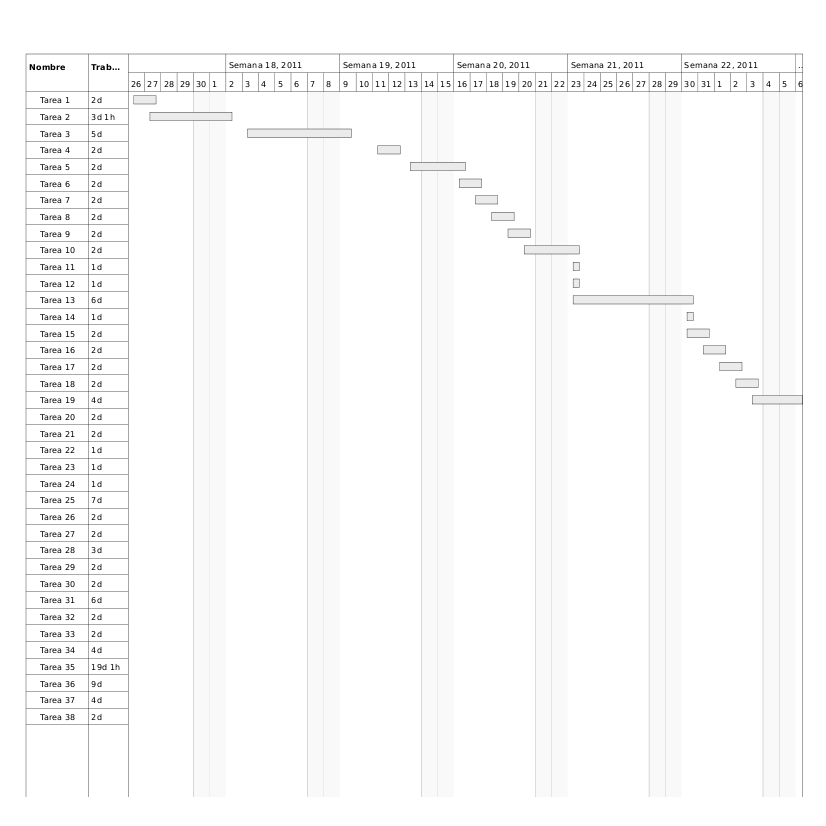
\includegraphics[width=18.5cm]{diagrama_gantt_uno.png}}
\caption{Planificación Temporal del proyecto - Desde el 26 de Abril}
\end{figure}

\pagebreak
\begin{figure}[H]
\hspace*{-.5in}{
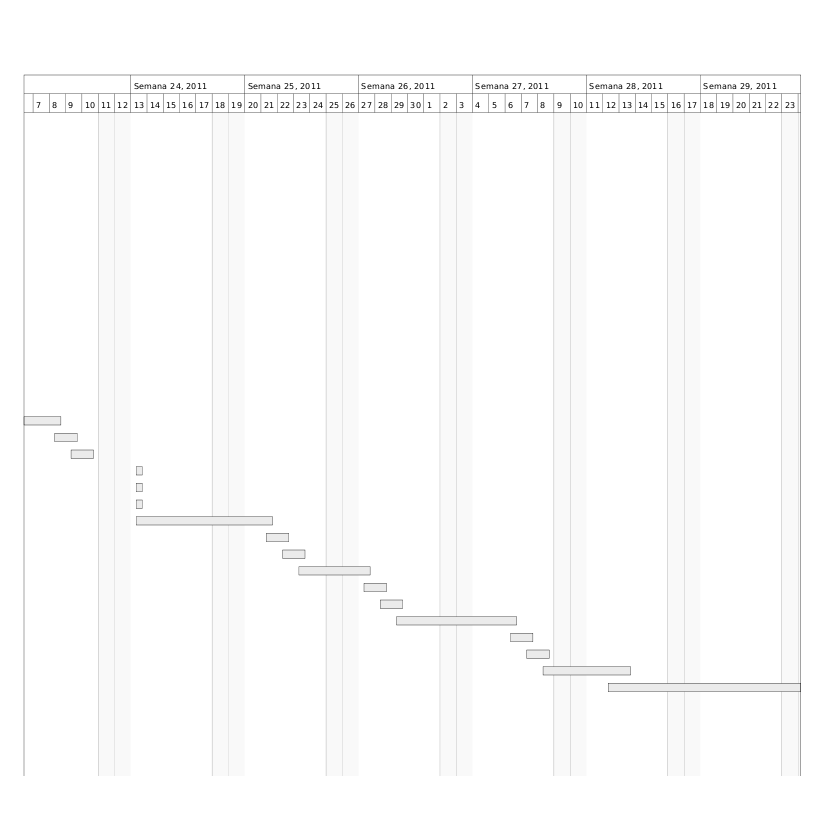
\includegraphics[width=18.5cm]{diagrama_gantt_dos.png}}
\caption{Planificación Temporal del proyecto - Desde el 6 de Junio}
\end{figure}



%\input{pruebas.tex}

\chapter{Guía de usuario}
\label{chap:guía de usuario}

\section{Interfaz gráfica}

Una interfaz gráfica de usuario (GUI) presenta un mecanismo amigable al usuario para interactuar con una aplicación. Una GUI proporciona a una aplicación una ``apariencia visual'' única. Al proporcionar distintas aplicaciones en las que los componentes de la interfaz de usuario sean consistentes e intuitivos, los usuarios pueden familiarizarse en cierto modo con una aplicación, de manera que pueden aprender a utilizarla en menor tiempo y con mayor productividad.\\

Las GUIs se crean a partir de componentes de la GUI. A éstos se les conoce también como controladores o widgets (accesorios de ventana) en otros lenguajes. Un componente de la GUI es un objeto con el cual interactúa el usuario mediante el ratón, el teclado u otra forma de entrada, como el reconocimiento de voz.\\

\section{Componentes GUI en java}

En java existen realmente dos conjuntos de componentes de GUI. Antes de introducir a Swing en Java SE 1.2, las GUIs de Java se creaban a partir de componentes del \textbf{Abstract Window Toolkit (AWT}) en el paquete \textbf{java.awt}. Cuando una aplicación de Java con una GUI del AWT se ejecuta en distintas plataformas, los componentes de la GUI de la aplicación se muestran de manera distinta en cada plataforma. Consideremos una aplicación que muestra un objeto de tipo \emph{Button} (paquete \emph{java.awt}). En una computadora que ejecuta el sistema operativo Microsoft Windows, el objeto \emph{Button} tendrá la misma apariencia que los botones en las demás aplicaciones Windows. De manera similar, en una computadora que ejecuta el sistema operativo Apple Mac OS X, el objeto \emph{Button} tendrá la misma apariencia visual que los botones en las demás aplicaciones Macintosh. Algunas veces, la forma en la que un usuario puede interactuar con un componente específico del AWT difiere entre una plataforma y otra.\\

En conjunto, a la apariencia y la forma en la que interactúa el usuario con la aplicación se les denomina la \textbf{apariencia visual}. Los componentes de GUI de Swing nos permiten especificar una apariencia visual uniforme para una aplicación a través de todas las plataformas, o para usar la apariencia visual personalizada de cada plataforma. Incluso, hasta una aplicación puede modificar la apariencia visual durante la ejecución, para permitir a los usuarios elegir su propia apariencia visual preferida.\\

\section{Introducción}

En este documento se describirá los objetivos e información clara y concisa de cómo utilizar la Suite de Teoría Algorítmica de grafos: Graphvisualx.\\

La Suite de Teoría Algorítmica de grafos: Graphvisualx ha sido creado por Moisés Gautier Gómez para el proyecto de fin de carrera de la titulación de ingeniería informática técnica de sistemas de la universidad de Cádiz. El objetivo es facilitar en la compresión de los estudiantes de la materia de grafos en la resolución de ejemplos de los mismos empleando los algoritmos más conocidos y que usualmente se emplean en el entorno académico.\\

Es de mucha importancia consultar esta guía antes y/o durante la utilización de la Suite, ya que lo guiará paso a paso en el manejo de las funciones de ella. La resolución recomendada para la aplicación debe ser superior o igual a 1024 x 768 (Estándar XGA). \\

Con el fin de facilitar la comprensión de la guía, se incluye gráficos explicativos. Los iconos de la aplicación se han obtenido de la página web \url{http://www.iconfinder.com}. \\

\section{Objetivo de esta guía}

El objetivo primordial de esta guía es ayudar y guiar al usuario a utilizar la Suite de Teoría Algorítmica de grafos: Graphvisualx obteniendo la información adecuada de los algoritmos para despejar todas las dudas existentes y comprende:

\begin{itemize}
\item Guía para acceder a la Suite.
\item Conocer como utilizar la Suite, mediante una descripción detallada e ilustrada de opciones.
\item Conocer el alcance de todos los algoritmos por medio de una explicación detallada de ellos e ilustrada en el manual de algoritmos que se adjuntará en la guía y que también será accesible desde la Suite.
\end{itemize}

\section{Dirigido a}

Esta guía esta dirigida al usuario final de la Suite que utilicen dicho recurso como complemento al material docente de asignaturas de la titulación así como laboratorio de pruebas de algoritmos sobre grafos de ejemplo.

\section{Convenciones y estándares a utilizar}

Entre las convenciones y estándares a utilizar tenemos las siguientes:

\subsection{Convenciones del uso del ratón}

\begin{table}[H]
\begin{tabular}{|p{2cm}|p{3cm}|p{5cm}|p{5cm}|}
\hline
\centering{Término} & \centering{Situación} & \centering{Elemento aplicación} & \qquad \quad Significado \\
\hline
\centering{
\includegraphics[scale=.6]{./imagenes_documentacion/mouse.png}} & - & Sobre cualquier botón & Apertura del menú o acción designado para tal botón. \\
\hline
\multicolumn{4}{|c|}{Modo edición grafo} \\
\hline
\centering{
\includegraphics[scale=.6]{./imagenes_documentacion/mouse_left.png}} & Sobre lienzo de trabajo & Modo crear nodos sobre el lienzo (Botón crear nodo previamente pulsado). & Crea un nodo en el espacio designado para ello. \\
\hline
\centering{
\includegraphics[scale=.6]{./imagenes_documentacion/mouse_right.png}} & Sobre nodo creado en el lienzo de trabajo & Modo crear nodo sobre el lienzo (Botón crear nodo previamente pulsado). & Elimina el nodo creado anteriormente en el nodo. Se reorganiza la numeración del etiquetado de nodos si fuera necesario. \\
\hline
\centering{
\includegraphics[scale=.6]{./imagenes_documentacion/mouse_left.png}} & Sobre un nodo creado y arrastrar el cursor a otro nodo creado. Soltar inmediatamente. & Modo crear arista sobre el lienzo (Botón crear arista previamente pulsado). & Crea una arista de adyacencia (si es dirigido el grafo con la flecha de finalización apuntando hacia el nodo destino) sobre el nodo origen hacia el nodo destino. \\
\hline
\centering{
\includegraphics[scale=.6]{./imagenes_documentacion/mouse_right.png}} & Sobre una arista creada previamente (sobre la etiqueta de ponderación de la misma). & Modo crear arista sobre el lienzo (Botón crear arista previamente pulsado). & Da la opción de modificar el coste/ponderación de la arista o de eliminarla. \\
\hline
\end{tabular}
\end{table}
\newpage
\begin{table}[H]
\begin{tabular}{|p{2cm}|p{3cm}|p{5cm}|p{5cm}|}
\hline
\centering{
\includegraphics[scale=.6]{./imagenes_documentacion/mouse_left.png}} & - & Modo eliminar contenido lienzo. & Elimina todos los elementos contenidos en el lienzo de trabajo. \\
\hline
\centering{
\includegraphics[scale=.6]{./imagenes_documentacion/mouse_both.png}} & Sobre un nodo creado en el lienzo de trabajo & Modo mover nodos (Botón mover nodos previamente pulsado) & Permite cambiar de posición el nodo dentro de lienzo según las preferencias del usuario. \\
\hline
\centering{
\includegraphics[scale=.6]{./imagenes_documentacion/mouse_left.png}} & - & Modo aceptar grafo & Concluye la edición del lienzo de trabajo para la creación de un grafo. \\
\hline
\end{tabular}
\end{table}

\subsection{Convenciones del uso del teclado}

\begin{table}[H]
\begin{center}
\begin{tabular}{|p{6cm}|p{8cm}|}
\hline
\centering{Tecla} & \qquad \quad Significado \\
\hline
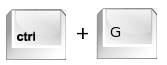
\includegraphics[width=5.5cm]{./imagenes_documentacion/key_ctrl_g.png} & \vspace*{-.8in}{Guardar el grafo inicial. Abre un menú emergente en donde te permite guardar un fichero en formato texto plano en el sistema con el nombre que se desee. No hay que escribir explícitamente la extensión al definir el nombre del fichero, es decir, con escribir ``ejemplo'' el sistema asigna la extensión al nombre inmediatamente.} \\
\hline
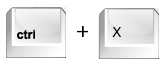
\includegraphics[width=5.5cm]{./imagenes_documentacion/key_ctrl_x.png} & \vspace*{-.8in}{Salir de la Suite. Cierra la Suite y para volver a acceder a ella se tendrá que hacer doble clic sobre el lanzador.} \\
\hline
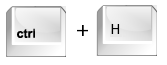
\includegraphics[width=5.5cm]{./imagenes_documentacion/key_ctrl_h.png} & \vspace*{-.8in}{Guía del usuario. Se abre una nueva ventana en donde vendrá definida la guía del usuario para cualquier duda sobre el uso de Graphvisualx.} \\
\hline
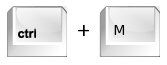
\includegraphics[width=5.5cm]{./imagenes_documentacion/key_ctrl_m.png} & \vspace*{-.8in}{Manual de los algoritmos y conceptos relacionados con la teoría algorítmica de grafos. Se abre una nueva ventana en donde vendrá definido un documento en formato pdf con los contenidos teóricos necesarios en caso de duda.} \\
\hline
\end{tabular}
\end{center}
\end{table}
\newpage
\begin{table}[H]
\begin{center}
\begin{tabular}{|p{6cm}|p{8cm}|}
\hline
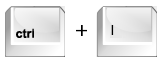
\includegraphics[width=5.5cm]{./imagenes_documentacion/key_ctrl_i.png} & \vspace*{-.8in}{Sobre Graphvisualx. Se abre una nueva ventana donde viene información sobre el autor de Graphvisualx y demás.} \\
\hline
\end{tabular}
\end{center}
\end{table}

\section{Ingreso al sistema}

Una vez descargada la aplicación y colocada en el directorio deseado hacemos doble clic sobre ella para ejecutar la Suite. Sino se produciese ningún evento probar con la siguiente opción:
\begin{figure}[H]
\hspace*{-.75in}{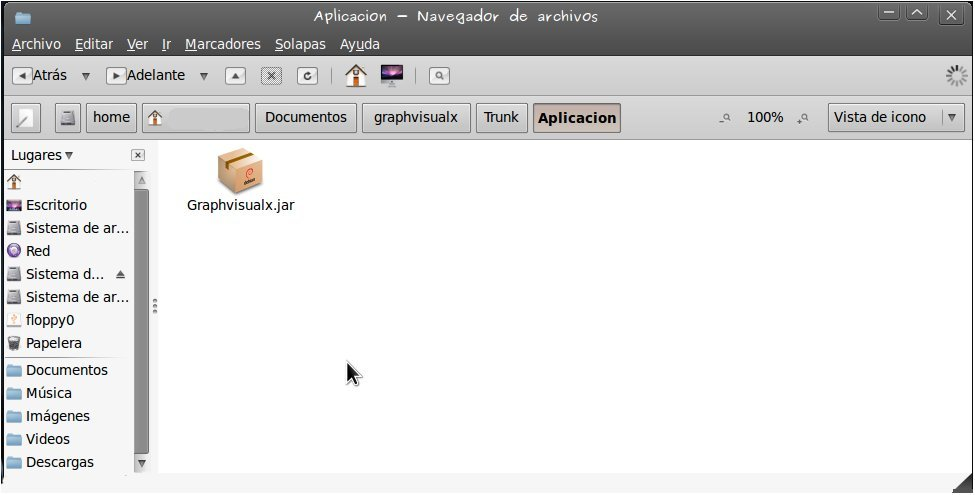
\includegraphics[width=20cm]{./imagenes_documentacion/captura_1.jpeg}}
\caption{Directorio de trabajo donde se encuentra el fichero .jar ejecutable de la Suite.}
\end{figure}
\newpage
\begin{figure}[H]
\hspace*{.5in}{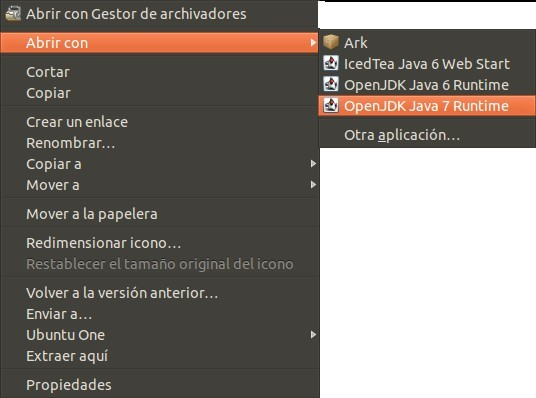
\includegraphics[width=13cm]{./imagenes_documentacion/desplegable_menu_abrir_jar.jpeg}}
\caption{Menú desplegable al pulsar botón derecho sobre el ejecutable .jar y selección de programa.}
\end{figure}

\subsection{Como acceder a la suite}
\label{cap:Acceder}

Si no se dispusiese de máquina virtual java en el sistema se deberá instalar a través de línea de comandos en el terminal de GNU/Linux.
Para ello primeramente hay que escribir \url{http://www.java.com/es/download/help/linux_install.xml} en nuestro navegador favorito para ir a la página web de java, en donde se nos explica el método de instalación a seguir. Sea pues:
\newpage
\begin{figure}[H]
\hspace*{-.8in}{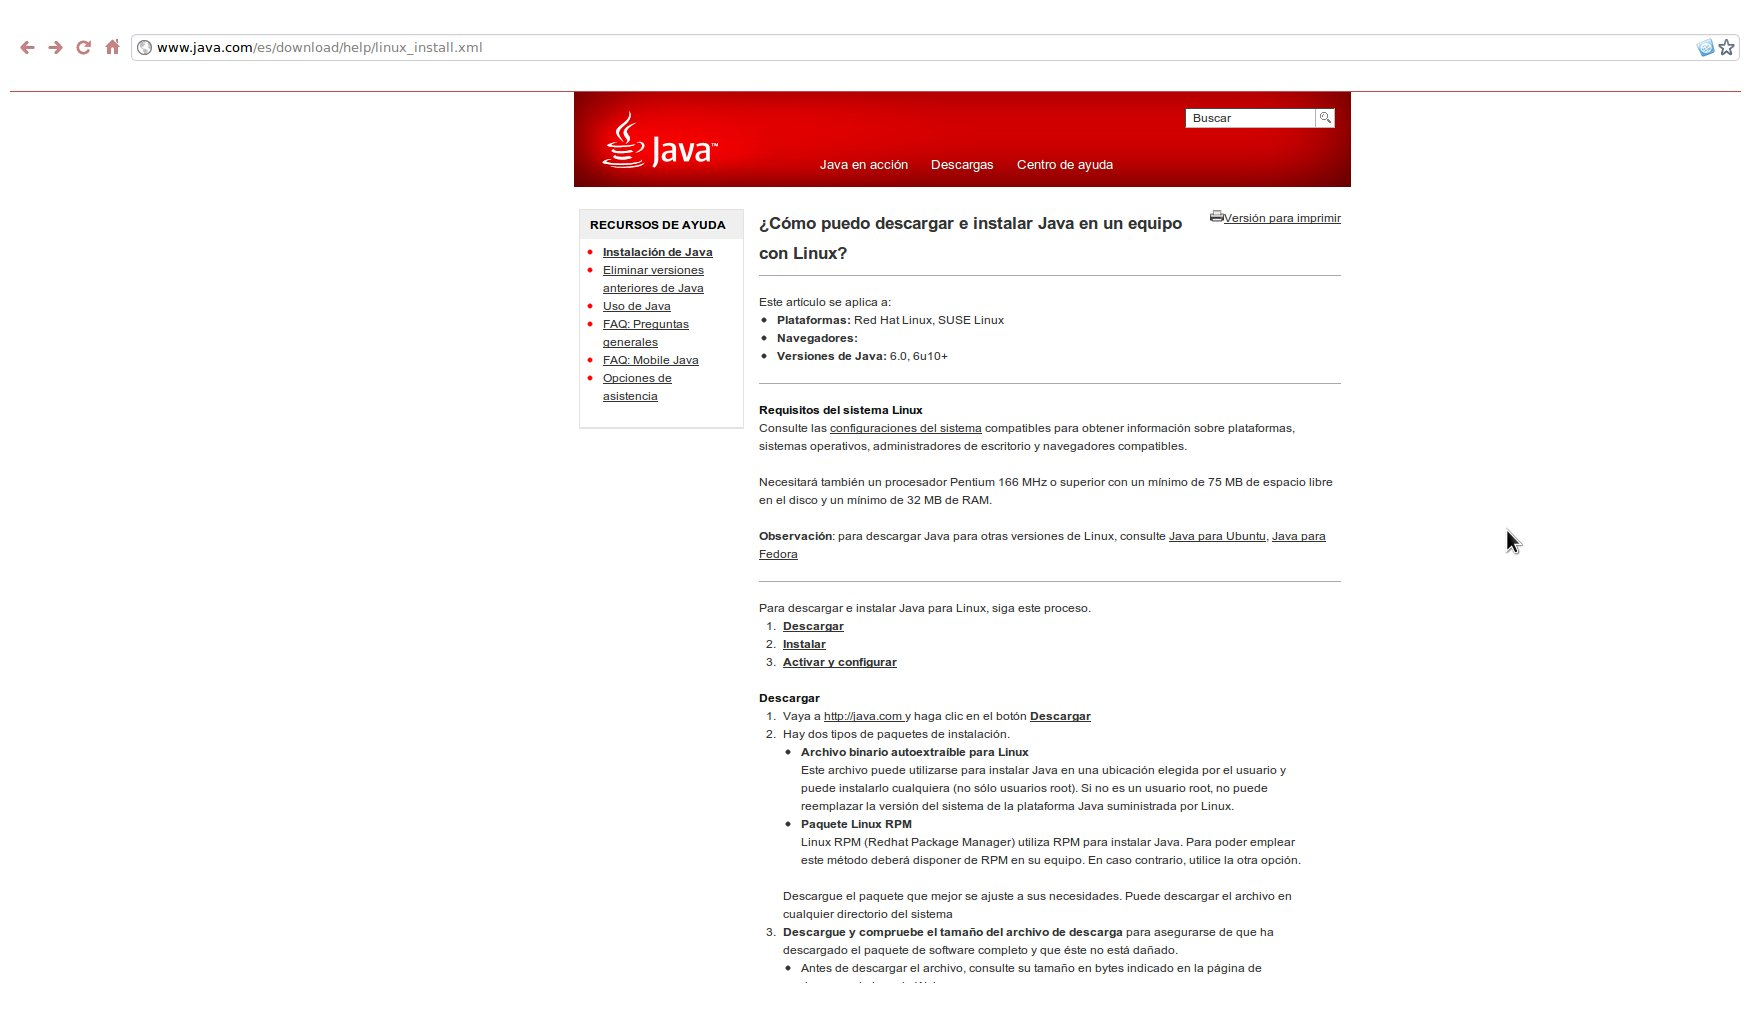
\includegraphics[width=20cm]{./imagenes_documentacion/captura_2.jpeg}}
\caption{Página web de Java donde se explican los pasos para la instalación del software Java en nuestro sistema GNU/Linux.}
\end{figure}

\begin{figure}[H]
\hspace*{-.8in}{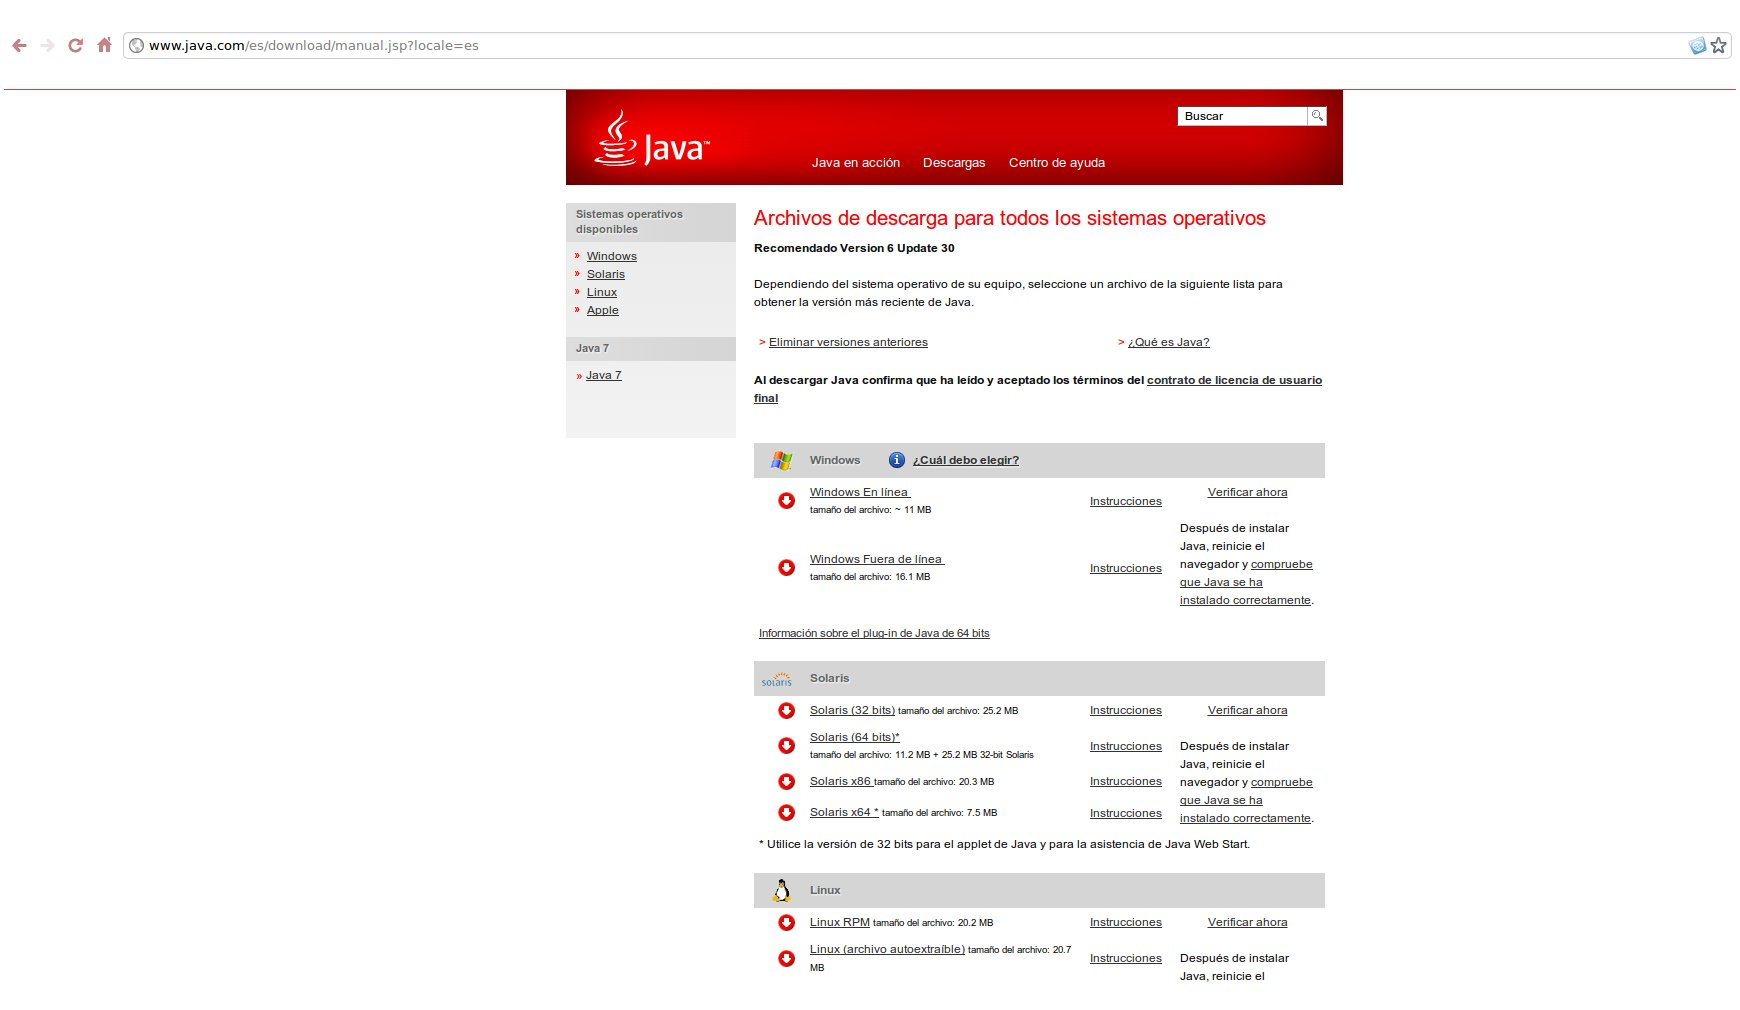
\includegraphics[width=20cm]{./imagenes_documentacion/captura_3.jpeg}}
\caption{Página web donde se encuentran los ficheros descargables según sistema operativo \url{http://www.java.com/es/download/manual.jsp?locale=es}.}
\end{figure}

\begin{figure}[H]
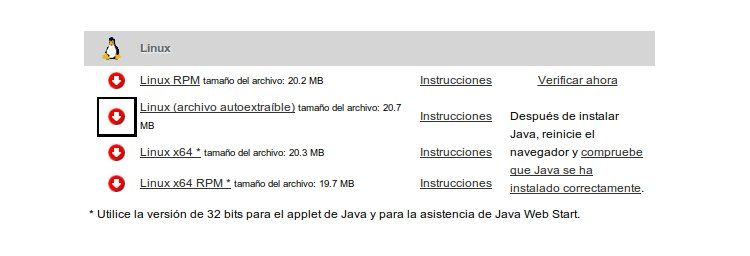
\includegraphics[width=15cm]{./imagenes_documentacion/captura_4.jpeg}
\caption{Sección de la página web de la figura 7.4 en donde se especifica para el sistema operativo GNU/Linux.}
\end{figure}

Si se desea la descarga del archivo en formato ``.rpm'' se deberá poner en la línea de comandos para su instalación el comando:\\

\begin{center} \emph{rpm -Uvh nombre\_paquete.rpm}\\ \end{center}

Si por el contrario se descarga el fichero en formato autoextraible será necesario escribir el siguiente comando en la línea de comandos:\\

\begin{center} \emph{sh nombre\_paquete.bin}\\ \end{center}

Además de todo ello se deberá tener instalado también el jdk de java para poder visualizar la aplicación perfectamente en nuestro sistema. Para ello tenemos que teclear en línea de comandos:\\
\begin{center} \emph{sudo apt-get install openjdk-jre} \\ \end{center}

\subsection{Problemas con los permisos de la aplicación}

Hay veces en las que la generación de documentos en un sistema GNU/Linux sigue las directrices de la función/orden umask que establece los permisos por defecto de todos los nuevos ficheros en el sistema de archivos. Según sea el caso nuestro sistema puede no ser capaz de realizar la ejecución de la aplicación por la falta de alguno de los permisos necesarios.\\

\begin{figure}[H]
\begin{center}
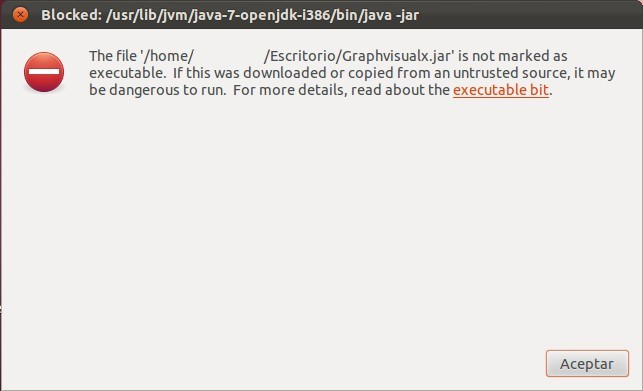
\includegraphics[width=16cm]{./imagenes_documentacion/captura_error_ejecucion_jar.jpeg}
\caption{Mensaje de error al no tener habilitados los permisos de ejecución la aplicación.}
\end{center}
\end{figure}

Para ello será necesario posicionarse en el directorio donde se encuentre la aplicación, a través de una terminal/consola en nuestro sistema GNU/Linux favorito, y teclear el siguiente comando:\\

\begin{center} \emph{chmod +x Graphvisualx.jar} \\ \end{center}

\subsection{Paquetes adicionales para distribuciones GNU/Linux}

Para la generación de los ficheros en formato imagen de los grafos es necesario instalar en su sistema el paquete graphviz, que es un software de código abierto empleado en la visualización de grafos. Sin este software el fichero generado por el módulo de la aplicación (Graphviz.java) en formato .dot no puede ser interpretado por el sistema para su posterior transformación a imagen visual.\\

Nos dirigimos a una terminal en donde debemos introducir el siguiente comando:

\begin{center} \emph{sudo apt-get install graphviz} \\ \end{center}

Por motivos de eficiencia el algoritmo de compresión de imágenes será .png dado que es muy práctico y extendido para imágenes que no requieran de un alto contenido de detalles, conservando todos los colores posibles.

\section{Operaciones de la suite}
\subsection{Archivo}

Icono representativo: 
\includegraphics[scale=.7]{./imagenes_documentacion/archivo.png} \\

Dentro de este apartado se definirán los items del menú de archivo. En él se encuentran cuatro posibles operaciones a realizar por el usuario según haya o no:
\begin{itemize}
\item Creado un grafo mediante su edición o cargado en el sistema.
\item Procesado dicho grafo mediante algún algoritmo.
\item En caso contrario, no haber realizado ninguna operación con el sistema.
\end{itemize}

Para el caso de que el usuario haya simplemente cargado o editado un grafo en el sistema, tendrá las siguientes operaciones disponibles (o items) del menú archivo.

\begin{itemize}
\item Guardar grafo inicial (Atajo de teclado Ctrl+g). \quad 
\includegraphics[scale=.9]{./imagenes_documentacion/guardar.png} 
\item Guardar grafo como imagen. \quad 
\includegraphics[scale=.15]{./imagenes_documentacion/guardar_imagen.png}
\item Salir (Atajo de teclado Ctrl+x). \quad 
\includegraphics[scale=.9]{./imagenes_documentacion/exit.png}
\end{itemize}

Cuando el usuario haya procedo un grafo, previamente definido en el sistema, con uno de los algoritmos posibles tendrá las siguientes operaciones disponibles (o items) del menú archivo.

\begin{itemize}
\item Guardar grafo inicial (Atajo de teclado Ctrl+g). \quad 
\includegraphics[scale=.9]{./imagenes_documentacion/guardar.png} 
\item Guardar grafo como imagen. \quad 
\includegraphics[scale=.15]{./imagenes_documentacion/guardar_imagen.png}
\item Guardar grafo resultado como imagen. \quad 
\includegraphics[scale=.15]{./imagenes_documentacion/guardar_imagen.png}
\item Salir (Atajo de teclado Ctrl+x). \quad 
\includegraphics[scale=.9]{./imagenes_documentacion/exit.png}
\end{itemize}

En caso contrario de no haber realizado ninguna operación con el sistema, tendrá las siguientes operaciones disponibles (o items) del menú archivo.

\begin{itemize}
\item Salir (Atajo de teclado Ctrl+x). \quad 
\includegraphics[scale=.9]{./imagenes_documentacion/exit.png}
\end{itemize}

Guardar grafo inicial permite al usuario, una vez haya realizado la edición o creación de un nuevo grafo en el sistema, guardar la estructura interna del grafo en un fichero en formato de texto plano en su sistema de ficheros para posteriormente simplemente cargar dicho fichero sin necesidad de editar de nuevo todo su contenido. No es necesario establecer la extensión de ``.txt'' al nombre del archivo, ya que automáticamente el sistema dota de tal extensión al nombre adjunto. Su atajo de teclado es: Ctrl+G. \\

\begin{figure}[H]
\begin{center}
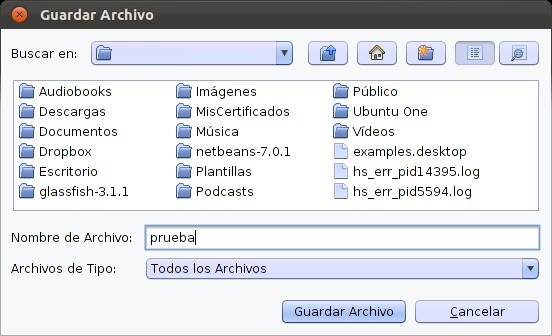
\includegraphics[width=13cm]{./imagenes_documentacion/imagen_guardar_archivo.jpeg}
\caption{Listado de directorios donde se puede seleccionar el destino del archivo.}
\end{center}
\end{figure}

Guardar grafo como imagen permite al usuario, una vez haya realizado la edición o creación de un nuevo grafo en el sistema, guardar la estructura visual del grafo en un fichero en formato imagen (png) en su sistema de ficheros para posteriormente usarla como material adicional de un trabajo o simplemente para almacenar de una manera visual dicho contenido en vez del fichero de texto plano. Esta opción no permite guardar el grafo para posteriores cargas en el sistema, ya que simplemente se limita a crear una representación con graphviz del contenido del grafo. En ningún momento se almacena la estructura del mismo adjunta a la imagen. Para ello es necesario usar la opción anterior de ``Guardar grafo inicial''.\\

\begin{figure}[H]
\begin{center}
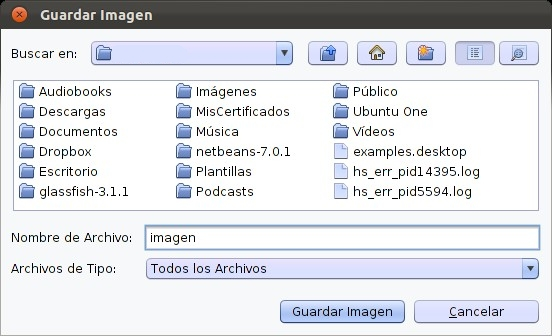
\includegraphics[width=13cm]{./imagenes_documentacion/imagen_guardar_imagen.jpeg}
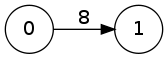
\includegraphics[width=3cm]{./imagenes_documentacion/grafo.png}
\caption{Listado de directorios donde se puede seleccionar el destino del archivo e imagen resultante.}
\end{center}
\end{figure}

Guardar grafo resultado como imagen permite al usuario, una vez haya realizado algún procesamiento sobre un grafo del sistema, guardar la estructura visual del grafo resultado del procesamiento en un fichero en formato imagen (png) en su sistema de ficheros para posteriormente usarla como material adicional de un trabajo o simplemente para almacenar de una manera visual dicho resultado. \\

Salir, según su nombre indica, permite al usuario abandonar la aplicación. Su atajo de teclado es: Ctrl+x. \\
\subsection{Ayuda}

Icono representativo: 
\includegraphics[scale=.2]{./imagenes_documentacion/ayuda.png} \\

Dentro de este apartado se definirán los items del menú de ayuda. En él se encuentran tres posibles operaciones de consulta para el usuario.
\begin{itemize}
\item Guía de uso (Atajo de teclado Ctrl+h). \quad 
\includegraphics[scale=.95]{./imagenes_documentacion/guide.png}
\item Algoritmos y conceptos (Atajo de teclado Ctrl+m). \quad 
\includegraphics[scale=.9]{./imagenes_documentacion/manual.png}
\item Sobre Graphvisualx (Atajo de teclado Ctrl+I). \quad 
\includegraphics[scale=.9]{./imagenes_documentacion/about.png}
\end{itemize}

La guía de uso servirá para solventar las dudas de uso de la aplicación. En ella se hará un recorrido por todas las funcionalidades de la suite, así como los posibles usos que tiene cada componente de la misma. Su atajo de teclado es: Ctrl+h. \\

En el menú de algoritmos y conceptos se describe paso a paso, para los casos descritos, los conceptos y algoritmos usados para la Suite informática de Teoría Algorítmica de Grafos. Se hará uso de trazas en ciertos casos y su representación en formato código java en la que se basa la suite. Su atajo de teclado es: Ctrl+m. \\

\begin{figure}[H]
\begin{center}
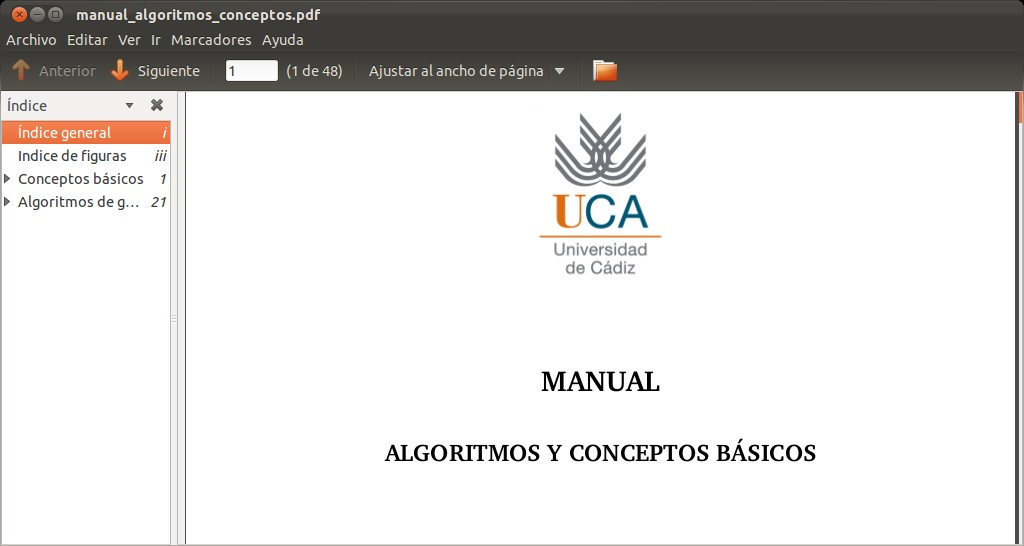
\includegraphics[width=17cm]{./imagenes_documentacion/imagen_manual_algoritmos.jpeg}
\caption{Ventana donde se encuentran disponibles todos los algoritmos de la suite para lectura.}
\end{center}
\end{figure}


Por último en el menú titulado ``sobre Graphvisualx'', se hace una breve mención sobre el creador del proyecto, el nombre del mismo y para la universidad que ha sido desarrollada la aplicación. Su atajo de teclado es: Ctrl+i. \\

\begin{figure}[H]
\begin{center}
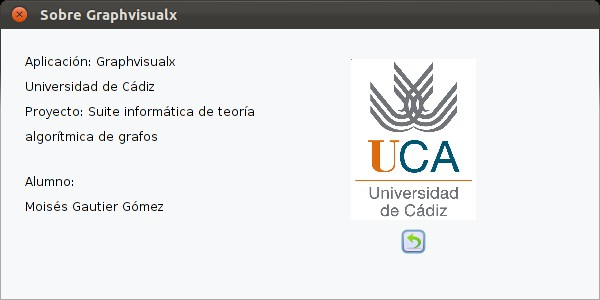
\includegraphics[width=17cm]{./imagenes_documentacion/imagen_sobre_graphvisualx.jpeg}
\caption{Ventana donde se visualiza la información relacionada con Graphvisualx.}
\end{center}
\end{figure}

\subsection{Creación grafo}

Grupo de iconos representativos: \icontext{0.4}{0.7}{./imagenes_documentacion/imagen_creacion_grafo.jpeg} \\

Este grupo de botones permiten la siguiente funcionalidad:

\begin{itemize}
\item Nuevo grafo. \quad \icontext{.4}{.9}{./imagenes_documentacion/nuevo.png}
\item Cargar fichero. \quad \icontext{.4}{.9}{./imagenes_documentacion/cargar.png}
\item Aplicar algoritmo. \quad \icontext{.4}{.9}{./imagenes_documentacion/algoritmos.png}
\end{itemize}

Con el botón de nuevo grafo el sistema abre la edición de un nuevo panel o lienzo para que el usuario edite o cree un grafo según los nodos y aristas que desee. Para el caso de las aristas se empleará un sistema de ponderación (etiquetado de las mismas) que se encuentran dentro del dominio de los números enteros.  \\

Cargar fichero permite al usuario cargar desde el propio sistema de ficheros sobre el que trabaje, la introducción de una estructura de tipo grafo almacenada a tal efecto en formato de texto plano. Previamente debería de haberse guardado usando la opción de ``Guardar grafo inicial'' disponible dentro del menú Archivo. \\

Por último se encuentra la opción de aplicar algoritmo que permitirá al usuario desplegar la funcionalidad de la suite para el grafo que se haya editado o cargado previamente en el sistema. Esta opción se encontrará disponible, única y exclusivamente, cuando el usuario haya realizado una carga exitosa de un fichero con la estructura de grafo o cuando haya aceptado el grafo editado en el lienzo de trabajo. En los demás casos esta opción se encontrará deshabilitada. \\

\subsection{Edición grafo}

Grupo de iconos representativos: \icontext{0.4}{0.7}{./imagenes_documentacion/imagen_edicion_grafo.jpeg} \\

Este grupo de botones permiten la siguiente funcionalidad:

\begin{itemize}
\item Crear nodo. \quad \icontext{.4}{.7}{./imagenes_documentacion/nodo.png}
\item Crear arista. \quad \icontext{.4}{.7}{./imagenes_documentacion/arista.png}
\item Borrar contenido lienzo. \quad \icontext{.4}{.7}{./imagenes_documentacion/eraser.png}
\item Mover nodos. \quad \icontext{.4}{.7}{./imagenes_documentacion/mover.png}
\item Aceptar grafo. \quad \icontext{.4}{.7}{./imagenes_documentacion/aceptar.png}
\end{itemize}

Crear nodo permite al usuario la edición de los nodos que desee, en el lienzo de trabajo del grafo dispuesto justo abajo del grupo de botones. Al hacer clic izquierdo se creará un nodo etiquetado según haya o no alguno ya anterior en el lienzo. Por defecto el primer nodo será $0$ y así sucesivamente $0,\ 1,\ 2,\ 3,\ \ldots,\ n$ donde $n \in \mathbb{N}$. Por el contrario al realizar clic derecho sobre un nodo \textbf{previamente creado} en el lienzo de trabajo, este se eliminará de la estructura interna y los demás nodos serán re-etiquetados en respectivo orden. \\

\begin{figure}[H]
\begin{center}
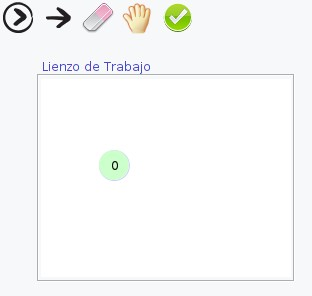
\includegraphics[width=10cm]{./imagenes_documentacion/imagen_nodo_creado_lienzo.jpeg}
\caption{Resultado de hacer clic izquierdo sobre el lienzo una vez se ha seleccionado la opción de crear nodo.}
\end{center}
\end{figure}

Crear arista permite al usuario la edición, sobre los nodos origen y destino que desee, de una arista en el lienzo de trabajo del grafo dispuesto justo abajo del grupo de botones. Es importante tomar constancia que la arista se creará si se realiza un primer clic izquierdo sobre un nodo y posteriormente arrastramos el puntero del ratón hasta soltarlo dentro de otro nodo destino, en caso contrario no sucederá ningún evento asociado. Una vez hayamos hecho clic y luego arrastrado la arista hasta otro nodo, se abrirá una venta emergente en donde podremos introducir el valor asociado a la arista sea dirigida o no. El rango de valores posibles de pesos dentro de la arista esta encuadrado en el dominio de los números enteros con límite superior de $100$ e inferior de $-100$. \\

\begin{figure}[H]
\begin{center}
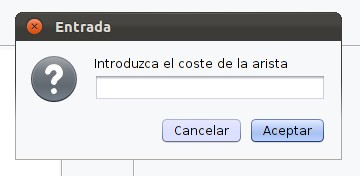
\includegraphics[width=8cm]{./imagenes_documentacion/imagen_valor_arista.jpeg}
\caption{Ventana para introducir el coste de una arista.}
\end{center}
\end{figure}

Una vez que se haya creado la arista podemos realizar estas dos siguientes operaciones si hacemos clic derecho sobre el trozo de la derecha, a partir de la etiqueta, de la arista.

\begin{itemize}
\item Borrar arista. 
\item Modificar coste.
\end{itemize}
 
\begin{figure}[H]
\begin{center}
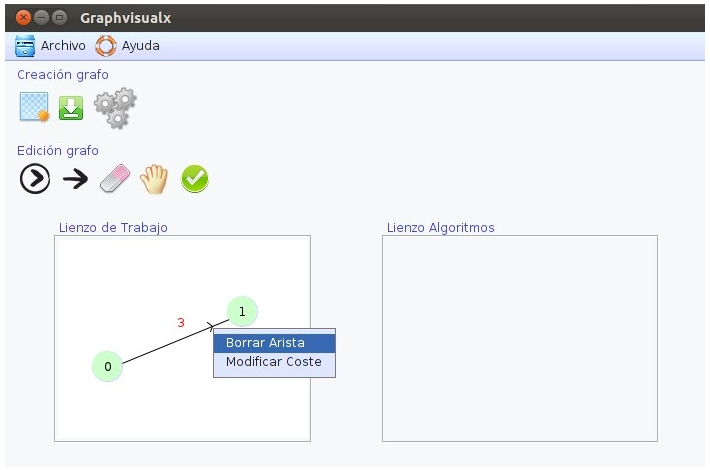
\includegraphics[width=15cm]{./imagenes_documentacion/imagen_nodos_con_arista_opcion_arista_modificada.jpeg}
\caption{Resultado al hacer clic derecho sobre la arista.}
\end{center}
\end{figure}

Borrar arista, como su nombre indica, elimina la arista que une los nodos origen y destino visualmente además de manera interna en la estructura.\\

Modificar coste permite al usuario rectificar un valor asociado al peso o etiquetado de la arista. \\

\newpage

\begin{figure}[H]
\begin{center}
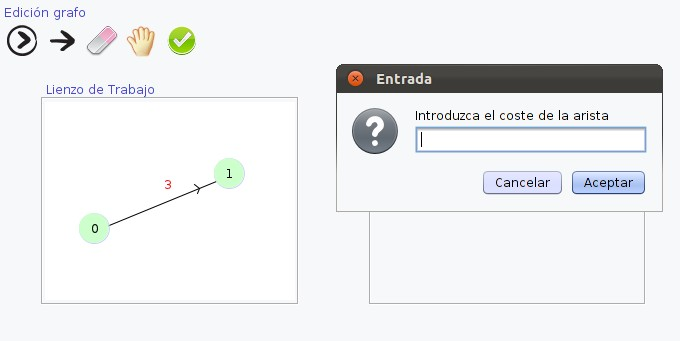
\includegraphics[width=17cm]{./imagenes_documentacion/imagen_icono_modificar_arista.jpeg}
\caption{Resultado de seleccionar la opción de modificar arista en el menú emergente.}
\end{center}
\end{figure}

\subsection{Propiedades del grafo}

Todos los grafos que se pueden tanto editar como cargar en el sistema tienen una serie de propiedades innatas en el cuerpo matemático de los grafos, tales como linealidad, completitud, sentido de la navegabilidad, adyacencia, etc. Dichas propiedades serán visibles para cada grafo (lienzo donde se muestre el grafo tanto inicial como resultado) al realizar la operación de aceptado del grafo tanto en el lienzo de trabajo como al aplicar cualquiera de los algoritmos disponibles del sistema. \\

\begin{figure}[H]
\begin{center}
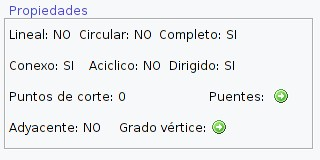
\includegraphics[width=10cm]{./imagenes_documentacion/imagen_propiedades_grafo.jpeg}
\caption{Bloque de contenidos situado abajo de los lienzos donde se visualizan las propiedades de los grafos.}
\end{center}
\end{figure}

Dentro de las propiedades del grafo se encuentran disponibles dos botones: uno tendrá la funcionalidad de hallar el grado del vértice que el usuario desee introduciendo dicho vértice en la ventana emergente a tal efecto y luego hay otro donde permitirá al usuario visualizar, si fuera el caso, los puentes que posee dicho grafo editado en el lienzo de trabajo o cargado en el sistema a través de un fichero. El resultado al pulsar el botón de puentes será visualizado en el lienzo resultado de grafos. \\

\begin{figure}[H]
\begin{center}
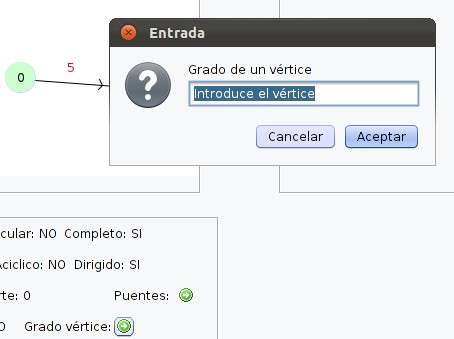
\includegraphics[width=10cm]{./imagenes_documentacion/imagen_grado_vertice_grafo.jpeg}
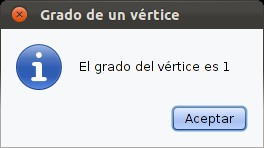
\includegraphics[width=6cm]{./imagenes_documentacion/imagen_grado_grafo_ventana.jpeg}
\caption{Ventana emergente al seleccionar el botón de grado del vértice para el grafo del lienzo.}
\end{center}
\end{figure}

\newpage
\subsection{Algoritmos de grafos}

Finalmente llegamos a la parte principal de la aplicación y así como de procesamiento de los grafo en el sistema. A continuación se muestra una primera captura de la ventana en donde se encuentran establecidos los distintos algoritmos del sistema. 

\begin{figure}[H]
\begin{center}
\hspace*{-.25in}{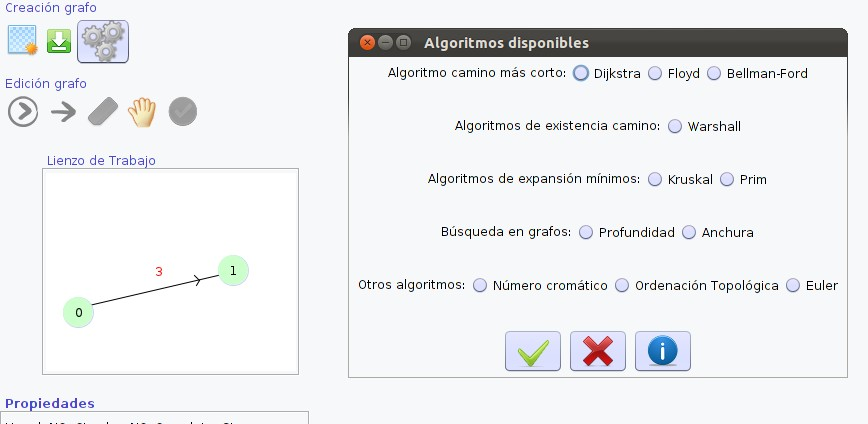
\includegraphics[width=17cm]{./imagenes_documentacion/imagen_icono_algoritmos_ventana_resultante.jpeg}}
\caption{Vista general de la ventana de aplicación de algoritmos sobre el grafo creado.}
\end{center}
\end{figure}

El primer algoritmo disponible, para el procesamiento del camino más corto, es el de Dijkstra \ref{sec:dijkstra}.
\newpage
\begin{figure}[H]
\begin{center}
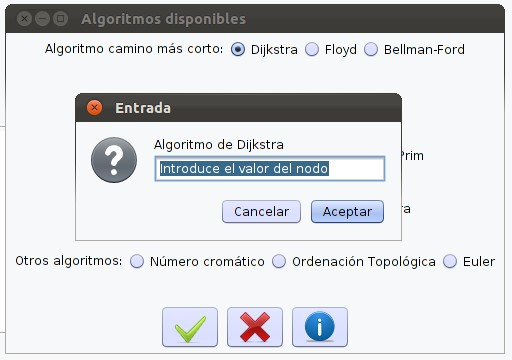
\includegraphics[width=10cm]{./imagenes_documentacion/imagen_icono_dijkstra_ventana_datos.jpeg}
\caption{Ventana emergente de la primera interacción con el algoritmo de Dijkstra.}
\vspace*{.2in}{\includegraphics[width=16cm]{./imagenes_documentacion/imagen_resultado_dijkstra_vertice_0.jpeg}}
\caption{Resultado en el lienzo resultado al aplicar sobre el grafo inicial el algoritmo de Dijkstra.}
\end{center}
\end{figure}

\newpage
El segundo algoritmo, también empleado para el procesamiento del camino más corto, es el de Floyd \ref{sec:floyd}.

\begin{figure}[H]
\begin{center}
\includegraphics[width=10cm]{./imagenes_documentacion/imagen_resultado_floyd.jpeg}
\caption{Resultado en el lienzo resultado al aplicar sobre el grafo inicial el algoritmo de Floyd.}
\end{center}
\end{figure}

El tercer algoritmo, también empleado para el procesamiento del camino más corto, es el de Bellman-Ford \ref{sec:bellman}. Este algoritmo tiene la peculiaridad de que la ponderación de sus aristas pueden ser de coste tanto negativo como positivo, dentro del domino de los números enteros. Además la suma de los flujos o pesos desde el vértice origen hasta el nodo destino se irán mostrando como pesos asociados al camino posible desde el nodo origen establecido.
\newpage
\begin{figure}[H]
\begin{center}
\includegraphics[width=11cm]{./imagenes_documentacion/imagen_bellman_ford_ventana_datos.jpeg}
\caption{Ventana emergente de la primera interacción con el algoritmo de Bellman-Ford.}
\end{center}
\end{figure}

\begin{figure}[H]
\begin{center}
\includegraphics[width=10cm]{./imagenes_documentacion/imagen_resultado_bellman_ford_vertice_0.jpeg}
\caption{Resultado en el lienzo resultado al aplicar sobre el grafo inicial el algoritmo de Bellman-Ford.}
\end{center}
\end{figure}
\newpage
El cuarto algoritmo disponible, que permite averiguar los caminos posibles entre todos los nodos, es Warshall \ref{sec:warshall}.

\begin{figure}[H]
\begin{center}
\includegraphics[width=10cm]{./imagenes_documentacion/imagen_warshall_y_resultado.jpeg}
\caption{Resultado en el lienzo resultado al aplicar sobre el grafo inicial el algoritmo de Warshall.}
\end{center}
\end{figure}

El quinto algoritmo disponible permite obtener el árbol de expansión de coste mínimo para el algoritmo de Kruskal \ref{sec:kruskal}.

\begin{figure}[H]
\begin{center}
\includegraphics[width=10cm]{./imagenes_documentacion/imagen_kruskal_y_resultado.jpeg}
\caption{Resultado en el lienzo resultado al aplicar sobre el grafo el algoritmo de Kruskal.}
\end{center}
\end{figure}
\newpage
El sexto algoritmo disponible permite obtener el árbol de expansión de coste mínimo para el algoritmo de Prim \ref{sec:prim}.

\begin{figure}[H]
\begin{center}
\includegraphics[width=10cm]{./imagenes_documentacion/imagen_prim_y_resultado.jpeg}
\caption{Resultado en el lienzo resultado al aplicar sobre el grafo el algoritmo de Kruskal.}
\end{center}
\end{figure}

El séptimo algoritmo disponible permite el recorrido en anchura del grafo \ref{sec:anchura}.

\begin{figure}[H]
\begin{center}
\includegraphics[width=10cm]{./imagenes_documentacion/imagen_anchura_y_resultado.jpeg}
\caption{Resultado en el lienzo resultado al aplicar sobre el grafo el algoritmo de recorrido en anchura.}
\end{center}
\end{figure}
\newpage
El octavo algoritmo disponible permite el recorrido en profundidad del grafo \ref{sec:profundidad}.

\begin{figure}[H]
\begin{center}
\includegraphics[width=10cm]{./imagenes_documentacion/imagen_profundidad_y_resultado.jpeg}
\caption{Resultado en el lienzo resultado al aplicar sobre el grafo el algoritmo de recorrido en profundidad.}
\end{center}
\end{figure}

El noveno algoritmo disponible permite obtener el número cromático del grafo \ref{sec:cromatico}.

\begin{figure}[H]
\begin{center}
\includegraphics[width=10cm]{./imagenes_documentacion/imagen_numero_cromatico.jpeg}
\caption{Resultado en una ventana emergente donde se dice aproximadamente el número cromático.}
\end{center}
\end{figure}
\newpage
El décimo algoritmo disponible permite obtener la ordenación topológica del grafo \ref{sec:topologico}. El grafo en esta ocasión es distinto al anteriormente usado dado que el anterior al contener una sola arista no mostraba dicha ordenación trivial. \\

\begin{figure}[H]
\begin{center}
\includegraphics[width=13cm]{./imagenes_documentacion/imagen_ordenacion_topologica_y_resultado.jpeg}
\caption{Resultado en el lienzo resultado al aplicar sobre el grafo el algoritmo de Ordenación topológica.}
\end{center}
\end{figure}

Para concluir los algoritmos disponibles tenemos el algoritmo de Euler \ref{sec:euler}.

\begin{figure}[H]
\begin{center}
\includegraphics[width=10cm]{./imagenes_documentacion/imagen_euler.jpeg}
\caption{Resultado en el lienzo resultado al aplicar sobre el grafo el algoritmo de Euler.}
\end{center}
\end{figure}



\backmatter

\clearpage
\nocite{*}
\bibliographystyle{plain}
\bibliography{biblio}
\pagestyle{empty}



\chapter{GNU Documentation Free License}
\label{chap:fdl}


\phantomsection  % so hyperref creates bookmarks

 \begin{center}

       Version 1.3, 3 November 2008


 Copyright \copyright{} 2000, 2001, 2002, 2007, 2008  Free Software Foundation, Inc.
 
 \bigskip
 
     <\url{http://fsf.org/}>
  
 \bigskip
 
 Everyone is permitted to copy and distribute verbatim copies
 of this license document, but changing it is not allowed.
\end{center}


\begin{center}
{\bf\large Preamble}
\end{center}

The purpose of this License is to make a manual, textbook, or other
functional and useful document ``free'' in the sense of freedom: to
assure everyone the effective freedom to copy and redistribute it,
with or without modifying it, either commercially or noncommercially.
Secondarily, this License preserves for the author and publisher a way
to get credit for their work, while not being considered responsible
for modifications made by others.

This License is a kind of ``copyleft'', which means that derivative
works of the document must themselves be free in the same sense.  It
complements the GNU General Public License, which is a copyleft
license designed for free software.

We have designed this License in order to use it for manuals for free
software, because free software needs free documentation: a free
program should come with manuals providing the same freedoms that the
software does.  But this License is not limited to software manuals;
it can be used for any textual work, regardless of subject matter or
whether it is published as a printed book.  We recommend this License
principally for works whose purpose is instruction or reference.


\begin{center}
{\Large\bf 1. APPLICABILITY AND DEFINITIONS\par}
\end{center}

This License applies to any manual or other work, in any medium, that
contains a notice placed by the copyright holder saying it can be
distributed under the terms of this License.  Such a notice grants a
world-wide, royalty-free license, unlimited in duration, to use that
work under the conditions stated herein.  The ``\textbf{Document}'', below,
refers to any such manual or work.  Any member of the public is a
licensee, and is addressed as ``\textbf{you}''.  You accept the license if you
copy, modify or distribute the work in a way requiring permission
under copyright law.

A ``\textbf{Modified Version}'' of the Document means any work containing the
Document or a portion of it, either copied verbatim, or with
modifications and/or translated into another language.

A ``\textbf{Secondary Section}'' is a named appendix or a front-matter section of
the Document that deals exclusively with the relationship of the
publishers or authors of the Document to the Document's overall subject
(or to related matters) and contains nothing that could fall directly
within that overall subject.  (Thus, if the Document is in part a
textbook of mathematics, a Secondary Section may not explain any
mathematics.)  The relationship could be a matter of historical
connection with the subject or with related matters, or of legal,
commercial, philosophical, ethical or political position regarding
them.

The ``\textbf{Invariant Sections}'' are certain Secondary Sections whose titles
are designated, as being those of Invariant Sections, in the notice
that says that the Document is released under this License.  If a
section does not fit the above definition of Secondary then it is not
allowed to be designated as Invariant.  The Document may contain zero
Invariant Sections.  If the Document does not identify any Invariant
Sections then there are none.

The ``\textbf{Cover Texts}'' are certain short passages of text that are listed,
as Front-Cover Texts or Back-Cover Texts, in the notice that says that
the Document is released under this License.  A Front-Cover Text may
be at most 5 words, and a Back-Cover Text may be at most 25 words.

A ``\textbf{Transparent}'' copy of the Document means a machine-readable copy,
represented in a format whose specification is available to the
general public, that is suitable for revising the document
straightforwardly with generic text editors or (for images composed of
pixels) generic paint programs or (for drawings) some widely available
drawing editor, and that is suitable for input to text formatters or
for automatic translation to a variety of formats suitable for input
to text formatters.  A copy made in an otherwise Transparent file
format whose markup, or absence of markup, has been arranged to thwart
or discourage subsequent modification by readers is not Transparent.
An image format is not Transparent if used for any substantial amount
of text.  A copy that is not ``Transparent'' is called ``\textbf{Opaque}''.

Examples of suitable formats for Transparent copies include plain
ASCII without markup, Texinfo input format, LaTeX input format, SGML
or XML using a publicly available DTD, and standard-conforming simple
HTML, PostScript or PDF designed for human modification.  Examples of
transparent image formats include PNG, XCF and JPG.  Opaque formats
include proprietary formats that can be read and edited only by
proprietary word processors, SGML or XML for which the DTD and/or
processing tools are not generally available, and the
machine-generated HTML, PostScript or PDF produced by some word
processors for output purposes only.

The ``\textbf{Title Page}'' means, for a printed book, the title page itself,
plus such following pages as are needed to hold, legibly, the material
this License requires to appear in the title page.  For works in
formats which do not have any title page as such, ``Title Page'' means
the text near the most prominent appearance of the work's title,
preceding the beginning of the body of the text.

The ``\textbf{publisher}'' means any person or entity that distributes
copies of the Document to the public.

A section ``\textbf{Entitled XYZ}'' means a named subunit of the Document whose
title either is precisely XYZ or contains XYZ in parentheses following
text that translates XYZ in another language.  (Here XYZ stands for a
specific section name mentioned below, such as ``\textbf{Acknowledgements}'',
``\textbf{Dedications}'', ``\textbf{Endorsements}'', or ``\textbf{History}''.)  
To ``\textbf{Preserve the Title}''
of such a section when you modify the Document means that it remains a
section ``Entitled XYZ'' according to this definition.

The Document may include Warranty Disclaimers next to the notice which
states that this License applies to the Document.  These Warranty
Disclaimers are considered to be included by reference in this
License, but only as regards disclaiming warranties: any other
implication that these Warranty Disclaimers may have is void and has
no effect on the meaning of this License.


\begin{center}
{\Large\bf 2. VERBATIM COPYING\par}
\end{center}

You may copy and distribute the Document in any medium, either
commercially or noncommercially, provided that this License, the
copyright notices, and the license notice saying this License applies
to the Document are reproduced in all copies, and that you add no other
conditions whatsoever to those of this License.  You may not use
technical measures to obstruct or control the reading or further
copying of the copies you make or distribute.  However, you may accept
compensation in exchange for copies.  If you distribute a large enough
number of copies you must also follow the conditions in section~3.

You may also lend copies, under the same conditions stated above, and
you may publicly display copies.


\begin{center}
{\Large\bf 3. COPYING IN QUANTITY\par}
\end{center}


If you publish printed copies (or copies in media that commonly have
printed covers) of the Document, numbering more than 100, and the
Document's license notice requires Cover Texts, you must enclose the
copies in covers that carry, clearly and legibly, all these Cover
Texts: Front-Cover Texts on the front cover, and Back-Cover Texts on
the back cover.  Both covers must also clearly and legibly identify
you as the publisher of these copies.  The front cover must present
the full title with all words of the title equally prominent and
visible.  You may add other material on the covers in addition.
Copying with changes limited to the covers, as long as they preserve
the title of the Document and satisfy these conditions, can be treated
as verbatim copying in other respects.

If the required texts for either cover are too voluminous to fit
legibly, you should put the first ones listed (as many as fit
reasonably) on the actual cover, and continue the rest onto adjacent
pages.

If you publish or distribute Opaque copies of the Document numbering
more than 100, you must either include a machine-readable Transparent
copy along with each Opaque copy, or state in or with each Opaque copy
a computer-network location from which the general network-using
public has access to download using public-standard network protocols
a complete Transparent copy of the Document, free of added material.
If you use the latter option, you must take reasonably prudent steps,
when you begin distribution of Opaque copies in quantity, to ensure
that this Transparent copy will remain thus accessible at the stated
location until at least one year after the last time you distribute an
Opaque copy (directly or through your agents or retailers) of that
edition to the public.

It is requested, but not required, that you contact the authors of the
Document well before redistributing any large number of copies, to give
them a chance to provide you with an updated version of the Document.


\begin{center}
{\Large\bf 4. MODIFICATIONS\par}
\end{center}

You may copy and distribute a Modified Version of the Document under
the conditions of sections 2 and 3 above, provided that you release
the Modified Version under precisely this License, with the Modified
Version filling the role of the Document, thus licensing distribution
and modification of the Modified Version to whoever possesses a copy
of it.  In addition, you must do these things in the Modified Version:

\begin{itemize}
\item[A.] 
   Use in the Title Page (and on the covers, if any) a title distinct
   from that of the Document, and from those of previous versions
   (which should, if there were any, be listed in the History section
   of the Document).  You may use the same title as a previous version
   if the original publisher of that version gives permission.
   
\item[B.]
   List on the Title Page, as authors, one or more persons or entities
   responsible for authorship of the modifications in the Modified
   Version, together with at least five of the principal authors of the
   Document (all of its principal authors, if it has fewer than five),
   unless they release you from this requirement.
   
\item[C.]
   State on the Title page the name of the publisher of the
   Modified Version, as the publisher.
   
\item[D.]
   Preserve all the copyright notices of the Document.
   
\item[E.]
   Add an appropriate copyright notice for your modifications
   adjacent to the other copyright notices.
   
\item[F.]
   Include, immediately after the copyright notices, a license notice
   giving the public permission to use the Modified Version under the
   terms of this License, in the form shown in the Addendum below.
   
\item[G.]
   Preserve in that license notice the full lists of Invariant Sections
   and required Cover Texts given in the Document's license notice.
   
\item[H.]
   Include an unaltered copy of this License.
   
\item[I.]
   Preserve the section Entitled ``History'', Preserve its Title, and add
   to it an item stating at least the title, year, new authors, and
   publisher of the Modified Version as given on the Title Page.  If
   there is no section Entitled ``History'' in the Document, create one
   stating the title, year, authors, and publisher of the Document as
   given on its Title Page, then add an item describing the Modified
   Version as stated in the previous sentence.
   
\item[J.]
   Preserve the network location, if any, given in the Document for
   public access to a Transparent copy of the Document, and likewise
   the network locations given in the Document for previous versions
   it was based on.  These may be placed in the ``History'' section.
   You may omit a network location for a work that was published at
   least four years before the Document itself, or if the original
   publisher of the version it refers to gives permission.
   
\item[K.]
   For any section Entitled ``Acknowledgements'' or ``Dedications'',
   Preserve the Title of the section, and preserve in the section all
   the substance and tone of each of the contributor acknowledgements
   and/or dedications given therein.
   
\item[L.]
   Preserve all the Invariant Sections of the Document,
   unaltered in their text and in their titles.  Section numbers
   or the equivalent are not considered part of the section titles.
   
\item[M.]
   Delete any section Entitled ``Endorsements''.  Such a section
   may not be included in the Modified Version.
   
\item[N.]
   Do not retitle any existing section to be Entitled ``Endorsements''
   or to conflict in title with any Invariant Section.
   
\item[O.]
   Preserve any Warranty Disclaimers.
\end{itemize}

If the Modified Version includes new front-matter sections or
appendices that qualify as Secondary Sections and contain no material
copied from the Document, you may at your option designate some or all
of these sections as invariant.  To do this, add their titles to the
list of Invariant Sections in the Modified Version's license notice.
These titles must be distinct from any other section titles.

You may add a section Entitled ``Endorsements'', provided it contains
nothing but endorsements of your Modified Version by various
parties---for example, statements of peer review or that the text has
been approved by an organization as the authoritative definition of a
standard.

You may add a passage of up to five words as a Front-Cover Text, and a
passage of up to 25 words as a Back-Cover Text, to the end of the list
of Cover Texts in the Modified Version.  Only one passage of
Front-Cover Text and one of Back-Cover Text may be added by (or
through arrangements made by) any one entity.  If the Document already
includes a cover text for the same cover, previously added by you or
by arrangement made by the same entity you are acting on behalf of,
you may not add another; but you may replace the old one, on explicit
permission from the previous publisher that added the old one.

The author(s) and publisher(s) of the Document do not by this License
give permission to use their names for publicity for or to assert or
imply endorsement of any Modified Version.


\begin{center}
{\Large\bf 5. COMBINING DOCUMENTS\par}
\end{center}


You may combine the Document with other documents released under this
License, under the terms defined in section~4 above for modified
versions, provided that you include in the combination all of the
Invariant Sections of all of the original documents, unmodified, and
list them all as Invariant Sections of your combined work in its
license notice, and that you preserve all their Warranty Disclaimers.

The combined work need only contain one copy of this License, and
multiple identical Invariant Sections may be replaced with a single
copy.  If there are multiple Invariant Sections with the same name but
different contents, make the title of each such section unique by
adding at the end of it, in parentheses, the name of the original
author or publisher of that section if known, or else a unique number.
Make the same adjustment to the section titles in the list of
Invariant Sections in the license notice of the combined work.

In the combination, you must combine any sections Entitled ``History''
in the various original documents, forming one section Entitled
``History''; likewise combine any sections Entitled ``Acknowledgements'',
and any sections Entitled ``Dedications''.  You must delete all sections
Entitled ``Endorsements''.

\begin{center}
{\Large\bf 6. COLLECTIONS OF DOCUMENTS\par}
\end{center}

You may make a collection consisting of the Document and other documents
released under this License, and replace the individual copies of this
License in the various documents with a single copy that is included in
the collection, provided that you follow the rules of this License for
verbatim copying of each of the documents in all other respects.

You may extract a single document from such a collection, and distribute
it individually under this License, provided you insert a copy of this
License into the extracted document, and follow this License in all
other respects regarding verbatim copying of that document.


\begin{center}
{\Large\bf 7. AGGREGATION WITH INDEPENDENT WORKS\par}
\end{center}


A compilation of the Document or its derivatives with other separate
and independent documents or works, in or on a volume of a storage or
distribution medium, is called an ``aggregate'' if the copyright
resulting from the compilation is not used to limit the legal rights
of the compilation's users beyond what the individual works permit.
When the Document is included in an aggregate, this License does not
apply to the other works in the aggregate which are not themselves
derivative works of the Document.

If the Cover Text requirement of section~3 is applicable to these
copies of the Document, then if the Document is less than one half of
the entire aggregate, the Document's Cover Texts may be placed on
covers that bracket the Document within the aggregate, or the
electronic equivalent of covers if the Document is in electronic form.
Otherwise they must appear on printed covers that bracket the whole
aggregate.


\begin{center}
{\Large\bf 8. TRANSLATION\par}
\end{center}


Translation is considered a kind of modification, so you may
distribute translations of the Document under the terms of section~4.
Replacing Invariant Sections with translations requires special
permission from their copyright holders, but you may include
translations of some or all Invariant Sections in addition to the
original versions of these Invariant Sections.  You may include a
translation of this License, and all the license notices in the
Document, and any Warranty Disclaimers, provided that you also include
the original English version of this License and the original versions
of those notices and disclaimers.  In case of a disagreement between
the translation and the original version of this License or a notice
or disclaimer, the original version will prevail.

If a section in the Document is Entitled ``Acknowledgements'',
``Dedications'', or ``History'', the requirement (section~4) to Preserve
its Title (section~1) will typically require changing the actual
title.


\begin{center}
{\Large\bf 9. TERMINATION\par}
\end{center}


You may not copy, modify, sublicense, or distribute the Document
except as expressly provided under this License.  Any attempt
otherwise to copy, modify, sublicense, or distribute it is void, and
will automatically terminate your rights under this License.

However, if you cease all violation of this License, then your license
from a particular copyright holder is reinstated (a) provisionally,
unless and until the copyright holder explicitly and finally
terminates your license, and (b) permanently, if the copyright holder
fails to notify you of the violation by some reasonable means prior to
60 days after the cessation.

Moreover, your license from a particular copyright holder is
reinstated permanently if the copyright holder notifies you of the
violation by some reasonable means, this is the first time you have
received notice of violation of this License (for any work) from that
copyright holder, and you cure the violation prior to 30 days after
your receipt of the notice.

Termination of your rights under this section does not terminate the
licenses of parties who have received copies or rights from you under
this License.  If your rights have been terminated and not permanently
reinstated, receipt of a copy of some or all of the same material does
not give you any rights to use it.


\begin{center}
{\Large\bf 10. FUTURE REVISIONS OF THIS LICENSE\par}
\end{center}


The Free Software Foundation may publish new, revised versions
of the GNU Free Documentation License from time to time.  Such new
versions will be similar in spirit to the present version, but may
differ in detail to address new problems or concerns.\\
See \url{http://www.gnu.org/copyleft/.}

Each version of the License is given a distinguishing version number.
If the Document specifies that a particular numbered version of this
License ``or any later version'' applies to it, you have the option of
following the terms and conditions either of that specified version or
of any later version that has been published (not as a draft) by the
Free Software Foundation.  If the Document does not specify a version
number of this License, you may choose any version ever published (not
as a draft) by the Free Software Foundation.  If the Document
specifies that a proxy can decide which future versions of this
License can be used, that proxy's public statement of acceptance of a
version permanently authorizes you to choose that version for the
Document.


\begin{center}
{\Large\bf 11. RELICENSING\par}
\end{center}


``Massive Multiauthor Collaboration Site'' (or ``MMC Site'') means any
World Wide Web server that publishes copyrightable works and also
provides prominent facilities for anybody to edit those works.  A
public wiki that anybody can edit is an example of such a server.  A
``Massive Multiauthor Collaboration'' (or ``MMC'') contained in the
site means any set of copyrightable works thus published on the MMC
site.

``CC-BY-SA'' means the Creative Commons Attribution-Share Alike 3.0
license published by Creative Commons Corporation, a not-for-profit
corporation with a principal place of business in San Francisco,
California, as well as future copyleft versions of that license
published by that same organization.

``Incorporate'' means to publish or republish a Document, in whole or
in part, as part of another Document.

An MMC is ``eligible for relicensing'' if it is licensed under this
License, and if all works that were first published under this License
somewhere other than this MMC, and subsequently incorporated in whole
or in part into the MMC, (1) had no cover texts or invariant sections,
and (2) were thus incorporated prior to November 1, 2008.

The operator of an MMC Site may republish an MMC contained in the site
under CC-BY-SA on the same site at any time before August 1, 2009,
provided the MMC is eligible for relicensing.


\begin{center}
{\Large\bf ADDENDUM: How to use this License for your documents\par}
\end{center}

To use this License in a document you have written, include a copy of
the License in the document and put the following copyright and
license notices just after the title page:

\bigskip
\begin{quote}
    Copyright \copyright{}  YEAR  YOUR NAME.
    Permission is granted to copy, distribute and/or modify this document
    under the terms of the GNU Free Documentation License, Version 1.3
    or any later version published by the Free Software Foundation;
    with no Invariant Sections, no Front-Cover Texts, and no Back-Cover Texts.
    A copy of the license is included in the section entitled ``GNU
    Free Documentation License''.
\end{quote}
\bigskip
    
If you have Invariant Sections, Front-Cover Texts and Back-Cover Texts,
replace the ``with \dots\ Texts.'' line with this:

\bigskip
\begin{quote}
    with the Invariant Sections being LIST THEIR TITLES, with the
    Front-Cover Texts being LIST, and with the Back-Cover Texts being LIST.
\end{quote}
\bigskip
    
If you have Invariant Sections without Cover Texts, or some other
combination of the three, merge those two alternatives to suit the
situation.

If your document contains nontrivial examples of program code, we
recommend releasing these examples in parallel under your choice of
free software license, such as the GNU General Public License,
to permit their use in free software.

%---------------------------------------------------------------------



\end{document}
